%starting file for literature review
%starting file for Chapter 2 CD105 cruise remove later for insertion
\documentclass[sos,noblankpages,12pt,twoside]{mythesis}
%,draft
\usepackage{multirow}
\usepackage{graphicx}
\usepackage{tabularx}
\usepackage{subfigure}
\usepackage{float}
\usepackage[section]{placeins} % for preventing floats drifting
\usepackage{sidecap}
\usepackage[small]{caption2} % for smaller captions
\usepackage{amssymb} % for maths
% for fancy chapter headings
\usepackage{psboxit,pstcol}
% for unnumbered chapters like contents etc...
\makeatletter
\def\thickhrulefill{\leavevmode \leaders \hrule height 1ex \hfill \kern \z@}
\def\@makechapterhead#1{%
  \reset@font
  \parindent \z@
  \vspace*{10\p@}%
  \hbox{%
    \vbox{%
      \hsize=2cm%
      \begin{tabular}{c}
        \scshape \strut \@chapapp{} \\
        \psboxit{box 0 0 0 setrgbcolor fill}{%
          \vrule depth 7em width -12pt%
          \vrule height 0pt depth 0pt width 25pt%
          {\white \LARGE \bfseries
            \strut \vrule height 1.5em depth 0pt width -10pt
            \thechapter}%
          \vrule height 0pt depth 0pt width 12pt%
          }
      \end{tabular}%
      }%
    \vbox{%
      \advance\hsize by -2cm
      \hrule height 0.4pt depth 0pt width \hsize
      \par
      \vskip 6pt%
      \hspace{20pt}%
      \parbox{360pt}{%
        \Huge \bfseries #1}%
      }%
    }%
  \vskip 10\p@
}% bottom for numbered chapters
\def\@makeschapterhead#1{%
  \reset@font
  \parindent \z@
  \vspace*{10\p@}%
  \hbox{%
    \vbox{%
      \hsize=2cm%
      \begin{tabular}{c}
        \scshape \strut \phantom{\@chapapp{}} \\
        \psboxit{box 0 0 0 setrgbcolor fill}{%
          \vrule depth 8em width 0pt%
          \vrule height 0pt depth 0pt width 15pt%
          {\white \Large \bfseries
            \strut \vrule height 1em depth 0pt width 0pt
            \vphantom{\thechapter}}%
          \vrule height 0pt depth 0pt width 12pt%
          }
      \end{tabular}%
      }%
    \vbox{%
      \advance\hsize by -2cm
      \hrule height 0.4pt depth 0pt width \hsize
      \par
      \vskip 6pt%
      \hspace{20pt}%
      \parbox{400pt}{%
        \Huge \bfseries #1}%
      }%
    }%
  \vskip 10\p@
}
% for fancy chapter headings

% new commands for personal use
\def\deg{$^\circ$}   % for latitude degrees
\def\vel{$\mathrm{ms^{\scriptscriptstyle -1}}\,\,$}
\def\velc{$\mathrm{cms^{\scriptscriptstyle -1}}\,\,$}
\def\veld{$\mathrm{md^{\scriptscriptstyle -1}}\,\,$}
\def\tra{$\mathrm{m^{\scriptscriptstyle 3}s^{\scriptscriptstyle -1}}\,\,$}
\def\Eidx{$\mathrm{m^{\scriptscriptstyle 3}s^{\scriptscriptstyle -1} per 100m}\,\,$}
\def\vol{$\mathrm{km^{\scriptscriptstyle 3}}\,\,$}
\def\dens{$\mathrm{kgm^{\scriptscriptstyle 3}}\,\,$ }
\def\enaw{$\mathrm{ENAW}$ }
\def\enawp{$\mathrm{ENAW_{P}}$ }
\def\enawt{$\mathrm{ENAW_{T}}$ }
\def\enacwp{$\mathrm{ENACW_{P}}$ }
\def\slantfrac#1#2{\hbox{$\,^#1\!/_#2$}}
\def\onehalf{\slantfrac{1}{2}}
\def\mix{$\mathrm{m^{\scriptscriptstyle 2}{s}^{\scriptscriptstyle -1}}\,\,$}
\def\mixc{$\mathrm{cm^{\scriptscriptstyle 2}{s}^{\scriptscriptstyle -1}}\,\,$}
\def\shear{$\mathrm{s^{-1}}\,\,$}
% sets up general characteristics for graphs
\def\abajocap{\subfiguretopcapfalse}
\def\arribacap{\subfiguretopcaptrue}
\subcapnoonelinetrue%
\subfiguretopcaptrue %
\DeclareGraphicsExtensions{.eps}
\setlength{\floatsep}{0.3cm plus 0.3cm minus 0.3cm} % the same
\setlength{\textfloatsep}{0.3cm plus 0.3cm minus 0.3cm} % the same

\renewcommand{\textfraction}{0.15}
\renewcommand{\topfraction}{0.85}
\renewcommand{\bottomfraction}{0.65}
\renewcommand{\floatpagefraction}{0.60}
%\setlength{\parskip}{2.3cm}
\hyphenchar\font=-1 % so it doesn't hyphonate

\tolerance 1000 %\widowpenalty 10000 \clubpenalty 10000

% only for wind paper
\def\markcite#1{#1\relax}
\newif\ifprintcallout
\printcallouttrue
\def\nocallouts{\global\printcalloutfalse}
\def\callout#1{#1\ifprintcallout\marginpar{\fbox{\large#1}}\fi}

% for figures extending onto the margins
% negative values place the figure inside the page margins
\newenvironment{widefig}[2]{%
  \begin{list}{}{%
    \setlength{\topsep}{0pt}%
    \setlength{\leftmargin}{#1}%
    \setlength{\rightmargin}{#2}%
    \setlength{\listparindent}{\parindent}%
    \setlength{\itemindent}{\parindent}%
    \setlength{\parsep}{\parskip}}%
  \item[]}{\end{list}}
%
% For forcing single space in captions
%
\renewcommand{\captionfont}{\linespread{1}\small}


\title{The Coastal Transition Zone \\ of the Galician Region:\\
Upper Layer Response to Wind Forcing and Circulation}
\author{Ricardo Torres}{Torres, Ricardo}
\degree{Doctor of Philosophy}{Ph.D.}{May}{2003}

\includeonly{d:/PhD/literature/literature,
d:/PhD/chapter2/cd105,d:/PhD/chapter1/winds,
d:/PhD/chapter3/cd114,d:/PhD/chapter4/winter,%
d:/PhD/chapter5/drifters,d:/PhD/appendix/fly, %
d:/PhD/chapter6/conclusions,d:/PhD/final/introduction}

\begin{document}

\maketitle
\begin{abstract}
Through a set of observations including satellite, cruise and
mooring data encompassing the period 1997-2001 the Galician shelf
response to the varying seasonal forcing  has been  characterised.
The typical spatial variability of the wind and its effect on the
shelf circulation has been investigated. The seasonality of the
large scale wind during July 1999- May 2001 was masked by
upwelling/downwelling patterns throughout the year. However,
upwelling winds were found to be more consistent during the summer
and the system showed a clear seasonality with upwelling during
the summer and downwelling during winter mediated by a meridional
density gradient. Despite its spatial complexity, the mesoscale
wind variability was reduced to a finite number of spatial
patterns. These favoured upwelling North or South of Cape
Finisterre or downwelling along the west coast of Galicia. Their
relative abundance determined the interannual variability during
both upwelling and downwelling regimes.

Slope poleward flow characteristic of the downwelling regime was
measured in all regimes, suggesting it is a permanent feature in
the Galician CTZ system. Its winter variability was related to
unusual periods of upwelling winds. It had a surface signature in
winter, autumn and during the spring. In the summer it forms a
deep poleward flow. The shelf is effectively isolated from the
ocean due to the shelf-edge front as indicated by the lagrangian
horizontal diffusivity although some exchange still takes place in
the form of a bottom Ekman layer.

The weakening of the meridional density gradients sparks the decay
phase of the poleward slope current. The warm tongue broadens, and
is distorted by interactions with the mesoscale eddy field and
freshwater inputs. Upwelling favourable winds push the flow
offshore establishing a second northward flow, and short lived
eddies and upwelling dynamics break the slope flow structure.

During the upwelling regime, the upper column structure becomes
dominated by coastal upwelling and filaments and the poleward flow
is restricted to deeper levels. A detailed survey of a filament
showed limited export capabilities, although the lagrangian
diffusivity was enhanced during the summer upwelling regime.
Interannual variability during the upwelling regime is
characterised by either presence/absence of filaments or whether
the main filament is at Cape Finisterre or at 42\deg latitude.

Towards the end of the upwelling regime, when the upwelling winds
start weakening, the poleward flow climbs back onto the upper
slope. However, it is not until the meridional density strengthens
that the poleward flow surfaces again. If filaments are still
present, the slope poleward flow cuts their water supply and they
slowly mix away.

\end{abstract}
\begin{acknowledgments}
I would like to express my gratitude to my supervisor Dr. Des
Barton for the invaluable guidance and support during the entire
gestation of this thesis.

Part of this work was written during a stay in the CICESE station
of La Paz, Mexico, and useful discussions with Dr. Trasvi\~na and
Dr. Gutierrez helped in the development of the work.

Many of the data presented here were collected during four cruises
carried out under the OMEX II-II EU project and the crew, officers
and scientific personnel made it both possible and highly
enjoyable. My gratitude to BODC for their fantastic work in the
quality control of the cruise data.

Thanks to the RSDAS team, Plymouth Marine Laboratory for supplying
the remote sensing data.

These years in Menai Bridge have been shared and enjoyed with a
great bunch of friends who supported, helped and made life so much
better; my brother Nacho, Teri, Maite, Nuno, Fernando, Jose, Mark
and many more. Thanks for the constant source of support and
distraction!

My deepest and warmest thanks go to Dr. Loopy, my one and only
source of inspiration.
\end{acknowledgments}
%\begin{dedication}
%A mis padre que estan deseando como locos que me vuelva y no se
%cuando podre darles esa alegria.
%\end{dedication}
 \tableofcontents

\setlength{\parindent}{0pt}                     % after table of contents
\setlength{\parskip}{0.5cm}% so it doesn't fuck it up
%1ex plus 0.5ex minus 0.7ex
\setlength{\textheight}{9.25truein}             % doesn't indent subsections

\chapter{Introduction}
\section{Eastern Boundary Systems}
This thesis will investigate the seasonality of the Galician shelf
(North-West of Spain). The region forms part of the wider East
Atlantic Boundary System, which includes the Portugal and Canary
Island systems. Like most eastern regions, Galicia experiences a
marked seasonality mainly driven by the wind regime, but also by
an oceanic density gradient resulting in summer upwelling and
winter slope poleward flow. The Galician shelf is the northernmost
limit of the Atlantic Eastern Boundary upwelling system and is
characterised by the abrupt change in coast orientation at Cape
Finisterre, where the coast changes from a N-S to E-W direction.
The relatively narrow shelf is populated by ridges and canyons.
The coastline also has abrupt indentations, the ``Rias'', which
together with the Minho River, provide the freshwater input onto
the shelf. The complexity of the coastline directly affects the
wind inducing spatial and temporal variability which transfers to
the shelf. During the upwelling regime, the region is also the
site of at least 3 filaments while during the downwelling regime,
eddies are shed from the poleward flow, preferentially at capes.
It all combines to produce a highly complex and dynamic system.

There is a basic lack of understanding of the Galician shelf
circulation and its relation to the wind forcing. The Ekman index
has been used as a first approximation for the shelf circulation
and dynamic state, but the complexity of the coastline makes the
assumption of single point geostrophic wind measurements
representative of the wider shelf region difficult to hold. The
area has a very high marine traffic of heavy ships/containers and
constitutes one of the main marine corridors in Europe. Accidents
like the recent and sadly famous oil spill from the ``Prestige''
are not uncommon. In the last 30 years Galicia has been the site
of 5 more oil spills (``Polycommander'', ``Urquiola'',
``Erkowit'', ``Andros Patria'', ``Cas\'on'' and ``Mar Exeo'')
making it the world's oil spill hot spot. To this day, detailed
information of the shelf oceanography is still lacking. Marine
traffic through the harbour of Vigo, in the southernmost Ria, is
also high but very little is known that could help in case of
emergency. While Galicia constitutes one of the least productive
Eastern upwelling areas, upwelling has an important effect inside
the ``Rias''. The ``Rias Bajas'' (the three southernmost ``Rias'')
represent one of the largest mussel production regions in the
world and much of the recent research has focused on the
circulation and biochemical fluxes inside the Rias. Some of this
research has shown there is a strong link between the Rias and the
shelf, e.g. upwelling takes place inside the Rias in response to
equatorward winds. Shelf circulation features directly influence
the Rias, e.g. nearshore poleward coastal current has been related
to the generation of harmful algal blooms, and the shelf
circulation needs to be characterized in order to further our
knowledge of the whole system.

\section{Aims of the thesis}
This thesis will attempt to describe the main features of the
Galician region at different stages of its seasonal cycle. Three
main data groups have been collected for that purpose:

\begin{description}
  \item[Cruise data] Data from 4 cruises during the
  Spring spin up, Summer upwelling, Autumn transition and
  Winter downwelling will be used. They include meteorological
  data, hydrographic data (CTD, Conductivity, Temperature and
  Depth), current data (ADCP, Acoustic Doppler Current Profiler)
  and turbulence data (FLY, Fast, Light, Yo-Yo profiler).
  \item[Remotely sensed data] Data from advanced very high
  resolution radiometer (AVHRR) and Scatterometer wind data have
  been used extensively. Eight mixed layer drifters were released in
  the region and tracked through the ARGOS system.
  \item[Long-term measurements] Include data from meteorological coastal
  stations and shelf moored oceanographic buoys when possible.
  They included hourly winds and surface currents.
\end{description}

The main objective of the thesis is to identify and describe the
key oceanographic features of the Galician coast at the different
seasonal stages. To do so, the aims of the research were to:

- Identify typical wind patterns and characterise the wind
variability.

- Describe the transitional periods. Identify their driving
mechanisms. What happens to the poleward flow in the face of
upwelling winds?. How does the transition between upwelling to
downwelling and vice versa take place?.

- Describe the 3-D structure of a filament in the Galician region
and establish its possible role in the exchanges between shelf and
ocean.

- Obtain a picture of the seasonal differences in the mesoscale
circulation and horizontal diffusion through Lagrangian drifter
releases.

\section{Thesis structure}
This thesis describes the work and results from 4
multidisciplinary oceanographic cruises in the Galician region at
different stages of the general seasonal regimes. It has been
divided into eight Chapters.

\begin{description}
  \item[Chapter~\ref{ch:litrev}] A general description of the hydrography and
  circulation of the region at the seasonal scale is given and
  the main mesoscale structures present are identified. An
  introduction to the physical theory behind upwelling and downwelling
  dynamics is given.
  \item[Chapter~\ref{ch:winds}] Spatial distribution of winds around the
  Galician region is investigated with the first two years of
  daily QuikScat scatterometer winds. Typical wind spatial
  patterns are sought for the different wind regimes.
  \item[Chapter~\ref{ch:spring}] The response of the system at the
  beginning of the upwelling season to sudden changes between
  downwelling and upwelling favourable winds is described on the
  basis of results from cruise CD105.
  \item[Chapter~\ref{ch:summer}] Data from cruise CD114 is used to provide
  a description of filaments during a mature
  stage of the upwelling regime. A study of the effect of
  upwelling relaxation on the upwelling system both over the shelf
  and in filaments is made.
  \item[Chapter~\ref{ch:winter}] The onset of the downwelling
  regime is described. Hydrography and velocity data from cruise THALASSA1099 show the structure of the
  poleward slope flow along the Galician shelf.
  \item[Chapter~\ref{ch:drifters}] The behaviour of Lagrangian surface
  drifters launched during cruises CD114 and METEOR 46/2
  during both upwelling and downwelling regimes is described and
  estimates of horizontal mixing coefficients are made.
  \item[Chapter~\ref{ch:conclusions}] A discussion of all the observations integrates
  results from all chapters to provide a picture of the
  circulation patterns of the Galician system and their seasonal variability.

\end{description}


\graphicspath{{d:/PhD/literature/graphics/}}
\chapter{Background and Literature review}%The Galician CTZ}
\label{ch:litrev}
\section{Regional Settings And Area Characteristics}

The general  bathymetry and coastal morphology of the west coast
of the Iberian Peninsula extends between latitudes 36\deg and
44\deg N (Fig~\ref{fig:largebathy}. It includes the typical
physiographic aspects of the continental shelf, the slope and the
rise.
\begin{figure}
 \begin{minipage}[b]{.35\textwidth}
 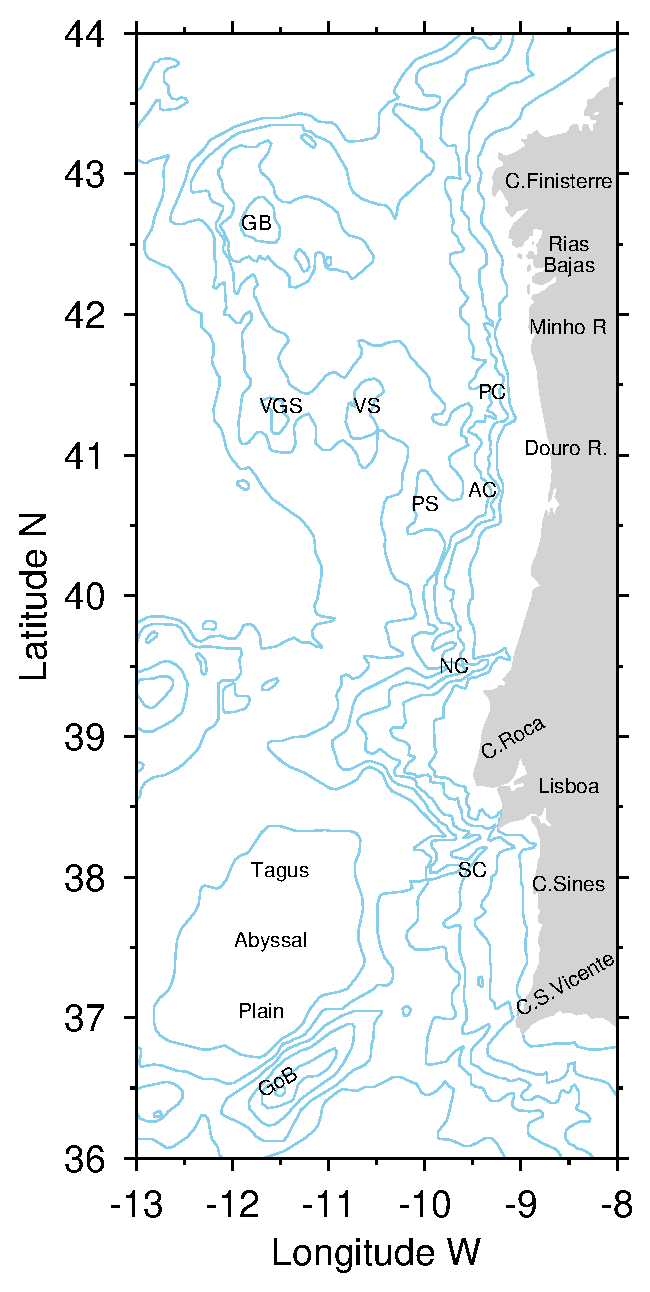
\includegraphics[scale=0.11]{bathy}
\end{minipage}
 \begin{minipage}[b]{.5\textwidth}
 \caption[Bathymetry of the Region]
 {Bathymetry and coastal morphology from GEBCO
 database showing the main features off the coast of
 Iberia from 44\deg N to 36\deg N and between 13\deg W and 8\deg W.
 Bathymetric contours at 200m and multiples of 1000m are shown.
 GB-Galician Bank, PC-Porto Canyon, AC-Aveiro Canyon, NC-Nazare
 Canyon, SC-Set\'{u}bal Canyon, VGS-Vasco de Gama Seamount,
 VS-Vigo Seamount, PS-Porto Seamount, GoB-Gorringe Bank.}
 \label{fig:largebathy}
 \end{minipage}
 \end{figure}
 The margin is cut in several places by submarine canyons which
generally define boundaries between regions with relatively
similar bathymetry conditions. North of the Nazar\'{e} canyon the
shelf is wide and very flat, with the exception of the Porto and
Aveiro canyons, as far as Cape Finisterre. Offshore of the shelf
edge, indicated by the isobath of 200m, the bottom topography is
quite complex. Between latitudes 43.5\deg and 41\deg N the
bathymetry is characterised by a deep meridional valley with a
maximum depth of 2800m separating the continental slope from the
Galicia Bank (minimum depth of 560m) to its west. The shoreline
extends almost meridionally up to about 42\deg N and then the
coast presents strong indentations (the 'Rias Bajas') as far as
Cape Finisterre. Further south at 41\deg N latitude, the Vigo,
Porto and Vasco de Gama seamounts are found. Between Nazar\'{e}
and the Lisbon region, the shelf is more irregular and is
dominated by a well pronounced zonal ridge. South of the
Set\'{u}bal canyon, the shelf is fairly flat as far as Cape Sines,
beyond which it becomes very steep until Cape S\~{a}o Vicente,
practically without a shelf break. The coastline is again
orientated very nearly in the meridional direction. At the
latitude of Cape S\~{a}o Vicente a large ridge extends offshore.
Freshwater input to the Galician shelf from the Rias (four in the
west coast and 3 in the north coast) and the Minho river is small
during summer (204\tra from mid May to mid October)
\citep{Huthnance02} but increases in winter.


\subsection{General circulation in the North Atlantic} The general
circulation in the North Atlantic (Fig.~\ref{fig:gencirc}) is
characterised by the presence of two large wind-driven gyres: the
cyclonic subpolar gyre and the anticyclonic subtropical gyre. The
subtropical gyre has its Northwest boundary defined by the Gulf
Stream (GS) which is responsible for the recirculation of the gyre
\citep{Dietrich75}. Southeast of the Grand Banks the GS separates
into two branches: the North Atlantic current, flowing to the
Northeast and feeding the subpolar gyre \citep{Clarke80,Sy88}; and
the Azores Current (AC), which crosses the North Atlantic to the
East coast between 35\deg N and 30\deg N, the exact position being
subjected to seasonal displacements \citep{Tokmakian93}.
\citet{Stramma84}, on the basis of geostrophic calculations on the
historical archive of hydrographic data, found that the eastward
flowing AC separates into three branches as it turns southward on
approaching the eastern boundary. Two branches separate west of
Madeira to make up an interior southward recirculation of the
subtropical gyre while the third passes north and around Madeira
to feed into the Canary Current.
\begin{figure}
  \centering
  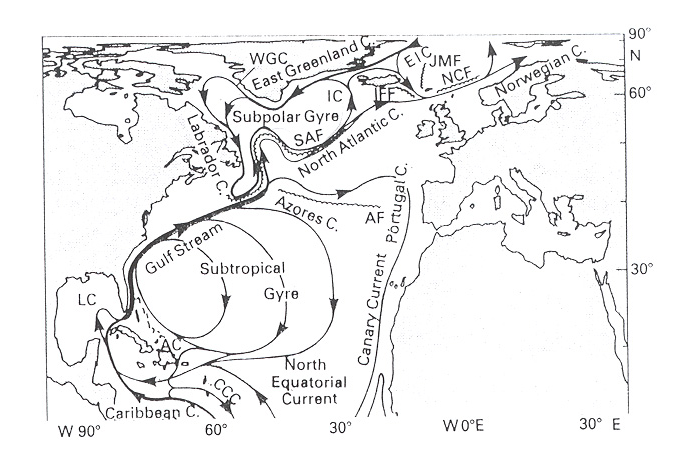
\includegraphics[height=6.5cm,width=10cm]{fig2}
  \caption{General surface circulation of the North Atlantic
  (after {\it Tomczak and Godfrey,} 1994). Abbreviations are used for
  the West Greenland Current (WGC), Irminger Current(IC), East
  Iceland Current(EIC), Loop (LC) and Antilles Currents(AC) and
  the Caribbean Countercurrent (CCC). Other Abbreviations refer to
  fronts:  Jan Mayen Front (JMF), Norwegian Current Front (NCF),
  Iceland-Faroe Front (IFF), Subartic Front (SAF) and Azores Front
  (AF).}\label{fig:gencirc}
\end{figure}

A consistent weak eastward flow of Eastern North Atlantic Central
Waters (\enaw) appears to exist off the Iberian Coast from north
of the Azores Current at depths of 200-300m corresponding to
densities lower than 27.25
\citep{Saunders82,Pollard85,Arhan94,Maze97} consistent with a
poleward shoaling of isopycnals \citep{Barton02}. Part of that
flow is later diverted off the south coast of Portugal towards the
gulf of Cadiz \citep{Maze97}. This zonal flow is associated with a
northward flow and downward entrainment with  40\% of the \enaw
entering the Mediterranean Intermediate Water (MIW) layer
\citep{Maze97} although seasonal variability can be expected in
its dynamics \citep{Saunders82,Arhan94}.

The Mediterranean outflow at the strait of Gibraltar forms MIW and
travels along the Algarve continental slope to spread out
ultimately into the Atlantic at depths between 600 and 1500m. The
MIW is evident as two maxima of temperature and salinity cores
\citep{Daniault94} and its flow is characterized by a westward
advection (mainly raised by mesoscale features as shedding eddies,
MEDDIES \citep{Kase89,Haynes90}) and turbulent diffusion of MIW
together with a well defined northward jet along the Iberian shelf
break and slope (Fig~\ref{fig:circmw}) \citep{Meincke75,Arhan94}.
The northward flow of MIW enters the Iberian slope by the Tagus
Bank between Cape S\~ao Vicente and the Gorringe Bank
\citep{Zenk90} and was named the Portugal Slope Undercurrent (PSU)
by \citet{Ambar94}. Part of the flow separates there from the
slope and flows back southwestward to the west of the Gorringe
Bank (Fig.~\ref{fig:circmw}) while the rest of the flow proceeds
northward in the form of a Slope Undercurrent \citep{Daniault94}
with a characteristic transport of 7.6 $10^6$ \tra \citep{Maze97}.
The MIW slope current divides later into two branches between
41\deg N and 42\deg N, a western branch flowing to the west of the
Galician bank and a coastal branch following the shelf break in
response to the  steering effect of bottom topography.  A further
effect of the bottom topography-flow interaction of the PSU is the
existence of a bottom boundary Ekman layer enhancing downslope
Ekman transport.

In the same region the Central Waters flow strongly resembles that
of the MIW, suggesting a vertical coupling of both water masses.
\begin{figure}
  \centering
  \includegraphics[height=11cm,width=9cm]{fig3}
  \caption{Schematic circulation of MW in May 1989 in the Iberian
  coast. Black dots represent CTD stations. Reported numbers are volume
  transports in $10^6$ \tra [from {\it Maz\'e et al.,} 1997].}
  \label{fig:circmw}
\end{figure}
\subsection{Weather Regime} Upwelling occurs all along the East
coast of the central North Atlantic from the northern tip of the
Iberian peninsula to south of Dakar at almost 10\deg N, as a
result of the characteristics of the wind. During the summer
months, when the Azores high-pressure cell is located in the
central Atlantic and the Greenland low has diminished in
intensity, the resulting pressure gradient forces the air to flow
southward along the coast of Iberia inducing upwelling and
associated southward circulation. In contrast, in winter the
Azores high-pressure cell is located further south, off the
northwestern African coast, and a deep low is located off the
southeastern coast of Greenland. The pressure gradient between the
two pressure systems results in an onshore wind with a component
of wind stress northward off Iberia.

\citet{Blanton87} showed that there are large interannual
variations in upwelling in response to the large-scale meteorology
variations in the North Atlantic. The continuously varying
strength and position of the Azores High and the Greenland Low
lead to variations in the strength and direction of upwelling
favourable winds at these latitudes.

\subsection{Coastal circulation} The general structure of the
Portugal Current System off the west Iberian coast is formed by
the following basic components \citep{Fiuza96b}:
\begin{enumerate}
  \item  a large scale southward surface flow in the open ocean,
  seaward of the continental margin related to the N. Atlantic
  subtropical gyre, the Portugal Current,
  \item an equatorward surface flow over the slope, in the
  vicinity of the shelfbreak during the upwelling season
  (June-July until late September), the Portugal Coastal Current,
  \item a poleward surface flow along the upper slope from
mid-autumn until late spring, the Portugal Coastal Countercurrent,
  \item the semi-permanent poleward Portugal Slope Undercurrent.
\end{enumerate}
Bearing in mind that none of the above currents are restricted to
the Portuguese margin they would be better named the Iberian
currents.
\subsubsection{Winter regime}
\begin{figure}
  \centering
  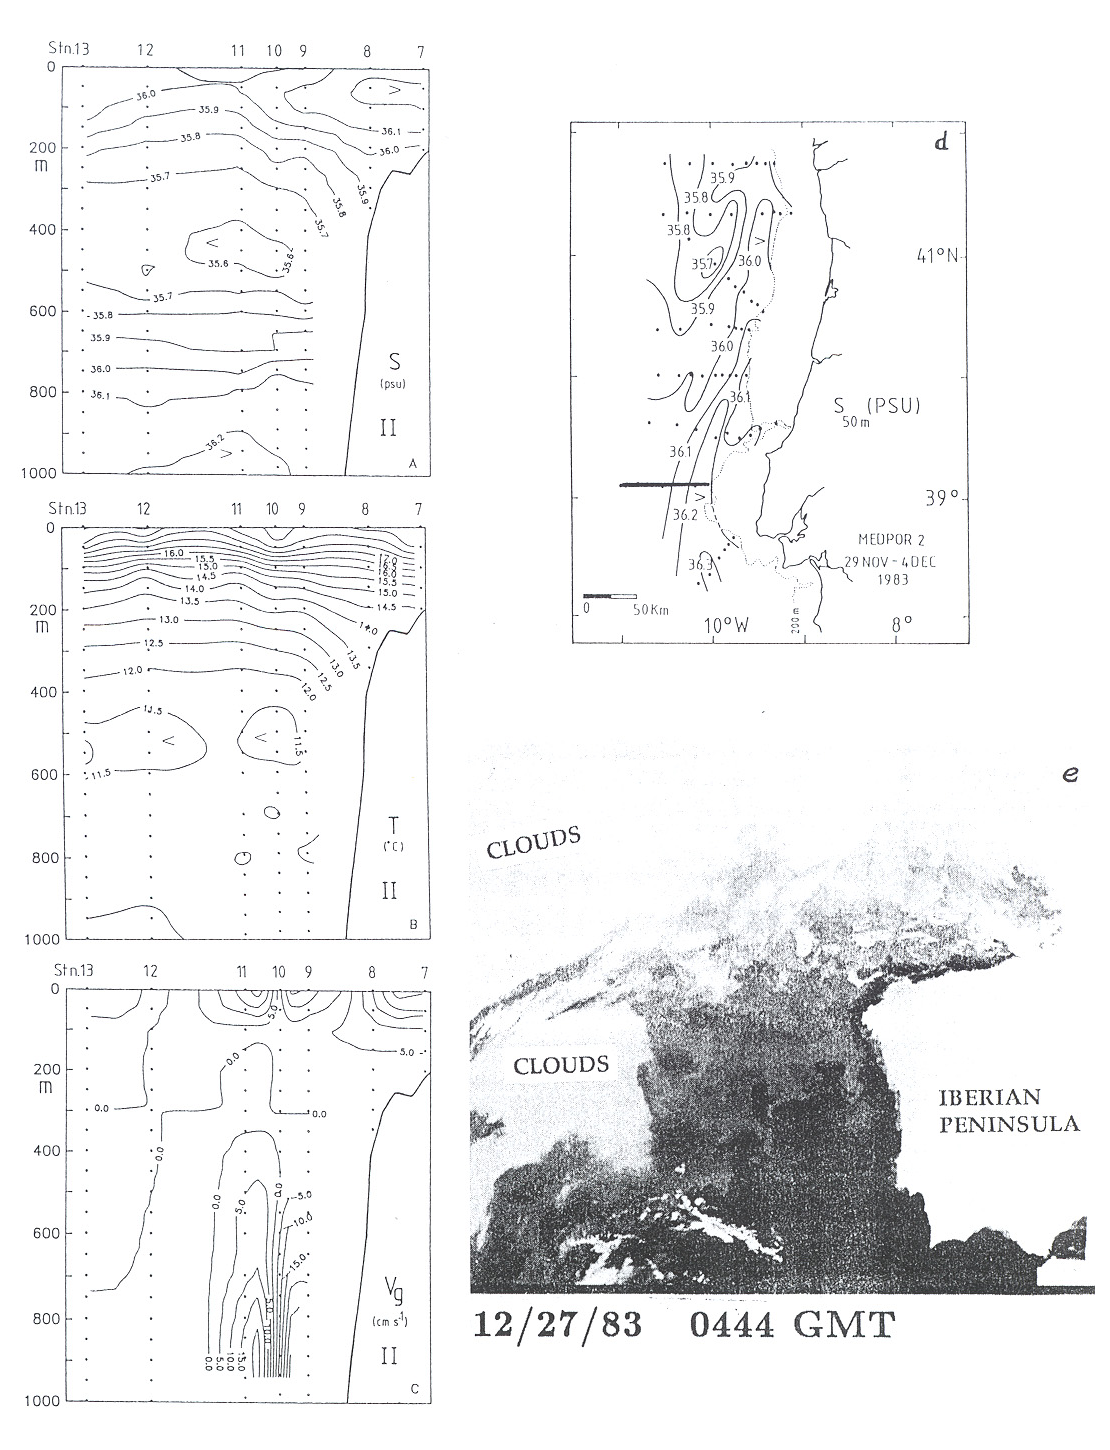
\includegraphics[width=16cm]{fig4new}
  \caption{Different signatures of the PCC from winter 1983.
  Vertical distribution of (a) salinity, (b) temperature, and (c)
  meridional component of geostrophic velocity relative to 300
  dbar along section II (thick line in d). Salinity distribution
  at 50m (d) showing the PCC (saline intrusion) along the slope.
  Thermal infrared picture (e) from the NOAA 7 satellite where
  darker tones corresponds to warmer temperatures [from {\it Frouin et
  al.,} 1990].}\label{fig:poleward}
\end{figure}
The meteorological conditions offshore from the Iberian Peninsula,
governed by the meridional displacements of the Azores High as
mentioned before, show distinct winter and summer regimes.  In
winter, the weakening and southward migration of the anticyclone
places the north of the region under the influence of
southwesterly winds. The upper layer circulation in this season is
characterised by the presence of a narrow northward slope current
which settles in November and disappears around May
\citep{Frouin90,Haynes90,Pingree92}. This structure
(Fig.~\ref{fig:poleward}) appears as a warm and saline intrusion
(temperature 1-3\deg C and salinity 0.2-0.3psu higher than
surrounding values), trapped within about 50km of the shelf break,
about 200-600m deep. It flows along the slope with characteristic
velocities of 0.2-0.3\vel, and extends more than 1500km and with
transport increasing in the flow direction
\citep{Frouin90,Haynes90}. Drifter experiments
(Fig.~\ref{fig:morenadrifters}) have revealed a meandering surface
flow with eddies of different scales superimposed on the poleward
mean flow \citep{Haynes91,Sena96}. This Portugal Coastal
Countercurrent (PCC),\citep{Fiuza97}, flows along a semi-permanent
front separating the fresher shelf waters influenced by the winter
river runoff from rivers of northern Portugal particularly from
the Douro, from the open ocean \citep{Hamann96}. That convoluted
front was observed to contribute to the shelf-ocean exchange via
mesoscale cyclonic eddies (10-20km in diameter) which are shed
into the open ocean from the Countercurrent
\citep{Fiuza96b,Perez01}. Other active exchange processes are
mixing and entrainment into the poleward Countercurrent of shelf
waters which are advected alongshore for hundred of kilometres
before dispersing into the open ocean with an estimated residence
time on the shelf of 1-2 months\citep{Fiuza96b}. Those fronts are
common features of the shelf breaks as a result of buoyancy inputs
and their ``anchorage" at the shelf break is a response to
potential-vorticity conservation and geostrophy \citep{Condie93}.
As mentioned above, the slope current extends downwards including
the MIW to a depth of 1500m and more, as reported by
\citet{Huthnance02} at various moorings along the Iberian Atlantic
coast outside the shelf break.
\begin{figure}
  \centering
  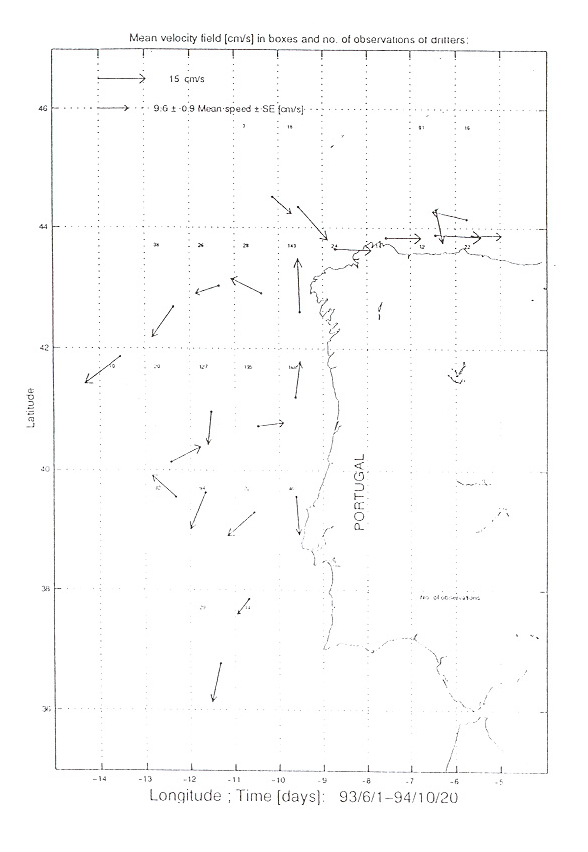
\includegraphics[height=9cm]{fig5anew}
    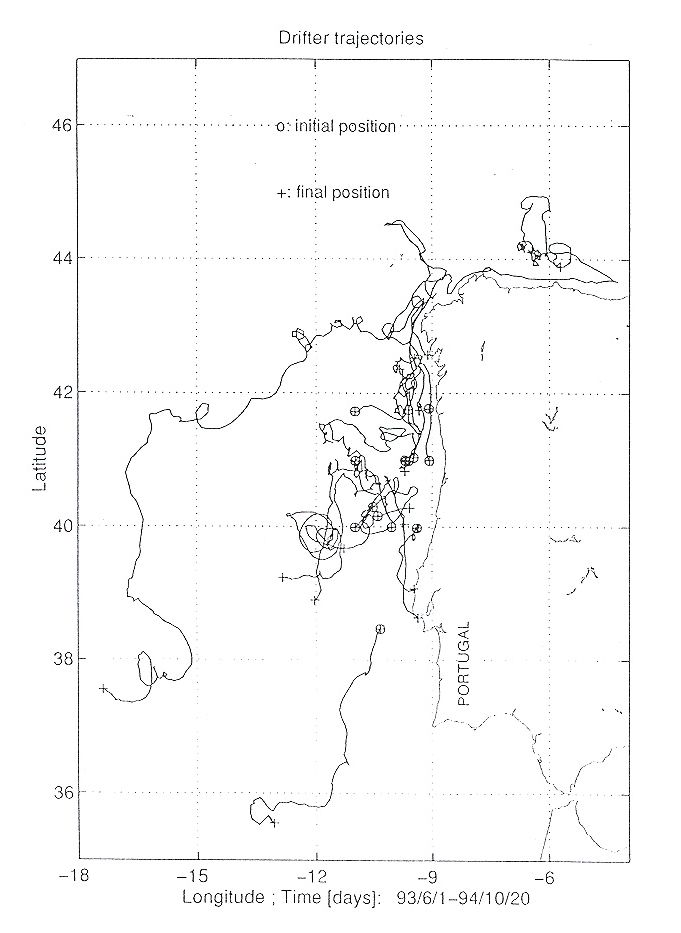
\includegraphics[height=9cm]{fig5bnew}
  \caption{Mixed layer drifter tracks (right) and derived surface
  velocities (left) for 16 drifters used in the MORENA project
  during June 1993-October 1994. 11 drifters were released during
  November 1993 and their trajectories correspond to the period
  November 1993-May 1994 [{\it Sena,} 1996].}\label{fig:morenadrifters}
\end{figure}

\citet{Pollard85} described a meridional density gradient in the
upper 200-300m associated with the poleward cooling of the sea
surface which can force a poleward current that becomes
intensified over the slope and which increases along the flow
\citep{Huthnance84}. The winter wind circulation could also
generate a poleward slope current and the two mechanism were found
to actively drive the PCC \citep{Frouin90}.

Large and persistent anticyclonic warm slope-water eddies
(SWODDIES) have been associated with the PSU in winter if the warm
flow is strong \citep{Pingree94} in relation with the instability
of the slope current in the Bay of Biscay
(Fig.~\ref{fig:swoddies}) although no consistent seasonal
variability has been established. They have characteristic radii
of 50-60km, a signature discernible in the upper 1500m, and a
lifetime of about a year. \citet{Pingree93} also identified eddies
shed from the slope at Cape St. Vincent, Setubal canyon and Lisbon
canyon in respond to the complex topography
(Fig.~\ref{fig:swoddies}b and c) and the persistence of a
topographic eddy is suspected over the Galician Bank
\citep{Hill98}.

There has been reported evidence of poleward flow south of 35\deg
N \citep[i.e. off NW Africa][]{Barton90,Mittelstaed91} which shows
seasonal persistence, although its connection with the PCC is not
yet established.
\begin{figure}
  \centering
  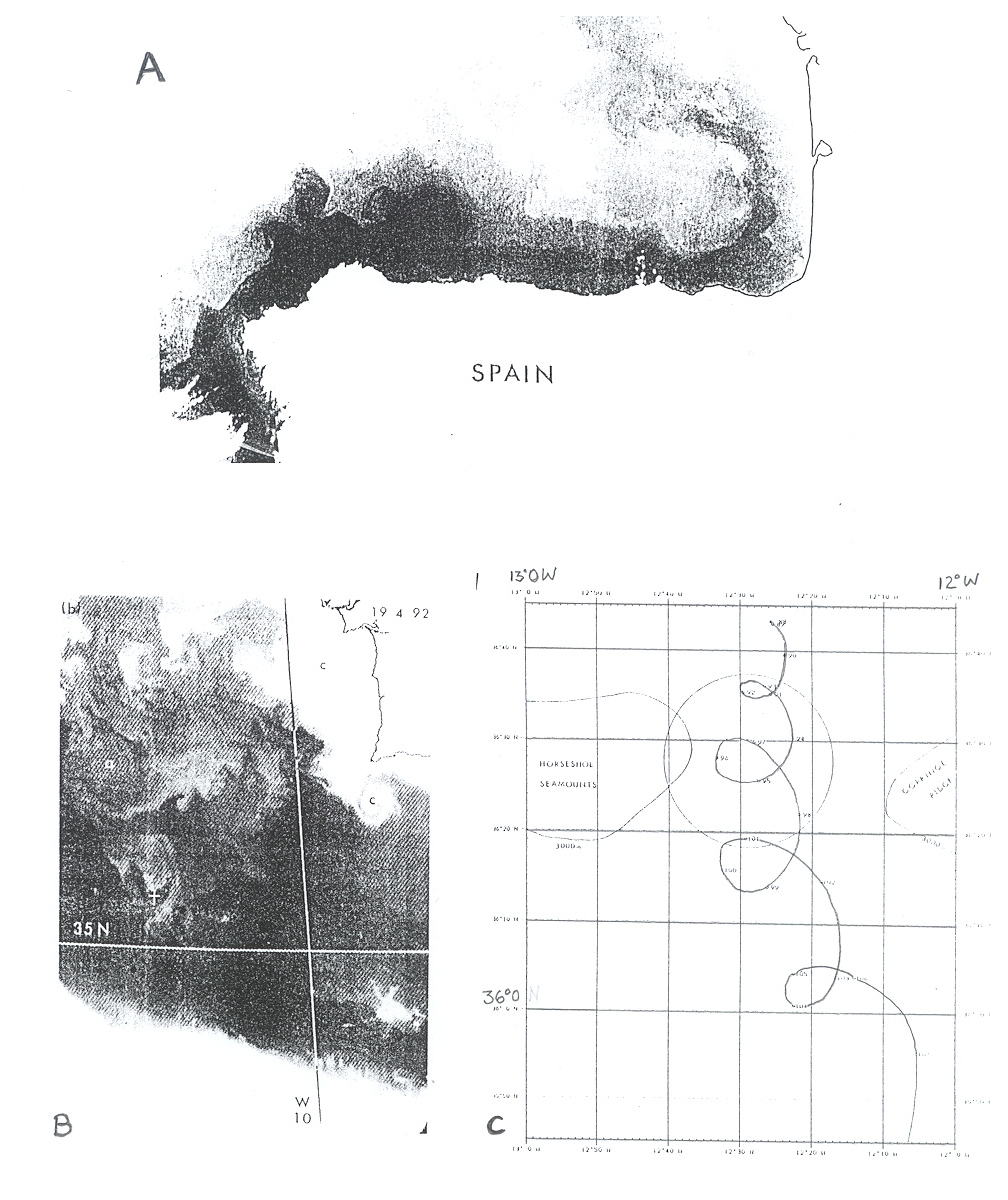
\includegraphics[height=14cm]{fig6new}
  \caption{Eddy signatures along the Iberian coast. (a)  Infrared
  image (NOAA 10, 28 Dec. 1989) showing warm surface water flowing
  along the west and northern Spanish slopes and swoddy formation.
  (b) Infrared image (NOAA 12, May 5, 1992) showing the
  development of a cyclonic eddy off Cape St. Vincent (labelled
  c). (c) Track of buoy 3906 (drogued at 800m) with daily
  positions marked, showing typical 4-day period and southward
  translation (~5km/d). A circle of 35km is shown to indicate the
  scale of the eddy core. ((a) from {\it Pingree and LeCann} 1990, (b,c)
  from {\it Pingree and LeCann} 1993).}\label{fig:swoddies}
\end{figure}
\subsubsection{Summer regime} In the North Atlantic the summer
Trade winds have a strong alongshore component which drives
upwelling off Iberia from May to October as described in the early
works of \citet{Wooster76} and \citet{Fiuza82b}. A more detailed
study of the wind regime in the coasts of the Iberian Peninsula
was made by \citet{Bakun91} who calculated wind stress and curl of
wind stress on a 1x1\deg  grid from historical merchant ship
records. Their results showed that the near shore region from
Iberia to 15\deg N is characterised generally by cyclonic
wind-stress curl (Positive) during the upwelling season, which
causes in turn a divergence and consequent Ekman pumping enhancing
the coastal upwelling. However, local wind patterns near the coast
may be significantly affected by orographic influences due to the
presence of capes and Rias locally enhancing upwelling
\citep{Mcclain86}.

The upwelling favourable winds during the summer have a marked
oscillatory pattern from March till October as revealed by
harmonic analysis of 9 years of daily averaged upwelling indices
deduced from geostrophic winds estimated for a cell centred at
43\deg N 11\deg W, 150km off Cape Finisterre \citep{Nogueira97}.
The wind displays a quasi-periodic component of T=15$\pm$5 days
during the upwelling season. This time structuring is imposed on
the shelf ecosystem and is in part responsible for the high
productivity of the area. Further south, in the Portuguese
Atlantic coast, periods were found to be of 6-7 days
\citep{Sousa86}. \citet{Nogueira97} also concluded that the
downwelling season has a less regular pattern, with the dominant
mode of variation being T$\sim 30\pm$20 days.
\begin{figure}
  \centering
  \includegraphics[height=6cm,angle=-90]{fig7anew}
  \includegraphics[height=6cm,angle=-90]{fig7bnew}
  \includegraphics[height=12cm]{fig7c}
    \caption{(a) Location of stations sampled in August September
  1981. (b) Section showing the meridional component of
  geostrophic velocity (computed relative to 300 dbar and
  expressed in \velc ); negative values represent southward flow
  [{\it Fiuza }1983]. (c)Temperature distribution at 50dbar in September
  1994 showing the anchorage of the upwelling front to the shelf
  break [{\it Fiuza }1996].}
  \label{fig:summerupw}
\end{figure}

 Continental shelf and slope waters off the western and southern
Iberian Peninsula are dominated during the summer months by strong
coastal upwelling. The associated baroclinic equatorward jet
(Fig.~\ref{fig:summerupw}), the Portugal Coastal Current (PCoC)
\citep{Ambar94}, attains velocities of 15-20\velc
\citep{Fiuza84,Mcclain86}. A strong temperature front, separating
the cold recently upwelled water from the offshore oceanic water
(Fig.~\ref{fig:summerupw}), develops in close relation to the
bathymetry of the continental shelf and slope and to the coastal
morphology \citep{Fiuza83}. The time response of the system to
local wind forcing was estimated by \citet{Sousa86} to be less
than 24hrs in the Portuguese coast, as expected from such a
dynamic system, although \citet{Mcclain86} give values of 3 days
for the Galician coast. The time evolution of the system includes
further distortion of the front and development of meanders,
eddies and filaments following a seasonal pattern
\citep{Haynes93}.

During the upwelling period, the wind forcing is opposite to the
poleward density gradient but the PCoC equatorward geostrophic jet
is enough to counter the poleward slope current at and near the
surface so that southward flow is established. However, below
100-200m the flow is still poleward \citep{Haynes90,Huthnance02}.
Spectral analysis of long-term moored current-meters have shown
the presence of signals in the period range of 40-70hrs, which
match the characteristics of the second mode of continental shelf
waves compatible with the local stratification and bottom
topography \citep{Fiuza96}. This waves could play a significant
role in accommodating the eastward flow of ENAW
\citep{Huthnance95} and in driving part of the poleward
undercurrent as suggested in the Californian upwelling system
\citep[e.g.][]{Wang97}. Their relevance in the Iberian system is
yet to be established.

\subsubsection{Patterns of mesoscale variability}
Early in the eighties, \citet{Fiuza83} suggested the strong
3-dimensionality of the Iberian Upwelling system identifying an
upwelling front strongly deformed by meanders, mesoscale eddies
and filaments (Fig.~\ref{fig:litomexfil}), cold tongues of
recently upwelled waters extending offshore some hundreds of km.
Capes such as Cape St. Vincent \citep{Sousa86,Relvas99}, or Cape
Finisterre \citep{Blanton84} are also involved in the promotion of
localized or intensified coastal upwelling introducing an
important component of spatial variability into the system.
\begin{figure}
  \centering
  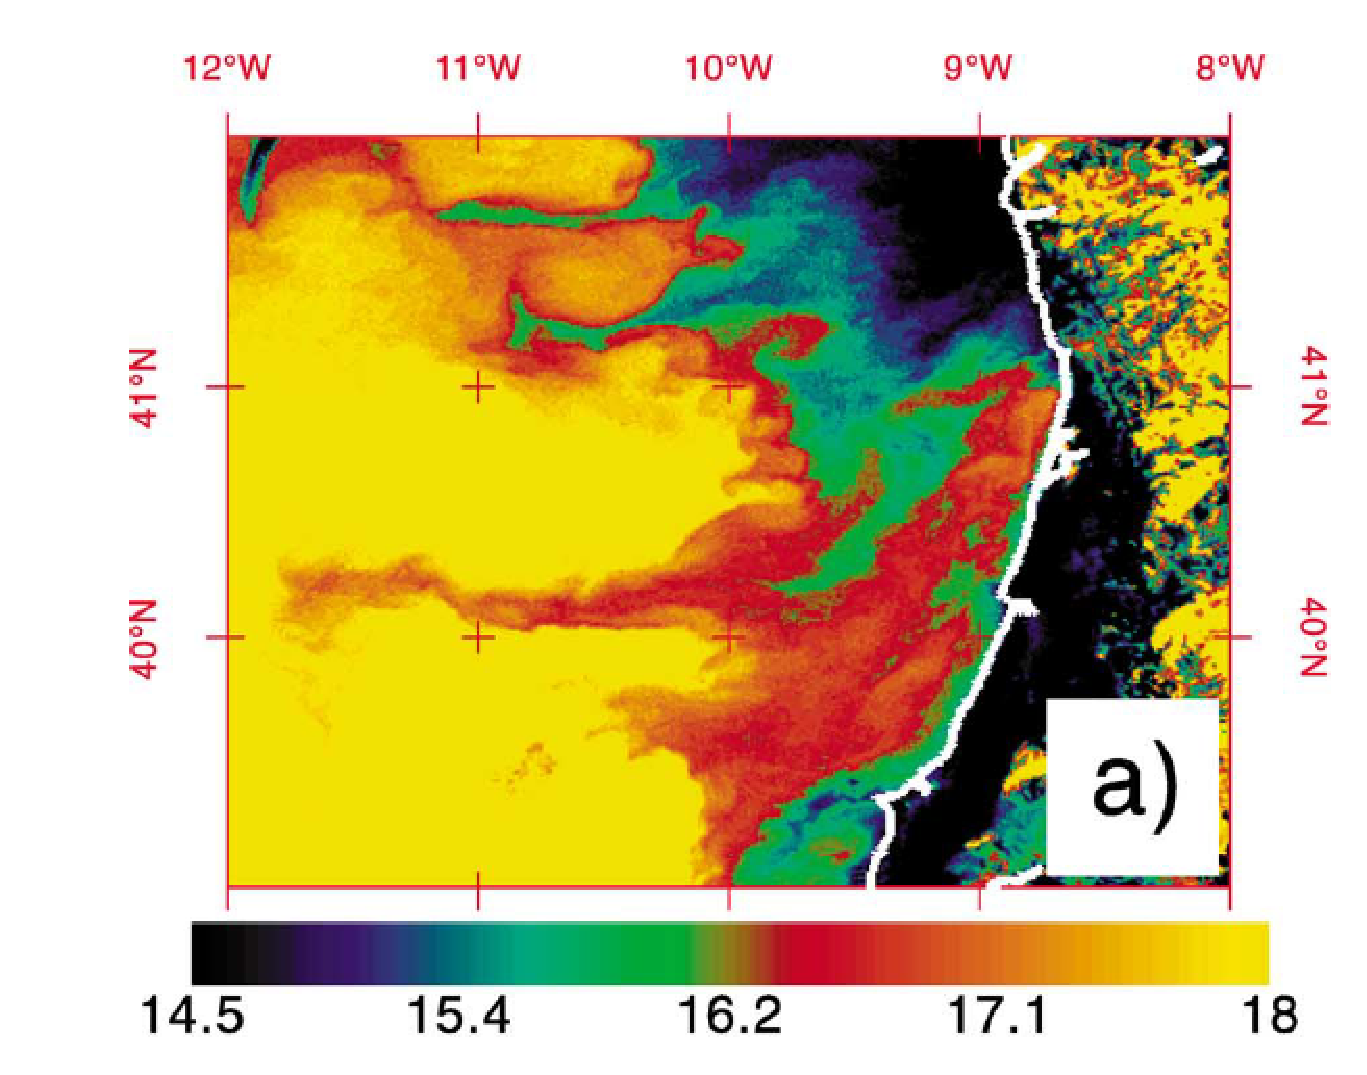
\includegraphics[height=10cm]{filaments}
  \caption{AVHRR Channel 4 brightness temperatures of the Western
  Iberian coast. (a) NOAA-14 in 24/08/98 at 03:58 UTM.
 The HRPT data were received at the Dundee
Satellite Receiving Station and processed at IPIMAR [{\it Peliz et
al., }2002] }
  \label{fig:litomexfil}
\end{figure}

The large mesoscale features of the region, in particular the
filaments, follow a strong seasonal fluctuation similar to the
California Upwelling System, in strong relation to the seasonal
wind pattern. At the beginning of the upwelling season, May-June,
a narrow band of colder water of quite uniform width develops
along the coast, often consisting of many narrow ``fingers'' of
cool water extending 20-30km offshore \citep{Haynes93}. Those
features have been successfully modelled in a 1\onehalf \, layer
model by \citet{Roed96} for the Iberian region including realistic
topography and coastline geometry. Linear stability analysis has
also suggested that front waves of wavelengths about 20km appear
first \citep{Barth94} in response to frontal instability
\citep[e.g.][]{Washburn88,McCreary91}] which feeds from potential
energy stored in the lateral density gradient.

\begin{figure}
  \centering
  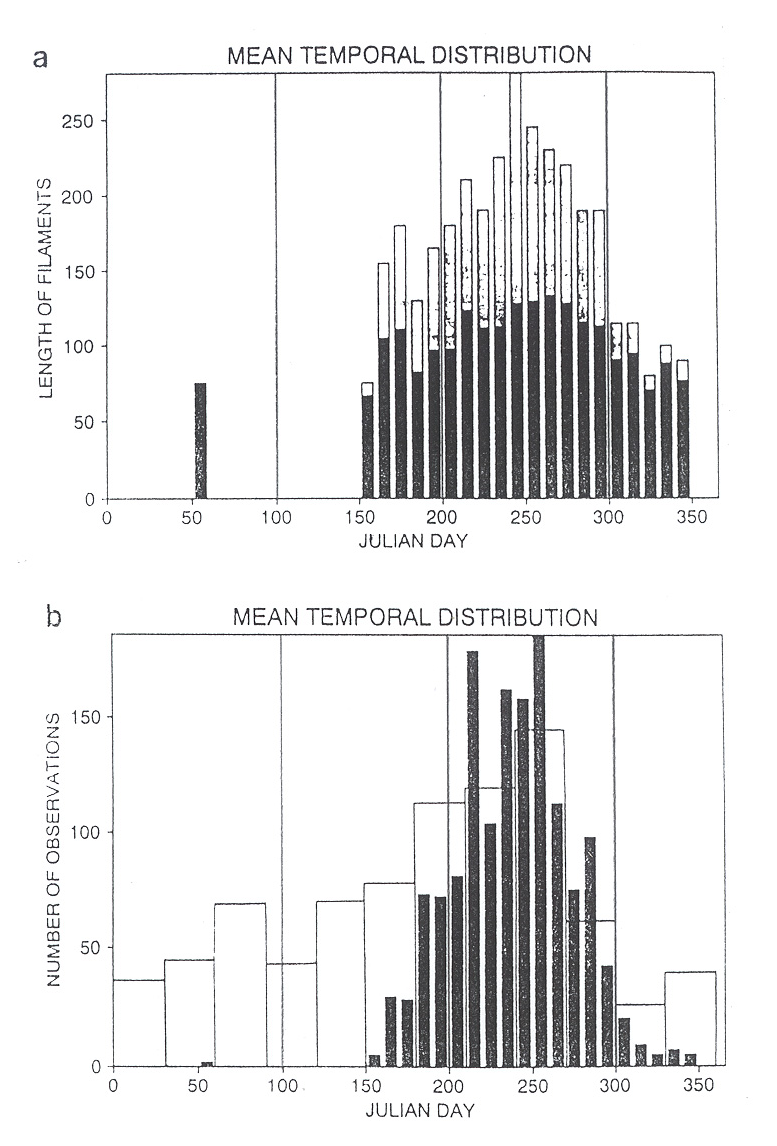
\includegraphics[height=16cm]{fig9new}
  \caption{(a) Temporal evolution of the mean length (solid bars)
  and greatest observed lengths (grey bars) of filaments from the
  brightness temperature scene archive (1982-1990). (b) Temporal
  evolution of the number of observed filaments per 10 day
  interval (solid bars). Open bars indicate the number of images
  available for 30-day periods [{\it Haynes et al., }1993].}
  \label{fig:filstats}
\end{figure}
The narrow band might temporarily disappear after relaxation or
poleward wind events and is not until July or August that the
fingers merge in preferred locations to form filament structures.
Statistical analysis from \citet{Haynes93} spanning over 9 years
(1982-1990) showed filaments reached a mean length of 80km (30km
seaward of the upwelling coastal band) in July and then continued
growing until reaching a maximum mean length of 130km in late
September (Fig.~\ref{fig:filstats}). Similar growth rates were
found for the largest filaments which can reach over 250km in late
September. Filaments seem to weaken towards the end of October and
to disappear on a time scale of the order of a week once upwelling
stops \citep{Haynes93}. Similar seasonal increase in the strength
of mesoscale meanders, filaments  and eddies was observed for the
Californian System during one year GEOSAT altimeter data by
\citet{Flament89}. The expected lifetime of the filaments ranges
from 1 to 3 months \citep{Haynes93,Sousa95}.

\citet{Strub91} suggested three possible mechanisms for filament
formation, namely ``squirts'', meandering jet and pre-existent
eddy field. Only the  first two were identified as possible
generating processes in the Iberian System \citep{Haynes93}.
``Squirts'' respond to nearshore convergences while the meandering
jet has been identified as a consequence of baroclinic instability
and both are affected by the coastline and bathymetry as suggested
by \citet{Sousa92} and \citet{Haynes93} for the Iberian filaments.
The pre-existent eddy field implies that eddy pairs interact to
drag cold water seaward but the deterministic nature of the
filaments means that a truly random interaction of oceanic eddies
with the coastal transition zone is not possible.
%\begin{figure}
%  \centering
%  \includegraphics[height=18cm,width=14cm]{blank}
%  \caption{Meridional temperature profiles along part of the
%  Iberian coast ( 42.5\deg N-40\deg N, 10\deg W) during the upwelling season
%  of 1982 together with the bathymetry section of the same line at
%  50km from the coast ({\it Mendes de Sousa} 1995).}
%  \label{fig:filridges}
%\end{figure}

\citet{Haynes93} identified 5 major filaments in the Iberian coast
which recur every year in the same position. They are associated
with topographic features of the region, mainly capes such as Cape
Finisterre and Cape Ortegal in the Galician coast of Iberia and
Cape Roca, Cape Sines and Cape S\~ao Vicente in the Portuguese
coast. Their results were later confirmed by \citet{Sousa95} in a
similar analysis of 11 years of AVHRR data (1979-1989) in which
filaments were consistently associated with submarine ridges.
Laboratory experiments in a rotating tank \citep{Narimousa89} have
successfully reproduced a meandering upwelling yet and filaments
in the presence of ridges owing to the topographic effect and
potential vorticity conservation. Modelling work done by
\citet{Roed96} also reproduced the observed distribution of the
Iberian filaments and their time persistence. Energy consideration
within the model identified frontal instability as the baroclinic
instability responsible for the generation and growth of eddies
and filaments, while potential vorticity considerations suggested
that coastline and topography irregularities provide sufficient
background perturbation for the frontal instability mechanism.
\begin{figure}
  \centering
  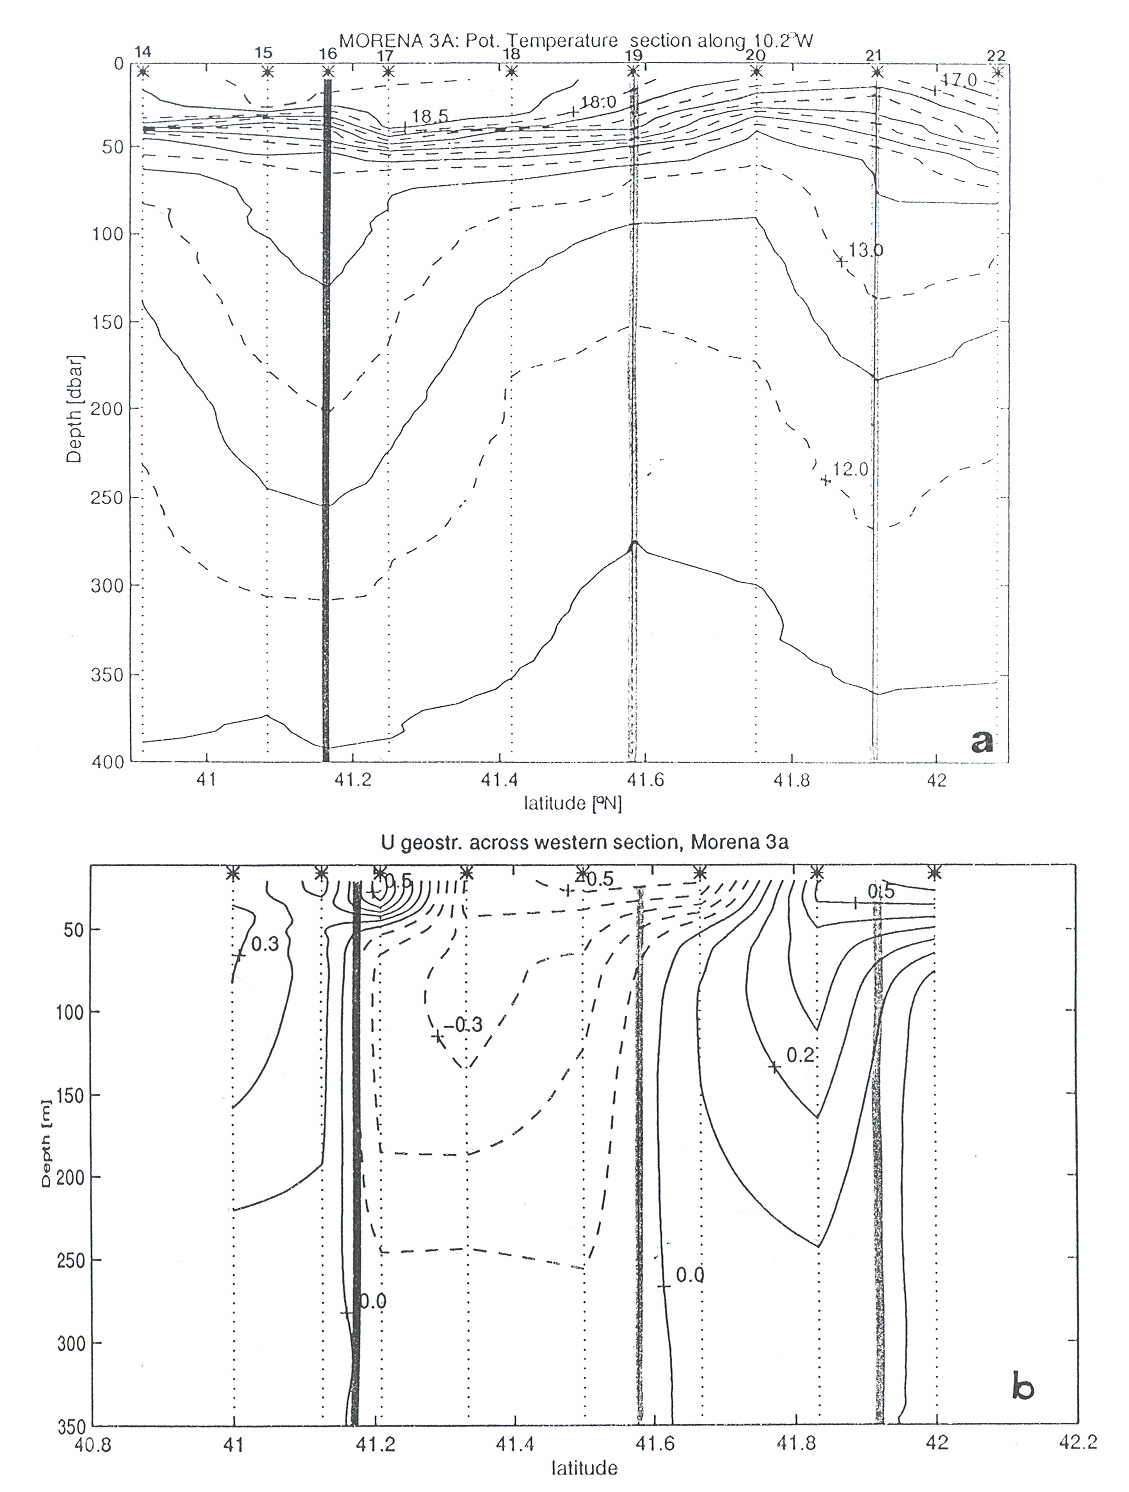
\includegraphics[height=16cm]{filamentsectionnew}
  \caption{(a) Meridional temperature section along 10.2 W carried
  out in the 6-7 August 1994 and (b) geostrophic velocity section
  along the same line calculated relative to 350dbar. Positive
  values indicate offshore velocities [{\it Fi\'uza }1996].}
  \label{fig:morenafil}
\end{figure}

Few in situ surveys have been carried out to determine the 3-d
structure of filaments,  the recent MORENA project being one of
the best examples \citep{Fiuza96b}. Hydrography and ADCP surveys
showed filaments extended 100-200km offshore. They were 30-50km
wide and penetrated to 250m deep  near their shelf-edge ``root'',
but diminished offshore  to 20-30km in width and 50m in depth. The
classical view of strong offshore baroclinic flow was supported by
the geostrophic velocities calculated from the hydrographic data
which displayed a surface core velocity of 0.5\vel decreasing to
about 0.05\vel\, at depths of 150-200m (Fig.~\ref{fig:morenafil}).
Some irreversible mixing of filament and ocean waters is expected
and filaments would play an important role in the exchange between
the shelf and ocean \citep{Huthnance95}.

Dynamic features of the upwelling system off the Western Iberian
coast, like the 'event' scale variability, the existence of a
frontal alongshore jet, and the omnipresent poleward slope
undercurrent have parallels in all the major upwelling regions
\citep{Barton98}. A summary of the main characteristic of the
Iberian upwelling can be seen in Table~\ref{tb:lit_summ}.
{\linespread{1}
\begin{table}[h]
  \centering
\begin{small}  \begin{tabularx}{400pt}{XXXXX}
  \textbf{Principal climatic influence} &\textbf{Principal Oceanic influence}  &\textbf{Topography}&\textbf{Freshwater
  influence}&\textbf{Winds}\\
  Azores High &Portugal Current&Narrow shelf&Small, Spanish Rias in the north&NE trades (summer) \\
  \hline
  \textbf{Tides}&\textbf{Poleward flow}&\textbf{Equatorward flow}&\textbf{Upwelling}&\textbf{Filaments}\\
  Internal tide generations, solitons&Along shelf edge, turn 90\deg to flow along North Spanish slope& Portugal Coastal Current&
  37\deg-43\deg N &130km mean, 270km maximum, 5 main sites\\
  \hline
  \textbf{Fronts}&\textbf{Eddies}&\textbf{Quasi-permanent eddies}&\textbf{Coastal Trapped Waves}&\textbf{Short-term variability}\\
  Upwelling fronts&Generated off Cape St Vincent&Over offshore banks?&Not known&Not known\\
  \textbf{Seasonal variability}&\textbf{Interannual variability}&\textbf{Special
  features}&&\\
  Upwelling in summer, Poleward flow in winter&Not reported&Divided from NW Africa eastern boundary by Strait of Gibraltar&&\\
  \hline \hline
  \end{tabularx}
   \end{small}
  \caption{Summary of Phenomena and Processes in the
  Iberian Eastern boundary.}\label{tb:lit_summ}
\end{table}
}
\subsection{Water-Masses in the Iberian coast }
The NW Iberian upwelling region is the least productive  of the
oceanic eastern boundaries \citep{Castro00}. Pacific and Indian
oceans present considerably higher nutrients and lower oxygen
levels than the Atlantic ocean \citep{Levitus93}. The Galician
coast is situated in the region of the ventilated thermocline
where \enaw forms \citep{Rios92}, and consequently, \enaw upwelled
along the Galician coast exhibits low nutrient enrichment by
oceanic ageing compared to \enaw that upwells off the African
coast \citep{Castro00}.

Different water masses can be identified off the Iberian Atlantic
coast where the water column can be divided into upper (first
100-200m), intermediate (to a depth of 1300) and deep (from 1300m
to the bottom) layers.
\begin{figure}
  \centering
  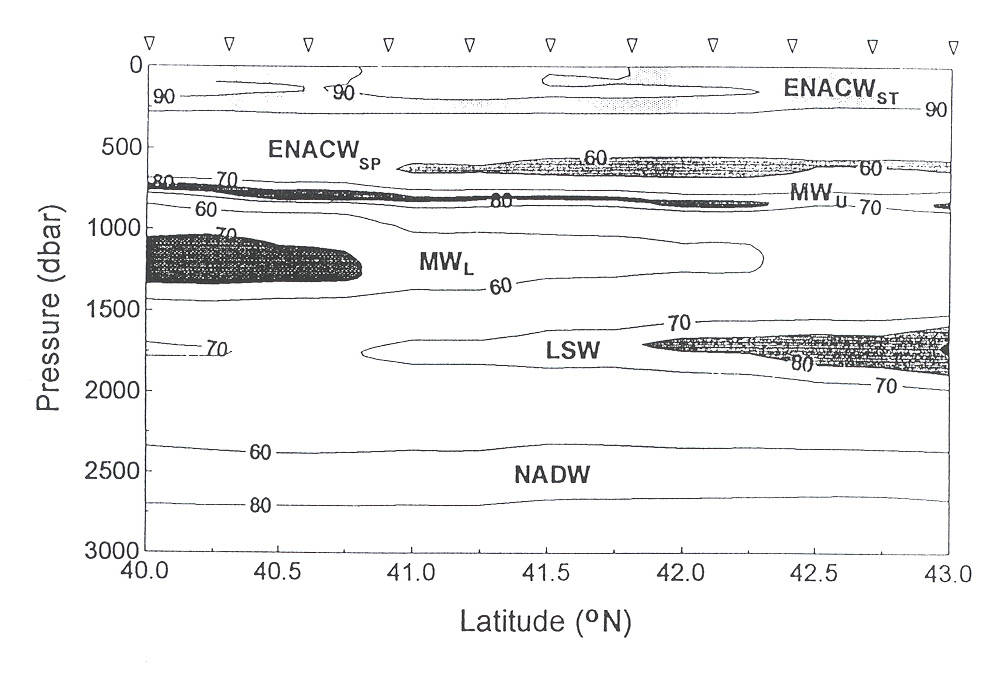
\includegraphics[width=13cm]{watermassnew}
  \caption{Percentages of the different water masses as indicated
  by their abbreviated designations (st and sp meaning subtropical
  and subpolar respectively), calculated using $\theta$/S mixing
  triangles along a meridional section at 10\deg W. The positions of
  the CTD stations collected during May 1993 are indicated by
  small triangles along the top of the figure [{\it Fi\'uza et
  al.,} 1997].}
  \label{fig:ctdmixing}
\end{figure}

The upper layer during winter months corresponds to a mixed layer
produced by wind stress mixing, of surface fresh water from
precipitation and river runoff, while during summer months it
displays a seasonal thermocline. Below the thermocline, \enaw can
be identified. Recently the \enaw has been subdivided by various
authors depending on its provenance. North of 46\deg N, the
formation of the subpolar mode of \enawp takes place during the
winter ventilation in the Atlantic subpolar gyre and it is
characterised by temperatures and salinity between 4\deg C, 34.96
psu and 12\deg C, 35.66psu \citep{Rios92}. The warm and salty
subtropical mode, \enawt, forms near the Azores front at about
34\deg N as a result of evaporation and deep winter convection
\citep{Fiuza84}. It is carried eastward by the Azores current
until the northern vicinity of Madeira where it splits into an
anticyclonic branch constituting the southward Canary Current and
a cyclonic branch flowing poleward along the western Iberian
slope, the PCC \citep{Fiuza97}. The characteristics of the \enawt
are defined as 12.2-18.5\deg C and 35.66-36.75psu
\citep{Fiuza82a,Rios92}, coinciding in part with the definition of
North Atlantic Central Water given by \citet{Helland-Hunsen26}.
Both characteristic lines can be seen in Fig.~\ref{fig:litts}.

The upwelled water is generally the subtropical mode of \enawt ,
Fig.~\ref{fig:litts}, but \enawp can also be found in the north
($>$ 40\deg N), underlying the subtropical mode at depths between
250 and 550m. The southward jet-like surface flow then transports
both \enaw branches towards the south along the upper slope/outer
shelf zone. The poleward extent of the subtropical ENAW is
strongly related with the PCC but its northern most limit
constitutes the subsurface front (Galicia Front) in the region of
Cape Finisterre (43\deg 30'N) between \enawt and \enawp
\citep{Fraga82,Fiuza84}. The Galicia front has recently been
identified by a strong pigment signal in CZCS images suggesting
localized phytoplankton blooms \citep{Peliz96}.

The upper layer along the Portuguese coast exhibits significant
variability particularly in its salinity signature
(Fig.~\ref{fig:litts}), ranging from 35.0psu to 36.2psu due to a
combination of surface warming, upwelling of central waters (both
\enawt and \enawp ) and mixing with river runoff \citep[][in
preparation]{Barton02}.
\begin{figure}
  \centering
  \subfigure[]{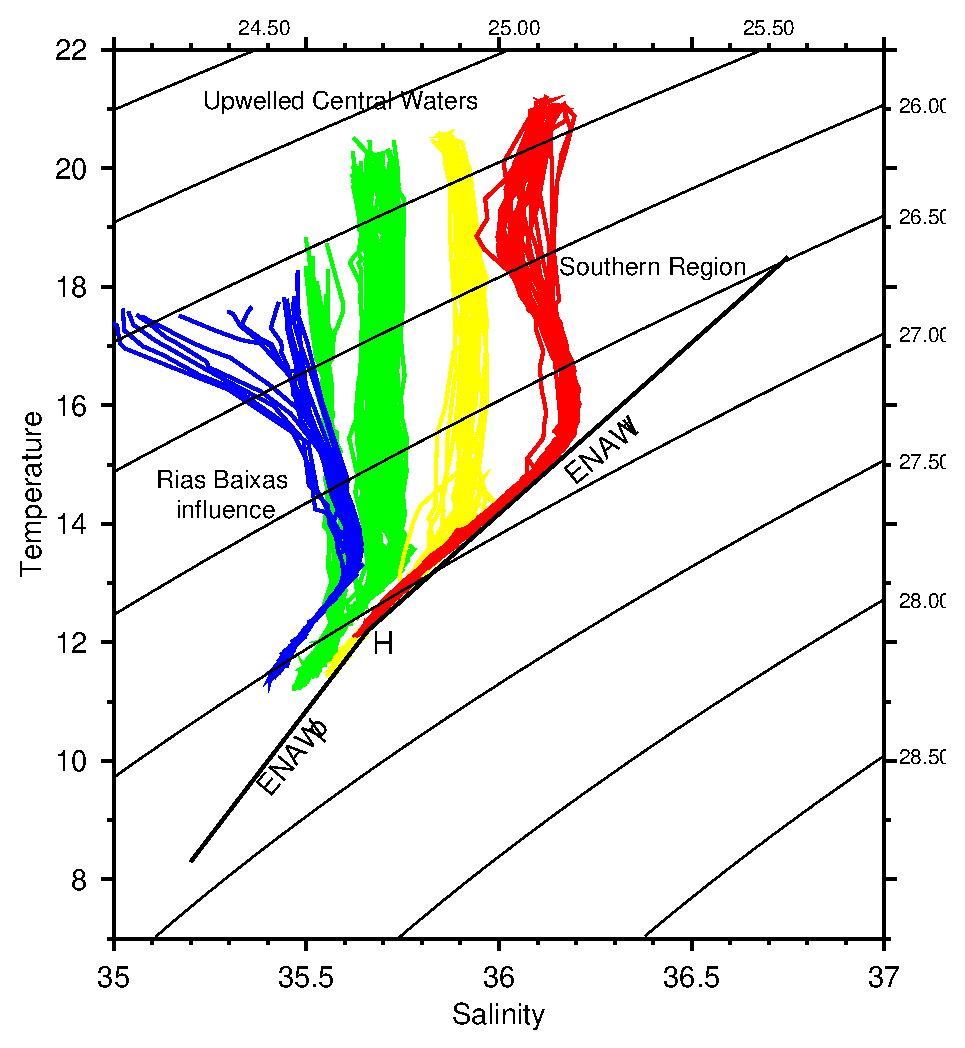
\includegraphics[height=8cm]{ts_diag1}}
  \subfigure[]{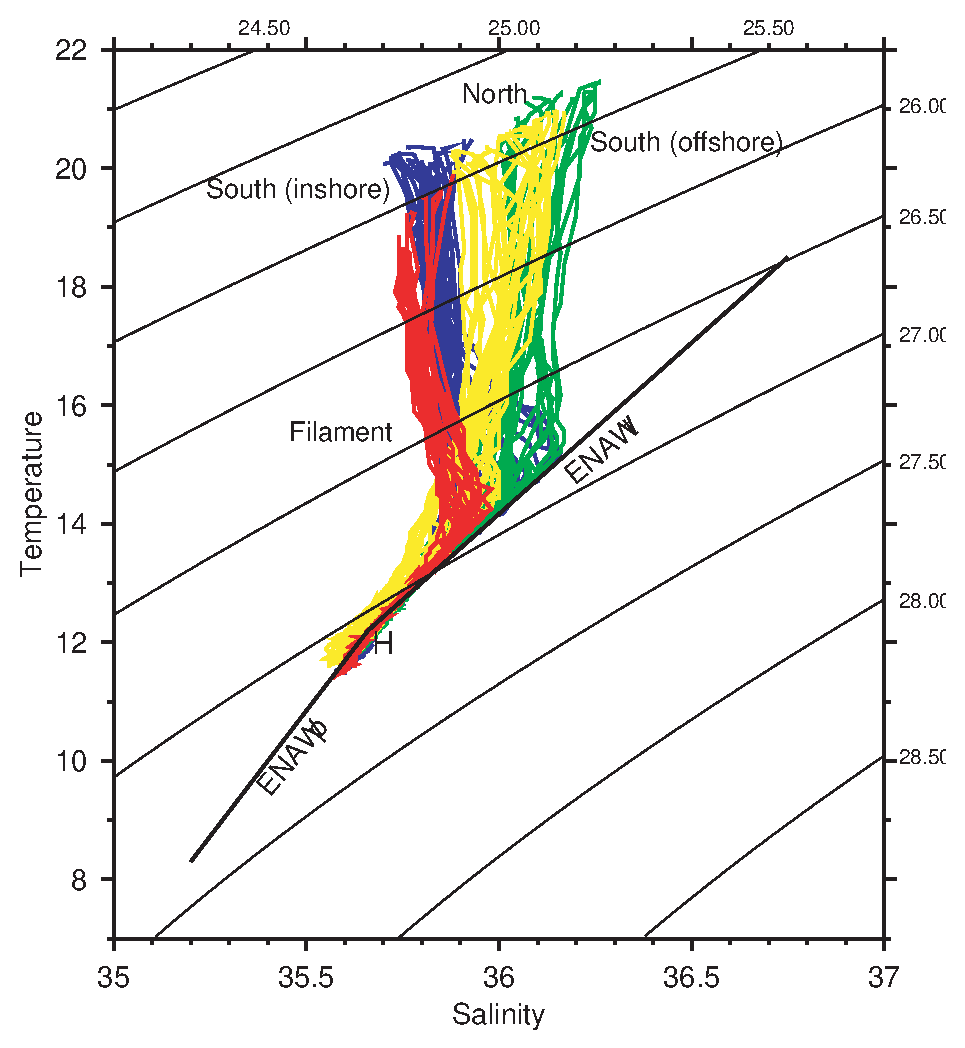
\includegraphics[height=8cm]{ts_diag2}}
   \caption{T/S curves for selected groups of SeaSoar profiles
   between Rias Baixas and southern Portugal revealing the wide
   range of variation alongshore. (a) Characteristic T/S profiles
   of the different upper-layer sub-ambiences likely to be found
   in the Iberian Atlantic coast, (b) strong contrast of the Cape
   Roca filament with respect to surrounding waters. Also shown
   are the characteristic lines of  \enawp and \enawt [{\it Barton
   et al.,} 2002, in preparation].}
  \label{fig:litts}
\end{figure}

The MIW occupies most of the intermediate layer in the Portuguese
coast (Fig.~\ref{fig:ctdmixing}) and is defined by two cores. The
upper core (800m) is characterized by a relative temperature
maximum, 13\deg C, and salinity of 36.4psu,
\citep{Ambar79,Fiuza97} concentrated against the slope in close
relation with the poleward PSU. The MIW lower core (at 1200m) is
better characterized by its salinity maximum, 36.6psu and
temperature of 12.2\deg C \citep{Ambar79}. The lower core is
generally broader and more variable, but on the mid-slope is
strong and persistent \citep{Hamann96}. The MIW is modified along
the Portuguese coast by mixing with the overlying \enaw and so
loses its original characteristics as it progresses northwards
(becoming colder and less saline) until it reaches Cape Finisterre
(43\deg N). There \citet{Rios92} found a strong salinity front,
beyond which the MIW presence was significantly decreased.

In the bottom layer, below 1300m, an isopycnic layer of low
temperature and salinity is commonly found as a result of strong
mixing between the MIW and North Atlantic Deep Water (NADW) on its
way to the south \citep{Ambar94}.

\section{Eastern Boundary Dynamics}\label{sec:upw_theory} Wind-driven
currents are a common feature of the continental shelves and
together with tides they constitute the most energetic,
best-observed and best-modelled form of variability over the
continental margins \citep{Brink98}. In Eastern boundaries,
equatorward winds induce net offshore surface Ekman transport
which brings about transport divergence near the coast and
upwelling of subsurface waters to maintain continuity in the
cross-shelf section. The basic mechanisms of wind-driven coastal
upwelling are well understood and there are several excellent
reviews of upwelling systems \citep[e.g.][]{Allen80,Brink98}.
Other features associated with forcing of finite extent [e.g.
opposing undercurrent and propagation of upwelling by coastal
trapped waves) were reviewed by \citet{Huthnance81} or
\citet{Brink91}. The Californian upwelling system has been the
subject of the most comprehensive and extensive studies such as
CalCOFI, California Cooperative Fisheries Investigations
\citep{Lynn87}, CODE, Coastal Ocean Dynamics Experiment
\citep[e.g.][]{Kosro86}, OPUS, Organization of Persistent
Upwelling Structures, \citep[e.g.][]{Atkinson86} and CTZ, Coastal
Transition Zone \citep{Strub91}, while other Eastern Boundaries
Systems have raised less international attention, e.g. Peru
\citep{Smith81}, NW Africa \citep{Mittelstaed83}, Benguela
Upwelling System \citep{Andrews80} and  West Iberian Peninsula
with the MORENA, Multidisciplinary Oceanographic Research in the
Eastern boundary of the North Atlantic \citep{Fiuza96} and the
recently concluded OMEX II, Ocean Margin Exchanges
\citep{Huthnance02}.

\subsection{Surface Ekman layer}

Currents varying on time-scales of days or longer tend to be
constrained by geostrophy to flow along depth contours. However,
frictional Ekman layers together with local, non-linear and time
dependent flows may relax the geostrophic constraint and
contribute to the ageostrophy of the flow.

The actual contact between wind forcing and the ocean occurs
within the turbulent surface boundary layer, generally called the
Ekman layer. The depth of this layer, typically 10-100m, is
determined by competition between the stabilising effect of
surface heating and the destabilising effects of turbulence
generation by wind input, but also from surface cooling, breaking
waves, or unstable shears in the water column \citep{Brink98}.

Within the surface boundary Ekman layer, the solution to the
governing equations of motion can be found to be a function of the
vertical coordinate only (see \citealp{Pedlosky87} for a full
description of the equations of motion):
\begin{equation}\label{eq:coord}
  u=u(z); v=v(z); w=w(z)
\end{equation}
so that from the continuity equation
\begin{equation}\label{eq:continuity}
  \frac{\partial u}{\partial x}+\frac{\partial v}{\partial y}
  +\frac{\partial w}{\partial z}=0
\end{equation}

we obtained that $\frac{\partial w}{\partial z}=0$. From the
surface boundary condition of $w(0)=0$, it follows that $w$ must
be zero at all depths. The coordinate system adopted is that in
which $x$ is the cross-shelf coordinate (positive onshore), $y$ is
the alongshore coordinate (positive poleward), and $z$ is the
vertical coordinate (positive upward).

Since the fluid is homogeneous, from the hydrostatic approximation
it follows that the horizontal pressure gradient must be
independent of z, and it is therefore entirely determined by any
geostrophic velocity far from the boundary. Ignoring any flows
associated with horizontal pressure gradients is reasonable as
long as the pressure related flow is not too strong; that is, the
(interior) Rossby number
\begin{equation}\label{eq:rossby}
  R_{o}=\frac{v^{*}}{fL}
\end{equation}
(where $v^{*}$ is a typical interior velocity, $f$ is the Coriolis
parameter and $L$ a representative horizontal length scale) is
small.

The basic force balance is then reduced to the local acceleration,
Coriolis and the vertical gradient of turbulent stress. If the
turbulent stress vanishes at some depth below the mixed layer,
then the equations of motion can be vertically integrated to
describe the Ekman transport ($U_{E}$,$V_{E}$):
\begin{equation}\label{eq:ekmanu}
  \frac{\partial U_{E}}{\partial
  t}-fV_{E}=\frac{1}{\rho}\tau_{0}^{x}
\end{equation}
\begin{equation}\label{eq:ekmanv}
  \frac{\partial V_{E}}{\partial
  t}-fU_{E}=\frac{1}{\rho}\tau_{0}^{y}
\end{equation}

where $U_{E}$,$V_{E}$ are the vertically averaged velocities in
the Ekman layer,$\rho$ is the density in the mixed layer and
$\tau_{0}^{x},\tau_{0}^{y}$  are the wind stress applied at the
surface in the $x$ and $y$ directions. Assuming a wind stress of
the form
\begin{equation}\label{eq:windstress}
  \tau_{0}^{y}=T\cos \omega t
\end{equation}

with no component in the across-shelf $(x)$ direction yields a
solution
\begin{equation}\label{eq:ekmansolu}
  U_{E}=\frac{fT}{\rho}(f^{2}-\omega ^{2})^{-1}\cos \omega t
\end{equation}
\begin{equation}\label{eq:ekmansolv}
  V_{E}=\frac{-\omega T}{\rho}(f^{2}-\omega ^{2})^{-1}\sin \omega t
\end{equation}

where $T$ and $\omega$  are the amplitude and frequency of the
wind stress. In the low frequency limit ($f\gg \omega $),
rotational effects dominate and the Ekman transport is
perpendicular to the wind stress. In the high frequency limit
($f\ll \omega$ ), the transport is downwind but lags by a quarter
cycle.
\begin{figure}
  \centering
  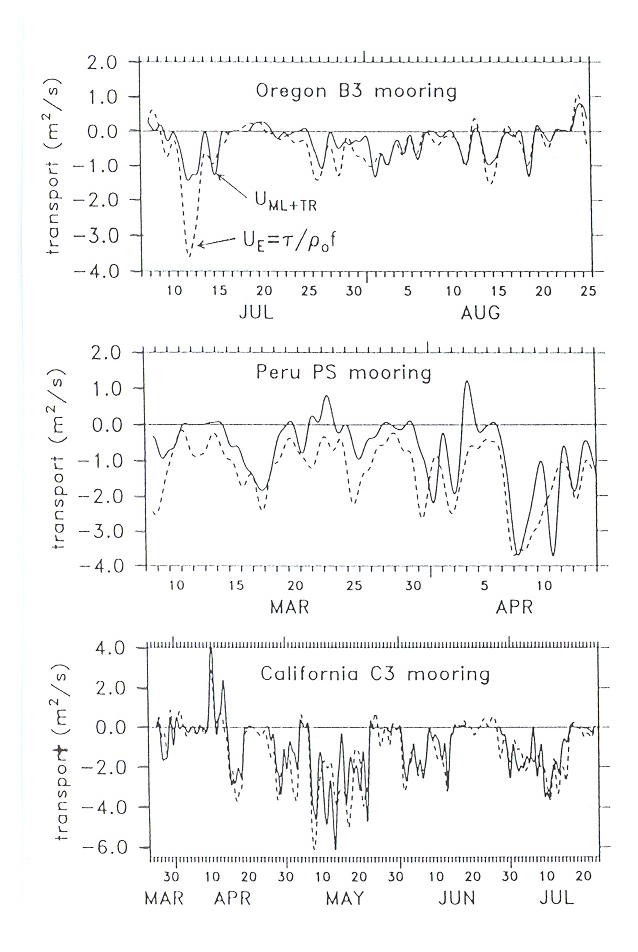
\includegraphics[height=9cm]{fig14new}
  \caption{Time series of cross-shelf transport in the surface
  boundary layer $U(ML+TL)$ (Mixed + Transitional Layer, solid line)
  and the Ekman transport $U_E=\frac{\tau}{(\rho f)}$ (dashed line) from three locations
  during the upwelling season of 1982 [{\it Lentz} 1992].}
  \label{fig:ekmanlayer}
\end{figure}

\begin{figure}
  \centering
  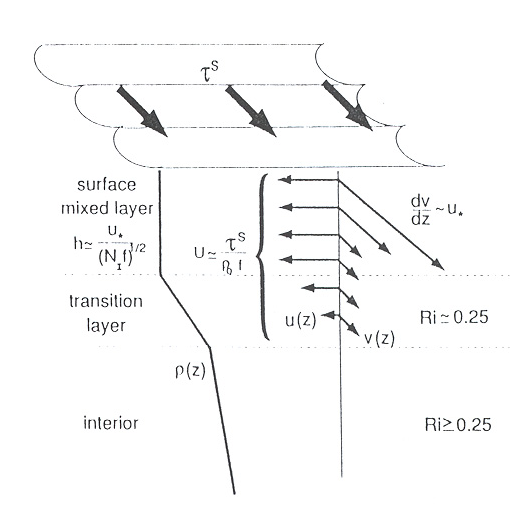
\includegraphics[height=9cm]{fig15new}
  \caption{Schematic summarizing some of the characteristics of
  the surface boundary layer in a coastal upwelling region:
  $u^*=(\frac{\tau^{s}}{\rho_0})^{\frac{1}{2}}$ is the shear
  velocity and $U$ is the cross-shelf transport in the surface
  mixed layer plus the transition layer [{\it Lentz} 1992].}
  \label{fig:upperlayerdiag}
\end{figure}
In most cases, the low frequency limit is an adequate description
which basically reduces eq.~\ref{eq:ekmansolu},~\ref{eq:ekmansolv}
to the theoretical Ekman transport $(\rho f)^{-1}\tau_{0}^{y}$,
which is completely determined in terms of the local value of the
$y$-component of the wind stress. Substantial effort has been
directed towards the verification of the theoretical Ekman
transport \citep{Smith81,Brink83}, especially in coastal upwelling
regions. \citet{Lentz92} reported experiments in 4 coastal
upwelling regions which demonstrated good agreement in magnitude
and variability between the observed cross-shelf Ekman transport
and the theoretical value (Fig.~\ref{fig:ekmanlayer}) but only
when he allowed for the surface Ekman layer being about 25-50\%
deeper than the surface mixed layer including a transitional
stratified layer of near critical Richardson number ($\sim$0.25).
The subtidal surface mixed layer depth was found to be well
described in terms of the wind-induced shear velocity
($u_*=(\frac{\tau_0^y}{\rho_0})$) , the Coriolis parameter ($f$)
and the buoyancy frequency below the mixed layer ($N_I$) in the
form
\begin{equation}\label{eq:ekmandepth}
  \delta _E=\frac{u_*}{(N_If)^{\frac{1}{2}}}
\end{equation}

It was found no account need be made for the surface heat flux and
heat advection as they tend to balance each other in the coastal
upwelling regions studied. Fig.~\ref{fig:upperlayerdiag} shows an
schematic of the upper water column geometry in coastal upwelling
systems.

Secondary pressure related flows can become important and
influence Ekman layer processes. Vorticity of the background flow
allows convergences and divergences in the Ekman transport even
under the effects of a uniform wind \citep{Niiler69}.
\subsubsection{Coastal wind-driven upwelling}
In a coastal context, wind-driven flows can be described by
depth-integrated equations of motion where nonlinearities and
density variations are not allowed:
\begin{equation}\label{eq:winddriven1}
  \frac{\partial U}{\partial t}-fV=-\frac{1}{\rho}h\frac{\partial
  p}{\partial x}+\frac{1}{\rho}(\tau_0^x-\tau_B^x)
\end{equation}
\begin{equation}\label{eq:winddriven2}
   \frac{\partial V}{\partial t}-fU=-\frac{1}{\rho}h\frac{\partial
  p}{\partial y}+\frac{1}{\rho}(\tau_0^y-\tau_B^y)
\end{equation}
\begin{equation}\label{eq:winddriven3}
\frac{\partial U}{\partial x}+\frac{\partial V}{\partial y}=0
\end{equation}

where $U,V$ are the cross-shore and along-shore depth-integrated
transports, $h(x)$ is the water depth and p is the pressure. A
rigid lid is assumed for the surface boundary because interest is
confined to relatively short spatial scales compared to the
barotropic radius of deformation (natural horizontal scale for
upwelling and expected distance from the coast of the upwelling
front). The bottom stress will be assumed to be proportional to
the depth-averaged current,
\begin{equation}\label{eq:botstress1}
\tau_B^x=\rho rh^{-1}U
\end{equation}
\begin{equation}\label{eq:botstress2}
\tau_B^y=\rho rh^{-1}V
\end{equation}

where $r$ is the drag coefficient.

Solving eq.~\ref{eq:winddriven1},~\ref{eq:winddriven2} and
~\ref{eq:winddriven3} is easier if the long-wave approximation is
made. This assumes that alongshore scales are large relative to
cross-shelf scales, ($Ly \gg Lx$) , time scales of interest are
long relative to the inertial period, ($f \gg \omega$)(more
specifically, longer than the sum of the inertial period and the
frictional e-folding time dependent on the depth \citep{Dalu90})
and finally that frictional effects are not too large ($f\gg
rh^{-1}$). This approximation is justifiable as the major
upwelling systems are induced by large scale wind patterns
characterised by alongshore spatial scales larger than the
shelf-slope width and weather changes do occur at time scales
longer than  several days.

\begin{figure}
  \centering
  \includegraphics[height=9cm]{fig16a}
  \includegraphics[height=9cm]{fig16b}
  \caption{Aircraft wind measurements acquired during CODE 2
  experiment (summer 1982) from which (1) wind stress (Pa) and (2)
  wind stress curl (Pa/100km) were computed. (3) and (4) show
  simulations from a simple, two layer, vertically integrated
  model of coastal upwelling. They represent the upper-layer
  thickness (in m) after 24 hours of simulation using observed
  wind stresses, (3) without curl and (4) with curl. Note how the
  nonzero stress curl enhanced coastal upwelling, the greatest
  effects being around the areas of largest observed curl values
  [{\it Enriquez and Friehe}, 1995].}
  \label{fig:capewind}
\end{figure}


The long-wave approximation has as a main consequence that
alongshore flows are stronger than cross-shelf flows which is a
common characteristic of upwelling systems
\citep[e.g.][]{Batteen97}, and that the alongshore flow is in
geostrophic balance due to the scaling of eq.~\ref{eq:winddriven1}
(cross-shelf wind and bottom stress and local cross-shelf
acceleration can be neglected relative to the Coriolis and
pressure terms):
\begin{equation}\label{eq:geost}
  -fV=-\frac{1h}{\rho}\frac{\partial p}{\partial x}
\end{equation}
The main failure of the scaling approximation resides in the
alongshore uniformity of the wind and topography. It is well
established that coastal irregularities such as capes or bays may
induce wind stress variations (Fig.~\ref{fig:capewind}) which are
of major importance in the evolution and final equilibrium state
of upwelling systems \citep[e.g.][]{Haynes93,Enriquez95}.
Furthermore, lateral wind stress gradients can induce Ekman
pumping and enhance the baroclinicity of the alongshore flow
\citep{Brink87,Batteen92}.

Nevertheless the above simplified model can be solved for a
spatially uniform constant alongshore wind $\tau_0^y=T$, with no
alongshore variations allowed,$\frac{\partial}{\partial y}=0$ so
that continuity reduces to
\begin{equation}\label{eq:consimp}
 \frac{\partial U}{\partial x}=0
\end{equation}
On the coastal boundary the no cross-shelf flow must applied so
that the depth-integrated cross-shelf transport must vanish
everywhere, which reduces eq.~\ref{eq:winddriven2} to
\begin{eqnarray}\label{eq:depthmotion}
 &U=-\frac{1}{f}\frac{\partial V}{\partial t}+
 \frac{1}{\rho f}\tau_0^y-\frac{rV}{fh}=0  \\
 & \equiv U_I+U_{E0}+U_{EB}=0 \nonumber
\end{eqnarray}
where $U_I$ is the interior transport, $U_{E0}$ is the surface
Ekman transport and $U_{EB}$ is the bottom Ekman transport.
Basically, the surface Ekman flow is compensated by flows deeper
in the water column sufficiently far from the coastal boundary
where lateral friction and vertical velocities can not be
neglected. Solving eq.~\ref{eq:depthmotion} for $V$ is
straightforward in a system starting from the rest, i.e. $V=0$ at
$t=0$:
\begin{equation}\label{eq:depthsol1}
  V=\frac{hT}{r\rho}[1-\exp(-rh^{-1}t)]
\end{equation}
\begin{figure}
  \centering
  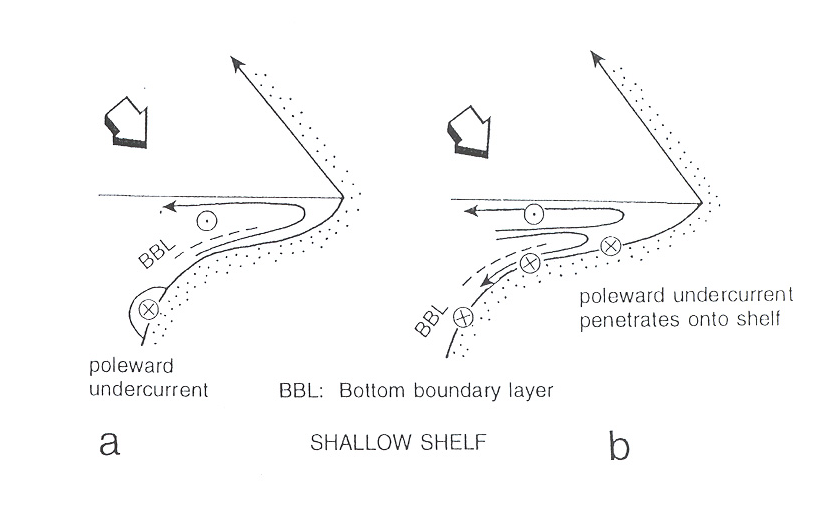
\includegraphics[height=8cm]{fig18new}
  \caption{Schematic of coastal upwelling: (a) upwelling over a
  shallow frictional shelf where the equatorward flow on the shelf
  penetrates to the bottom and bottom Ekman transport is onshore,
  supplying the upwelling waters; (b) upwelling over a shallow
  frictional shelf when the poleward undercurrent penetrates the
  shelf and the bottom Ekman layer transport is offshore and
  upwelling water are supplied from middepth
  [{\it Hill et al.,}, 1998].}
  \label{fig:polewdiag}
\end{figure}

It can be seen that for $t \ll rh^{-1}$ the alongshore flow
accelerates steadily at a rate,
\begin{equation}\label{eq:depthsol2}
  V\approx \frac{T}{\rho}t
\end{equation}
so that the surface Ekman flow is compensated mainly from the
interior flow. At larger times, $t \gg rh^{-1}$, the interior flow
disappears $(\frac{\partial V}{\partial t}=0)$ reaching a steady
state and the surface Ekman flow is now compensated entirely by
the bottom Ekman flow, i.e. the flow is entirely frictional
determined (Fig.~\ref{fig:polewdiag}). More generally, however,
this equilibrium is not reached; acceleration, stratification and
the ignored along-shore pressure gradients also distribute the
stress and upwelling through the water column \citep{Huthnance95}.

Upwelling systems are generally highly time-dependent and respond
rapidly to wind stress fluctuations. Initially the upwelling
favourable winds drive an offshore Ekman flow which forces the
interface (seasonal thermocline) beneath the upper layer to rise
near the coast at a distance defined by the Rossby radius of
deformation,$R'=\frac{HN}{f}$ where $H$ is the depth of the mixed
surface layer, usually taken to be the same as the surface Ekman
layer, and $N$ is the buoyancy frequency below the mixed layer,
generating geostrophically balanced alongshore currents, namely an
equatorward coastal jet and a poleward undercurrent. The upwelled
water band width,$R'$, will be also governed by the time
integrated offshore Ekman transport , so that the band tends to be
narrower where the upwelling-favorable winds are intermittent
(e.g. Oregon) and broader where winds are steadier and stronger
(e.g. California) \citep{Szoeke84}. Sufficiently far
$(>\frac{HN}{f})$ from the coast the inflow is uniform through
depth without a vertical component, as described by
eq.~\ref{eq:depthmotion}. In the presence of stratification, an
upper layer of characteristics $H_1N_1$ over a $2^{nd}$ layer of
$H_2N_2 (H_1N_1 > H_2N_2)$ gives a majority of upwelling inflow in
the upper layer within $(>\frac{H_1N_1}{f})$ of the coast. The
magnitude of the alongshore current in the coastal jet and the
horizontal scale of the coastal jet also depend on stratification
increasing as $N^2$ increases, whereas weaker stratification
enables the front to develop faster \citep{Allen95}.

The time evolution of the system will also be affected by
diffusive processes induced by upwelling and mixing, which reduce
the coastal layer depth and density stratification  $(H_1N_1)$ and
hence the offshore scale \citep{Szoeke84}. One non-linear aspect
of the system is that the front and surface jet are advected
offshore by Ekman drift although they will be generally limited to
the shelf, stopping at any shelf break \citep{Huthnance95}. The
absence of a front over the shelf has been related to sustained
favourable upwelling winds, for example in Peru (15\deg S) or off
central California \citep{Smith81,Brink83}.
\begin{figure}
  \centering
  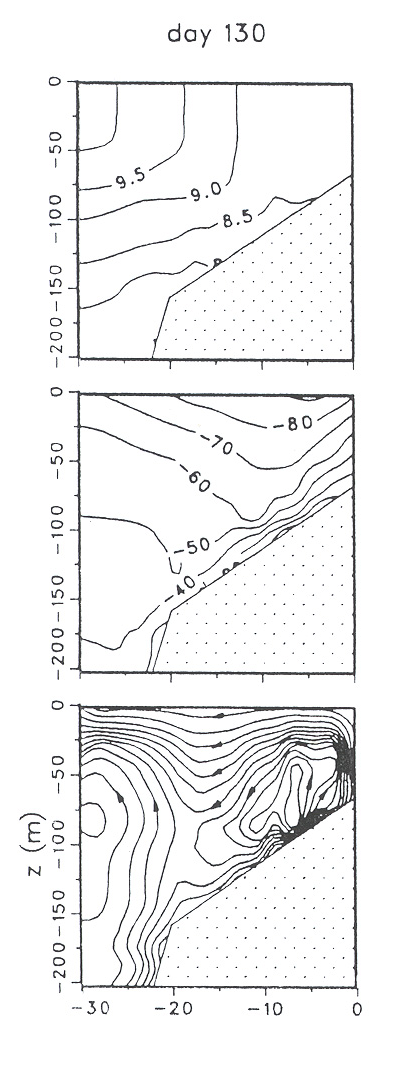
\includegraphics[height=12cm]{fig17new}
  \caption{Prediction from a combined two-dimensional circulation
  model and one dimensional mixed-layer model of cross-shelf
  structures of Temperature ($C$)(top), alongshore velocity
  (\velc)(middle), and stream function (\mixc)(bottom). On day 130
  the equatorward wind stress is the strongest and the upwelling
  front moves to the outer shelf. Upwelling takes place in two
  narrow areas, one at the coast and the other on the seaward side
  of the front. In association with the convergence and divergence
  of the upper layer transport, a prominent double-cell
  circulation is formed
  [{\it Chen and Wang,}, 1990].}
  \label{fig:cellcirc}
\end{figure}

The front itself is characterised by relatively large horizontal
density and alongshore velocity $(v)$ gradient near surface and
large vertical gradients in $v$ at mid-depth. There is
occasionally a convergence of near-surface offshore flow at the
front that results in a general increase in depth of the surface
turbulent boundary layer across the front \citep{Allen95} and that
has been suggested to constitute a two cell pattern
(Fig.~\ref{fig:cellcirc}) \citep{Chen90}. In response to strong
winds the front would display a tendency for the surface isotherms
to parallel the bottom topography as a result of advection by a
nearly uniform Ekman transport while weaker winds produce a
complex contouring front \citep{Brink83}.

A large variety of studies acknowledges the important role of
shelf/slope topography in upwelling, a factor which has been
neglected to this point in the review. Complex coastal features
such as capes, ridges, submarine canyons and submarine banks,
which have along-shelf scales that are comparable to or smaller
than cross-shelf scales produce flow structures that differ
fundamentally from those addressed by the classical theory and are
often the site of significant cross-isobath flows
\citep{Trowbridge98}.

The classical assumption of an along-shelf length scale much
larger than the cross-shelf length scale leads to an along-shelf
flow which is nearly geostrophic even when the Rossby $(R_0)$ and
vertical Ekman numbers ($E_v=\frac{A_v}{fH^2}$  where $A_v$ is the
vertical mixing coefficient assumed independent of $z$, and $H$ is
a typical vertical scale ) approach unity as shown by the scaling
of the momentum equations \citep{Trowbridge98}. The geostrophic
balance is only slightly altered by changes in the cross-shelf
velocity caused by ageostrophic processes (mixing and local
acceleration). On the other hand, the cross-shelf velocity is
likely to be ageostrophic even when the Rossby and Ekman numbers
are small, so that small changes in the along-shelf velocity have
a major impact on the cross-shelf flow.

Another source of time dependence in upwelling systems is brought
about by propagation of disturbances from remote locations by
coastally trapped waves (see later) which induce variability on
time scales of from 3 to 10 days \citep{Denbo87}.
Fig.~\ref{fig:3dupwdiag} shows an schematic of the common features
that can be expected in a coastal upwelling system.
\begin{figure}
  \centering
  \includegraphics[height=13cm]{upwfig}
  \caption{Schematic of an upwelling system showing the varied
  range of possible physical processes and the complex 3
  dimensionality of the system
  [{\it Hill et al.,}, 1998].}
  \label{fig:3dupwdiag}
\end{figure}

Most coastal upwelling is produced by along-shelf wind stresses
and may be altered greatly by short along-shelf scales in the
coastline \citep{Crepon82,Crepon84,Haynes93,Wang97} in turn
altering the local direction of the wind relative to the coastline
and reducing or enhancing upwelling/downwelling locally.
Consequently, along-shelf variations in the pressure gradient will
be introduced, which may then propagate along the coast as CTW's
\citep{Crepon82} and give rise to a countercurrent below the
thermocline opposing the prevailing winds \citep{Suginohara82}.

\citet{Enriquez95} showed that the wind small-scale spatial
variability near Pt. Arena (California) had characteristic scales
much smaller than the scales of synoptic atmospheric pressure
patterns and calculated local wind stress curl five times larger
than those obtained from long-term ship data using bulk
aerodynamic formulas. The local coastline (cape) was responsible
for a sustained curl pattern which modified the dynamical response
of the coastal water to the applied wind stress and resulted in
local enhancement of upwelling downwind of the cape during
favourable winds (Fig.~\ref{fig:capewind}). The theoretical study
of \citet{Crepon84} also supports upwelling enhancement downwind
of a cape relating the intensity to the offshore scale of the cape
while the geometry of the cape does not change the process
qualitatively. The cape, like the alongshore variability in the
wind-stress, generates an undercurrent in the opposite direction
to the wind.

The shelf geometry itself also influences the upwelling system.
Shallow wide shelves without poleward undercurrent generate large
bottom friction and larger Ekman onshore transport which in turn
limits the acceleration of the jet so weaker surface jets are
expected. The front is wider and occurs further offshore
\citep{Allen95}. The concentration of depth contours tends to
guide and strengthen currents along the continental slope where
the sea floor slope exerts an stabilising effect
\citep{Huthnance81}. In those steep shelves, the vertical
gradients of v tend to be more geostrophically balanced so that
the frictional bottom boundary layer is weaker and carries less
fraction of onshore flow. Near-surface density gradients tend to
occur near the coast so that offshore-displaced upwelling fronts
may not be observed. \citep{Allen95}.

\subsection{Instabilities}

Mathematical models investigating the dynamics of upwelling,
filaments, squirts and eddies suggest that the phenomena result
from instability of alongshore currents, and they all point toward
baroclinic instability as being an important process. Several of
this models also developed small-scale disturbances along fronts
and indicated that other instability mechanisms are involved in
their generation as well \citep{McCreary91}. In those mathematical
models, meanders and eddies increased in scale as the system
adjusted toward equilibrium, apparently for different dynamical
reasons in each case.

\citet{McCreary91} reviewed previous stability models and
experimented with simpler models to infer two types of
instability, as also found by \citet{Barth94} with continuous
forms of stratification and coastal current. These two
instabilities are: shorter-scale frontal instability depending on
gradients of sea-surface temperature, trapped to the front and
upper column and extracting potential energy; a larger-scale
``traditional'' baroclinic instability manifested later in
filament development. The vertical shear between an equatorward
upwelling front jet and the poleward undercurrent give a mechanism
for the generation of baroclinic instabilities as shown by model
experiments in the Californian shelf by \citet{Batteen89}.

\subsection{Coastal trapped waves}
The sudden change in bathymetry at the shelf-edge imply a large
potential vorticity gradient and provide conditions that lead to
the trapping of certain wave motions called continental shelf
waves or coastal trapped waves \citep{Huthnance81}. These waves
are commonly generated by transient winds \citep{Adams69} and
propagate along the shelf-edge, cyclonically around the ocean at
sub-inertial frequencies \citep{Huthnance86}. They arise from the
conservation of potential vorticity as water passes over uneven
bottom topography:
\begin{equation}\label{eq:ctw}
  \frac{d(\frac{f+\xi}{h})}{dt}=0
\end{equation}

According to eq.~\ref{eq:ctw}, if a fluid column is displaced up
or down a slope, vortex stretching or compression will tend to
move the water back to where it was originally. This results in
long, sub-inertial wave forms which propagate cyclonically in the
northern hemisphere, with the shallow water on their right. They
tend to decay off-shelf but some may be at their most energetic
over the slope \citep{Huthnance95}.

A numerical investigation by \citet{Suginohara74,Suginohara82} of
a coastal ocean with cross-shelf topography and vertical
stratification underlies the importance of coastal trapped waves
in the development of an upwelling circulation including that of a
poleward flow of about 2\velc. \citet{Denbo87} and others, have
shown the importance of Coastal trapped waves in wind-driven
currents in the CODE area.

\subsection{Poleward slope flow}
Current along the continental slope can and do occur with non-zero
time-average and velocities exceeding or opposing those to either
side of the adjacent shelf and ocean \citep{Huthnance95}. Poleward
slope currents are in fact widespread in Eastern boundaries, and
often flow against prevailing equatorward winds as in seasonal
upwelling systems (e.g. California) , which suggests a
large-scale, non-local forcing of the current. The precise
cross-shelf distribution of the flow depends upon the character of
the forcing balanced by alongshore pressure gradient, friction and
acceleration.

The steep topography of the slope and the influence of Earth's
rotation are the primary factors aligning barotropic currents
along the depth contours and both continuity arguments and
potential vorticity conservation can explain the anchorage of the
slope current along the slope region. Usually the poleward flow is
located at the shelf break or over the continental slope with a
width of the order of 20-100km and current speeds of order of
10\velc.

The several potential forcing forces are:
\begin{itemize}
  \item Freshwater runoff resulting in a baroclinic coastal current
\citep{Hill98} which can include the shelf edge for sufficient
runoff and narrow shelf.
  \item Alongshore pressure gradients imposed by the ocean and
incorporating density forcing combined with the slope bathymetry
to drive the slope poleward current.
\end{itemize}

The latter one is of most general ubiquity and was described by
\citet{Huthnance84}. It was termed JEBAR, Joint Effect of
Baroclinicity And Relief, and refers to the dynamical adjustment
of the density-induced pressure gradient to the bottom slope when
the zonally orientated density surfaces intersects a meridional
sloping boundary (Fig.~\ref{fig:jebar}). Under no net cross-shore
transport and assuming the same meridional density gradient is
affecting both the shelf and the ocean, the alongshore sea-level
slope is proportional to the bottom depth. On the shelf the
sea-level drop is less than in the ocean then generating an
offshore pressure gradient which drives the poleward flow along
the slope. This pressure gradient increases along-slope therefore
accelerating the flow until friction becomes important and a
steady state is reached.
\begin{figure}
  \centering
  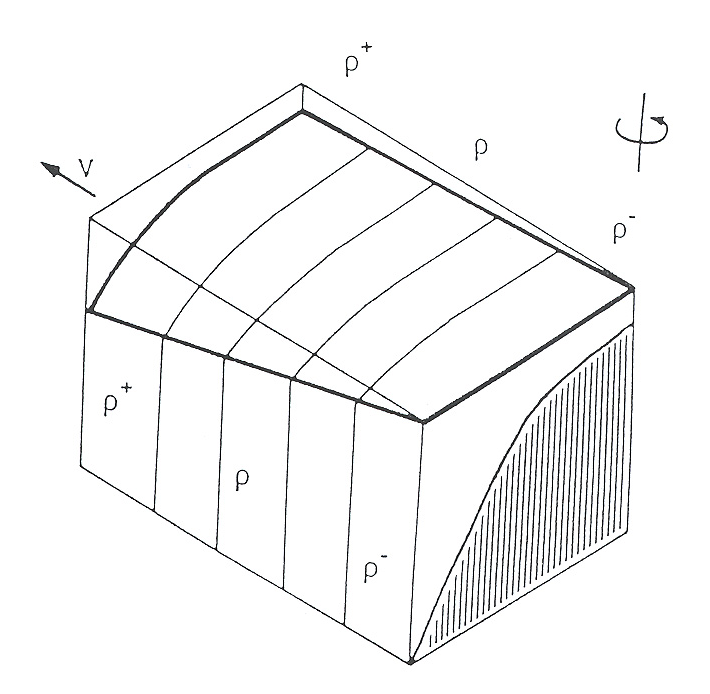
\includegraphics[height=8cm]{fig20new}
  \caption{A simple JEBAR model. The sea surface over a
  shelf-slope region is shown as a thick line. Density increases
  alongshore and continuity is maintained by a condition of no net
  cross-slope transport. Sea level declines more gently over
  shallow water than over deep water hence a steepening
  cross-slope sea level difference develops which drives a
  strengthening along-slope current
  [{\it Hill,}, 1998].}
  \label{fig:jebar}
\end{figure}


In upwelling systems, there also exist local terms forcing the
poleward undercurrent which are highly influenced by alongshore
variability \citep{Hill98}. Some of these possible forcings for
undercurrent poleward flow in the face of equatorward wind stress
are: remote forcing, relaxation of equatorward wind, the positive
curl of equatorward wind stress or thermohaline forcing
\citep{McCreary87}. Along-slope variations in topography could
allow the necessary alongshore pressure gradient to drive the
undercurrent as alongshore variations in the wind stress field
would do too \citep{Hill98}. There are multiple observational
evidences of the poleward undercurrent in the Oregon upwelling
system but only scattered ones in the Eastern Atlantic coast like
N.West Africa where the poleward undercurrent flows below the
shelf break \citep{Mittelstaed75,Barton90} and on the Portuguese
slope where six month long measurements of poleward flow were
recorded by \citet{Ambar84,Ambar85} at levels below 200m in bottom
depth less than 1000m. Off Oregon the shelf break is less sharp
and so the undercurrent is partly on the shelf \citep{Huyer76}.

%
\graphicspath{{d:/papers/qscatwind/graphics/}}
\chapter{Winds}\label{ch:winds}
\section{Introduction}
In Eastern Upwelling systems, coastal winds are the major forcing
in the residual circulation and largely determine the seasonality
of the region. The time scales of the wind forcing are typically
of the order of a few days to weeks superimposed on a slowly
varying seasonal signal. The seasonal signal influences the
residual circulation and thereby the basin scale response.

The coast of Galicia (Spain, Iberia peninsula) constitutes the
northern limit of the North Atlantic Upwelling regime, which
extends from 44\deg to almost 10\deg N south of Dakar. During the
summer months, when the Azores high-pressure cell is in the
central North Atlantic and the Greenland low is weak, the
resulting pressure gradient drives the trade wind southward along
the coast of Iberia inducing upwelling and associated southward
currents. In the winter months, when the Azores high is located
further south off NW Africa, and the Greenland low is deep and
located off southeastern Greenland, the pressure gradient between
the two pressure systems results in an onshore and slightly
northward wind off Iberia, and downwelling.

The summer upwelling regime in the Galician coast is highly
variable in time and spatially complex; the upper layer responds
to rapid wind stress changes in 3 or fewer days
\citep{Mcclain86,Huthnance02}. Some of the complexity can be
related to the irregular coastline, where Cape Finisterre marks
the abrupt change between the meridional west and the zonal north
coasts of Galicia. Capes or bays may induce important wind stress
variations \citep{Enriquez95}, sometimes accelerating the flow to
become supercritical \citep{Winant88}. Its kinetic energy is then
trapped to produce localized upwelling maxima and upwelling
filaments e.g. Pt. Conception, California \citep{Barth87}.

Finisterre is frequently the site of a stationary upwelling
maximum \citep{Blanton84,Castro94} and a recurrent upwelling
filament \citep{Haynes93}. The authors found good agreement
between the laboratory results of \citet{Narimousa89} and spatial
structure of filaments in the Portuguese and Spanish Atlantic
coast and concluded that major capes in the region played an
important role in filament formation. They suggested however that
the filament near Finisterre was an ``overshoot'' of the coastal
jet when upwelling occurs along the northern coast.
\citet{Mcclain86} noted that different wind directions resulted in
upwelling either north or south of Finisterre but not usually
both.

The winter onshore wind regime is marked by the formation of a
narrow, warm and salty surface poleward current along the Iberian
Atlantic continental slope \citep{Frouin90,Haynes90}, which
settles in November and disappears around May. Two main mechanisms
have been proposed to drive the poleward flow: wind-stress and
thermohaline forcing. \citet{Frouin90} concluded that wind stress
could account for only one fifth of the total poleward transport
and considered the thermohaline forcing to be the main driving
mechanism. The latter is associated with the large scale
meridional pressure gradient in the upper 200-300m caused by the
poleward temperature decrease and the slope bathymetry
\citep{Huthnance95}. The large scale pressure gradient is a
consistent feature and interannual variations of the poleward flow
could be related to anomalous winds.

Although the wind field plays a major role in the Galician region,
it has largely been studied superficially in terms of upwelling
indices estimated from geostrophic winds calculated for a cell
centered offshore Finisterre. Large scale studies by
\citet{Bakun91} and \citet{Wooster76} have demonstrated the
important seasonal variability of wind stress and wind stress
curl, but were based on seasonally averaged winds at wide spacing.
Only the temporal variability at a few coastal sites has been
related with upwelling processes. For example, \citet{Fiuza82b}
showed the seasonal and interannual dependence of coastal
upwelling on coastal winds at Portuguese sites. In the present
chapter 2 years of wind data from the QuikScat mission are
analysed, supplemented by {\it in situ} observations at near-shore
buoys, in relation to AVHRR sea-surface temperatures. First,
seasonal differences and typical wind patterns are described.
Different coherent wind patterns lead to formation of the
Finisterre filament and cause the differences in the upwelling
north and south of the cape seen in SST images. Spatial wind
patterns related to the larger scale pressure fields are used to
explain variations between different upwelling years. The winter
wind regime is described during both an ``anomalous'' and a
``typical'' year and the implications of the wind patterns in the
evolution of the upwelling and non-upwelling regimes are
discussed.

\section{Methods}
\label{metodos}  The SeaWinds instrument on the QuikScat satellite
is a specialized microwave radar that, since 21 July 1999, has
measured near surface wind speed and direction twice daily in
1,800 km swath bands. Wind speed measurements range from 3 to 20
m/s, with an accuracy of 2 m/s and 20$^{\circ}$ in direction.
Spatial resolution of 25 km enables identification of fine scale
features poorly sampled with previous scatterometers. The small
coast mask makes the data suitable for studying near-shore wind
patterns and processes.

Wind data were retrieved from the Jet Propulsion Laboratory web
site [{\it http://podaac.\\
jpl.nasa.gov/quikscat/qscat\_data.html}] as Level
3 Scientific product. The data set consists of global gridded
values of meridional and zonal components of wind velocity on an
approximately 0.25 x 0.25 degree grid. The data were obtained from
the Direction Interval Retrieval with Threshold Nudging (DIRTH)
wind vector solutions contained in the QuikScat Level 2B data.

The data from either the ascending pass (6AM LST equator crossing)
or the descending pass (6PM LST equator crossing) were selected
each day from 19 July 1999 to 16 May 2001, depending on which had
the higher data density. The data cover the Coastal Transition
Zone off Galicia, 40.5$^{\circ}$N to 45.5$^{\circ}$N and
6.5$^{\circ}$W to 13$^{\circ}$W. Gaps in the data were dealt with
by objectively interpolating the data. This method is equivalent
to applying a spatial filter with smoothing scales 0.25$^{\circ}$
(0.55$^{\circ}$) in longitude (latitude).

\begin{figure}
\centering
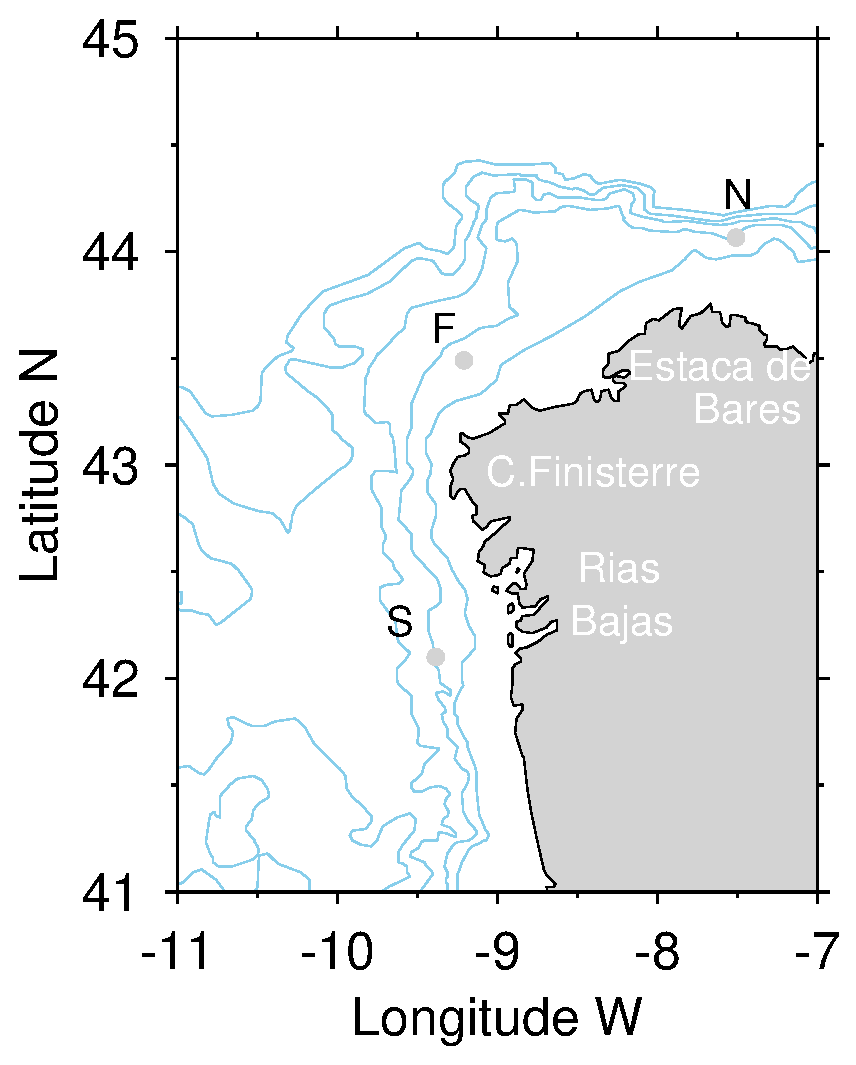
\includegraphics[height=7cm,keepaspectratio=true]{coast}
\caption{Map of the region of study with the position of the main
coastline features and instruments. }\label{fig:ib}
\end{figure}

The remotely sensed wind data were complemented with a set of {\it
in situ} wind observations collected between 1 May and 15 August
1999 by 3 buoys from the Spanish agency {\it Puertos del Estado}
Deep Water Network (DWN), moored near the Galician shelf break
(Fig.~\ref{fig:ib}). They were located at 44\deg~3.9'N,
7\deg~31.1'W in 382m north of Finisterre (Estaca de Bares); at
43\deg~29.4'N, 9\deg~12.6'W in 382m off cape Finisterre
(Villano-Sisargas) and at 42\deg~6'N, 9\deg~23.2'W in 323m
(Silleiro). In the text we refer to them as N, F and S buoys,
respectively. The DWN buoys also measured currents at 3m depth by
an UCM60 acoustic currentmeter. The data were measured hourly and
filtered with a moving average filter A24A24A25 \citep{Godin91}
with a cutoff frequency of 30 hours to remove tides and inertial
components.

SST from Advanced Very High Resolution Radiometer (AVHRR) for the
same period and location were processed at Plymouth Marine
Laboratory using the Panorama software \citep{Miller97} .

Wind data were further processed by calculating Complex Empirical
Orthogonal functions (CEOFs) similar to \citet{Munchow00}. CEOFs
provide an objective means to summarize the wind measurements and
to establish the dominant mesoscale features coherent within the
data set.

The wind data are expressed in a two dimensional complex vector
where the $u$ component is the real part and $v$ the imaginary
part (Eq.~\ref{wind}) and $X_{i}(i=1\ldots N)$ denote the location
and $t_{k}(k=1\ldots M)$ time.
\begin{equation}\label{wind}
  W(X_{i},t_{k})=u(X_{i},t_{k})+\hat{\i}v(X_{i},t_{k})
\end{equation}
In matrix form it is,
\[W=\left(
\begin{array}{ccc}\label{matrix}
  W_{1}(1) & \ldots & W_{1}(N) \\
  \vdots & \ddots & \vdots \\
  W_{M}(1) & \ldots & W_{M}(N)
\end{array} \right).\]
For each data series the temporal mean was subtracted and the
modified covariance matrix $R$ calculated,
\begin{equation}\label{cov}
R=W\times W^{*}/(M-1),
\end{equation}
where the $^{*}$ denotes the complex conjugate and results in a
$M\times M$ matrix. We have normally dealt with matrices
containing more locations than points in time (N$>$M),which
results in a smaller matrix than the true covariance matrix. The
CEOFs are obtained by solving,
\begin{equation}\label{eigs}
  R\times D=D\times \Lambda,
\end{equation}
where $\Lambda$ are the real eigenvalues of the covariance matrix,
which are identical irrespective of which way the covariance is
calculated \citep{Kelly88}. $D$ are the complex eigenvectors which
are different from the results we would have obtained using an
$N\times N$ covariance matrix but they can be calculated from,
\begin{equation}\label{recon}
  E=W^{*}\times D,
\end{equation}
by which we obtained $E$, an $N\times M$ matrix. Therefore we
calculate a smaller number of eigenvectors than the $N$
eigenvectors that are defined for the problem but, because only
the first few are significant, the lost ones are irrelevant.

The time varying amplitudes are obtained as shown in
Eq.~\ref{amp},
\begin{equation}\label{amp}
  A=W\times E,
\end{equation}
where $A$ is complex, having magnitude and orientation, and
represents the amplification factors for the spatial patterns. The
original data can be reconstructed from,
\begin{equation}\label{orig}
F=A\times E^{*}.
\end{equation}

The orientation of the temporal amplitudes and spatial patterns
are relative to an arbitrary reference \citep{Kundu76}. To
facilitate their interpretation the spatial patterns and temporal
amplitudes are rotated along the direction of the semimajor
principal axis of the corresponding amplitude time series
\citep{Merrifield89}. Furthermore, the amplitude and spatial modes
are normalized in such a way that amplitude series have uniform
variance, and the spatial modes have units of m/s and correspond
to a vertical amplitude of value 1.

Two important properties of EOFs are that the spatial
distributions are orthogonal and that their time series are
uncorrelated over the data set. Thus the EOFs are uncorrelated
modes of variability. Usually a large portion of the variance can
be explained by a small number of modes. To decide which modes are
significant the sampling error associated with the EOF analysis
was estimated following the method described by \citet{North82},
\begin{equation}\label{eq1}
  \delta \lambda_i = \lambda_i \left(\frac{2}{n} \right)^{1/2},
\end{equation}
where $\delta \lambda_i$ refers to the sampling error of the ith
mode, $\lambda_i$ is the ith eigenvalue, and n, the number of
independent measurements or degrees of freedom, is calculated
after \citet{Davies76}, according to
\begin{equation}\label{eq2}
  n=\frac{N\Delta t}{\tau}.
\end{equation}
Here, $\Delta t$ is the sampling interval, $N$ is the number of
records, and $\tau$ a de-correlation timescale,
\begin{equation}\label{eq3}
  \tau = \sum_{i=-\infty}^{\infty} C_{uu}(i\Delta t) C_{vv}(i\Delta
  t)\Delta t.
\end{equation}
$C_{uu}(t)$ and $C_{vv}(t)$ are the lagged autocorrelation
functions of $U(t)$ and $V(t)$ series. The sampling errors
associated with each eigenvalue of the first 6 eigenfunctions are
computed using equations \ref{eq1} to \ref{eq3}. Only those
eigenmodes whose errors do not overlap are distinct.


\section{Seasonal evolution of the Galician region}
\begin{figure}[t]
\noindent
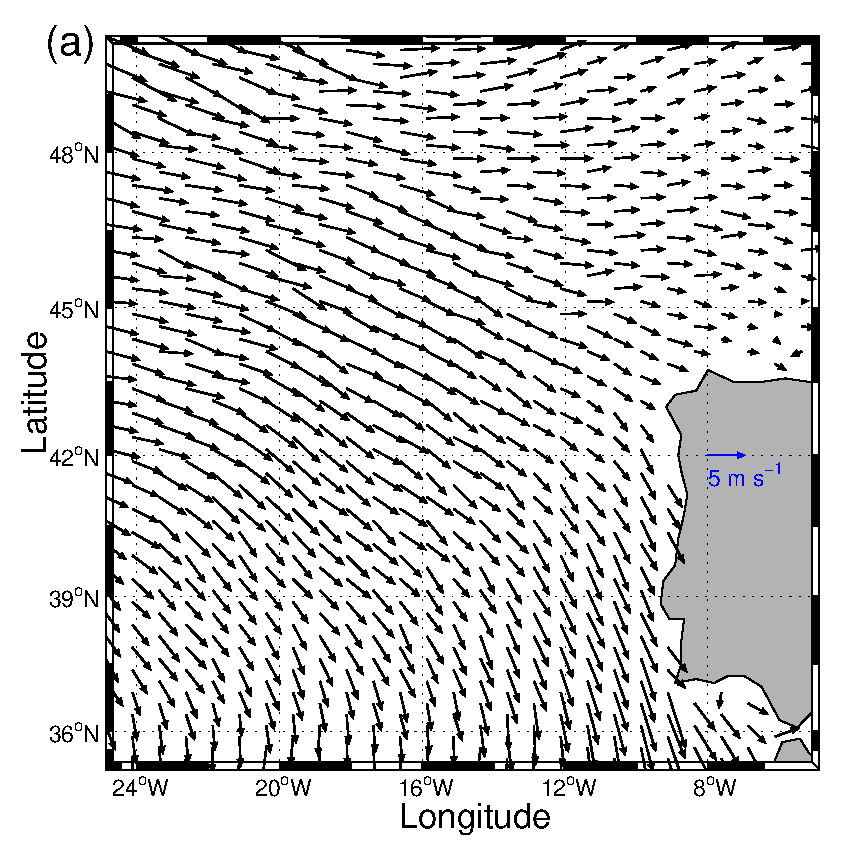
\includegraphics[height=7cm]{summer_median99}
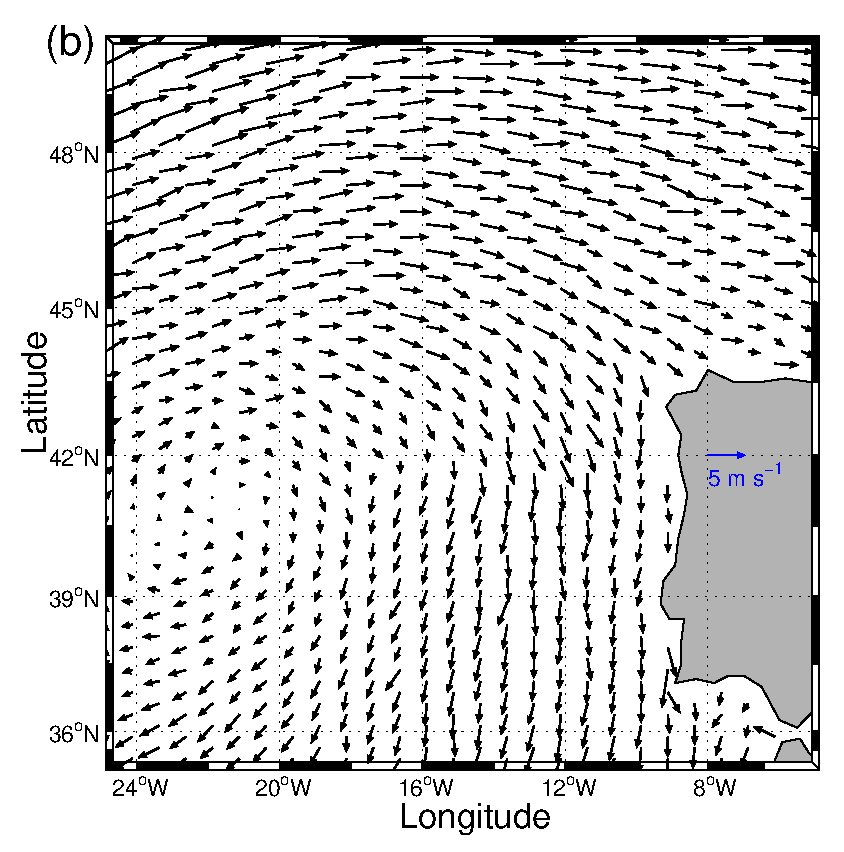
\includegraphics[height=7cm]{winter_median99}
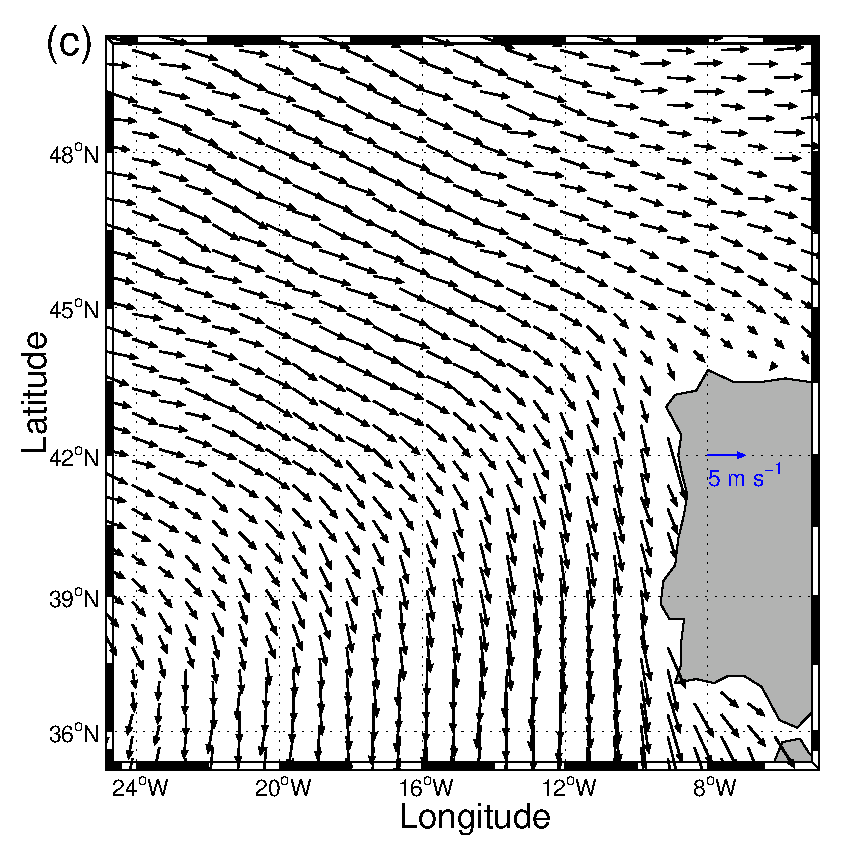
\includegraphics[height=7cm]{summer_median00}
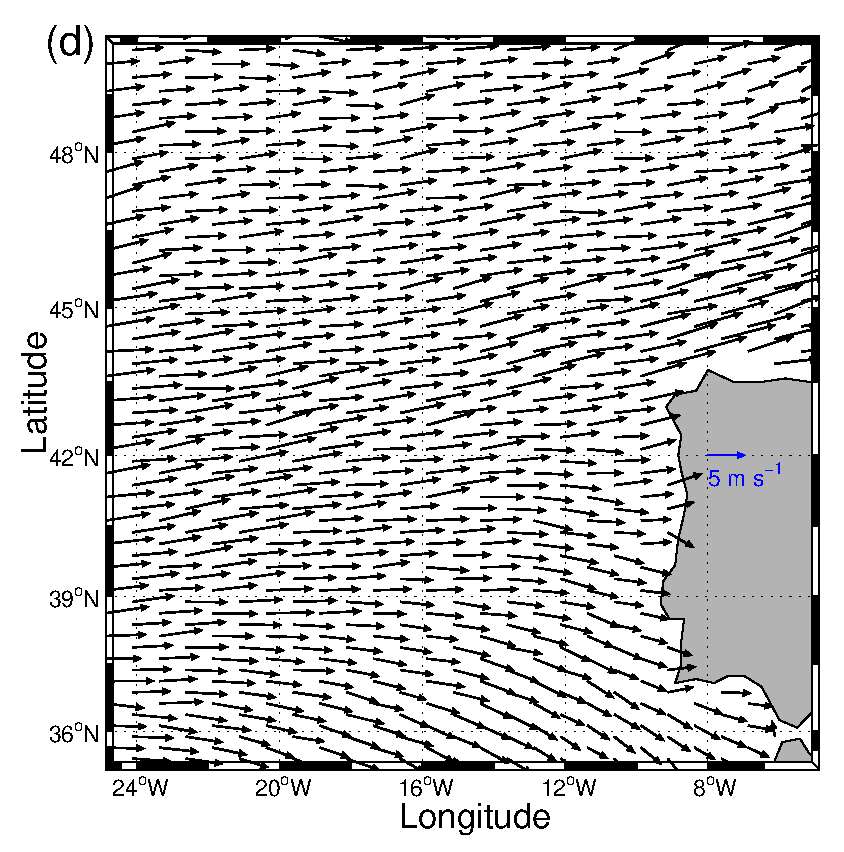
\includegraphics[height=7cm]{winter_median00}
\caption{Median wind fields from (a) summer 1999 (July-October),
(b) winter 1999 (November-April), (c) summer 2000 (May-October)
and (d) winter 2000 (November-April)}\label{fig:windsmedian}
\end{figure}
The seasonal wind regime in the Iberian peninsula can be broadly
divided into summer upwelling and winter downwelling regimes. The
median of the wind field for summers 1999 and 2000 in
{Fig~\ref{fig:windsmedian}}a and c, shows typical upwelling
favorable winds along the Atlantic coast of Galicia strengthening
to the south. North of Cape Finisterre the winds are locally
downwelling favorable flowing to the south-west. The typical
downwelling winter regime is characterized by onshore winds on the
Atlantic coast as in winter 2000-2001
(Fig~\ref{fig:windsmedian}d). This picture is however complicated
by interannual variations in the location of the pressure systems
(Fig~\ref{fig:windsmedian}b), as occurred in winter 1999-2000. The
Azores high remained in a more northern location than winter
2000-2001 and the median of the winds show a large scale
circulation like the summers of 1999 and 2000
(Fig~\ref{fig:windsmedian}a and 1c) albeit with weaker winds.
\begin{figure}
\subfigure[June\,20-26\,1999]
{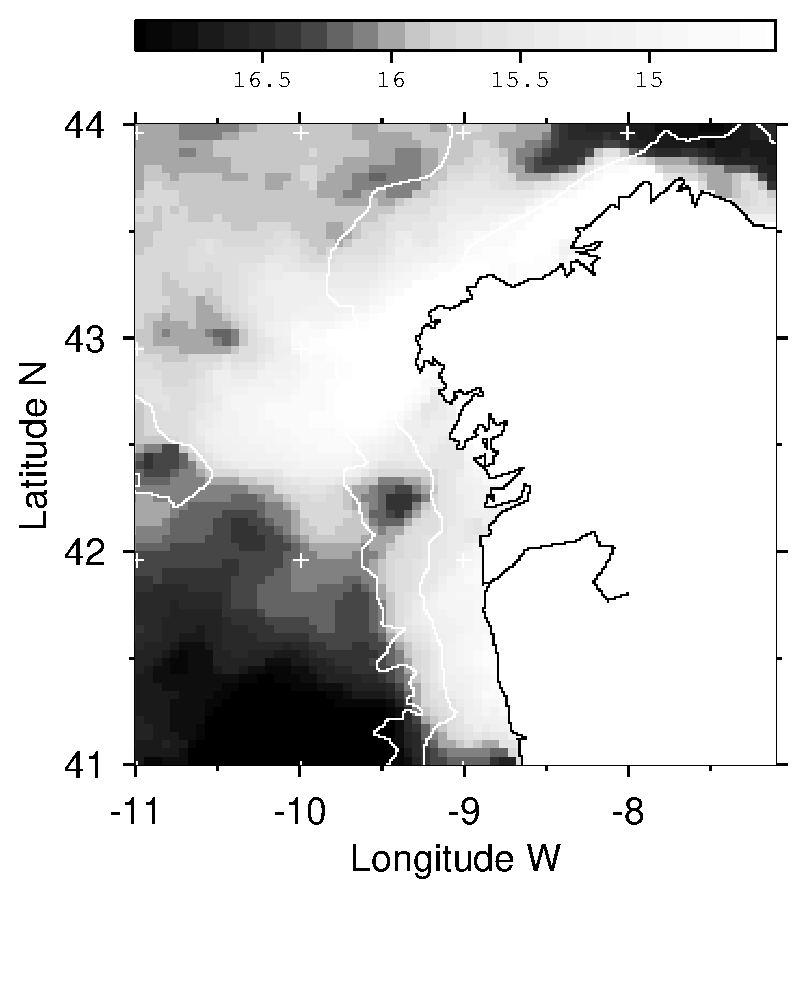
\includegraphics[height=5.3cm]{ga990620-0626medfincolphd}}%
\subfigure[Aug 15-21 1999]
{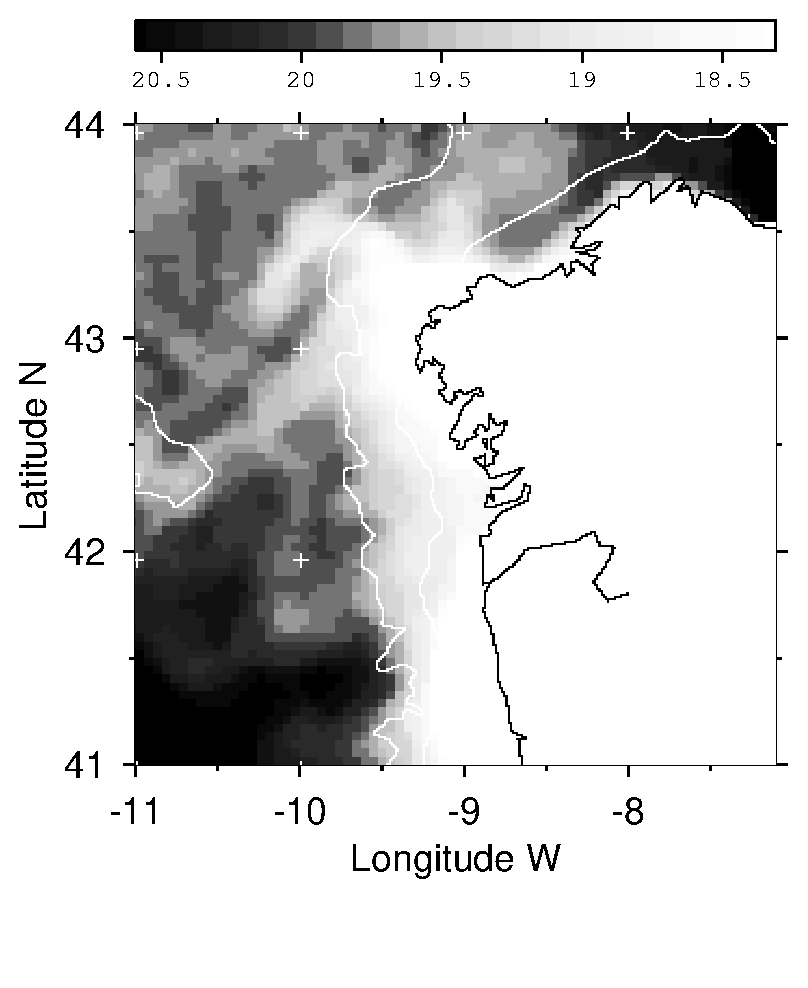
\includegraphics[height=5.3cm]{ga990815-0821medfincolphd}}%
\subfigure[\mbox{Nov\,7-13\,1999}]
{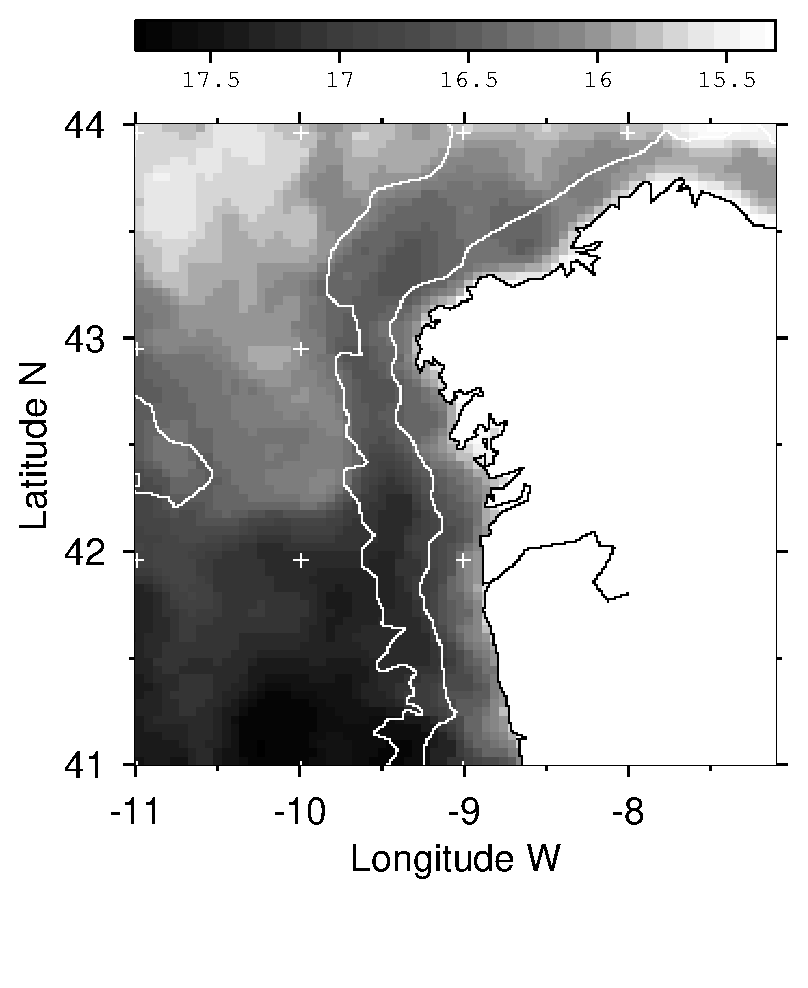
\includegraphics[height=5.3cm]{ga991107-1113medfincolphd}}
\subfigure[May 21-27 2000]
{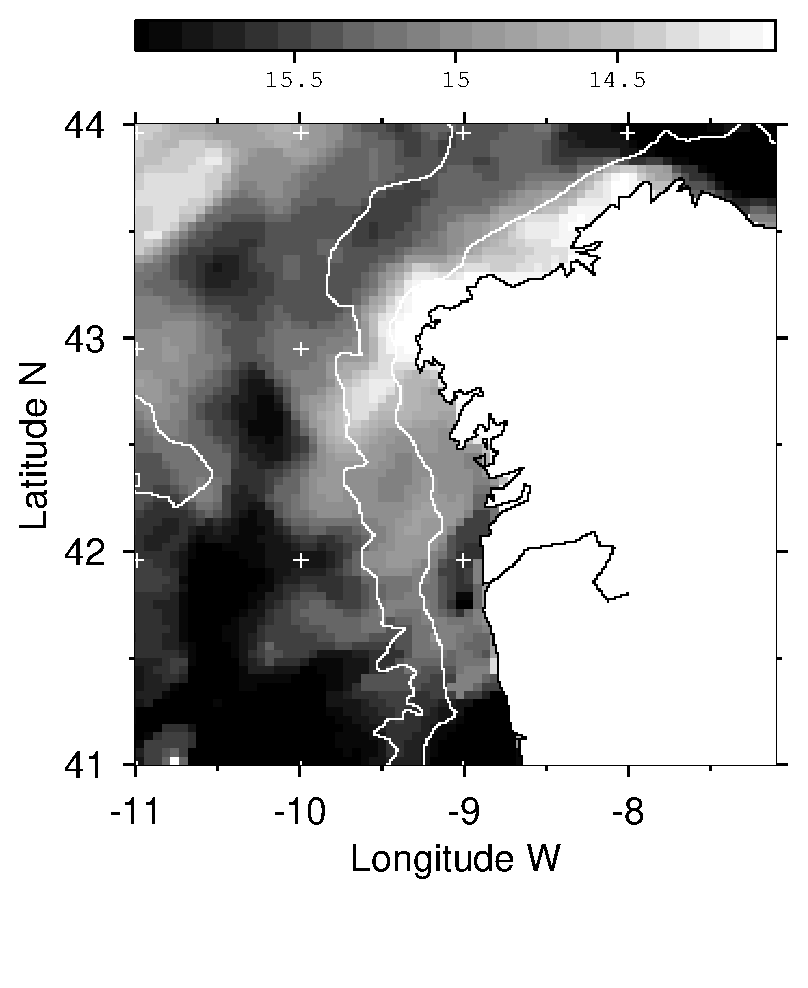
\includegraphics[height=5.3cm]{ga000521-0527medfincolphd}}%
\subfigure[\mbox{Jul\,16-22\,2000}]
{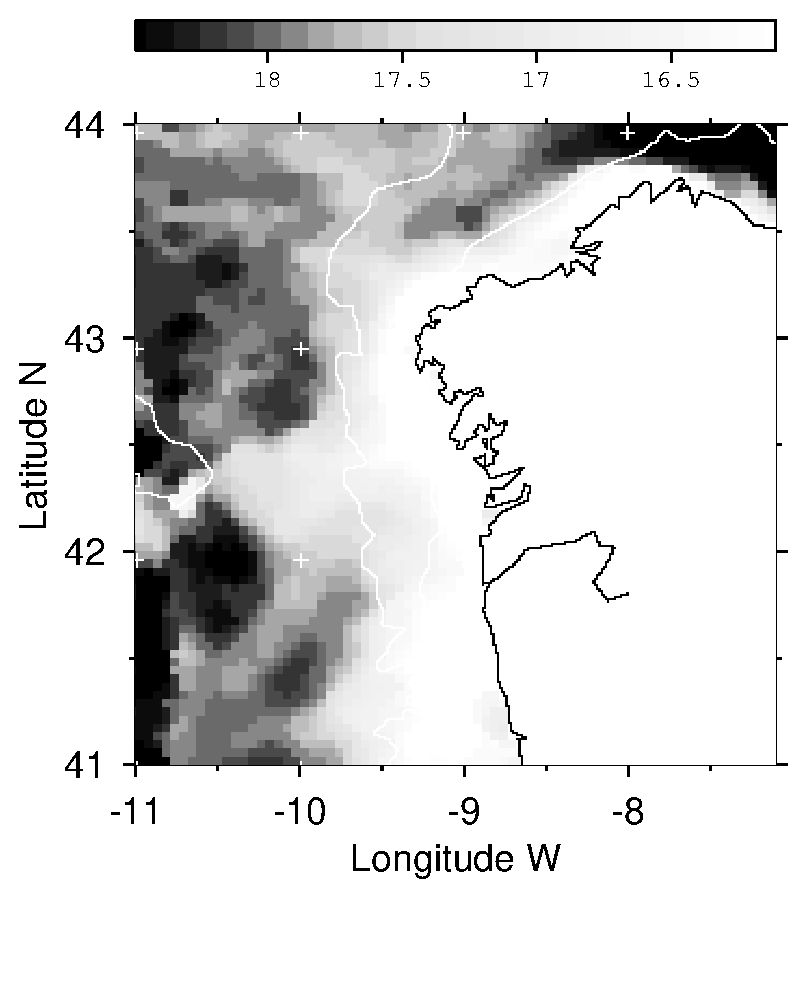
\includegraphics[height=5.3cm]{ga000716-0722medfincolphd}}%
\subfigure[Mar 11-17 2001]
{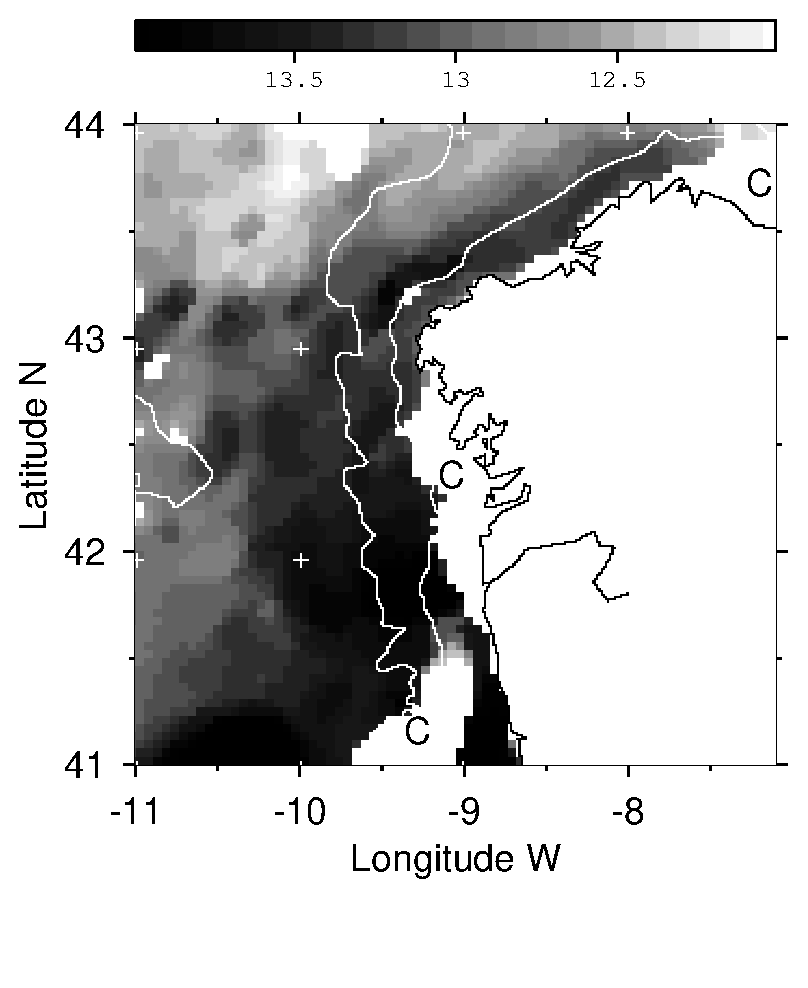
\includegraphics[height=5.3cm]{ga010311-0317medfinphd}}
\caption{Samples of weekly SST average images for the period of
study. Note the different temperature scales.}
\label{fig:windssstsummary}
\end{figure}

Partly in response to the annual winds the coastal regime
typically changes from upwelling in summer to downwelling and
slope poleward flow in winter, as in the period of study,
1999-2001, ({Fig~\ref{fig:windssstsummary}}). During both summers
upwelling took place from June-October. The first sign of
upwelling in 1999 started to appear in early June as a cold thin
strip next to the Atlantic coast off Galicia. By mid June
(Fig~\ref{fig:windssstsummary}a), the upwelling was stronger in
the north coast and the Finisterre filament was starting to
develop. The Finisterre filament was present for most of June and
July and disappeared in August (Fig~\ref{fig:windssstsummary}b).
No other filament developed during this season. This is not
exceptional in the Galician region. Years 1995 and 1996 (not
shown) also saw a predominance of north coast upwelling and the
Finisterre filament over other filaments. Examination of weekly
composites of SST imagery for the period 1993-2000 suggests that
the Finisterre filament is normally the first one to appear and is
accompanied by north coast upwelling.

Poleward flow, suggested in SST by a warm tongue extending along
the shelf break (Fig~\ref{fig:windssstsummary}c), started to
develop from the 20 October and persisted till early May.  Several
periods of weakened (end November) or absent (March) warm anomaly
suggest suppression of the poleward flow.

Upwelling in 2000 started earlier, the first signs appearing in
mid-May north of Cape Finisterre. At the same time the Finisterre
filament started to develop (Fig~\ref{fig:windssstsummary}d)
although it disappeared at the end of May, and never reached the
size of the previous year. Upwelling occurred intermittently until
mid-July (Fig~\ref{fig:windssstsummary}e), then almost
continuously for the rest of the season but no clear filament
developed at the Cape. Moreover, north of Finisterre upwelling was
very weak while to the south, upwelling extended beyond the 200m
isobath with intermittent filament formation. The insignificant
filament activity was compensated by an upwelling season extending
to mid-November.

Poleward flow in the following season was first seen in early
December 2000 and lasted until late April. Its SST signal in March
(Fig.~\ref{fig:windssstsummary}f) shows a narrow extension of
warmer water turning east around cape Finisterre along the
northern coast.

\begin{figure}
\centering \noindent
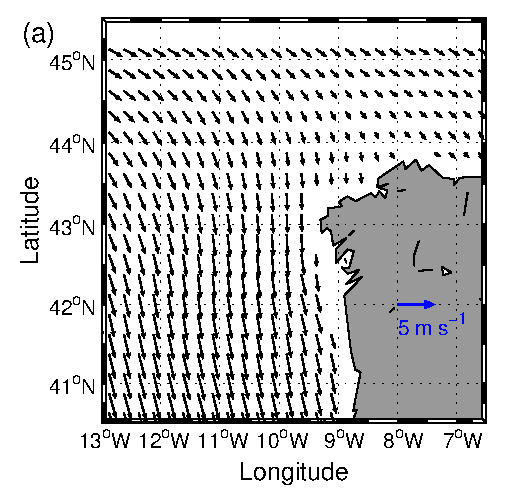
\includegraphics[height=8cm,keepaspectratio=true]{99-00complex_mean}\quad
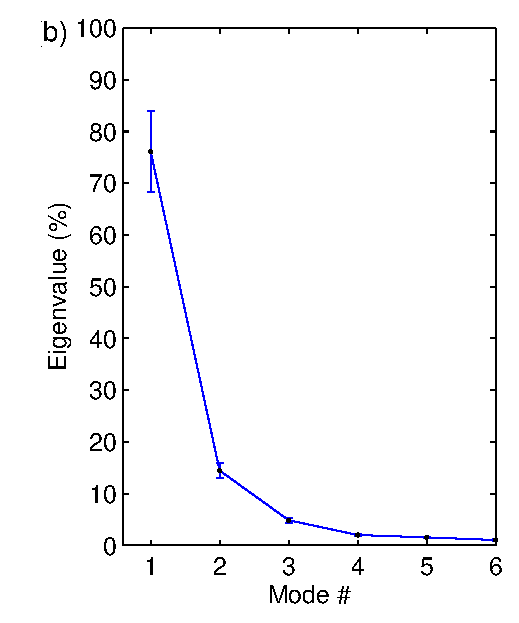
\includegraphics[height=8cm,keepaspectratio=true]{99-00complex_var}
\caption{Mean and variance distribution from the seasonal EOF
analysis, 13  October 1999 to 28 October 2000
}\label{fig:windsmeanvar}
\end{figure}
\section{Common spatial wind patterns}
A CEOF analysis was performed on the 2 year record comprising both
upwelling and non-upwelling regimes. Further CEOF analysis of
shorter data periods to investigate regime or interannual
differences showed a high consistency in the spatial modes and
variance distribution with the full record analysis. Figures
\ref{fig:windsmeanvar} and \ref{fig:windseofseasonal} show the
overall representative results. The mean wind field
(Fig~\ref{fig:windsmeanvar}a), subtracted from the data prior to
the EOF calculations, resembles the median
(Fig~\ref{fig:windsmedian}a and b). The first two modes account
for 88\% of the total variance (Fig~\ref{fig:windsmeanvar}b) and
are statistically distinct since the uncertainty of the
eigenvalues do not overlap with any of the other eigenvalues
\nocite{north82}[\markcite{{\it North et al.,} 1982}]. The
de-correlation time scale for all QuikScat data was shorter than 2
days and a conservative value of 3 days was used in all
uncertainty estimates.
\begin{figure}
\centering
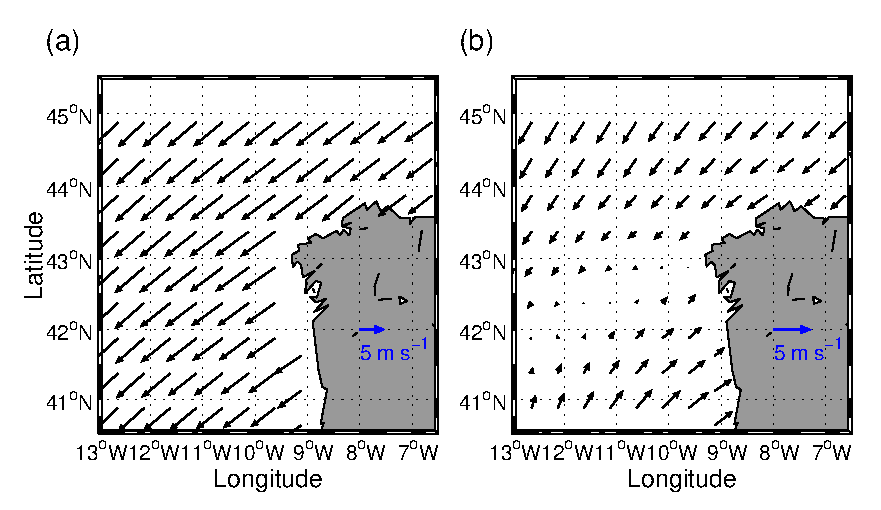
\includegraphics[height=8cm,keepaspectratio=true]{99-00complex_eof12}
\caption{EOF wind distinctive modes from the seasonal analysis (13
October 1999 to 28 October 2000), First a), Second
a).}\label{fig:windseofseasonal}
\end{figure}

Figure~\ref{fig:windseofseasonal} depicts the spatial pattern of
the largest 2 modes. The first mode
({Fig~\ref{fig:windseofseasonal}}a), corresponding to a spatially
coherent wind field, represented 74\% of the total variance.  The
second mode (14\% of total variance), where the wind field is
opposed in direction north and south of Finisterre, adds wind curl
to the first mode  (Fig~\ref{fig:windseofseasonal}b). The mode
shows a minimum of wind speed and maximum wind curl along a line
running south-west from Finisterre with a uniform intensification
to the north and strengthening near the coast to the south. This
mode would contribute to Ekman pumping along the line of minimum
wind intensity.
\begin{figure}[t]
\centering
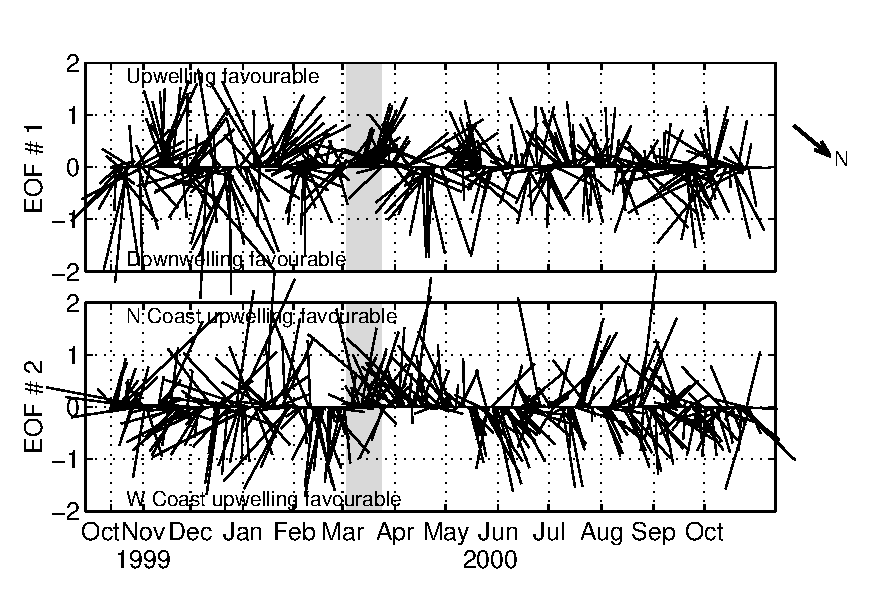
\includegraphics[height=9cm,keepaspectratio=true]{99-00amplitudes}
\caption{Amplitude Time series for the seasonal analysis (13
October 1999 to 28 October 2000). The shaded intervals are
referred to in the text. The arrow on the left points at the
geographical North for the largely coherent wind field of Mode
1.}\label{fig:windsampseasonal}
\end{figure}
\subsection{The 1999-2000 season} The instantaneous orientation
depends on the direction of the complex amplitudes. The patterns
shown in Fig~\ref{fig:windseofseasonal} correspond to a unit
amplitude vector in the direction of the principal axis which is
represented in {Fig~\ref{fig:windsampseasonal}} by a unit vector
pointing vertically upwards. A unit vector to the right represents
the same pattern rotated 90\deg clockwise. For clarity, the
direction of southerly winds is represented by the arrow to the
right of Fig~\ref{fig:windsampseasonal}a. The amplitude time
series for mode 1(Fig~\ref{fig:windsampseasonal}a) is highly
variable for the period 13 Oct 1999 to 28 Oct 2000 comprising one
upwelling/non-upwelling cycle as identified from SST imagery. The
large scale wind is far from unidirectional and changes occur very
rapidly, as the short de-correlation time suggests. For this year,
the expected seasonal signal is absent although both upwelling and
downwelling events were stronger in winter than in summer, in
particular from October to January. The downwelling events,
lasting for about 4-5 days, alternated with longer and more
consistent upwelling events. Nonetheless, downwelling was
predominant during October, December and April.
\begin{figure}
\centering
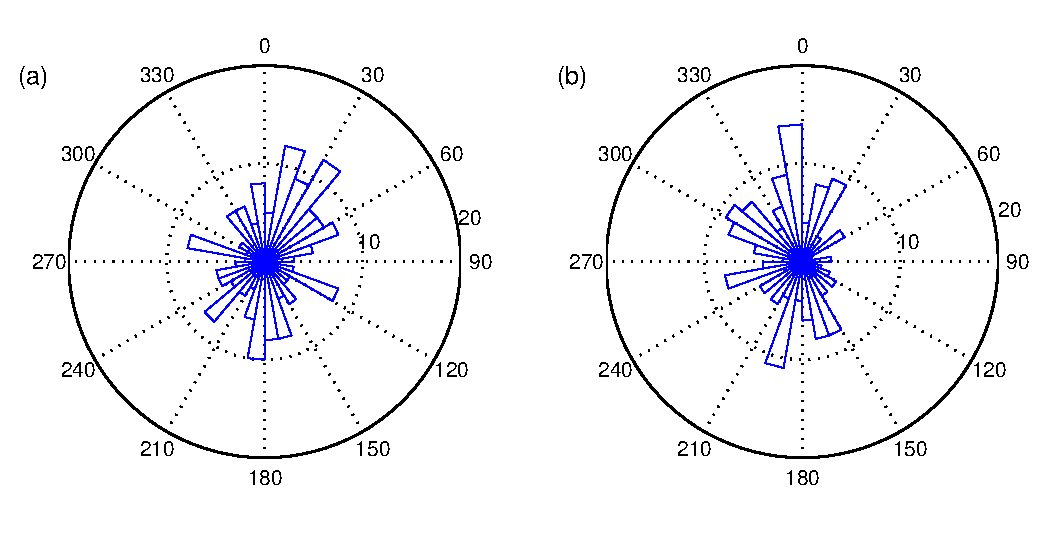
\includegraphics[height=6cm,keepaspectratio=true]{99-00amplitudes_rose_s_w}
\caption{Rose plot of EOF \#1 amplitude directions for winter
(Oct-April) and summer (May-Oct)
1999-2000.}\label{fig:windsroseeof1}
\end{figure}

Directional differences in the wind occur between summer and
winter. During winter ({Fig~\ref{fig:windsroseeof1}}a) there are
two main orientations, the first corresponds to that shown in
Fig~\ref{fig:windseofseasonal}a, rotated 10-40\deg clockwise.
Adding the mean field makes the wind south of Finisterre more
aligned with the coast. The second preferred orientation
corresponds to the less common downwelling winds, i.e., rotated
160-190\deg to the pattern of Fig.~\ref{fig:windseofseasonal}a. In
summer (Fig~\ref{fig:windsroseeof1}b) the preferred orientation
corresponds to the pattern shown in
Fig~\ref{fig:windseofseasonal}a (i.e. no rotation), while other
maxima correspond to the orientations already discussed for the
winter period and 290-320\deg, an enhancement of the mean field.
\begin{figure}[t]
\centering
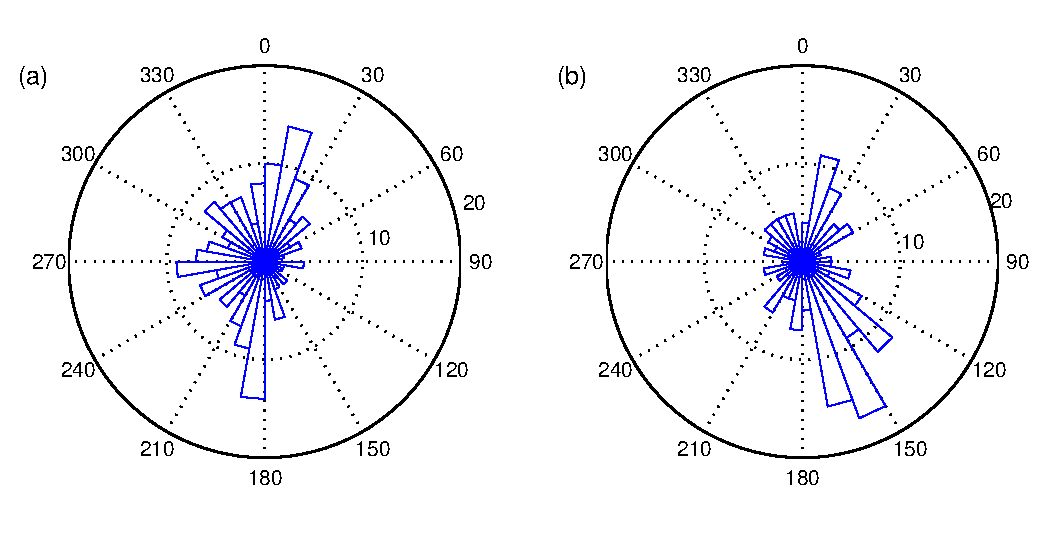
\includegraphics[height=6cm,keepaspectratio=true]{99-00amplitudes_rose_s_w_pc_2}
\caption{Rose plot of EOF \#2 directions for winter (Oct-April)
and summer (May-Oct) 1999-2000.}\label{fig:windsroseeof2}
\end{figure}

In winter, mode 2 ({Fig~\ref{fig:windsroseeof2}}a) shows similar
orientations to mode 1 (between 0-30\deg and 180-210\deg). During
summer, orientations between 130-170\deg were dominant with a
small contribution from 10-30\deg (Fig~\ref{fig:windsroseeof2}b).

\begin{figure}
\centering
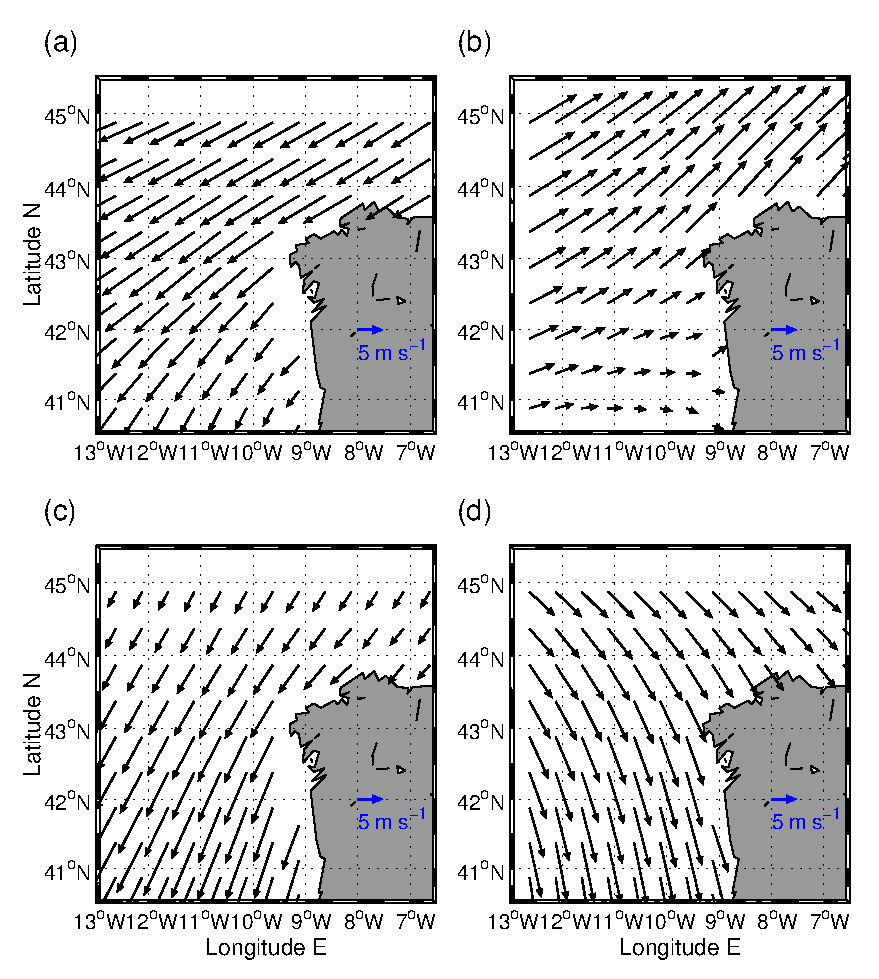
\includegraphics[height=12cm,keepaspectratio=true]{patrones99-00}
\caption{Typical reconstructed wind patterns found in 1999-2000
showing combination of unit vectors for mode 1 and 2 directed, a)
30$^\circ$ and 30$^\circ$, b) 180$^\circ$ and 180$^\circ$, c)
0$^\circ$ and 150$^\circ$ and d) 300$^\circ$ and 150$^\circ$}
\label{fig:windsreconfig}
\end{figure}

Combining the mean field with the first two modes for the
preferred orientations ({Fig~\ref{fig:windsroseeof2}}) produces
winds fields that typify the entire 2 year record.
Figure~\ref{fig:windsroseeof2}a represents a combination of unit
amplitude vectors directed at 30\deg for mode 1 and 2 (but is
representative of a wider range of orientations $\pm$10\deg). This
wind field, dominant during March (shaded window in
Fig~\ref{fig:windsampseasonal}), shows intensified southwestward
winds parallel to the coast of Finisterre, slightly onshore on the
north coast and weaker and slightly offshore south of the Cape.
This pattern favours upwelling along the north coast between Cape
Finisterre and Estaca de Bares, and especially off Finisterre and
will be referred to here as the PUNC (Predominant Upwelling on
North Coast).

Figure~\ref{fig:windsroseeof2}b is a combination of unit amplitude
vectors directed towards 180\deg for both modes and shows a
typical pattern of downwelling winds. This situation with
northeastward winds stronger north of Finisterre, is found in
December and February. Varying the orientation of mode 2 produces
different downwelling intensifications north and south of
Finisterre. They will generically be referred to as DOWN
(Downwelling of West and North coast).

Figures.~\ref{fig:windsroseeof2}c and \ref{fig:windsroseeof2}d
correspond to orientations 0\deg (300\deg) and 150\deg (300\deg)
for mode 1 (mode 2) respectively and typify the dominant upwelling
patterns for summer 2000. Both wind fields are more intense along
the west coast and favour upwelling along the west coast over the
Finisterre and northern coasts (PUWC - Predominant Upwelling on
West Coast).

\subsection{The winter season of 2000-2001}
Unlike the winter wind regime of 1999-2000, which in many
respects, was similar to the summers 1999 and 2000,  the winter of
2000-2001 was more ``typical''. The median for November to April
(Fig~\ref{fig:windsmedian}d) showed a spatially coherent wind
field of $~5ms^{-1}$ with an E-SE direction near coast south of
43\deg N rotating to a E-NE orientation further north. The CEOF
analysis (20 Oct 2000-10 May 2001) yielded two modes (80\% and
10\% of the total variance respectively) similar to the ones
presented in the seasonal analysis of
Fig~\ref{fig:windseofseasonal}. Mode 1 represents a stronger wind
field ($\sim 9ms^1$) directed more parallel to the coast than that
depicted in Fig~\ref{fig:windseofseasonal}a, while mode 2 is
directed more in the offshore direction when compared to
Fig~\ref{fig:windseofseasonal}b. The mode 2 wind intensity is
similar in both analyses; however, the channel of maximum curl is
orientated more perpendicular to the west coast in winter 2000-1
so that the winter modes are more perpendicular to each other.
\begin{figure}
\centering
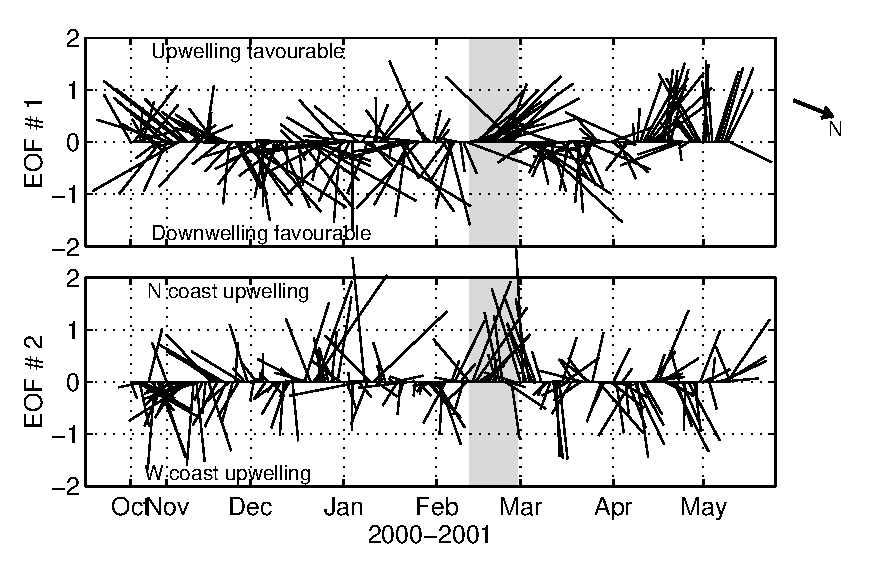
\includegraphics[height=8cm]{winter01_amplitude_new}
\caption{Amplitude time series for the winter 2001 analysis (20
Oct 2000-10 May 2001). The shaded intervals are referred to in the
text. The arrow on the left points at the geographical North for
the largely coherent wind field of Mode 1.}
\label{fig:winter_01_amp}
\end{figure}

The amplitude series ({Fig~\ref{fig:winter_01_amp}}) show that
sustained if variable DOWN wind fields were dominant, particularly
from late November until early April. From 12-28 February a PUNC
wind field,like March 2000 (Fig~\ref{fig:windsroseeof2}a)
occurred. Mode 2 contributes less overall to the wind field than
in the seasonal analysis with relatively few strong events.
Upwelling winds were more directionally consistent than
downwelling winds. The former can be grouped in two preferred
orientations: 310-340\deg and 0-40\deg, similar to
Fig~\ref{fig:windsroseeof2}d and c; downwelling winds fall into
two wider ranges: 270-280\deg  and 150-210\deg, westerlies and
southwesterlies similar to Fig~\ref{fig:windsmedian}d. Downwelling
patterns persisted for $<$6 days, while upwelling wind periods of
$<$14 days occurred in February and April to May.

The narrow, warm tongue indicative of poleward flow first appeared
over the slope in weekly SST average images in early December
after a week of downwelling favourable winds. Short upwelling
events like 11-15 January temporarily detached the poleward
current from the shelf but did not disrupt its SST signal.
Subsequent downwelling winds intensified the SST poleward flow
signal, which returned to its original position along the slope.
However the tongue disappeared from the north coast following 5
days of PUNC winds up to 12\vel. The SST signal of the flow was
not re-established until 11 March
(Fig~\ref{fig:windssstsummary}f), 10 days after the return to DOWN
winds. Winds changed to PUWC on the 6 April and remained
predominantly so until the end of the record on 10 May. The
upwelling response in this season appears slow. Although first
signs of weakening poleward flow occurred during 8-14 April, when
the SST differences between the warm tongue and oceanic waters
reduced, west coast upwelling did not appear until 29 April-5 May
after 14 days of continuous upwelling winds.


\section{PUNC wind pattern effects on upwelling}
\begin{figure}
\centering \noindent \subfigure[ Wind field 21 July]
{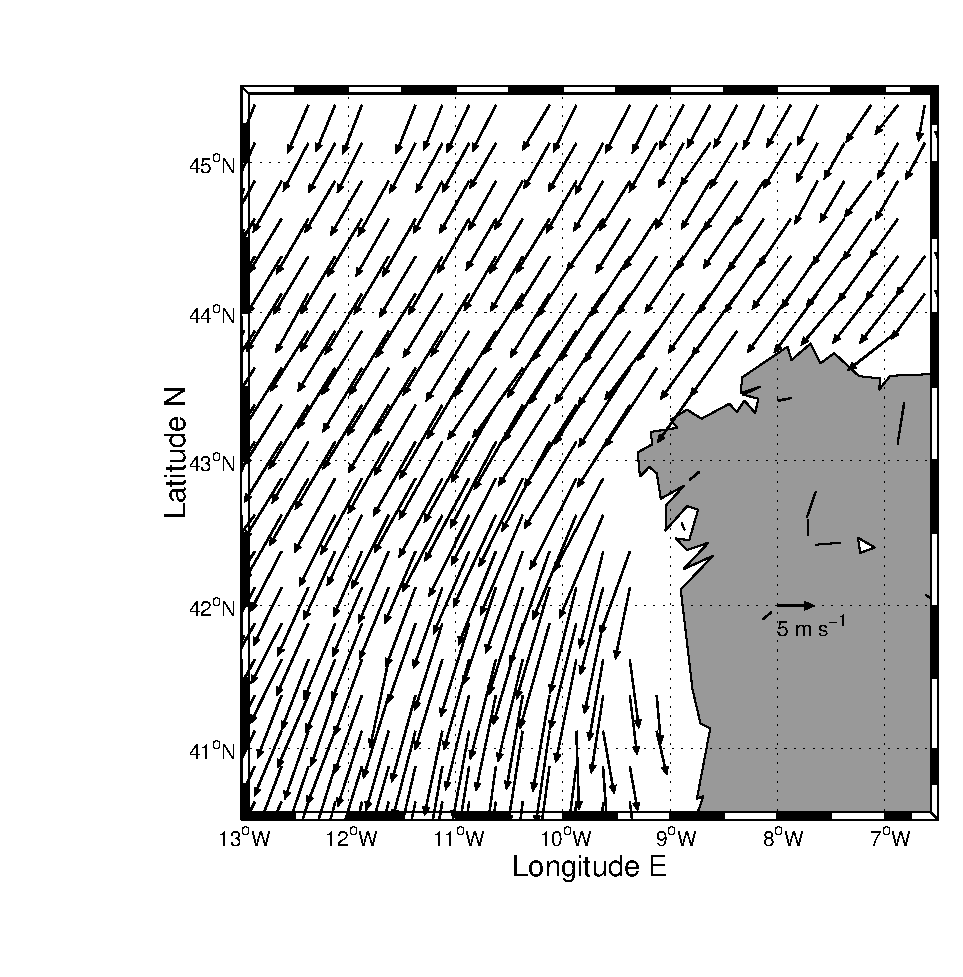
\includegraphics[totalheight=6.75cm]{21jul99winds}}
\subfigure[SST 21 July] {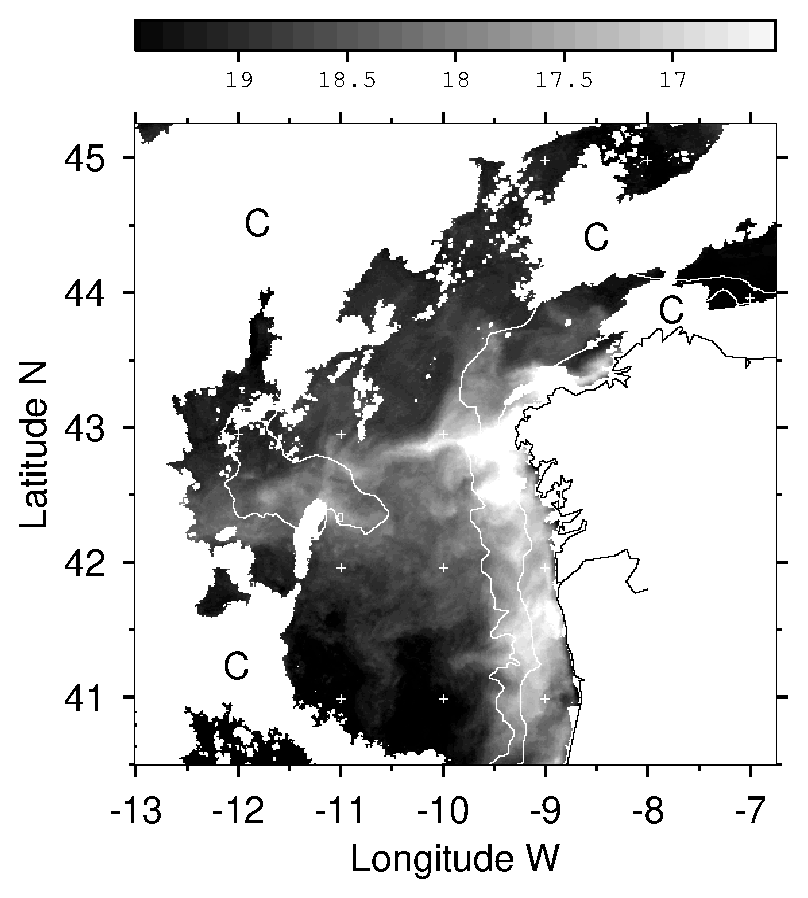
\includegraphics[totalheight=6.65cm
]{21jul991553gasstp}} \subfigure[Wind field 23 July]
{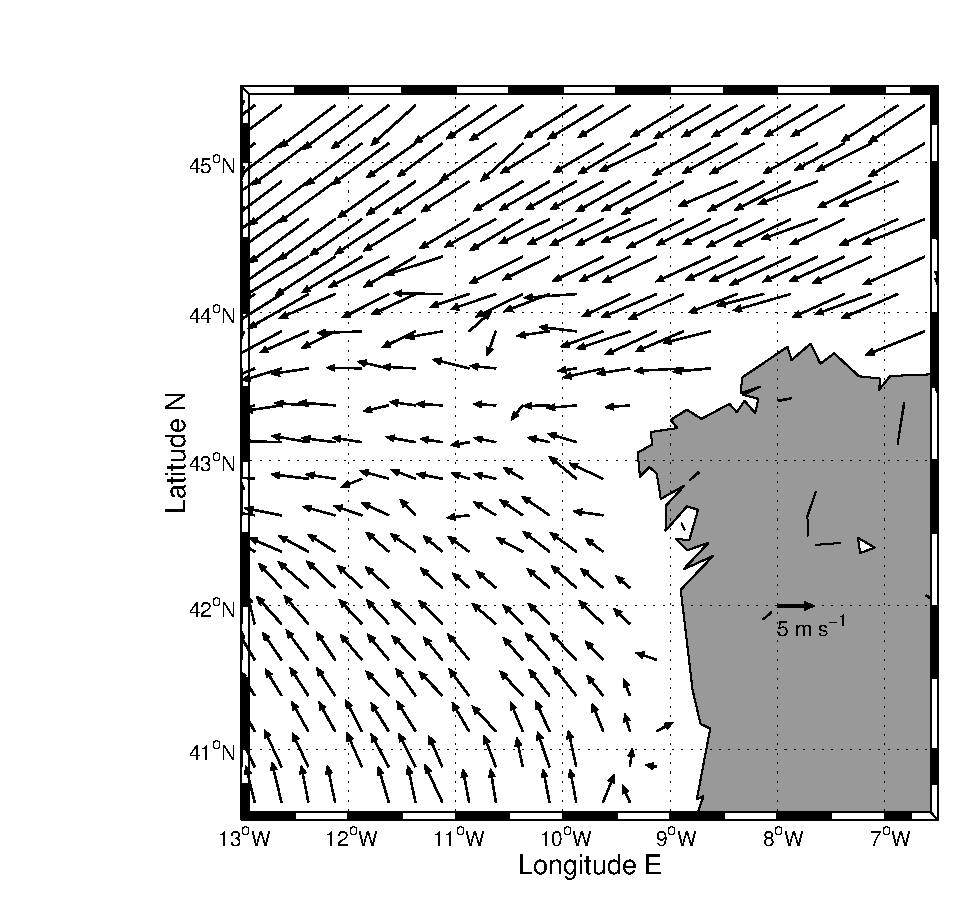
\includegraphics[totalheight=6.75cm]{24jul99winds}}
\subfigure[SST 23 July]
{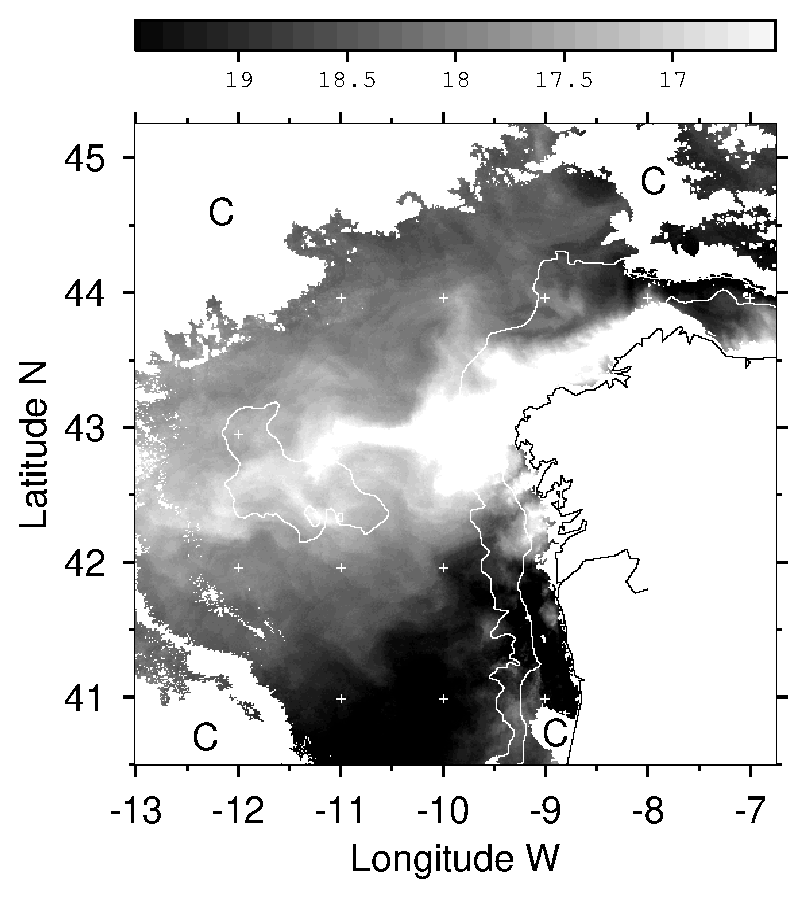
\includegraphics[totalheight=6.65cm]{23jul991530gasstp}}
\caption{ Wind fields and SST images from 21 and 23 July
1999.}\label{fig:windssst2123}
\end{figure}
Spatial variability of coastal upwelling can be explained largely
by the dominant wind patterns of Fig~\ref{fig:windsreconfig}.
Winds on the 21 July 1999 (Fig~\ref{fig:windssst2123}a) were PUWC
upwelling favorable similar to Fig~\ref{fig:windsreconfig}c. Winds
of speeds up to 10\vel\, parallel to shore forced strong upwelling
both at Finisterre and the west coast. The SST image for the 21
July (Fig~\ref{fig:windssst2123}b) shows minimum temperatures
around Finisterre and a clearly identifiable Finisterre filament.
West coast upwelling extended south to 41\deg N and offshore to
the 1000m isobath. Weak north coast upwelling persisted despite
onshore winds north of the Cape. However the wind rotated
clockwise through a PUNC pattern to that of 23 July
(Fig~\ref{fig:windssst2123}c), dominated by mode 2 as in
Fig~\ref{fig:windseofseasonal}b. This enhanced upwelling in the
north coast, strengthened the Finisterre filament, but was
downwelling favorable on the west coast
(Fig~\ref{fig:windssst2123}d). Although this particular pattern
with northward winds south of Finisterre is infrequent, strong
development of the Finisterre filament to the exclusion of those
further south in e.g. 1995 and 1996, suggests similar PUNC wind
fields can predominate over part of the upwelling season.

\subsection{Coastal Wind Buoy measurements}
\begin{figure}
\centering \subfigure[]{
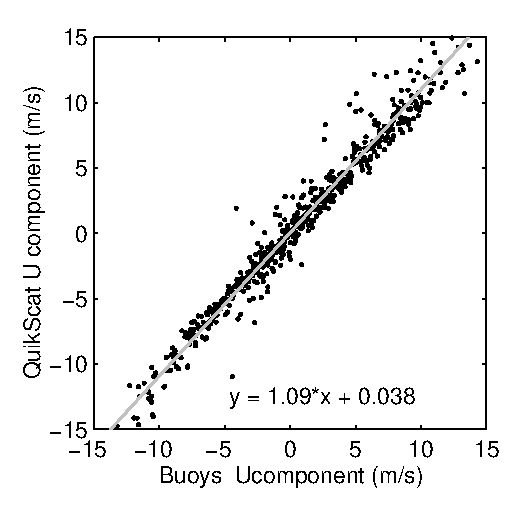
\includegraphics[height=6cm]{buoycalU}}
\subfigure[]{
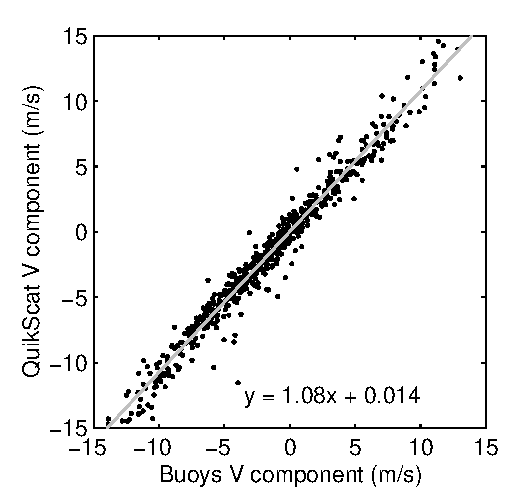
\includegraphics[height=6cm]{buoycalV}}
\caption{Comparison between QuikScat and coastal Buoys during the
period of study for (a) U and (b) V wind components. The resulting
linear fit is included.}\label{fig:windsbuoycal}
\end{figure}

The DWN buoy observations allow extension of the analysis to the
period when the Finisterre filament was starting to develop but
before QuiKSCAT data are available. Both data are compared in
Fig~\ref{fig:windsbuoycal} for the common periods and are
simultaneous in time to the closest hour. The data agreed well
with correlations $r^2=0.96,0.97$ (their coefficients significant
at 99\% level of confidence, F=24893, 31423, df=1023, p$<$0.001)
for the U and V components respectively. Linear regression model
for both components were,
\begin{eqnarray}
  QU = 1.09\,(\pm 0.00044)\times BU + 0.038\,(\pm 0.0024),\label{eq:BcorrU} \\
  QV = 1.08\,(\pm 0.00038)\times BV + 0.014 \,(\pm 0.0021),\label{eq:BcorrV}
\end{eqnarray}
in which Q and B stand for QuikScat and Buoys data for each the U
and V components. The QuikScat data is consistently larger than
the Buoys data by less than 10\% which could be explained by the
more offshore position of the QuikScat grid locations.
\begin{figure}
\centering
\includegraphics[height=12cm,keepaspectratio=true]{eof_complex_allphd}
\caption{Mean field (a), the variance (b), and Eofs \#1 (c) and
\#2 (d) of the wind data available during the upwelling season of
1999, 1-May to 15-August for the offshore
buoys.}\label{fig:windsmeanvarbuoys}
\end{figure}

The daily median of the hourly winds were used to calculate the
CEOFs for the period 1-May-1999/15-August-1999
(Fig~\ref{fig:windsmeanvarbuoys}). No data were recorded
afterwards due to instrumental failure. The first two modes
explained 87\% of the total variance of the 107 days record and
are statistically distinct (Fig~\ref{fig:windsmeanvarbuoys}b). The
mean winds (Fig~\ref{fig:windsmeanvarbuoys}a) are very small
reflecting the averaging over non-upwelling and upwelling periods.
Mode 1 (Fig~\ref{fig:windsmeanvarbuoys}c) represents stronger
north coast upwelling. Mode 2 (Fig~\ref{fig:windsmeanvarbuoys}d)
represents opposing winds at the S  and N buoy and null near
Finisterre, strongly similar to the corresponding QuikScat mode.
This similarity is remarkable considering the difference in record
length and timing. When both modes are positive the wind becomes
less upwelling favorable off the north coast (N buoy), and more so
off the west coast (S buoy). When only mode 2 is negative the wind
is more upwelling favorable along the north coast and less so off
the west coast.
\begin{figure}[t]
\centering
\includegraphics[height=8cm,keepaspectratio=true]{amplitude_complex_all}
\caption{Amplitude Time series of the wind analysis in 1999. The
shaded intervals are referred to in the text. The arrow on the
left points at the geographical North for the largely coherent
wind field of Mode 1.}\label{fig:windsampbuoys}
\end{figure}

The amplitude time series ({Fig~\ref{fig:windsampbuoys}}) show
periods of alternating upwelling and downwelling favorable
conditions. The first consistent upwelling favorable period was
 7 to 23-June (Fig~\ref{fig:windsampbuoys}a)when the first signs of
upwelling were seen in SST images. The period was structured into
two pulses; each started with northerly winds that gradually
strengthened and rotated to north-easterly, then weakened and
rotated to easterly winds. During this development, more during
the second pulse, mode 2 became more negative, favoring north
coast upwelling and west coast downwelling. The SST images for the
same period show the development of strong upwelling in the north
coast, weaker upwelling along the west coast, and the progressive
advection of the cold upwelled coastal waters directly offshore at
Cape Finisterre. From 24 June till 6 July, downwelling winds
weakened the Finisterre filament, then renewed upwelling winds
strengthened it again. This time, mode 2 was strongly negative
producing the same wind pattern identified for 22-23 July in the
QuikScat observations (Fig.~\ref{fig:windssst2123}c).

\subsection{Coastal Current Buoy measurements}
\begin{figure}
\centering
\includegraphics[height=12cm,keepaspectratio=true]{eof_complex_all_currphd}
\caption{Mean field (a), the variance (b), and Eofs \#1 (c) and
\#2 (d) of the current data available during the upwelling season
of 1999, 1-May to 15-August for the offshore
buoys.}\label{fig:windsmeanvarbuoyscurr}
\end{figure}

The CEOFs for the buoy current data (1 May-15 August 1999) were
calculated as for the wind data. The mean current
{Fig~\ref{fig:windsmeanvarbuoyscurr}}a is significantly different
from zero (F, 8.3\velc ) only off Finisterre where it is directed
westward i.e. alongshore equatorward and slightly offshore. Mode 1
(Fig~\ref{fig:windsmeanvarbuoyscurr}c) accounted for 75\% of the
variance and shows stronger variability off Finisterre and the
north coast (F and N, $\sim$8.5\velc ) than off the west coast (S,
$\sim$3\velc ). Mode 2 (Fig~\ref{fig:windsmeanvarbuoyscurr}d)
accounted for 15\% of the variance and represents diverging
vectors at the northern buoys (N and F) and negligible
contribution from site S. This contrasts with wind mode 2, which
showed opposed north and west coast winds. For both modes, the
axes of maximum variability are directed such that flow is in the
equatorward and offshore or poleward and onshore sense, as
expected for the local wind driven regime.

\begin{figure}[t]
\centering
\includegraphics[height=8cm,keepaspectratio=true]{amplitude_complex_all_curr}
\caption{Amplitude Time series of the current analysis in 1999.
The arrow on the left points at the geographical North for the
largely coherent field of Mode 1.}\label{fig:windsampbuoyscurr}
\end{figure}
The amplitude time series of {Fig~\ref{fig:windsampbuoyscurr}}
show the expected poleward flow for the downwelling regime during
the first half of May. The change to the upwelling regime is seen
in mode 1 on the 9-June, two days after the onset of the upwelling
winds. Thereafter, the circulation corresponds mostly to upwelling
but wind reversals produced short lived current reversals (e.g.
end of June) or weakening of the upwelling (e.g. end of July).
Peak offshore velocities at buoy F coincide with wind peaks, which
favour the Finisterre filament, reaching values of 22\velc . In
the first half of May, the mode 2 contribution enhanced the
poleward tendency at F but weakened it at N, partly compensating
for the more equatorward mean at F. From June on, it opposed the
equatorward flow at F and enhanced it at N, again tending to
reduce the difference in actual flow at both.

\subsection{Comparison with other years}
\subcapnoonelinetrue \subfiguretopcapfalse
\begin{figure}[t]
\centering \subfigure[June 18-24]
{\includegraphics[height=6cm]{ga950618}}\quad \subfigure[August
06-12] {\includegraphics[height=6cm]{ga950806}}\quad \caption{SST
weekly averaged images from 1995. Arrows labelled F mark known
locations for filaments. Arrows labelled N mark the north coast
site with largest upwelling differences.}\label{fig:windssst95}
\end{figure}

The Finisterre filament followed similar development in 1995 and
1999. Coastal upwelling first appeared in SST imagery at the end
of May along both coasts but a week later upwelling was mainly
north of Finisterre. By the 11 June 1995 a filament extended 125km
from the cape and upwelling on the west coast had disappeared
({Fig~\ref{fig:windssst95}}a). This situation persisted through
July but By August, north coast upwelling had weakened. Lowest
temperatures were located on the west coast, where upwelling
extended to the 1000m isobath. After the 6 August frontal
instabilities started to develop ({Fig~\ref{fig:windssst95}}b) at
43.25\deg N (off Finisterre) and at 42.25\deg N and 41.25\deg N,
other well known locations for filaments
\nocite{Haynes93}[\markcite{{\it Haynes et al., }1993}]. They
continued to grow until 27 August when upwelling was
re-established north of Finisterre. The Finisterre filament
continued to grow as the west coast upwelling weakened. After 17
September, the situation of August was repeated, i.e. the
Finisterre filament retreated, upwelling weakened north of the
Cape  while it intensified further south, and the instabilities
developed again.  This evolution can be explained by alternation
of the typical PUNC and PUWC wind patterns of
Fig~\ref{fig:windsreconfig}a and d, favoring upwelling on one or
other of the coasts.

\noindent \subfiguretopcaptrue
\begin{figure}[t]
\centering \subfigure[] {\includegraphics[height=6cm]{mar00}}\quad
\subfigure[] {\includegraphics[height=6cm]{jun95}}\quad
\subfigure[] {\includegraphics[height=6cm]{jul95}}
\caption{Monthly averages of Sea Level Pressure for March 2000,
and June and July 1995}\label{fig:windsslp}
\end{figure}

Though no \emph{in situ} wind observations are available for 1995
this interpretation is supported by Sea Level Pressure (SLP) data
from the National Centers for Environmental Prediction (NCEP)
Reanalysis project at the Climatic Diagnostics Center web site
[{\it http://www.cdc.noaa.gov/cdc/reanalysis/}].  The SLP field in
June 1995 (Fig~\ref{fig:windsslpfig}a)  indicates winds parallel
to the north Iberian coast and offshore on the west coast, as in
the PUNC pattern of Fig.~\ref{fig:windsreconfig}a, with tight
packing of the isobars indicating strong winds at Finisterre.
During July 1995 the SLP field (Fig~\ref{fig:windsslpfig}b) shows
the Azores High well to the south (33\deg N, 40\deg W), producing
a PUWC wind pattern similar to Fig~\ref{fig:windsreconfig}c that
favored west coast upwelling and weakening of the Finisterre
filament, as was observed (Fig.~\ref{fig:windssst95}b).

\section{PUWC wind pattern effects on upwelling}
\label{nofinisterre}
\begin{figure}
\centering
\includegraphics[height=9cm,keepaspectratio=true]{summer99_00amplitude}
\caption{Amplitude Time series for the summers 1999 (19 Jul-30
Sep) and 2000 (1 May-31 Oct). The shaded intervals are referred to
in the text. The arrow on the left points at the geographical
North for the largely coherent wind field of Mode 1.}
\label{fig:windsamp9900}
\end{figure}

In some years, the Finisterre filament does not develop and west
coast upwelling with (e.g.~1998) or without (e.g.~2000) filament
development dominates. The CEOF mode 1 amplitude time series for
summers 1999 (19 Jul-30 Sep) and 2000 (1 May-31 Oct) accounted for
76\% and 72\% of the variance respectively. The mean fields were
similar in both summers (Fig~\ref{fig:windsmedian}a and c) to the
typical PUWC pattern (Fig~\ref{fig:windsreconfig}d) and in both
the first two modes (not shown) were like the overall modes
(Fig~\ref{fig:windseofseasonal}a and b). However, during summer
1999 few wind events lasted long enough to produce significant
west coast upwelling (shaded in Fig~\ref{fig:windsamp9900}a) and
filaments. During summer 2000, repeated short west coast upwelling
events of various intensities again alternated with shorter
downwelling periods. Even the two most persistent upwelling events
(6-19 July and 31 July-10 August) generated only short 80 km
filaments at 42.25\deg N and 41.25\deg N
(Fig~\ref{fig:windssstsummary}e) that weakened after each event.

In contrast, west coast upwelling and full filament formation
dominated during July 1998, when sustained upwelling favourable
winds occurred from June \citep{Smyth01}.  During June-August a
series of filaments formed, grew and merged near 41.25\deg N,
42\deg N and 43\deg N. During August both Finisterre and west
coast upwelling coexisted although the former did not develop a
filament and west coast upwelling persisted until September
\citep{Barton01}. {Fig~\ref{fig:windsamp9900}}a-b show the monthly
SLP field for July and SST image for 29 July, 1998. During July,
the mean field shows the well defined Azores high with strong
winds parallel to the west coast of Iberia producing the west
coast upwelling and development of the 42\deg N filament
(Fig~~\ref{fig:windsamp9900}b).
\begin{figure}[t]
\centering \subfigure[] {\includegraphics[height=6cm]{jul98}}
\subfigure[] {\includegraphics[height=6cm]{29jul981519gasstp}}
\caption{(a) Monthly average of Sea Level Pressure July 1998 and
(b) SST image of 29 July 1998.}\label{fig:windsslp98}
\end{figure}



%\subsubsection{Current measurements}
%Although no current meter data are available for winter 2001, data
%from 2000 can be used to determine the influence of the different
%wind conditions on the coastal flow at the three buoys.
%Fig~\ref{fig:tswinter} shows time series of Mode 1 magnitude and
%direction for the QuikScat data CEOF analysis and along-shelf
%component of flow at the three buoys between 16 February and 22
%June 2000. The Mode 1 data have been rotated so that 0\deg
%represents the North. A unit magnitude at 0\deg represents a wind
%field of $\sim$10\vel\, flowing southward. Note that the effect of
%the mean wind field is to increase equatorward component on the
%west coast but have relatively little effect on the north coast
%(Fig~\ref{fig:windsmeanvar}a). The mode 2 variation is generally
%less significant except as pointed out below. Stronger currents
%were measured at the Bares buoy (N) and the variance increased
%northward along-shelf. Maximum poleward velocities at N reached
%values of 20\velc, decreasing to 15\velc\, at F and 9\velc\, at S.
%The last two showed poleward flow during most of the record up
%until 14 May while buoy N recorded more equatorward flow events.
%The first part of the record is characterized by slow winds and
%poleward flow at the three buoys around 21-27 February but later
%changing to equatorward flow around 4 March with the onset of
%winds similar to Fig~\ref{fig:windsroseeof2}a but aligned more in
%the East-West direction. Although winds remained unchanged for 10
%days the flow started to turn poleward at S and F while flow at N
%became less equatorward. This poleward tendency could be
%associated with the mode 2 positive wind curl off and south of
%Cape Finisterre (Fig~\ref{fig:windseofseasonal}b) forcing poleward
%flow along the west coast and towards buoy N where it was opposed
%by the relatively stronger equatorward mode 1 wind stress on the
%north coast. A further increase in wind speed to 13\vel\, together
%with a change towards more northerly wind direction weakened the
%poleward flow in all three sites. Further poleward flow peaks
%coincided with westerly or weak winds which affected the northern
%buoys most, as on 25 March and 1 April. After 9 April moderate to
%strong winds with a range in directions 200\deg-270\deg forced the
%largest poleward flow response of the record affecting all three
%buoys. The maximum flow was measured on 19 April with westerly
%winds of $\sim$13\vel\, but weakened after 25 April when winds
%decreased and became northerly. However, flow stayed poleward and
%a secondary maximum was reached on 9 May with a further decrease
%in wind speed and a change in orientation to east-northeasterly
%winds. The poleward current flowed against winds too weak to
%balance the northward pressure gradient. Currents then decreased
%and turned equatorward in coincidence with northerly winds. Around
%day 28 May, westerly winds resulted in near zero flow on the west
%coast and strong poleward (i.e. eastward) flow at N. For the rest
%of the series currents were weakly equatorward at S, slightly more
%so at F and almost zero at N. This was related to variable weak
%winds from the NE or NW. In general, variability was greater on
%the north coast, but on the west coast and off Finisterre up to
%mid May, currents were predominantly poleward, then mainly
%equatorward. Fluctuations were largely but not entirely related to
%variations of the first wind mode with lesser influence of mode 2.
%\begin{figure}
%\includegraphics[height=10cm]{poleward}
%\caption{Time series of Measured (a) wind amplitude (b) direction
%series from the seasonal CEOF mode 1, and alongshelf components of
%(c) currents at Silleiro, (d) Villano-Sisargas and (e) Bares buoys
%for the period 16 Feb-22 Jun 2000.} \label{fig:tswinter}
%\end{figure}
%



\section{Discussion}
The period under study, July 1999 through to May 2001, showed no
clear seasonal wind signal with upwelling and downwelling winds
distributed year-around. Similar results were obtained by
\citet{Nogueira98}, who found that only 20\% the variability in
daily Ekman transport off Cape Finisterre over 9 years was
associated with the seasonal cycle, while 70\% concentrated at
frequencies $<$30 days.onal cycle, while 70\% was concentrated at
frequencies $<$30 days. \citet{Nogueira97} showed from harmonic
analysis that the average upwelling event length was $T=15\pm 5$
days, close to our estimate of $14\pm 2$ days. Comparing our data
with those of \citet{Kosro91} off California, we observe that
although cycles of upwelling-winds/relaxation take place in both
regions, Galicia is more variable in wind speed, direction and
persistence. Much of the summer variability relates to
anticyclones moving northeastward over the bay of Biscay.

Differing patterns of upwelling favourable wind fields force
different responses in the system favoring either north or west
coast upwelling (PUNC and PUWC, respectively). Summer 1999
experienced winds favorable to north coast upwelling and Cape
Finisterre filament development while summer 2000 was more
typified by west coast upwelling. Both years experienced highly
variable winds that did not persist long enough for upwelling
filaments to develop on the west coast. The strongest development
of west coast filaments in recent years occurred in 1998, when
west coast upwelling-favorable winds lasted from June to early
August with few interruptions. These sustained upwelling favorable
winds maintained a sharp upwelling front that allowed the
development and growth of the west coast instabilities into
upwelling filaments.

Much has been hypothesized about the generation of upwelling
filaments.  \citet{Roed99} and \citet{Haynes93} reported a clear
link between bottom topography and filament formation in the
Galician region on the basis of models and observations,
respectively. However, in the case presented here, the Cape
Finisterre filament is clearly dependent on particular wind
conditions for its development. The mere presence of upwelling at
Finisterre is not sufficient. Although small scale instabilities
sometimes develop off the Cape (see Figs~\ref{fig:windssst2123}b,d
and \ref{fig:windssst95}a), it requires a well developed north
coast upwelling for them to grow into a full sized filament. At
these times the wind field is like that of
Fig~\ref{fig:windsreconfig}a and the filament extends offshore
along the line of maximum wind curl identified in mode 2 in
Fig~\ref{fig:windseofseasonal}.
\begin{figure}
\centering
\includegraphics[height=8cm]{ekman_pum_1999723}%ekman_pum_1999723}
\caption{Vertical Ekman pumping velocities on 22 July 1999 in
m/day, positive upwards.} \label{fig:ekman}
\end{figure}

This maximum wind curl produces upwelling velocities given by
\(w=k\cdot(\nabla \times \frac{\tau}{f\rho} )\), where $k,\tau,f$
and $\rho$ are vertical unit vector, wind stress, Coriolis
parameter and density of water. This Ekman pumping is caused
solely by the divergent Ekman fluxes in the presence of spatially
variable wind and is unrelated to the coastal upwelling.  An
example is shown in Fig~\ref{fig:ekman} for measured winds on 22
July 1999 corresponding to a wind field similar to
Fig~\ref{fig:windsreconfig}a. Positive Ekman pumping velocities
indicative of upwelling can be seen south of the maximum wind curl
northern limit in Fig~\ref{fig:windseofseasonal}b and towards the
west coast. Maximum vertical velocities coincided with the axis of
maximum curl and decreased from 6\veld near Cape Finisterre to
1\veld farthest offshore. Calculations on a similar day in March
2000 yielded a similar pattern except vertical velocities were
smaller by a factor of 2 and decreased rapidly on the west coast.
The strong winds in June 1995 (Figs~\ref{fig:windsslp}a and b)
were again like the 1999 case. We conclude summer occurrences of
this wind pattern lead to upwelling velocities of 5-6\veld off
Cape Finisterre. These are smaller than the ones (up to 20\veld)
reported by \nocite{munchow00}\markcite{{\it M\"{u}nchow }[2000]}
off Point Conception, California. His finer sampling covered a
much smaller area which defined a maxima wind curl ridge 80km long
and 10km wide. In our case, the ridge extends 320km in length and
90km in width and vertical velocities are likely to reach higher
values nearer to the shore at Cape Finisterre.
\begin{figure}
\centering
\includegraphics[height=8cm]{wind_july9977march00320}
\caption{Example of measured winds from the offshore buoys on 7
July 1999 (black) and 20 March 2000 (red).} \label{fig:rev}
\end{figure}

\citet{Munchow00} reported flow separation in the wind field at
Point Conception in the presence of upwelling. He argued that the
lower sea surface temperatures enhanced the vertical stability of
the marine layer, which is capped by a temperature inversion.
Coastal upwelling can modify air temperatures by as much as
1-5\deg C over timescales of 12-24 hours \citep{Samelson02}. As in
\citet{Enriquez95}, the marine layer flow becomes supercritical
and separates from the coast causing the wind curl and Ekman
pumping velocities. We see some evidence of wind flow separation
in the lee of Cape Finisterre during the summer upwelling regime.
For example the buoy wind data for 7 July 1999 (Fig~\ref{fig:rev})
show measured north coast and Finisterre winds flowing nearly
opposite to west coast winds, suggestive of strong flow separation
at the cape. Similar north coast winds were common throughout
March 2000 and after 14 June 1999, but flow separation only
occurred in the presence of cold upwelled water around Cape
Finisterre during the 1999 examples. Hence, there are some
evidences that the PUNC strengthen both near the coast and after
the start of the coastal upwelling generating larger wind curl and
associated Ekman pumping velocities increasing shorewards. The
positive wind curl would cause a poleward alongshore pressure
gradient as indicated by model studies of \citet{Wang97}. However,
finer scale wind observations near Finisterre and atmospheric
observations would be needed to reach a definitive conclusion.

The existence of recurring wind curl west of Cape Finisterre will
influence the vertical water structure to cause doming of the
isopycnals. \citet{Munchow00} showed that a similar wind curl
influenced the vertical water structure to cause doming of the
isopycnals.  A similar local effect on the shelf circulation may
be expected around Cape Finisterre. The systematically weaker
southward velocities observed at the west coast buoy (S) compared
to the Finisterre buoy (F) are consistent with such a cyclonic
tendency but we presently have no hydrographic evidence to verify
it. Capes also have a significant impact on the alongshore
variability of the upwelling flow field
\citep{Crepon84,Dale01,Rosenfeld94}, producing nonlinear effects
accompanying the acceleration of the flow around the capes, and a
cyclonic tendency downstream. Doming could help explain the
persistence of the Finisterre filament following cessation of
favourable wind patterns, but again, observational evidence of the
detailed hydrographic and current structure near the cape is
lacking.


Winter winds in general showed larger variability than summer
winds during both a ``typical'' (2000-2001) and ''atypical''
(1999-2000) seasonal year. Downwelling wind patterns emerged from
CEOF analysis during both the 1999-2000 and winter 2001 analyses.
E,NE and N winds were predominant during both winters reaching
speeds in the range 15-20 \vel, higher than the 10-15 \vel range
of summer winds. However their persistence was far less (4-6 days)
than during summer ($\sim$12 days). Both winters saw the PUNC wind
field predominate during sustained periods in March and February
respectively. Its effect on the SST field was the disappearance on
the north coast, but not the west coast, of the warm temperature
anomaly indicative of poleward flow only.

It is difficult to define transitional regimes, non-upwelling to
upwelling and vice versa in terms of the wind forcing because of
the absence of any clear seasonal cycle.  Extension of the
analyses to a longer period will provide better information, but
it appears that as long as the meridional sea surface temperature
gradient is present, (nearly until July) upwelling winds do not
fully set up upwelling; even sustained winds provoking upwelling
early in the season do not develop filaments, e.g. April-May 2001.

\section{Conclusions}
Investigation of the QuikSCAT and in situ wind fields in the
Galician upwelling region around Cape Finisterre has shown:
\begin{itemize}
  \item    The wind field is far from homogeneous in the region so that
wind observations at a single point, coastal or offshore, will not
necessarily be representative of coastal conditions over any
significant distance.

  \item   The wind field's long-term mean summer and winter patterns are
not necessarily representative of particular years when, as we
have seen, summer-like patterns may dominate in winter also.

  \item   Similar Wind Modes were obtained in all CEOF analysis, of both
satellite derived and \emph{in situ} buoy measurements, and of
different length and seasonal period.

  \item   Summer time wind fields have a small number of dominant
patterns, discernible in complex empirical orthogonal analysis,
that are responsible for the typical distributions of upwelling in
and off the Galician coast.

  \item   One pattern produces north coast, but no west coast,
upwelling. In years when this pattern dominates, the Cape
Finisterre filament is strong but no others develop. The filament
is partly supplied by cold water from the north coast but also,
importantly, by local open ocean upwelling produced by the wind
stress curl, which extends in a maximum SW from the cape.

  \item   Another pattern produces west coast upwelling, but no
north coast upwelling.  When this pattern persists, west coast
filaments develop at favored locations other than Finisterre and
may extend up to 200km offshore.

  \item   These patterns may alternate producing brief episodes or north
or west coast upwelling with little filament development, or a
combined pattern may occur that produces weak upwelling on both
coasts with a localized maximum at Finisterre, where the wind lies
parallel to the coast.

  \item   Winter time wind patterns show strong similarities to those of
summer, symptomatic of frequent short occurrences of winter
upwelling during our study years.

  \item   The onset of the winter poleward flow regime as indicated by
presence of the warm water anomaly along the continental slope is
delayed after the cessation of summer upwelling winds.  Likewise
the spring onset of upwelling lags significantly the commencement
of favorable winds, though subsequent upwelling events respond
rapidly to wind changes.

  \item   North coast currents were more variable in all records
  and showed the largest velocities.
\end{itemize}



\graphicspath{{d:/PhD/chapter2/graphics/}}
%
\chapter{Spring transition}\label{ch:spring}
\section{Introduction}
The spring transition is here taken to be the period during which
the winter regime of predominant downwelling and poleward flow
over the slope is replaced by a regime of sustained coastal
upwelling. In Chapter~\ref{ch:winds} it was shown that the
transitions between regimes are largely determined by the seasonal
cycle in the meridional density gradient inferred from SST. The
first stages of this transition are characterised by large
variability in both circulation and property distribution on the
shelf and offshore. In the absence of the steady sea level
gradient and stratification, the response of the Galician system
to upwelling favourable wind is stronger than in summer
\citet{Castro00}. During the transition, there could be short
periods during which poleward flow offshore and upwelling
nearshore coexist.

The spring transition between downwelling and upwelling regimes
can be found in all major eastern upwelling systems with a
seasonal cycle. The transition is fast in the California system
\citep{Huyer83} with a time scale of few days. Equally the
response of the Galician system to upwelling winds during the
spring transition has been estimated to be fast. In other regions
like the Canary Current upwelling system, no transition is
reported though there is a lack of systematic year round
observations.

The Rias Bajas have recently started to be regarded as an
intrinsic component of the ``shelf system'' that respond to
similar forcings, i.e. large scale and local winds can drive their
circulation pattern, more so during summer when freshwater input
is at its minimum. The downwelling winds and the presence of the
poleward flow over the shelf prevents the ``outwelling'' or water
discharge from the Rias Bajas, detaining it at the inner shelf
stations \citep{Castro97} and even forcing shelfwater into the
Rias Bajas at times \citep[e.g.][]{Prego01,Sordo01}. During
upwelling winds, the Rias Bajas behave like an extension of the
shelf \citep{Doval98} and upwelling takes place inside the Rias
\citep{Alvarez-Salgado00} enhancing the flushing of the Rias.

In the next sections data from a cruise in June 1997 coincident
with the spring transition are analysed. The cruise is put into a
broader temporal context by using SST images before and after the
cruise. The sampling strategy is presented first, followed by the
data description and analysis techniques.  Horizontal and vertical
distribution of properties and velocity vectors are described next
and particular attention will be placed on the interaction of the
outflow from the Rias and the offshore circulation. The Chapter
finishes with the discussion and main conclusions.

\section{Cruise description}
The RRS Charles Darwin Cruise 105 took place in the Galician CTZ
from 29 May to 20 June 1997 as part of the OMEX II-II project. The
cruise was divided into two legs: leg A ran from 29 May to 8 June
while leg B ran from 10 to 20 June. The main objectives of the
cruise were:

\begin{itemize}
  \item  to make a detailed swath bathymetry of the slope topography of the
  region during leg A.
  \item  to deploy a
bottom-mounted acoustic Doppler current profiler at 156m depth and
a mooring of four current meter in 686m, both near 42\deg 40'N,
  \item to sample a grid of CTD stations typically 10km apart on
  cross slope sections ranging from 43\deg N to 41\deg 25' every 10' of latitude
  and covering depths from 100m on the shelf to 3000m offshore,
  \item to record underway ADCP, temperature, salinity,
  fluorescence, transmittance and irradiance.
\end{itemize}
The sampling of the slope bottom topography was carried out during
leg A and only underway Temperature and Salinity were recorded for
that period. The CTD grid sampling took place during leg B. The
grid stations were roughly separated 10 by 18 km, smaller than the
local internal Rossby radius of 20-30km which provided enough
detail to resolve mesoscale structures. However, the 10 days it
took to complete the survey compromised its synopticity. Besides
the standard CTD measurements of temperature, salinity and
pressure, the instrument was also equipped with a fluorescence
sensor.

Downwelling favourable wind conditions were typical for the first
4 days of Leg B with increasing northerly winds thereafter until
the end of the cruise on 20 June. The moorings were deployed on
the first day (10 June) and the CTD grid started on the following
day. The 3 northernmost grid lines (Transects N,O and P,
Fig~\ref{fig:cd105stations}) were done first during downwelling
wind conditions, while the remainder of the grid was completed
northwards from the southern most deep station in the order V-Q
under upwelling conditions.
\section{Data and Methods}
\subsection{CTD}
A total of 82 CTD stations were sampled with a Neil Brown Systems
Mk IIIB CTD including a pressure sensor, a conductivity cell, a
platinum resistance thermometer and a Beckmann dissolved oxygen
sensor. The CTD unit was mounted vertically in the centre of a
protective cage approximately 1.5m square. A Chelsea Instruments
Aquatracka configured as a fluorometer was also attached to the
system.

A General Oceanics 12-bottle tone-fire rosette pylon was fitted to
the top of the CTD frame. 10-litre Niskin bottles were used
throughout the cruise.

On each cast, the CTD was lowered continuously at 0.5 to 1.0\vel\,
to about 20-30m from the sea floor. The data were logged by the
NERC Research Vessel Services (RVS) ABC data logging system.
Output channels from the deck unit were logged at 32 Hz by a
microprocessor interface (the Level A) which passed time-stamped
averaged cycles at 1 Hz to a Sun workstation (the Level C) via a
buffering system (the Level B).
\begin{figure} \centering
\includegraphics[width=7cm]{cd105stations}
\caption{Location of Coastal weather and CTD stations and Transect
names for CD105 cruise} \label{fig:cd105stations}
\end{figure}

The data were subsequently transferred to the British
Oceanographic Data Centre (BODC) where it was converted to
specific BODC data format. The data were separated into downcast
and upcast and edited for spikes or spurious data. The downcasts
were logged into the BODC system, calibrated and binned to 2dbar
prior to their release to the OMEX II community.

The temperature sensor was calibrated against on board
measurements from a digital reversing thermometer at depths
greater than 1000m. Agreement was found within the manufacturers
specifications and no correction was applied.

The salinity sensor was calibrated against 47 bottle samples
analysed on a Guildline Autosal bench salinometer and a constant
offset of 0.024psu ($\pm$0.005psu) was applied.

\subsection{Underway measurements}

The ship was fitted with a non-toxic pumped sea water supply with
water drawn from an inlet approximately 5m below the surface,
amidships on the starboard side. All ship's discharges were to
port to minimise risk of contamination. Water from the non-toxic
pump was fed into the thermosalinograph and the tank containing
the fluorometer and transmissometer.

Continuous data from the Falmouth Scientific Instruments
thermosalinograph were recorded every minute during both legs of
the cruise. During leg A only Temperature and Salinity were
recorded. In leg B,  chlorophyll data were measured by a Chelsea
Instruments Aquatracka fluorometer.

Where possible, data collected from underway sensors were
calibrated against CTD data and/or discrete samples from the
non-toxic supply or CTD rosette bottles. A constant offset of
-0.024\deg C (N=77,$\pm$0.0305\deg C) and -0.081psu
(N=85,$\pm$0.0109psu) were found for the temperature and salinity
sensors.

The data were also logged by the RVS ABC data logging system as
were the position data from GPS, primarily an Ashtech 3-D GPS
system.

\subsection{ADCP data collection and calibration}
\subsubsection{Instrumentation and acquisition}
A RDI Acoustic Doppler Profiler (ADCP) 150 kHz instrument was used
during the cruise.  The ADCP transducer transmitted sound pulses
every few seconds in four separate beams. Each beam was oriented
at a 30 degree angle from the ship's vertical axis. The transducer
was mounted roughly amidships at 5m below the water. The data
acquisition system consisted of an IBM-PC compatible computer
running the  RDI TRANSECT program. The navigational data and the
ADCP raw data were merged at the RVS ABC system level C. The
instrument was set up with a pulse length of 4m, a band width of
4m, a blanking interval of 4m, and an ensemble averaging of 5min.
The number of processed and recorded bins had been set to 100,
about twice the actual number of good bins. Because of the
additional processing time, the number of pings per ensemble was
greatly reduced and the quality of the final data set degraded.
The error velocity threshold for raw pings during acquisition was
1\vel\, and bins with less than 25\% of percentage good (PG) were
automatically flagged. No correction for pitch and roll were made;
errors associated with these are likely to be small
\citep{Kosro85}. The data were recorded continuously from 10 June
08:39 to 20 June 16:47.
\begin{figure}[tbh]
  \centering
  \begin{minipage}{7cm}
  \includegraphics[viewport=0 0 400 400,width=6.8cm,clip]{cd105adcptrack}
  \end{minipage}
  \begin{minipage}{7cm}
  \includegraphics[viewport=20 40 430 260,width=7.8cm,clip]{cd105lat}
  \includegraphics[viewport=17 40 430 260,width=7.8cm,clip]{cd105lon}
  \end{minipage}
  \caption{Cruise track and longitude and latitude displacement from ADCP during
   CD105 cruise}
  \label{fig:cd105track}
\end{figure}
The sampling track and the longitude and latitude time series
estimated from the edited GPS record are shown in
Fig~\ref{fig:cd105track}. The Percentage-good (PG) pings against
time and depth (bin number) during CD105 decreased towards the
bottom (Fig~\ref{fig:cd105pg}, darker colours indicate lower PG).
The black region of low PG can generally be related to
interference with the seafloor. The echo intensity from a hard
surface such as the bottom is much stronger than the echo from
scatterers in the water and for an ADCP with 30\deg beam angle,
the echo from the side lobes facing the bottom will return to the
ADCP at the same time as the echo from the main lobe at 85\% of
the distance to the bottom. This means that data from the last
15\% are usually contaminated and were therefore removed. The bulk
of the water column recorded values higher than 80\%, however the
first 1-2 bins appeared contaminated with values between 40-80\%
and were carefully inspected and dropped when necessary. The last
good record that had been used for plotting later in the chapter
was on 20 June 07:12 after which data degraded considerably due to
worsening of weather conditions.
\begin{figure}
  \centering
  \includegraphics[viewport=0 0 460 700,width=8.5cm,clip]{pgood160}
  \includegraphics[width=8.5cm]{pgood168}
  \caption{Percentage-good pings vs. time and bin number during CD105.}
  \label{fig:cd105pg}
\end{figure}

\subsubsection{ADCP data processing}
ADCP processing was done with the Common Oceanographic Data Access
System (CODAS), which includes MATLAB routines, developed at the
University of Hawaii by Eric Firing and Ramon Cabrera with
subsequent updates by Julie Ranada \citep{Codas}. The system
consists of several iterative programs to carry out editing,
calibration, navigational correction and plotting of the ADCP
database.
%\begin{figure}
%  \centering
%%  \includegraphics[viewport=0 0 553 400,width=9cm,clip]{./graphics/cruistrk}
%  \caption{Codas processing diagram}\label{fig:codasdiag}
%\end{figure}
%
\paragraph{Editing}
The principal objectives of the editing stage are to identify when
and at what depth the acoustic beams reflect off the bottom (in
shallow water), to set the top bin at which a profile contains
good data, and to flag bins contaminated by interference from
physical objects, such as the winch wire during a CTD cast, or by
other random occurrences such as instrument failure. The main
editing steps are:

\begin{itemize}
  \item Set thresholds for the quality control test. These are
  specific to the data set and depend upon some basic statistics
  from the cruise long record. First the error velocity is used
  which comes from the redundancy in the 3-dimensional velocity
  estimates \emph{u,v,w} and allows the four beam RDI system to calculate two
  different estimates of the vertical velocity. Large
  discrepancies between the two indicates an inconsistency among
  the oceanic velocities sampled by each beam. Individual bins
  with an error velocity larger than 14\velc\, were rejected. Other
  quality parameters used were the second differences with respect to
  depth of the horizontal (\emph{d2uv}) and vertical (\emph{d2w}) velocities
  for each profile. If \emph{d2uv} or \emph{d2w} exceeded
  global 2 standard deviation thresholds, the bin was rejected.
  Entire profiles were also flagged if the standard deviation of
  \emph{w} exceeded a global 3 standard deviation threshold.
  \item Employ the CODAS/MATLAB editing system to view various
parameters such as relative velocities, return signal amplitude,
error velocity and percentage good. At this stage the quality
thresholds from above were applied and careful inspection of each
individual profile determined whether the automatic flagging was
accepted. The signal from the bottom was determined by jumps in
the Automatic Gain Control (AGC, which gives an indication of the
echo return signal strength; 1AGC count correspond to about 0.45dB
change in signal power) larger than 20. The deepest subsequent bin
was taken as the bottom depth and 15\% of the profile depth was
flagged to account for interference from the reflected signal.
\item Reject or accept the flagged bins and profiles which are
automatically placed in output files based on the type of error.
\item Update the ADCP database by setting the maximum depth
(bottom), setting  the top good bin, and flagging suspicious bins
for each of the profiles.
\end{itemize}
An indication of the data set quality can be inferred by looking
at cruise-long averages of key variables like the PG, AGC and
error velocity profiles at both underway (UW) and in station (ST)
shown in Fig~\ref{fig:cd105qual}. The variables were plotted to
the maximum depth of usable data, 200m, below which no ADCP data
will be discussed. From the set of variables, some indicate a
certain degradation in the data quality while underway like the PG
and Error velocity. The return signal amplitude was larger at
shallow depths as expected, gradually decreasing with depth, never
reaching a constant noise level. No significant differences can be
observed between ST and UW data in either the mean or standard
deviation statistics. The PG mean profiles showed the same shape
with depth in ST and UW data, however UW recorded values smaller
by 10-20\%. Overall, no bins recorded 100\% of PG, with the
maximum 85-90\% (70\%) in ST (UW) data situated around 40m and
decreasing either side. The PG threshold for `good data' was set
to 30\% which corresponds to 175m (160m) in ST (UW) records. The
low PG return at the shallowest bins might be related to the
physical installation of the ADCP transducer in the Charles Darwin
and similar problems were experienced in a later cruise on the
same ship (see Chapter \ref{ch:summer}). The mean vertical
difference of the horizontal components of velocity were
relatively small over the depth range, generally less than
2.5\velc, but very variable. However no significant changes were
noticeable between ST and UW data. Nonetheless, the spikiness of
the profiles suggest that a larger vertical averaging is required
in order to reduce the variability and indeed the ADCP data later
shown in the chapter corresponds to 10m or larger vertical means
and at least 10min temporal averages. Vertical velocity values
were relatively small as expected and discrepancies between ST and
UW profiles were restricted to the shallowest bins. The larger
values found below 160m are another indication of decreased data
quality. The Error velocity profiles showed the largest and more
consistent differences between ST and UW data. Maximum values of
0.2\velc\, were measured while in station while values of 1\velc\,
were typical of UW profiles.

\begin{figure}[t]
\includegraphics[width=7cm]{quality_A}%
\includegraphics[width=7cm]{quality_P}
\includegraphics[width=7cm]{quality_U}%
\includegraphics[width=7cm]{quality_V}
\includegraphics[width=7cm]{quality_W}%
\includegraphics[width=7cm]{quality_E}
\caption{Plots of average value and standard deviation between the
5 minutes ensembles for underway and on station profiles of AGC,
PG, first vertical difference of horizontal components U and V,
vertical component of velocity and error velocity against depth.
For each plot the solid line represents on station data and the
dashed line, the underway data.} \label{fig:cd105qual}
\end{figure}
\paragraph{Calibration}\label{sec:springcal} Velocities relative to the ship must be adjusted
for orientation of the transducer relative to the gyro compass and
for any inaccuracy in the relative geometry of the four beams.
With accurate navigation information available during large
changes in ship's velocity, amplitude and angle errors can be
computed from the ADCP velocities during post processing
\citep{Pollard89}. The method used was water track, which compares
the acceleration relative to the water, measured with the ADCP, to
the acceleration over the ground, calculated from navigation. The
calibration consists in the calculation of the amplitude ($\beta$)
and phase ($\alpha$) correction factor to the water track
velocities to be used subsequently in the Gyro correction,

\begin{equation}\label{eq:watertrack}
  U_c=\beta e^{i(\alpha \pi/180)}U_u,
\end{equation}
where suffix c and u stand for corrected and uncorrected velocity
in their complex form $U_c=u_c+iv_c$. The angle is specified
counterclockwise from the gyro compass forward axis (which should
be aligned with the ship's keel) to the transducer forward axis.
In the case of CD105 cruise, the amplitude and angle values used
to correct the raw ADCP data with their respective standard
deviations are shown in Table~\ref{tb:cd105cal}. The raw values
were edited following a simple median criterion to exclude
outliers among $\beta$ and $\alpha$ estimates. Their time
evolution and frequency distribution are shown in
Fig~\ref{fig:cd105cal}. At worst (at highest ship speed of $\sim$
5\vel), the $\beta$ and $\alpha$ uncertainties imply an unknown
bias of 5\velc\, in velocity measurements.
\begin{table}[h]
  \centering
\begin{tabular}{llll}
\hline \hline
\multicolumn{2}{c}{$\beta \, \pm \, \sigma$} &
\multicolumn{2}{c}{$\alpha \, \pm \, \sigma$} \\ \cline{1-4}
1.02 & $\pm 0.01$ & -7.2 & $\pm 0.5 $\\
\hline \hline
\end{tabular}
  \caption{Calibration parameters for CD105}\label{tb:cd105cal}
\end{table}
\begin{figure}[t]
\begin{center}
\subfigure[]{
\includegraphics[width=7.cm,trim=0 0 0 0,clip]{cd105cal1}}
\subfigure[]{
\includegraphics[width=7.cm,trim=0 -30 0 50,clip]{cd105cal2}}
\caption{Calibration parameters for CD105 cruise ADCP data.}
\label{fig:cd105cal}
\end{center}
\end{figure}


\paragraph{Navigation} The final step in processing ADCP data is the
introduction of navigation data, which are used to calculate the
ship's velocity and absolute water velocities. The absolute
reference layer velocity is the sum of the ship's speed over the
ground obtained from the navigation data, and the average relative
water velocity in the reference layer, measured by the ADCP.  This
layer is calculated with reference bins between 5 to 30. The data
used in this interval have a percentage good over 30. Once the
reference layer is obtained the data are interpolated and smoothed
with a Blackman window and a filter width of 30min as recommended
in \citet{Codas}. Profile positions are also calculated from the
smoothed velocities. The final estimate of absolute velocities is
made by adding the shear profile for each ensemble to the
reference layer velocity. The step followed in this process were:
Obtain  the ship velocity relative to the reference layer.
Calculate the absolute ship velocity. Smooth and interpolate the
data to the ADCP ensemble times. Update the database. An example
of smoothed reference layer velocity can be seen in
Fig~\ref{fig:cd105ref}
\begin{figure}
  \centering
  \includegraphics[width=13cm]{cd105ref}
  \caption{Smoothed reference layer velocity calculated over bins 5-30, and
  Latitude and Longitude time series from days 162-164.
  The data had been filtered to remove motions with time scales of less
  than 30min and rotated with the calibration parameters.
  Crosses at the bottom of the velocity panels
  indicate gaps in the GPS record}\label{fig:cd105ref}
\end{figure}

\subsubsection{Streamfunction Estimates of non-divergent flow}
In order to minimize the described limitations of the ADCP data
set due to instrumental errors, and the aliasing effects of tidal
and inertial signals, the streamfunction for the ADCP velocities
is derived (Eq.~\ref{eq:streamfunction}).
\begin{equation}\label{eq:streamfunction}
  \nabla^{2}\psi=\frac{\partial v}{\partial x} - \frac{\partial
  u}{\partial y}.
\end{equation}

The processing was similar to that reported in \citet{Barth00} and
\citet{Pierce00}. Gridded fields of U and V components at selected
depths were built using a four-pass Barnes objective analysis (OA)
scheme \citep{Barnes94,Koch83}.  The gridded field is estimated by
iteratively applying a Gaussian-weighted average converging
towards the observed points. To account for the larger
uncertainties in the UW ADCP data, ship velocity weights were used
together with the distance-based weighting.  Although related to
the statistical optimal interpolation, this method does not
required prior specification of a covariance model for the
observed field.  The Barnes radii corresponded to 7km and 11km in
the X and Y directions so that scales larger than these were not
smoothed. The streamfunction was then calculated for the gridded
levels using the version III method of \citet{Hawkins65}, also
described by \citet{Carter87}, which represents an alternative way
of estimating the streamfunction values at the boundaries. The
method derives from the Helmholtz theorem (Eq.~\ref{eq:Helmholtz})
which allows the separation of a velocity field into a
non-divergent part and an irrotational component. $\overline{V}$
is the horizontal velocity, $K$ is the unit vertical vector,
$\psi$ is the horizontal streamfunction (the non-divergent part)
and $\eta$ is the horizontal velocity potential (the irrotational
part).
\begin{equation}\label{eq:Helmholtz}
  \overline{V}=K\times\nabla\psi+\nabla\eta.
\end{equation}
Taking the scalar product of Eq.~\ref{eq:Helmholtz} with n, the
unit outward normal vector, we get,
\begin{equation}\label{eq:streamboundary}
  \frac{\partial\psi}{\partial
  s}=-\overline{V}_{n}+\frac{\partial\eta}{\partial n},
\end{equation}
where $s$ is the distance along the boundary in a counterclockwise
direction, and $\overline{V}_{n}$ is the velocity normal to the
boundary. By integrating equation~\ref{eq:streamboundary} around
the boundary, we get $\psi$ values at the boundary that will be
used in the streamfunction calculations, rather than using the
observed velocity field, which need not be non-divergent given the
measurement noise. However, the boundary values of $\eta$ need to
be calculated first by solving Eq.~\ref{eq:etaboundary}, for the
velocity potential forced by the observed field of divergence.
\begin{equation}\label{eq:etaboundary}
  \nabla^{2}\eta=\nabla\cdot\overline{V}.
\end{equation}
Boundary conditions of $\eta=0$ were imposed. In this way, the
total kinetic energy of the $\psi$ field is maximized while
minimizing the amount of energy in the $\eta$ field
\citep{Carter87}.

The Poisson solver developed by \citet{Cummins94} was used to
solve Poisson equations
Eq.~\ref{eq:streamfunction}-\ref{eq:etaboundary}. The solver uses
the capacitance matrix method and handles Dirichlet boundary
conditions in an irregular domain. Non-divergent vectors are
derived from the gridded streamfunction and then interpolated back
to their original locations using improved Akima bivariate
interpolation \citep{Akima96} The Barnes OA and the streamfunction
derivation together amount to a method of systematically applying
conservation of mass throughout a region \citep{Pierce00}. The
derivatives were calculated with central differences in the
interior points while forward difference was used at the
boundaries. Trapezoidal numerical integration was used in all
integral calculations.

\begin{figure}[!ht]
\centering \subfigure[]
{\includegraphics[width=6cm]{cd105adcpraw_51}} \subfigure[]
{\includegraphics[width=6cm]{cd105stream_51}} \caption{Example of
(a) vectorised ADCP data with minimum averaging of 10min and 12m
in the vertical centred at 51m and (b) non-divergent ADCP current
vectors superimposed on transport streamfunction contours with a
$0.01\times 10^{6}$\tra contour interval. The line on land
indicates the area sampled under upwelling (U) and downwelling (D)
conditions.} \label{fig:cd105_stream}\end{figure}

An example of the vectorised ADCP data and non-divergent current
vectors centred at 51m is shown in Fig.~\ref{fig:cd105_stream}.
ADCP current vectors (Fig~\ref{fig:cd105_stream}a) were averaged
in cells of 0.05x0.05\deg. The non-divergent field clearly
reproduces the large scale features seen in the raw field. The
offshore poleward flow, coastal southward jet and the two eddies
are all well defined in the non-divergent field. It is important
to bear in mind that strong wind changes took place during the
cruise, mostly affecting the nearshore region, and the
non-divergent field is a smoothed version of the raw field.

\section{Results}
\subsection{SST and wind conditions prior, during and after the cruise}
The CD105 cruise took place during the Galician transition from
the poleward flow dominated winter regime to the upwelling summer
regime. The weekly SST composite images in Fig~\ref{fig:cd105sst}
correspond to 1-7 June, coincident with leg A, and 29-05 July,
nine days after the completion of the cruise. Their resolution is
about 4km and they are the median, pixel by pixel, of all early
morning satellite passes over the week. Spurious structures and
patchiness can have been introduced by the merging process due to
clouds and transient structures and so the figures have to be
considered cautiously. In Fig~\ref{fig:cd105sst}a the coastal warm
waters extend to the 200m isobath, with temperature decreasing
northwards, while a second warm tongue of similar temperature lies
offshore of the 1000m isobath.  The two tongues appear to converge
south of 41\deg N. Eddy like structures with scales of 30km are
evident in the offshore tongue (E1-E3 ) but were no longer visible
in subsequent images possibly due to the storm on 6-8 June (e.g.
Fig~\ref{fig:cd105winds}). In the next two weeks, the offshore
branch of the warm tongue weakened and receded, and on the third
week it did not extend beyond 42.5\deg N Fig~\ref{fig:cd105sst}b.
The coastal tongue disappeared and was replaced by a coastal band
of upwelled water extending to 200m Fig~\ref{fig:cd105sst}b.

\subfiguretopcaptrue \subcapnoonelinetrue
\begin{figure}[t]
\centering \subfigure[]
{\includegraphics[width=6cm]{ga970601-0607medfincol}}%
\subfigure[] {\includegraphics[width=6cm]{ga970629-0705medfincol}}
\caption{SST weekly averaged images from a)1-7 and b)29-05 July
1997 corresponding to leg A and 9 days after the end of cruise
CD105. Eddies have been numbered with an E prefix. The 200 and
1000m isobath are included. Note the different temperature scale.}
\label{fig:cd105sst}\end{figure}

Coastal winds (Fig~\ref{fig:cd105winds}) were recorded at three
locations along the Galician coast at Vilanova, Finisterre and
Corrubedo (Fig~\ref{fig:cd105stations}) for the months of June and
July. The period of the cruise is indicated in the figure. The
wind flows predominantly along the direction of the coast and
spatial differences are expected due to the complex coastline of
the region. Although these might not be representative of the more
complex large scale winds (e.g. Chapter~\ref{ch:winds}) they can
give an indication of predominantly upwelling or downwelling
favourable winds. During leg A until 13 June conditions were
downwelling favourable with peak winds of 15\vel\, and 12\vel\, at
Vilanova and Corrubedo, respectively, on 6-8 June when a storm hit
the region. Thereafter conditions were upwelling favourable with
variable weak winds of 6\vel\, until 13 July, and remained
strongly upwelling favourable in excess of 10\vel\, afterwards.
Hence, 4 days after the start of leg B, the regime changed from a
strongly downwelling scenario to a weak upwelling one, which had
an impact in the nearshore stations and affected the synopticity
of sampling. This will be discussed later in the chapter.
\begin{figure}[ht]
\centering
\includegraphics[width=8cm]{winds97cd105}
\caption{Daily coastal winds from Corrubedo (C), Finisterre (F)
and Vilanova (V). The time of the two Cruise legs is indicated in
the graph. The sticks point in the direction of the wind with the
North in the positive Y axis.} \label{fig:cd105winds}
\end{figure}

Six hourly estimates of upwelling index at 42\deg N, 9\deg W from
May to August (Fig.~\ref{fig:cd105upindx}) were derived from the
Fleet Numerical Meteorology and Oceanography Center synoptic wind
fields obtained from the NOAA Pacific Fisheries Environmental
Laboratory [{\it http://www.pfeg.noaa.gov}]. The upwelling indices
were calculated using Bakun's method \citep{Bakun73}.
Figure~\ref{fig:cd105upindx} clearly shows the shift in the wind
regime in agreement with the local winds. Except for brief
episodes of upwelling favourable winds at the beginning of May,
weak or downwelling favourable winds were common throughout the
second half of May and early June. On 14 June, winds became
upwelling favourable and remained so until the end of the record.
\begin{figure}[ht]
\centering
\includegraphics[width=8cm]{upindex97}
\caption{Six hourly estimates of upwelling index at 42\deg N,
9\deg W, \tra(100m)$^{-1}$. Data from NOAA Pacific Fisheries
Environmental Laboratory. } \label{fig:cd105upindx}
\end{figure}

\FloatBarrier
\subsection{Horizontal Fields}
\subsubsection{Near-Surface (5m) fields}
The near-surface salinity distribution (5m) recorded from the
thermosaligraph for legs A and B are shown in
Fig~\ref{fig:cd105ths}. Although it is difficult to consider them
as true synoptic fields in the light of the wind changes occurring
during the cruise they will be discussed as snapshots. The
temperature fields are not discussed here as they showed a strong
diurnal heating that masked any of the spatial structures. The
salinity in this region can be used as a circulation tracer
because the T/S characteristics in the upper layer (top 100m) are
roughly perpendicular to the isopycnals (Fig~\ref{fig:cd105ts}a).

During leg A (Fig~\ref{fig:cd105ths}a) the salinity range was
small in most of the area (36.08-35.70psu) with the exception of
an isolated low salinity region marked as ``L'' in the graph where
it reached values of 35.4psu. Salinity generally decreased with
latitude, and meridional differences were larger than zonal ones.
The SST composite image of leg A has a signature similar to the
near surface salinity field, with warmer temperatures related to
higher salinities. The region of highest salinity ($>36psu$) in
the SW corner of the graph corresponds to an area of high
temperatures in Fig~\ref{fig:cd105sst}a and the warm tongue
extending from it has a rough equivalent in the salinity field,
both turning inshore at $\sim$42.4\deg N. Near the location of E2
(Fig~\ref{fig:cd105sst}a) in Fig~\ref{fig:cd105ths}a, a local
salinity maximum exists. The low salinity region ``L'' is part of
a relatively low salinity tongue which seems to have its origin in
the Rias Bajas (Fig~\ref{fig:largebathy}), between 42.2\deg and
42.5\deg N, although more southern origins can not be ruled out.
The tongue turns southwards at -9.5\deg W, rather than northwards
as would have been expected from freshwater plume dynamics. Note
that along that longitude a colder water band can be seen in
Fig~\ref{fig:cd105sst}a parallel to the offshore warm tongue.

In leg B, the sampling included coastal stations at depths $<100m$
and the salinity range widened to include lower values (36-30.5
psu). The period was characterized by weak upwelling favourable
winds except for the time of the three northernmost sections. The
shoreward limit of leg A decreased in salinity in leg B
(Fig~\ref{fig:cd105ths}b), which showed even lower values
nearshore, particularly south of 42.75\deg N. This led to the
formation of a strong salinity front which was enhanced south of
42.25\deg N due to the presence of the high salinity tongue
offshore (P in the graph) with $\triangle S>0.4psu$. The high
salinity tongue P broadened during leg B and split at 42.25\deg N,
one branch turning offshore at that latitude, while the other
progressed northwards only to turn offshore further north. The
high salinity structure E is now better defined with values
$>38.85$psu. The low salinity tongue (L in leg A), had shifted
slightly northward, decreased in salinity and extended offshore to
-10\deg W south of E.
\begin{figure}[h]
\centering \subfigure[]
{\includegraphics[width=6cm]{cd105a0sal}}%
\subfigure[] {\includegraphics[width=6cm]{cd105b0sal}}
\caption{Salinity distribution at 5m as recorded by the
thermosalinograph from a)leg A and b)leg B. The isosaline of 35.85
appears as a white dashed line. The structures identified in leg B
are indicated as E (eddy), P(poleward flow) and R (fresh water
runoff) and are included in a) for reference. A low salinity
region found in leg A is marked as L. Darker shading indicates
lower salinity. The line on land indicates the area sampled under
upwelling (U) and downwelling (D) conditions. }
\label{fig:cd105ths}\end{figure}
\begin{figure}[ht]
\centering \subfigure[]{\includegraphics[width=6cm]{cd1055chl}}
\subfigure[]{\includegraphics[width=6cm]{mixedlayer01}}
\caption{a) Fluorescence distribution (in Volts) at 5m as measured
by the CTD from leg B. Darker shading correspond to lower
fluorescence values. b) Distribution of surface mixed layer depth
using criteria of $\Delta \sigma_{t}=0.1$\dens. The line on land
indicates the area sampled under upwelling (U) and downwelling (D)
conditions.}\label{fig:cd105chl5m}
\end{figure}

The near surface (5m) un-calibrated fluorescence data from leg B
(Fig~\ref{fig:cd105chl5m}a) resembles the salinity field with high
fluorescence values related to low salinity. The salty tongue P
had associated low fluorescence values ($<0.5$V), as had the
northern offshore waters. Values were higher close to the mouth of
the Rias and the Mi\~{n}o River, where the highest values were
measured ($>1$V), but  decreased rapidly offshore on scales of
$<20$km. The previously identified low salinity tongue L can be
seen in Fig~\ref{fig:cd105chl5m} as a region of fluorescence in
the range 0.55-65V extending offshore near 42.4\deg N.

The mixed layer distribution (Fig~\ref{fig:cd105chl5m}b) was
calculated using the density difference with the surface, with the
criteria $\Delta \sigma_{t}=0.1$\dens, which represents a measure
of the layer that has been recently mixed \citep{Brainerd95}.
Maximum depths ($>40m$) were measured in the northern limit in
association with the poleward flow while minimum values were
encountered nearshore south of 42.25\deg N. The latter corresponds
to the region influenced by the freshwater runoff from the
Mi\~{n}o river. The low salinity plume L had typical mixed layer
depths of 20m. The centre of the eddy E was characterized by
deeper mixed layer depths than surrounding waters by as much as
20m.

\begin{figure}[ht]
\begin{widefig}{-.5cm}{-.7cm}
\centering \subfigure[]
{\includegraphics[trim=0 0 0 -15,clip,width=5.3cm]{cd105sal_15}}%
\subfigure[] {\includegraphics[trim=0 0 0
-15,clip,width=5.3cm]{cd105chl_15}} \subfigure[]
{\includegraphics[width=5.3cm]{cd105stream_15}}
\caption{Near-surface (15m) properties during Leg B 10-20 June
1997. (a) Salinity; darker shading corresponds to lower salinity.
(b) Fluorescence in Volts; darker shading correspond to higher
values. (c) Non-divergent ADCP current vectors with minimum
averaging of 10min and 12m in the vertical centred at 15m
superimposed on transport streamfunction contours with a
$0.01\times 10^{6}$\tra contour interval. The line on land
indicates the area sampled under upwelling (U) and downwelling (D)
conditions.} \label{fig:cd105_15m}
\end{widefig}\end{figure}

\subsubsection{Near-Surface (15m) fields} Horizontal fields at the
level of the shallowest reliable ADCP bin (12m bin centred at 15m
depth) are shown in Fig~\ref{fig:cd105_15m}. The salinity and
fluorescence contours (\ref{fig:cd105_15m}a-b) show some
fundamental differences when compared to the 5m fields. The
freshwater coastal band south of 42.15\deg~N has now disappeared
although a narrow band of high fluorescence is still visible 15km
off the coast. The salty tongue P at this depth shows two
branches, the offshore branch, which was clearly present at 5m in
Fig~\ref{fig:cd105ths}a and b, and a coastal branch, only slightly
evident at 5m, running along the slope as far as 42.15\deg~N. The
low salinity region L still extends offshore but at a more
northern position and with minimum values ($<35.5$) now closer to
shore than at the surface. The eddy E is visible and relatively
high salinity is found nearshore north of 42.7\deg N and offshore
as at the suface. The fluorescence field shows a similar pattern
to the 5m level, however higher values extend further offshore.
Part of the high fluorescence plume turns southwards at 9.75\deg W
42\deg N, while a smaller tongue turns northward offshore the high
salinity eddy E. The poleward branching is also noticeable in the
fluorescence data south of 42\deg N.

The non-divergent current field and overlaid contours of
streamfunction transport are shown in Fig~\ref{fig:cd105_15m}d.
The main structure is the broad contorted poleward flow with
maximum velocities of $>$25\velc. Much of its transport appears to
enter the region west of 10\deg W where no measurements were
available at this level. Observations at deeper levels
(Fig.~\ref{fig:cd105_stream}a) show this inflow clearly. The
inflow fed the offshore poleward flow (0.04Sv) and only 0.02Sv
came from the south to form the coastal branch with velocities up
to 15\velc. The two branches correspond to the salinity and
fluorescence distribution of Figs.~\ref{fig:cd105_15m}a-b. The
coastal poleward current meets the southward coastal current with
velocities up to 25\velc\ at 42.3\deg N (0.03Sv) and veers
offshore to merge with the offshore branch. This change in
direction from northward to southward coastal current could also
be related with the shift in wind forcing and could represent a
temporal change. Most of the poleward flow (0.08Sv) leaves the
region westward between 42\deg-42.5\deg N but 0.03Sv proceeds
northwards with lower salinity after having mixed with the low
salinity coastal current. Anticyclonic circulation was associated
with the high salinity eddy E involving 0.01Sv. The flow further
splits into the offshore and the coastal poleward current (0.02Sv)
reaching velocities up to 25\velc. At this shallow level the
current field was affected by the wind reversal and so the coastal
poleward flow observed in the first three northern lines might
have later reversed with the wind to form part of the coastal
southward jet observed in the south. A more detailed discussion on
the nearshore variability during the cruise is presented later in
the chapter.

\subsubsection{Sub-surface fields}

The salinity field below the mixed layer ( at 50m,
Fig~\ref{fig:cd105_51m}a) shows the offshore salty tongue along
the western limit of the grid more clearly. Salinity was higher
(36$psu$) in the offshore branch than in the separate coastal
branch (35.95-35.90$psu$). The high salinity eddy E appears
shifted to the west. No sign of the coastal freshwater plume seen
at shallower levels is apparent at 50m. Lower salinity
($<35.9psu$) is found mainly north of 42.5\deg N at the coast, and
further north offshore.

The fluorescence field (Fig~\ref{fig:cd105_51m}b) also lacks the
high coastal values seen in
Fig~\ref{fig:cd105chl5m}a-\ref{fig:cd105_15m}b. It exhibits a
patchy distribution of high fluorescence centres (0.5-0.65V) which
seem related to the offshore poleward flow and the eddy E. These
centres were not present at shallower levels.

\begin{figure}[ht]
\begin{widefig}{-.5cm}{-.7cm}
\centering \subfigure[]
{\includegraphics[trim=0 0 0 -15,clip,width=5.3cm]{cd105sal_51}}%
\subfigure[] {\includegraphics[trim=0 0 0
-15,clip,width=5.3cm]{cd105chl_51}} \subfigure[]
{\includegraphics[width=5.3cm]{cd105stream_51}}
\caption{Sub-surface (50m) properties during Leg B 10-20 June
1997. (a) Salinity; darker shading corresponds to lower salinity.
(b) Fluorescence in Volts; darker shading correspond to higher
values. (c) Non-divergent ADCP current vectors superimposed on
transport streamfunction contours with a $0.01\times 10^{6}$\tra
contour interval. The line on land indicates the area sampled
under upwelling (U) and downwelling (D) conditions.}
\label{fig:cd105_51m}%
\end{widefig}\end{figure}

The non-divergent field (Fig~\ref{fig:cd105_51m}d) shows weaker
circulation at this level. Nonetheless the offshore poleward flow
is still strong ($\sim$20-25\velc\,) at the western limit of the
sampled region with a transport of at least 0.03Sv. The northern
coastal poleward branch has similar transport to 15m (0.02Sv) and
the same holds for the anticyclonic circulation of the eddy E
(0.01Sv). However, some of the offshore waters return to the shelf
north of the eddy, and join the weak coastal southward flow. The
more inshore poleward flow in the south appears more part of a
cyclonic re-circulation than a continuous current.

\begin{figure}[ht]
\centering \subfigure[]
{\includegraphics[width=6cm]{cd105den_51}}%
\subfigure[] {\includegraphics[width=6cm]{cd105tem_den26_4}}
\caption{Sub-surface (50m) contour of (a) Density and distribution
of (b) Temperature at $\sigma_{t}=26.4$\dens isopycnal. The line
on land indicates the area sampled under upwelling (U) and
downwelling (D) conditions.} \label{fig:cd105_26.4}
\end{figure}
The density distribution at 50m (Fig~\ref{fig:cd105_26.4}a) was
similar to the temperature distribution at this depth as
temperature is the controlling factor over salinity. The 50m level
is in or just below the thermocline at most of the off-shelf CTD
stations. Small deviations in the pycnocline caused by internal
tides and waves can significantly contaminate the temperature
distributions near this depth level. The temperature is therefore
plotted on the isopycnal surface (26.4\dens) which best represents
the base of the mixed layer. The resultant distribution
(Fig~\ref{fig:cd105_26.4}b) resembles the salinity distribution at
50m. Higher temperatures were associated with the high salinity
offshore poleward flow as expected and the centre of the eddy E is
now positioned east of the high salinity anomaly in better
agreement with the non-divergent current vectors.


Similar structures are present at deeper levels. The offshore
salty and warm poleward flow was present down to 200m
(Figs.~\ref{fig:cd105_100m}a-~\ref{fig:cd105_200m}a), its salinity
difference with surrounding waters decreasing with depth. The more
nearshore poleward flow was completely separated from the offshore
branch at 100m by a low salinity-low temperature band running
parallel to the coast (Fig.~\ref{fig:cd105_100m}a-b). Remnants of
the coastal branch (warm and salty pools) were found north and
south of the Rias Bajas at 100m but disappeared at deeper levels
(Fig~\ref{fig:cd105_150m}a,b-~\ref{fig:cd105_200m}a,b). The eddy E
was present down to 250m with highest associated anomalies 0.1psu
(0.8\deg) salinity (temperature) at 150m
(Fig~\ref{fig:cd105_150m}a-b) suggesting it is a deep seated
feature, though smaller than a typical SWODDY \citep{Pingree92b}.



\begin{figure}[th]
\begin{widefig}{-.5cm}{-.7cm}
\centering \subfigure[]
{\includegraphics[trim=0 0 0 -15,clip,width=5.3cm]{cd105sal_100}}%
\subfigure[] {\includegraphics[trim=0 0 0
-15,clip,width=5.3cm]{cd105tem_100}} \subfigure[]
{\includegraphics[width=5.3cm]{cd105stream_107}}
\caption{Sub-surface (100m) properties during Leg B 10-20 June
1997. (a) Salinity; darker shading corresponds to lower salinity.
(b) Temperature; darker shading correspond to warmer temperatures.
(c) Non-divergent ADCP current vectors superimposed on transport
streamfunction contours with a $0.01\times 10^{6}$\tra contour
interval. The line on land indicates the area sampled under
upwelling (U) and downwelling (D) conditions.}
\label{fig:cd105_100m}\end{widefig}\end{figure}

%poleward flow visible; remains of the coastal poleward flow
%visible. None opposite rias bajas, maybe due to wind funnelling at
%the rias. Presence of the continue southward flow off the slope.
%Generates possibly due to the offshore migration of the poleward
%flow instigated by the onset of upwelling winds and offshore
%advection of freshwaters. They provide stratification that would
%also delay the rising of isopycnals.
%
\begin{figure}[th]
\begin{widefig}{-.5cm}{-.7cm}
\centering \subfigure[]
{\includegraphics[trim=0 0 0 -15,clip,width=5.3cm]{cd105sal_150}}%
\subfigure[] {\includegraphics[trim=0 0 0
-15,clip,width=5.3cm]{cd105tem_150}} \subfigure[]
{\includegraphics[width=5.3cm]{cd105stream_155}}
\caption{Sub-surface (150m) properties during Leg B 10-20 June
1997. (a) Salinity; darker shading corresponds to lower salinity.
(b) Temperature; darker shading correspond to warmer temperatures.
(c) Non-divergent ADCP current vectors superimposed on transport
streamfunction contours with a $0.01\times 10^{6}$\tra contour
interval. The line on land indicates the area sampled under
upwelling (U) and downwelling (D) conditions.}
\label{fig:cd105_150m}\end{widefig}\end{figure}

\begin{figure}[th]
\begin{widefig}{-.5cm}{-.7cm}
\centering \subfigure[]
{\includegraphics[trim=0 0 0 -15,clip,width=5.3cm]{cd105sal_200}}%
\subfigure[] {\includegraphics[trim=0 0 0
-15,clip,width=5.3cm]{cd105tem_200}} \subfigure[]
{\includegraphics[width=5.3cm]{cd105adcpraw_191}}
\caption{Sub-surface (200m) properties during Leg B 10-20 June
1997. (a) Salinity; darker shading corresponds to lower salinity.
(b) Temperature; darker shading correspond to warmer temperatures.
(c) vectorised ADCP data with minimum averaging of 10min and 12m
in the vertical centred at 195m.The line on land indicates the
area sampled under upwelling (U) and downwelling (D) conditions.}
\label{fig:cd105_200m}\end{widefig}
\end{figure}

The non-divergent current field at 100m was similar but less
energetic than at shallower depths (Fig~\ref{fig:cd105_100m}c).
The offshore poleward flow, the northern coastal poleward current
and the anticyclonic eddy were all present down to 150m
(Fig~\ref{fig:cd105_150m}c), at which depth the coastal
equatorward flow had disappeared. The offshore flow off the Rias
Bajas at 42.25\deg N weakened with depth and disappeared below
150m. The meridional low salinity/temperature band clearly visible
at 100m can be traced as a southward flowing jet down to the
maximum penetration of the ADCP (Fig~\ref{fig:cd105_200m}c), at
which level a weakened poleward flow was still present offshore.

\FloatBarrier
\subsection{Vertical Fields}
\begin{figure}[!th]
\centering \subfigure[]
{\includegraphics[trim=0 10 0 0,height=6cm,clip]{sectionN_S}}%
\subfigure[] {\includegraphics[trim=0 10 0
0,height=6cm,clip]{sectionP_S}} \subfigure[]
{\includegraphics[trim=0 10 0 0,height=6cm,clip]{sectionQ_S}}
\subfigure[] {\includegraphics[trim=0 10 0
0,height=6cm,clip]{sectionS_S}} \subfigure[]
{\includegraphics[trim=0 10 0 0,height=6cm,clip]{sectionU_S}}
\subfigure[] {\includegraphics[trim=0 10 0
0,height=6cm,clip]{sectionV_S}}\caption{Vertical sections of
salinity for transects (a) N, (b) P, (c) Q, (d) S, (e) U and (f)
(V) down to 300m. Contouring interval is 0.1psu. }
\label{fig:cd105_sec_S}\end{figure}
\subsubsection{Salinity structure}
The top 300m of the salinity salinity structure is shown in
Fig~\ref{fig:cd105_sec_S} for transects (a) N, (b) P, (c) Q, (d)
S, (e) U and (f) V (locations in Fig~\ref{fig:cd105stations}). Two
maximum salinity cores ($>$35.9psu) can be seen in the range
50-150m over the shelf and at $\sim$70km offshore. Both are
associated with the poleward flows seen in the surface contours.
The offshore core is consistently shallower and has higher
salinity than the shelf core. The cores are almost merged into a
single feature in the southernmost section, transect V
(Fig~\ref{fig:cd105_sec_S}f), and are increasingly separated
towards the north. Although the core maximum values are located at
surface to mid-depth, local high salinities below the salinity
cores extend down to 300m. At the most southern latitudes, the
isohalines below 150m seem to rise shorewards.

Towards the north, the two salinity cores separate, decrease in
maximum salinity, and become more sub-surface features. The cores
are most widely separated in section S
(Fig~\ref{fig:cd105_sec_S}d). From this section northwards, the
isohalines below 150m slope downwards towards the coast, possibly
reflecting the dominance of poleward flow before and at the start
of the upwelling favourable wind. The thin ($<20$m) layer of
fresher Ria waters extended most offshore in the central sections
and was most strongly concentrated against the coast in the early
northern sections. This again agrees with the idea of downwelling
influence in the first sections sampled and increasing effect of
upwelling and offshore Ekman flow in succeeding ones. Transect P
(Fig~\ref{fig:cd105_sec_S}b) showed the broadest and deepest
offshore salinity core (50-150m), and coincides with the location
of the anticyclonic eddy.

\begin{figure}[!th]
\centering \subfigure[]
{\includegraphics[trim=0 40 5 0,height=4.9cm,clip]{sectionNV}}%
\subfigure[] {\includegraphics[trim=0 40 5
0,height=4.9cm,clip]{sectionPV}} \subfigure[]
{\includegraphics[trim=0 40 10 0,height=4.9cm,clip]{sectionQV}}
\subfigure[] {\includegraphics[trim=0 40 10
0,height=4.9cm,clip]{sectionSV}} \subfigure[]
{\includegraphics[trim=0 40 5 0,height=4.9cm,clip]{sectionUV}}
\subfigure[] {\includegraphics[trim=0 40 5
0,height=4.9cm,clip]{sectionVV}}\caption{Vertical sections of
velocity component V for transects (a) N, (b) P, (c) Q, (d) S, (e)
U and (f) (V) down to 200m. Shading correspond to northward flow.
The 0 velocity contour appears as a dash line.}
\label{fig:cd105_sec_V}\end{figure}

\subsubsection{V component structure}
In general poleward flow with a significant barotropic component
was associated with the offshore half of the high salinity cores.
Between the two salinity cores, equatorward flow was measured in a
relatively narrow band at all depths. Poleward flow was measured
over the shelf on all transects but Q.

The correspondence of poleward flow and salinity was not simple.
As stated the offshore branch of poleward current was associated
with the outer portion of the salinity maximum, while the poleward
flow on the shelf was absent from section Q despite presence of a
salinity core
(Figs~\ref{fig:cd105_sec_S}c-~\ref{fig:cd105_sec_V}c). Moreover,
in the southernmost section V, where a single combined salinity
maximum was found, the inshore poleward flow was weak and limited
in extent (Fig~\ref{fig:cd105_sec_V}f). The poleward current over
the outer slope had typical values 10-15\velc, was strongest in
section Q and weakest in section V. The shelf poleward flow was
considerably weaker. It was most defined in the early northern
sections, especially N (Fig~\ref{fig:cd105_sec_V}a), where the
highest poleward velocities of all were measured in a narrow band
against the coast. The band of equatorward flow was also
relatively barotropic with velocities up to 20\velc. In the more
southern sections, weak equatorward flow appeared over the shelf,
and in sections Q and S (Figs~\ref{fig:cd105_sec_V}c,d)some
indication of an intensified coastal jet was evident. So again the
evidence suggest a shelf response to the change to upwelling winds
after the first three sections in which initial poleward flow is
replaced by an increasingly equatorward tendency.

\begin{table}
  \centering
\begin{tabular}{cccc}
\hline \hline \multicolumn{2}{c}{Offshore} &  \multicolumn{2}{c}{Nearshore} \\
\hline Poleward & Equatorward & Poleward & Equatorward \\
$3.8704\, \pm \,1.5454$&$-4.6487\, \pm \,2.1526$&$ 0.8204\, \pm \,0.7692$&$-1.0862\, \pm \,1.6123$\\
\hline \hline
\end{tabular}
  \caption{Mean and standard deviation transport For offshore pw, middle southward, shelf northward and nearshore
southward, not the non-divergent part, only V component of
sections.}\label{tb:cd105tr}
\end{table}

\begin{figure}[!th]
\centering \subfigure[]
{\includegraphics[trim=0 10 0 0,height=6cm,clip]{sectionN_T}}%
\subfigure[] {\includegraphics[trim=0 10 0
0,height=6cm,clip]{sectionP_T}} \subfigure[]
{\includegraphics[trim=0 10 0 0,height=6cm,clip]{sectionQ_T}}
\subfigure[] {\includegraphics[trim=0 10 0
0,height=6cm,clip]{sectionS_T}} \subfigure[]
{\includegraphics[trim=0 10 0 0,height=6cm,clip]{sectionU_T}}
\subfigure[] {\includegraphics[trim=0 10 0
0,height=6cm,clip]{sectionV_T}}\caption{Vertical sections of
temperature for transects (a) N, (b) P, (c) Q, (d) S, (e) U and
(f) (V) down to 300m.} \label{fig:cd105_sec_T}\end{figure}
\subsubsection{Temperature structure}
The temperature structure (Fig~\ref{fig:cd105_sec_T}) shows the
thermocline was centred at 50m deepening at the stations closest
to shore, and rising locally above, and deepening below, the
sub-surface salinity cores seen in Fig~\ref{fig:cd105_sec_S}. The
most notable feature of the temperature sections was the general
downward slope of the isotherms towards shore over the shelf. This
was most pronounced in the northern sections
(Figs~\ref{fig:cd105_sec_T}a-b), made during downwelling
favourable winds, where the isotherms are bunched near 100m over
the bottom, suggestive of sinking. This was consistent with a
bottom Ekman layer in the stronger poleward flow found close to
shore in these sections. Despite the change to upwelling
favourable winds before the remaining sections there was little
sign of upwelled isotherms. However, the isolines were more
horizontal than in the north and section Q, the last sampled,
showed a slight shoreward rise in the 18\deg C isotherm
(Fig~\ref{fig:cd105_sec_T}c).

\begin{figure}[!th]
\centering \subfigure[]
{\includegraphics[trim=0 10 0 0,height=6cm,clip]{sectionN_D}}%
\subfigure[] {\includegraphics[trim=0 10 0
0,height=6cm,clip]{sectionP_D}} \subfigure[]
{\includegraphics[trim=0 10 0 0,height=6cm,clip]{sectionQ_D}}
\subfigure[] {\includegraphics[trim=0 10 0
0,height=6cm,clip]{sectionS_D}} \subfigure[]
{\includegraphics[trim=0 10 0 0,height=6cm,clip]{sectionU_D}}
\subfigure[] {\includegraphics[trim=0 10 0
0,height=6cm,clip]{sectionV_D}}\caption{Vertical sections of
density for transects (a) N, (b) P, (c) Q, (d) S, (e) U and (f)
(V) down to 300m.} \label{fig:cd105_sec_D}\end{figure}

\subsubsection{Density structure}
The density distribution was largely determined by the temperature
structure. The pycnocline was centred at 50m overall, and was
thicker at the southern end of the grid (50m) than at the northern
end (30m). In most sections the pycnocline had a downward slope
towards shore except in transect Q (Fig~\ref{fig:cd105_sec_T}c),
where isopycnals as deep as 60m lifted. Surface stratification was
present in all transects, but was prominent in section Q, where it
reached furthest offshore. This nearsurface layer of relatively
low density water may be partly responsible for the apparently
weak upwelling response, although of course the winds were only
moderately strong (5-10\vel) during Leg B.

The northward velocity component field showed qualitatively good
agreement with the density structure at large scales. Some of the
discrepancies between the velocity and density field could come
from the different resolution of the samplings. The downward
sloping of the isopycnals over the shelf edge corresponds to a
negative lateral density gradient which translates to a positive
geostrophic shear by the thermal wind equation, hence northward
flow against the sloping bottom (e.g
Fig~\ref{fig:cd105_sec_D}-~\ref{fig:cd105_sec_V}-b). In a similar
way, negative geostrophic shear, (equatorward flow) would be
related to positive lateral density gradient as in
Fig~\ref{fig:cd105_sec_D}b (100-200m; 10\deg-9.6\deg W), and when
this is not the case, forces other than Coriolis and pressure are
needed for dynamical balance, which is not surprising as we have
seen that the sampling took place during a transitional period.
\subsubsection{Assessing the variability during CD105}
\begin{table}[h]
  \centering
\begin{tabular}{ccccc}
\hline \hline \multicolumn{5}{c}{Data for the reference CTD} \\
\cline{1-5} CTD cast n\deg&Day&Latitude N&Longitude W&Cast depth\\
1&10 14:24& 42.6742&- 9.57720& 751.0\\
29&13 08:44& 42.6672&- 9.50000& 179.0\\
31&13 12:22& 42.6631&- 9.61580& 201.0\\
92&20 12:21& 42.6683&- 9.49440& 167.0\\
93&20 13:50& 42.6664&- 9.55220&487.0\\
94&20 15:04& 42.6658&- 9.60190& 985.0\\
\hline \hline
\end{tabular}
\caption{Time and location of CTD casts 1, 29, 31, 92, 93 and 94}
\label{tb:ctdref}
\end{table}

To investigate the effect of the wind shift during the cruise on
the hydrography of the region, 3 CTD cast pairs
(Table~\ref{tb:ctdref}) were selected from transect P at adjacent
positions, before and after the change in wind regime. The solid
lines in Fig~\ref{fig:refctd} correspond to casts before the
change in wind for both temperature (red) and salinity (blue).
Most of the variability is restricted to the top 75m, above the
thermocline. The three casts show the same changes, the surface
salinity dropped by $\thicksim 0.2$psu and surface temperature
increased by $\thicksim 0.7$\deg\, in response to the change from
southerly to northerly winds. The first CTD pair
(Fig~\ref{fig:refctd}a) corresponds to the first and last CTD
taken during the cruise and shows  differences similar to the
other two pairs, where the ``early'' CTD was taken on the last day
of southerly winds, 13 June. Hence, most of the change took place
after the wind shift. As changes can not be explained by vertical
mixing, they are most likely a result of nearshore waters being
advected offshore.

The changes measured by the ADCP (Fig~\ref{fig:refadcp}) are less
straightforward to explain as the velocity field responds not only
to winds, tides and other oscillatory phenomena (i.e. inertial
waves, coastal trapped waves), but results from the interaction of
the offshore eddy and the advection of the freshwater plume off
the Rias Bajas as shown previously. The profiles in
Fig~\ref{fig:refadcp}a correspond to 40min averages centred at the
time of CTD 1 and 94 (Fig~\ref{fig:refctd}a). The standard
deviation in all profiles was consistently $\leqq 5$\velc. They
show a change from poleward flow (20\velc\, at the surface) with
constant negative vertical shear to a situation where the top 50m
reversed to equatorward flow of similar magnitude while the rest
of the water column flowed poleward with a smaller negative
vertical shear. The largest differences in the U-component took
place below the thermocline (50m), while the top 25m remained
unchanged. Below 50m, the flow changed from offshore before the
wind shift to onshore afterwards. Similar changes in the
U-component can be seen in the other profiles
(Fig~\ref{fig:refadcp}b-c), except that the change took place in
the top 75m rather than at the deeper levels where the flow was
close to zero. The northward component was not different from zero
in Fig~\ref{fig:refadcp}b while in \ref{fig:refadcp}c the flow
changed from equatorward to poleward below 50m, remaining
equatorward in the upper 50m.

\begin{figure}[!p]
\centering \subfigure[]
{\includegraphics[height=6cm]{ctdref1-94}}%
\subfigure[] {\includegraphics[height=6cm]{ctdref29-92}}
\subfigure[] {\includegraphics[height=6cm]{ctdref31-93}}
\caption{Vertical profiles of temperature (red) and salinity
(blue) for CTD casts (a) 1 (solid line) and 94 (dashed line), (b)
29 (solid) and 92 (dashed) and (c) 31 (solid) and 93 (dashed) down
to 200m.} \label{fig:refctd}\end{figure}
\begin{figure}[!p]
\centering \subfigure[] {\includegraphics[height=6cm]{adcpref1-94}}%
\subfigure[] {\includegraphics[height=6cm]{adcpref29-92}}
\subfigure[] {\includegraphics[height=6cm]{adcpref31-93}}
\caption{Vertical 40min averaged profiles of U (red) and V (blue)
components centred around the CTD casts (a) 1 (solid line) and 94
(dashed line), (b) 29 (solid) and 92 (dashed) and (c) 31 (solid)
and 93 (dashed) down to 200m.} \label{fig:refadcp}\end{figure}

\begin{figure}[!t]
\centering \subfigure[]
{\includegraphics[height=5cm]{vigoport_ths}}\\
\subfigure[] {\includegraphics[height=5cm]{vigoport_adcp}}
\subfigure[] {\includegraphics[height=5cm]{vigoport_st}}
\caption{Underway data collected at the start (10 June
08:45-10:31, red) and end (20 June 08:13-10:38, blue) of leg B of
CD105 cruise;  (a) temperature (solid line) and salinity (dashed
line), (b) top 50m ADCP vector currents with scale on the y axis
and (c) position of observations.} \label{fig:refths}\end{figure}

Changes are more dramatic nearshore when comparing underway data
(temperature, salinity and ADCP vector currents) from 10 June,
before and 20 June, after the wind shift of 14 June. Two short
sections when the ship was leaving the port of Vigo following a
similar path at roughly the same velocity (4.5\vel) are compared
in Fig~\ref{fig:refths}. Errors induced by the uncertainty in the
ADCP calibration can be assumed to be comparable during the two
lines.

The surface values (Fig~\ref{fig:refths}a) showed a temperature
increase of over a degree centigrade, the disappearance of the
zonal temperature gradient and a reduction of 0.4psu in the
salinity west of 9\deg W after the onset of northerly winds due to
enhanced outwelling from the Rias. The changes are larger than the
ones measured in the reference CTDs, as expected from the closer
proximity to shore in this instance. A narrow tongue of low
salinity/high temperature was measured east of 9\deg W on the 20
June and it likely originated from the Ria de Arousa. A similar
temperature and salinity distribution was already encountered on
the 18 June when the same region was occupied for the first time
after the wind shift of the 14 June.

The flow in the top 50m (Fig~\ref{fig:refths}b) was northward
($\thicksim 20$\velc) at the time of the first line and followed
roughly the orientation of the coast. At the end of cruise, the
flow had reversed after the wind shift, and reached a peak
velocity of $\thicksim 35$\velc. Both flows had a narrow jet
geometry with similar zonal scales. The low salinity tongue was
probably advected southwards rather than offshore by the southward
coastal jet measured at the time.

\subsection{Water mass analysis}
\begin{figure}[t]
\centering \begin{minipage}{7cm} \subfigure[]
{\includegraphics[width=7cm]{tsplot}}%
\end{minipage}
\begin{minipage}{4cm}
\subfigure[] {\includegraphics[width=4cm]{tsplot_st}} \subfigure[]
{\includegraphics[width=4cm]{tsplot_small}}
\end{minipage}\caption{T/S characteristics found during CD105 for
selected CTD casts. (a) T/S diagram down to a maximum depth of
1800m for the colour coded sub-regions, (b) CTD casts position and
(c) blow up of the T/S diagram. All share the same colour codes. }
\label{fig:cd105ts}\end{figure}

The typical water mass distribution explained in
Chapter~\ref{ch:litrev} was well represented in CD105 cruise. The
upper waters of the Iberian coastal ocean were divided into a
surface mixed layer above a seasonal thermocline reaching down to
100m, and then the permanent thermocline, down to 500m, where the
influence of the Mediterranean outflow began. The permanent
thermocline had the characteristic linear relationship between
temperature and salinity typical of Eastern North Atlantic Waters
(\enaw~).

From the CTDs collected during the cruise 6 sub-regions have been
defined to investigate the T/S differences among them
(Fig~\ref{fig:cd105ts}). The graph shows the subdivisions of the
\enaw as \enawt and \enawp, and their shared limit H defined by
\citet{Rios92}. The 6 sub-regions correspond to latitudinal and
zonal variations in relation to the poleward flow and the regions
of influence of the Rias Bajas and the Mi\~no river. Their
influence can be seen in the top 10-25m for the regions labelled
Southward Coastal Jet (SCJ) and Minho runoff (M) (see
Fig~\ref{fig:cd105ts}b for their exact location). Their surface
salinity fell below 35psu at the stations nearer to shore, and
increased offshore.

The bulk of the central waters are \enawt, with only a small
portion lying on the \enawp line definition. As we move northward
(Fig~\ref{fig:cd105ts}c), the surface salinity decreases defining
a salinity maximum at the level of the \enawt (100m) which
gradually reduces with latitude. The exception is the southward
coastal jet region, where the salinity maximum is of similar value
to the North nearshore region suggesting southward advection of
waters returned from the poleward flow.

Below the central waters we find the Mediterranean Water (MW) high
salinity core, which corresponds to the vein of MW flowing
northwards along the continental slope between 800-1300m. No
evidence was found of the two main outflow cores of MW normally
located offshore at $\approx$750 and $\approx$1250m
\citep{Zenk90}. The MW high salinity core reduced with latitude
and offshore in agreement with its northward advection along the
slope.

\section{Discussion}
In mid-latitude continental shelves the net surface heat flux
changes from cooling to warming in spring \citep{He02}. Near the
mouth of the Ria de Vigo, such change takes place in April as
estimated from bi-weekly data for the period 1987-1992
\citep{Nogueira97}. From November to March, thermal inversion
takes place, the water column becomes briefly homogeneous in early
April but quickly stratifies and remains so until October, when
thermal inversion develops once more. Similar trends can be
expected on the shelf, considering the strong linkage between the
Rias and the shelf \citep{Alvarez-Salgado00}. However, the
transition between the downwelling winter regime and the upwelling
summer regime typically takes place in June, two months after the
onset of the spring warming \citep{Nykjaer94}. The Charles Darwin
CD105 cruise took place during the transition from the winter
downwelling to the summer upwelling season, from 10 to 20 June.

\subsection{General circulation}
During Leg A, surface salinity hinted at the presence of a
contorted poleward current, the PCC. The PCC followed the slope in
the south, separated from it further north off the Rias Bajas and
turned back to the slope south of Cape Finisterre. The weekly SST
average from satellite images showed a similar trend, with the
\emph{in situ} revealed a data high salinity tongue associated
with warmer temperatures. Scattered along the warm tongue were
warm patches suggestive of anticyclonic eddies. Their SST signal
suggested a spatial scale of $\sim$30-40km. Eddies associated with
the PCC have been previously reported \citep{Haynes91,Sena96}.
Evidence of the poleward flow SST signal separating from the slope
between 41.5\deg-42\deg N are also present in May when some
coastal upwelling was also measured (not shown). The SST
distribution is very similar to Fig~\ref{fig:cd105sst}a and
coincides with the absence of poleward flow north of Cape
Finisterre which has been related to PUNC wind pattern in
Chapter~\ref{ch:winds}. A similar picture arises from Leg B,
except that a southward jet was present over the inner shelf in
response to northerly winds.

High salinity values are the distinctive mark of the PCC. Previous
studies of the PCC in the west coast of Iberia (40\deg N) have
also found a high salinity core at 100m close to the slope
\citep{Frouin90,Haynes90}. The double core structure of the
salinity data is however surprising but could be related to strong
winter upwelling episodes and might be present only towards the
end of the downwelling regime. The subsurface salinity maximum and
poleward flow were better defined offshore than at the shelf edge
particularly off the Rias Bajas. The weaker salinity signal over
the shelf edge could correspond to a more intermittent poleward
flow during the final stages of the downwelling regime. The
offshore salinity maximum coincided with northward velocities up
to 15\velc\, similar to the average speed of 20\velc\, measured by
\citet{Haynes90}. Smaller and more discontinuous northward
velocities were associated with the shelf edge salinity maximum.
Between the two salinity maximum, southward flow was present in
all transects in association with a wedge of low salinity and
temperature at all depths. SST images implied it advected waters
from north of Cape Finisterre and was present as early as May.
Equatorward flow separating two poleward flow currents have been
previously reported in the Galician region \citep{Sordo01} and in
the Cape Sa\~o Vicente, south of Portugal \citep{Almeida99}, but
during the cessation of the upwelling regime in autumn. On both
instances, the feature could be attributed to remnants of the
upwelling front having been displaced offshore. However, on this
occasion the front had not been established yet. One possible
explanation is that it was the result of advection of colder
oceanic water from off Cape Finisterre by the two eddies seen in
the velocity data (Chapter~\ref{ch:spring},
Figs~\ref{fig:cd105_51m}-~\ref{fig:cd105_100m}).

The offshore anticyclonic eddy related to the PCC was evident in
the data. Its SST signal disappeared after the 6-8 June storm but
it was still evident in the subsurface data. It had an estimated
diameter of $\sim$30-40km from both surface SST and \emph{in situ}
data to a depth of 150m, carrying $\sim$128\vol. This eddy is
distinct from SWODDIES, which form in the Bay of Biscay
\citep{Pingree94} and have also been linked to the PCC. Their
characteristic radii can be four times bigger (50-60km) and they
reach depths of 1500km. However, the present data are insufficient
to hypothesize about the eddy's life span or its origin.
\citet{Huthnance02} presented eddy statistics for a region
40.5-45.5\deg N out to 13\deg W for years 1993-1999. They had a
mean diameter of $\sim 52\pm 22$ based on their SST signal and
most were found north of Cape Finisterre-Cape Ortegal a preferred
eddy generation area \citep{Dubert98,Paillet02}. Although they
constitute an active shelf exchange mechanism their small number
(20 per year) makes a modest contribution to the overall exchange
in the region \citep{Huthnance02}. A cyclonic eddy-like
re-circulation was apparent on the shelf slightly south of 42\deg
N but its velocity signal was less well defined. It is located at
the site of a recurrent filament \citep{Haynes93} and might be
related to the topography, as the coast and shelf orientation
change.

Coexistence of the PCC and coastal upwelling has been previously
reported \citep{Castro97,Peliz02}. \citet{Haynes90} reported a
resurgence of upwelling producing equatorward shelf flow while
flow over the outer slope remained poleward. The PCC appeared
furthest offshore off the Rias Bajas, where significant seaward
flow of low salinity/ high fluorescence Rias water was measured.
The offshore extension of the low salinity plume had minimum
values of $\sim$35.5, when we could have expected lower values
like further south off the Mi\~{n}o estuary. It thus provides
evidence that during downwelling shelf waters are piled up inside
the Rias, mixed with riverine flow, and when downwelling winds
relax or change to northerly the waters are flushed to the shelf.
\citet{Alvarez-Salgado00} have also suggested that upwelling
occurs within the Rias so that flushing is enhanced. The offshore
extent of the freshwater plume increases due to the enhanced
stratification, suppression of turbulence and response to Ekman
across-shelf mass transport forced by local winds.

The change in coast and shelf orientation off the Rias Bajas might
play a significant role in the offshore flow measured there. A
conceptual model similar to \citet{Rosenfeld94} with an idealised
representation of the coastline throws hints at one of the
possible mechanisms favouring offshore flow off the Rias Bajas.
(Fig~\ref{fig:cd105_model}). Two coordinate systems are defined,
one with $y$ positive northward and $x$ positive eastward; and a
second with $x'$ and $y'$ defined locally cross-shelf and
alongshelf respectively.


\begin{figure}[!t]
\centering
\includegraphics[height=10cm]{springbalance}
\caption{Wind stress, $\tau$, Ekman transport, $E$, geostrophic
transport, $G$, alongshore pressure gradient, ${\eta}_y$ and sea
level at the coast, $\eta$. Two horizontal coordinate systems
$x$,$y$ and $x'$, $y'$ are defined. Coastal points A and B, and
segments 1, 2 and 3 are labelled. The 200m isobath is also shown.}
\label{fig:cd105_model}\end{figure}

The depth-integrated surface Ekman layer transport, E, is to the
right of the uniform wind stress, $\tau$. This offshore transport
results in a drop in sea level at the coast, $\eta$. The magnitude
of the Ekman transport perpendicular to the coast, $E^{x'}$, and
hence $\eta$, are functions of the coastline orientation relative
to $\tau$, and are greatest where the coast is more aligned with
$\tau$, i.e. along segment 2. Along the entire shelf, the
cross-shelf pressure gradient drives an equatorward transport
$G^{y'}$. The alongshore variation in $\eta$ leads to convergence
of the alongshore geostrophic flow, $G^{y'}$, and a
poleward-directed pressure gradient force, $(\frac{\partial
\eta}{\partial y})$ near point B. Near point A, the alongshore
variation of $\eta$ creates geostrophic transport divergence and
an equatorward-directed pressure gradient force. Both the
cross-shelf geostrophic, $G^x$, and Ekman, $E^x$, transports are
seaward near point A, contributing to the offshore displacement of
the slope poleward flow. Near point B, $E^x$ is also seaward but
$G^x$ is shoreward, thereby reducing the offshore tendency of the
flow.
%Other possibility is the
%release of piled up water in the Rias when northward winds weaken.
%As the poleward flow moves offshore, it leaves space for an
%equatorward geostrophic flow to develop in response to the sloping
%isopycnals of the shoreward side of the poleward. Also, at some of
%the transects, particularly those in the middle of the grid, show
%a double relatively high salinity core at depths below 150-200m,
%which could represent the previous and present position of the
%poleward flow, that take longer to erode?.
\section{Conclusions}
Data from the transition between the downwelling and upwelling
regimes have been presented. The picture is one of complex
circulation, where poleward flow over the slope coexists with
coastal upwelling and strong outflow from the Rias. The
interaction generates eddies carrying PCC waters which could
contribute to breakdown the PCC during the start of the upwelling
regime.

In conclusion:
\begin{itemize}
\item The cruise sampled the area at a time of transition from
winter downwelling to summer upwelling.
\item Spatial patterns observed during the cruise were aliased by
the change in wind conditions but can be interpreted in
combination with temporal change.
\item The poleward flow along the slope south of 41\deg N
separated into a slope branch and a shelf branch, both associated
with a prominent salinity maximum.
\item The poleward branches were separated by a well defined
equatorward flow, apparently originating north of Cape Finisterre,
which spread on to the shelf with the onset of upwelling winds.
\item The shelf poleward flow was strongest during the initial
downwelling wind period and disappeared in the final section after
several days of upwelling winds.
\item A surface layer of buoyant warmer low salinity water spread
out over the shelf from the Rias as water previously forced in by
southerly winds was flushed out by upwelling winds.
\item The associated offshore flow appeared to cause a
displacement of the slope poleward current further offshore, but
this could be also a coincidence of meandering flow.
\item A conceptual model is proposed whereby the coast orientation
with respect to the upwelling winds would enhance offshore flow
opposite the Rias and push the poleward flow offshore after
several days of upwelling winds.
\item The cruise captured only the onset of coastal upwelling, but
the complete transition to an upwelled thermocline breaking the
surface nearshore was evident in subsequent satellite images.
\end{itemize}


\graphicspath{{d:/PhD/chapter3/graphics/}}
% articulo de progress in oceanography
% habra que cambiarlo para quitar todo lo de toby

\chapter{Upwelling regime}\label{ch:summer}
\section{Introduction}
As previously stated, coastal upwelling is a major feature of the
Galician region from May through to October. Short cycles of
upwelling/downwelling favourable winds modulate the seasonal wind
cycle and typify the summer regime \citep{Nogueira98}. A
 succession of fortnightly upwelling events has been suggested by
various authors \citep[][ see also
Chapter~\ref{ch:winds}]{Castro94,Mcclain86,Nogueira97}.
\citet{Castro94} described the hydrographic changes caused by one
such upwelling relaxation. The authors described the weakening of
the seawards surface upwelling circulation and bottom compensating
flow nearshore. Shorewards advection of surface oceanic waters
took place off the shelf and a convergence front developed at
mid-shelf. Although not documented for the Galician region,
upwelling relaxation in other areas like the California shelf,
produces a reversal of the currents and surfacing of the poleward
California Undercurrent \citep{Send87}.

The Iberian region, like other coastal upwelling areas, is
characterised by the presence of filaments of cool upwelled water
which collectively form a coastal transition zone between shelf
and open ocean waters. Filaments are associated with narrow
baroclinic jets that are formed over the continental shelf and
flow offshore advecting cold, upwelled water into the open ocean
\citep{Brink91c}. They are easily identified in satellite Sea
Surface Temperature images (SST) by their temperature signature
\citep{Flament85}. Many projects have focussed on filaments in
recent years in Eastern Boundary Systems (i.e. California, South
Africa, Canaries, Chile) because they constitute a likely
candidate for enhancing exchange between the productive shelf and
the oligotrophic oceanic waters. Following the May or June onset
of seasonal upwelling off Iberia, filaments begin to develop in
July or August and grow to lengths of 200km by September
\citep{Haynes93}, and quickly disappear with the cessation of
upwelling favourable winds in October. The repeatability of the
filaments over many years in similar locations suggests that they
are topographically controlled, although they show high
variability on time scales of the order of a week. A recent
modelling study \citep{Roed99} suggested that topography caused
local differences in the frontal configuration, which then
triggered instabilities and downstream meandering that anchored
the filaments close to and at intervals downstream of the cause.

In the following sections, data collected during and in support of
the R/V Charles Darwin CD114 cruise in August 1998 will be
analysed. During the cruise, a ``parcel of water'' was tracked
from the shelf until it became entrained in a recurrent upwelling
filament. In situ measurements of the hydrographic, velocity and
turbulent dissipation structure were obtained together with
Lagrangian observations, both on the continental shelf near the
filament origin and in the filament itself. In both experiments,
direct observation of turbulence patches within the water column
was made with a free-falling probe. Until recently, no information
on the subsurface structure of filaments off Iberia was available.
The measurements provide insight into some of the physical
processes affecting the filament at its origin and offshore and
allow an estimation of the vertical mixing rates of interest to
production studies.
\section{Data and methods}
\begin{figure}
\centering %
\includegraphics[width=9cm]{fig01}%
\caption{Drifter track (dotted line) and the position of the time
series observations (white square) of Leg 1 (2-10 August 1988)
overlaid on the sea surface temperature image of 10 August. Colder
upwelled waters are seen along the coast and extending offshore in
the filament south of 42\deg N. The drifter was always inshore of
the upwelling front, which receded towards
the coast during the observations. Isobaths are shown in metres.}%
\label{fig:cd114leg1}%
\end{figure}

The physical sampling strategy on board RRS Charles Darwin cruise
114 was designed to support Lagrangian primary production
experiments during Leg 1 (2-10 August 1998) on the shelf
(Fig.~\ref{fig:cd114leg1}) and Leg 2 (11-20 August) in the
filament (Fig.~\ref{fig:cd114leg2}). Further physical observations
were made following the drift experiments, at a time series
station on the shelf and in a spatial survey of the filament
structure. In the shelf experiment the work was based around the
drift of a primary production rig, while in the filament a primary
production rig and recoverable Argos buoy were deployed at the
centre of a cluster of 4 Argos drifters.   The rig and their water
tracking characteristics are detailed by \citet{Joint01}. It
comprised a small surface float, with radar reflector and radio
beacon, designed to offer minimum windage. A semi-submerged toroid
buoy, 1.2m in diameter was attached to the float and 3 sediment
traps at 30m, 40m and 50m acted as drogues. The drifter deployment
positions for the filament experiment (Fig.~\ref{fig:cd114leg2}b)
on 14 August were chosen on the basis of SST images transmitted to
the ship during previous days. Horizon Marine drifters released in
a 5nm side square in the core of the upwelling filament were
equipped with cylindrical 'holey sock' drogues (7m length, 1.2m of
diameter) at a nominal depth of 15m. The drifters had an
approximate drag area ratio of 50 which restricts wind slippage to
less than 1\velc\, for winds of 10\vel\, \citep{Niiler95}. They
were tracked with the ARGOS system, yielding 6-8 fixes per day.
\begin{figure} \centering %
\arribacap
\subfigure[]{
\includegraphics[width=7cm]{fig02a}}%
\subfigure[]{
\includegraphics[width=7cm]{fig02b}}%
\caption{(a) Absolute ADCP velocities at 25m along sections during
Leg 2 (12-22 August 1988) overlaid on the sea surface temperature
image of 18 August. Colder upwelled waters extend from the coast
beyond the shelf break and offshore in filament B south of 42\deg
N. A newly developing filament C is seen near 42.5\deg N. Isobaths
are shown in metres. (b) Drifter tracks from 14 to 19 August
superimposed on blow up of SST image of (a). Large dots mark the
release point and smaller dots start of each
day. The instrument rig track is shown in black. The isobath shown is 2000 m.}%
\label{fig:cd114leg2}%
\end{figure}
The same sampling set up as in cruise CD105, described in
Chapter~\ref{ch:spring}, was used again in CD114. The CTD salinity
data were calibrated against 8 (leg A) and 11 (leg B) water
samples analysed on a Guildline Autosal bench salinometer. A
constant offset of 0.042$\pm$0.008psu (0.029$\pm$0.006psu)  was
found for leg A (leg B). CTD temperatures agreed well with
calibrated digital reversing thermometers and no correction was
applied.

CTD casts were made during both legs of the cruise adjacent to the
primary production rig approximately every 6 hours. Additionally,
casts were made across the base of the 42\deg N filament and on
other short sections, totalling 83 casts over the cruise. Velocity
profiles along the ship track were obtained with the RD
Instruments hull-mounted 153.6kHz narrow-band ADCP already
described in Chapter~\ref{ch:spring}. The complete Acoustic
Doppler Current Profiler data set and in-depth details of
processing are given by \citet{Torres99} and follow the steps
described in Chapter~\ref{ch:spring}. Bin size was set at 8m and
data from above 25m were rejected as unreliable. ADCP data were
recorded in 5 min ensembles during Phase 1, and in 2 min ensembles
during Phase 2. The overall quality of Leg 1 data was good, with a
typical depth range of 300m or to the sea bed on the continental
shelf.  Leg 2 data, recorded in 5 min ensemble averages, were of
poorer quality with penetration typically to only 150 m.
\begin{figure}
\centering \hspace*{-.5cm}\subfigure[]{
\includegraphics[width=9cm,trim=0 20 0 2,clip]{pgoodleg1}}\\
\subfigure[]{
\includegraphics[width=9cm,trim=0 8 5 5,clip]{pgoodleg2}
\includegraphics[height=3.5cm,trim=0 -5 0 0,clip]{palette}}
\caption{Example of Percentage-good pings vs. time and bin number
for a) Leg 1 and b) Leg 2 for the 150Khz NB ADCP.}
\label{fig:cd114pg}
\end{figure}

A subset of the Percentage good (PG) record for Leg 1 and 2
exemplifies the differences encountered during both legs
(Fig.~\ref{fig:cd114pg}). Good quality data were obtained during
Leg 1 (Fig.~\ref{fig:cd114pg}a), with PG in excess of 85\% in the
water column, sharply decreasing to zero at the bottom (black in
the example). During Leg 2 (Fig.~\ref{fig:cd114pg}b), PG in the
top water column was similar to Leg 1, but penetration was much
more limited, at most 200m when on station. The penetration was
greatly reduced at times of sailing against the prevailing sea
when it was impossible to record below 50m or less (e.g. day 227.6
in Fig.~\ref{fig:cd114pg}b). The physical installation of the
transducer is believed to account for much of its malfunctioning
as bubbles are trapped beneath the ship's hull \citep{New92}.
These problems were particularly evident during Leg 2 where the
decrease in passive acoustic reflectors worsened the ADCP
performance. This is supported by the rapid decreased of the
Amplitude Gain in Leg 2, when, on average, it fell below 50 at
100m while in Leg 1, it reached 50 at 200m.

\begin{figure}
\centering \subfigure[]{
\includegraphics[width=9cm]{quality1}}\\
\subfigure[]{
\includegraphics[width=9cm]{qualitypgleg2}}
\caption{Comparison between underway and on station averaged and
standard deviation profiles of Percentage Good for a) Leg 1 and b)
Leg 2.} \label{fig:cd114quality}
\end{figure}

The data quality was further assessed by comparing underway and on
station profile averages. The PG profile averages summarise the
main differences between the two legs seen in all other variables
checked (Fig.~\ref{fig:cd114quality}). Underway and on station
mean and standard deviation profiles showed relatively small
differences during Leg 1 (Fig.~\ref{fig:cd114quality}a),
negligible in the top 100m and less than 10\% below to 200m,
increasing downwards. Differences less than 5\% were found in the
standard deviation with absolute values less than 20\%. It was
small ($<$5\%) in the top 70-80m, but increased rapidly reaching
10-20\% below 100m. During Leg 2 (Fig.~\ref{fig:cd114quality}b), a
consistent 20\% difference in the mean and standard deviation was
evident between underway and on station data through the water
column. Mean values decreased rapidly below 80m while on station
(60m while underway), on average yielding unreliable data from
140-150m. The standard deviation values were larger during Leg 2,
but its change with depth was similar to Leg 1.

The ADCP was checked for misalignment of the transducer with
respect to the gyro compass by calibrating the data. In
conjunction with the water method described in
Chapter~\ref{ch:spring}, the bottom track method was attempted for
Leg 1, which compares acceleration relative to the water and over
the ground as measured with the ADCP only.
\begin{table}
  \centering
\begin{tabular}{cccc}
\hline \hline & \multicolumn{2}{c}{Leg 1} & Leg 2 \\ \hline &
\multicolumn{1}{c}{Bottom Track} & \multicolumn{1}{c}{Water
Track} & \multicolumn{1}{c}{Bottom Track}\\
$\beta \, \pm \, \sigma$ & 1.01 $\pm 0.01$ & 1.02 $\pm 0.01$ &
 1.04 $\pm 0.02$ \\
$\alpha \, \pm \, \sigma$ & -0.1 $\pm 0.6$ & -0.1 $\pm 1.0$ &
0.4 $\pm 1.0$\\
\hline \hline
\end{tabular}
  \caption{Calibration parameters for CD114}\label{tb:cd114cal}
\end{table}
The values obtained for amplitude and angle with their respective
standard deviations for all calibrations attempted are shown in
Table~\ref{tb:cd114cal}.  The calibration parameters during the
Leg 1 agree very well for water and bottom track estimates
although they differ with respect to the phase estimate of Leg 2.
However, due to the poorer quality of the data during the last Leg
only the calibration coefficients for Leg 1 were considered. Their
small value suggested that no correction of the data was needed.

Direct observations of turbulent kinetic energy dissipation
$\epsilon$ were made at a 1 cm resolution with the Free-falling
Light Yo-yo (FLY) shear microstructure profiler (see
\citet{Dewey87}). A description of the instrument and data
processing is detailed in Appendix~\ref{ap:fly}. During the six
day Lagrangian productivity drifter experiment on the shelf (Leg
1, Phase 1), groups of dissipation profiles were made
approximately every 6 hours.  Each group, or series, contained
about 10 profiles.  Leg 1, Phase 2 comprised an Eulerian internal
wave experiment lasting $\sim$24 hours at a location 5km shoreward
of the shelf break in about 170m (Fig.~\ref{fig:cd114leg1}).  FLY
profiled the water column with a repeat cycle of $\sim$6 min with
breaks of 20 to 30 minutes every 3 to 4 hours for battery
recharging. A more in depth description of the data can be found
in \citet{Barton01}. During Leg 2, the filament was sampled with
the FLY probe, CTD and shipborne ADCP. As the drifter array moved
away from the coast, partial across-filament transects were
performed. These were interspersed every 6 hours with biology
stations conducted next to the primary production buoy. The
detailed spatial sampling of the filament was undertaken with the
FLY in $\sim$10 min cycles of 3-5 profiles to an average depth of
250 m. Calculation of the rate of turbulent kinetic energy (TKE)
dissipation from the FLY shear microstructure data followed
\citet{Dewey87} and \citet{Inall98} and is described in the
Appendix \ref{ap:fly}. TKE data were converted to vertical
diffusion coefficient, $K_z$, using $K_z=0.2\epsilon /\rho N^2$
\citep{Osborn80}, where N is the local buoyancy frequency; and
$\rho$ is density (assuming that $\epsilon$ is in
$\mathrm{Wm^{-3}}$). FLY temperature and conductivity records were
calibrated against the calibrated CTD data.
\section{Results}
\subsection{Background and evolution}
\begin{figure}
\centering %
\includegraphics[width=8cm]{upwidx98}%
\caption{Monthly averages of Upwelling index calculated for a cell
centred at 42\deg N 9\deg W from daily ECWNF winds for years
1986-1998 (blue) and 1998 (red).}
\label{fig:cd114upidx}%
\end{figure}
The seasonal cycle in the wind is clear in the interannual mean of
derived Ekman transport (Fig.~\ref{fig:cd114upidx}). In 1998
(Fig.~\ref{fig:cd114upidx}), wind became upwelling favourable in
April, earlier than in the average year, and was stronger than
average until it reached a peak in August. Wind strength dropped
quickly in September to weaker than average values, but remained
weakly upwelling favourable until December. In AVHRR images a band
of cold upwelled water was clearly visible next to the coast after
12 June 1998 (Fig.~\ref{fig:cd114sst}a). The upwelling front
quickly developed short scale instabilities like the ones
described by \citet{Haynes93}.
\begin{figure}
\centering \abajocap%
\subfigure[12 June]{\includegraphics[width=5cm]{12jun980401gasstpcol}}%
\subfigure[29 June]{\includegraphics[width=5cm]{29jun981741gasstpcol}}%
\subfigure[8 July
]{\includegraphics[width=5cm]{08jul981409gasstpcol}}\quad
\subfigure[15 July]{\includegraphics[width=5cm]{15jul980659gasstpcol}}%
\subfigure[29 July]{\includegraphics[width=5cm]{29jul981519gasstpcol}}%
\subfigure[3 August
]{\includegraphics[width=5cm]{03aug981423gasstpcol}}\quad
\subfigure[10 August]{\includegraphics[width=5cm]{10aug981446gasstpcol}}%
\subfigure[5 September]{\includegraphics[width=5cm]{05sep981500gasstpcol}}%
\subfigure[15 September
]{\includegraphics[width=5cm]{15sep980314gasstpcol}}\quad
\caption{SST images during the upwelling season of 1998 depicting
some of the characteristics of the season evolutions. Note the
different scales on each image in order to highlight frontal
areas. } \label{fig:cd114sst}
\end{figure}
The sustained northerly winds drove the upwelling front steadily
offshore until the upwelled water expanded across the 200m isobath
late in June (Fig.~\ref{fig:cd114sst}b), at which time the first
filament-like structure developed off Cape Finisterre. By 8 July
(Fig.~\ref{fig:cd114sst}c), two filaments, one at 42\deg N and one
at Cape Finisterre were fully developed. The 42\deg N filament
(Filament A after \citet{Smyth01}) was detectable until the end of
the upwelling season (late September) while the Finisterre
filament disappeared in mid-July when the band of upwelled water
receded in the north and became wider south of 42\deg N
(Fig.~\ref{fig:cd114sst}d-e). During the cruise, winds were
generally upwelling favourable in direction but went through
several cycles of relaxation and strengthening
(Fig.~\ref{fig:cd114winds}).  On 31 July, prior to Leg 1, winds
were strong ($\sim$15\vel) towards the southwest, became more
southward and weaker (5-10\vel) during 2-5 August, and then
weakened to near zero at the end of the shelf drift experiment and
during the internal wave observations on 8-9 August. Strong
southward winds prevailed for the first days of the Leg 2 filament
experiment but weakened from 10\vel on 13 August to near zero on
16 August, when the first filament section was completed. Winds of
$\sim$10\vel\, were re-established for the second filament section
on 17-18 August and persisted until the end of the cruise. The
42\deg N filament A was present throughout, although it diminished
in response to weakening winds and reactivated with the renewal of
upwelling favourable winds. At the start of the cruise in early
August upwelling immediately south of Cape Finisterre weakened and
another filament (Filament B after \citet{Smyth01}) north of
41\deg N developed (Fig.~\ref{fig:cd114sst}e). Filament B moved
north (Fig.~\ref{fig:cd114sst}f) and merged with filament A by 10
August (Fig.~\ref{fig:cd114sst}g), at the end of the first wind
relaxation. With the re-establishment of strong winds by 12 August
the band of coastal upwelling widened and filament definition in
the SST images strengthened. \arribacap
\begin{figure}
\centering %
\includegraphics[width=10cm]{windall}%
\caption{Wind vector series for Leg 1 (upper) and Leg 2 (lower).
Southward wind vectors point vertically down the page.
Timing of the different experiments is shown.}%
\label{fig:cd114winds}%
\end{figure}
Subsequent wind relaxation was evident in later images as a
narrowing and weakening of filament A. It was 30km wide and over
200km long at the time of the spatial sampling. The final stages
of the filament during September coincided with slackening in the
winds as reflected by the monthly average upwelling index. The
offshore extend of the coastal upwelling band south of the
filament narrowed (Figs.~\ref{fig:cd114sst}h-i). The filament
widened and was advected northwards while a warm tongue developed
offshore of the upwelling front.
\subsection{The Shelf experiment Leg 1}
\subsubsection{Water column structure and fluxes during the drift}
\begin{figure}
\centering %
\subfigure[]{
\includegraphics[width=10cm]{shelftranT}}\\
\subfigure[]{
\includegraphics[width=10cm]{shelftranS}}\\
\subfigure[]{
\includegraphics[width=10cm]{shelftranD}}\\
\caption{(a) Temperature (b) Salinity and (c) Density in the
across-shelf transect at the beginning of CD114 cruise.}
\label{fig:cd114_shelftran}%
\end{figure}
At the start of the cruise, a cross-shelf transect at 42.6\deg N
latitude was undertaken to determine the best position for the
drift experiment (Fig.~\ref{fig:cd114_shelftran}). An across-shelf
temperature gradient (2\deg C in 23km) was present in the top 50m
of the water column. Isotherms and isopycnals all showed an
uplifting onshore, indicative of coastal upwelling, with a
vertical displacement of $\sim$50m across the section at 100m
depth. The slope of the isolines decreased with depth but was
still evident at 200m and below (Fig.~\ref{fig:cd114_shelftran}c).
The salinity displayed a broad salinity maximum off the shelf,
larger than 35.7psu between 50 and 200m depth, which became
narrower and less saline onshore
(Fig.~\ref{fig:cd114_shelftran}c). The productivity rig was
released at 9.4\deg W in 150m of depth.
\begin{figure}[th]
\centering %
\subfigure[]{
\includegraphics[width=10cm]{driftaT}}\\
\subfigure[]{
\includegraphics[width=10cm]{driftaS}}\\
\subfigure[]{
\includegraphics[width=10cm]{driftaD}}\\
\caption{(a) Temperature (b) Salinity and (c) Density during the
shelf drift experiment. The buoy gradually moved into
deeper water.}%
\label{fig:cd114_drifta}%
\end{figure}
As the wind relaxed during the Phase 1 drift experiment the
internal water column structure remained essentially unchanged,
which suggested that the buoy remained within a single
near-surface water packet (Fig.~\ref{fig:cd114_drifta}). The main
features were the downward slope of the isotherms over the first
$\sim$24h, changes in the high salinity core at $\sim$75m and
warming of the upper few tens of metres towards the end of the
drift experiment. The downward slope in the isolines on the first
day corresponded to rapid offshore drift into deeper waters. It
was the least ``truly Lagrangian'' stage overall, considering the
strong velocity shear of the top 60m
(Fig.~\ref{fig:cd114adcpleg1}). The range of salinity on the 26.9
isopycnal, located approximately at 80m depth, was less than
0.1psu. The data seen in T/S space conformed with the expected
variability of \enawt at these positions. The drifter moved into
deeper waters during the last two days, and the daily mean surface
temperature increased by $\sim$1.5\deg C as the surface layers
stratified in near zero wind (Fig.~\ref{fig:cd114_drifta}a). This
increase occurred throughout the region \citep{Smyth01}. The
stratification reached maximum daily values after midday as
suggested by the short fluctuations of up to 1.5\deg C in the
underway surface temperature record caused by the pitching of the
ship.

\begin{figure}
\centering %
\includegraphics[width=12cm]{adcpleg1}%
\caption{(a) Surface temperature (b) east-west and (c) north-south
components of ADCP velocity during the shelf drift experiment. The
buoy gradually moved into
deeper water.}%
\label{fig:cd114adcpleg1}%
\end{figure}
Shipborne ADCP records made within 1.5km of the rig during its
drift show a change from initially relatively strong ($>$0.3\vel)
southward flow to weak ($<$0.1\vel) northward flow
(Fig.~\ref{fig:cd114adcpleg1}). The drift took place between neaps
(31 July) and springs (9 July). During the first day, a wind
driven surface jet with strong southward and weaker eastward flow
was apparent. On the next two days (4 and 5 August) the currents
were characterised by a return to tidally dominated flow (mainly
M2 tide), with some baroclinic structure evident (as expected for
a shelf edge). From 6 August, the tidal velocities weakened, which
was commensurate with drift out into deeper water. At the same
time there was an increase and shoaling of the northward
component, implying an increase in northward transport of water
throughout the entire water column measured. The east-west
component indicated predominantly shoreward flow in the first days
of the series, even though winds were still strongly upwelling
favourable and would be expected to correspond to offshore flow.
This apparent paradox of a net onshore flow component during
upwelling favourable wind can be resolved by considering the
volume fluxes in relation to the orientation of the bathymetry
(Fig.~\ref{fig:cd114fluxes}).
\begin{figure}
\centering %
\includegraphics[width=8cm]{adcpflux}%
\caption{Smoothed track of the drift buoy and pseudo-trajectories
calculated from the ADCP observations during the shelf experiment,
showing the flow following the isobaths (indicated in m). The dots
mark each day beginning on 3 August. The black arrows indicate the
direction and strength of the integrated daily transport.  Shown
inset are the daily transport components across (dashed) and along
(solid line) local isobaths. Note the change from offshore
southward transport to onshore poleward.}
\label{fig:cd114fluxes}%
\end{figure}
The buoy trajectory and pseudo-trajectories calculated from the
ADCP data at different levels, all low pass filtered with a half
power point at 40 h, show the overall flow to follow broadly the
pattern of the isobaths.  Daily average depth-integrated eastward
and northward fluxes were calculated from the ADCP data and
extended to the surface with the drifter velocities.  When
superimposed on the buoy track each mid-day, the weakening and
reversal of the alongshore flux vectors with time is evident. On 3
August although the flux had a significant eastward component,
relative to the local isobaths it was directed offshore,
consistent with the shelf regime locally feeding water into the
filament at 42\deg N.  The flux components, rotated along and
across the local isobath direction, and estimated over each day's
drift (Fig.~\ref{fig:cd114fluxes} inset), show the weakening and
reversal to poleward of the along-isobath flow. At the same time
there was a decrease of cross-isobath flux toward deeper water and
subsequent reversal to shoreward, i.e. a cut off of water supply
to the filament. The exceptional shoreward flux indicated on 4
August was associated with an abrupt change in the poorly defined
bathymetry and could well be caused by an inappropriate selection
of that day's "along-isobath" direction.
\begin{figure}[t]
\centering %
\includegraphics[width=9cm]{adcpph2}%
\caption{(a) Surface temperature (b) east-west and (c) north-south
components of ADCP velocity during the shelf time series
experiment}%
\label{fig:cd114adcpph2}%
\end{figure}

The drift experiment was followed by a 2-day time series station
(Phase 2) at a site in 140m depth where the local bathymetry was
oriented almost exactly north-south. Wind was minimal at the start
of the station and the small net fluxes over the two days there
were shoreward and poleward (Fig~\ref{fig:cd114adcpph2}),
indicative of a relaxation. Variability was dominated by the
internal tides. The semidiurnal barotropic current had an
amplitude of about 4\velc, which was smaller than the amplitude of
the shear in the internal tide, about 10\velc\, between the upper
and lower layers. However, during the series, wind increased
sufficiently southward to produce an average upper layer
equatorward flow above deeper poleward flow. A slight decreasing
trend in surface temperature was consistent with weak renewal of
upwelling. Mean current profiles for both the shelf drift and time
series station indicate upper layer equatorward flow over poleward
flowing bottom boundary layer (Fig.~\ref{fig:cd114meancurr}). U
component was zero or weak onshore.
\begin{figure}
\centering %
\subfigure[]{\includegraphics[width=5cm]{meancurrshelf}}%
\subfigure[]{\includegraphics[width=5cm]{meantidal}}%
\caption{Mean current profiles for U (black) and V (grey)
components during, (a) shelf drift and (b) shelf time series
experiment. Standard deviation were consistently less than 0.1
\vel\, below 50m.}
\label{fig:cd114meancurr}%
\end{figure}

\subsection{The filament experiment Leg 2}
\subsubsection{The drifters and water column structure}
\begin{figure}
\centering \arribacap%
\subfigure[]{
\includegraphics[width=7cm]{filam_drf}}%
\subfigure[]{
\includegraphics[width=7cm]{eddy}}%
\caption{SST images with drifters overlaid on a) 23 August 1998
with first ten days of deployment overlaid and b) 5 September 1998
with 25 days of drifter data. Dots correspond to the start of each
day.}
\label{fig:cd114drf_sat}%
\end{figure}
Mixed-layer drifters were deployed near the southern core of the
filament (Fig.~\ref{fig:cd114leg2}b) during the weakening of the
winds on 14 August. As the wind continued to decrease in strength
from 10 to 3\vel\, during the next two days, they moved slowly
offshore (0.05\vel) and converged towards the filament's southern
boundary (SB). The convergence rate, calculated following
\citet{Brink91b}, was consistent with a localised sinking at the
SB of about 10md$^{-1}$. Following the wind intensification to
10\vel\, on 17-18 August the northern two accelerated before the
others. One northern drifter traced the offshore extent of the
filament's northern boundary (NB) with mean speed 0.28\vel\,
(Fig.~\ref{fig:cd114drf_sat}a) while the others, which had crossed
the SB, re-circulated shoreward with average speed 0.17\vel\, in
an apparent return flow. It took them another 20 days to complete
the gyre and return close to the launch site
(Fig.~\ref{fig:cd114drf_sat}b). The MLD in the centre of the buoy
array was initially 25m and decreasing
(Fig.~\ref{fig:cd114driftctd}), but deepened to near 50m as the
array drifted towards the SB. The boundary was marked by the
decrease in the salinity maxima at 50-100m, a weak surface minimum
of temperature and density, and the maximum MLD.
\begin{figure} \centering
\includegraphics[width=9cm]{driftctd}%
\caption{(a) Temperature (b) salinity and (c) density from the CTD
time series following the filament drifting productivity buoy.}%
\label{fig:cd114driftctd}%
\end{figure}
\subsubsection{Filament cross sections}

\begin{figure}
\centering %
\subfigure[]{\includegraphics[width=6cm]{filam1u}}
\subfigure[]{\includegraphics[width=6cm]{filam1v}} \caption{ Cross
section of the north front a) along filament and b) across
filament velocity structure} \label{fig:cd114fil1vel}
\end{figure}
Several incomplete crossings of Filament A were undertaken during
Leg 2 of CD114 with CTD, ADCP and FLY although not simultaneously.
The first crossing (11-12 August) was done only with underway
measurements following a period of slack winds
(Fig.~\ref{fig:cd114winds}). The ADCP  velocities rotated along
and across filament for the north front are presented in
Fig.~\ref{fig:cd114fil1vel}. Offshore flowing velocities in excess
of 20\velc\,  were measured on the seaward side of the filament
while onshore flow occupied most of the interior of the filament.
Across filament velocities (Fig.~\ref{fig:cd114fil1vel}b) showed
subsurface convergence, particularly below 80m. Unexpectedly,
little baroclinicity was associated with the along filament
component.

\begin{figure}
\begin{widefig}{-.5cm}{-.5cm}
\centering %
\subfigure[]{
\includegraphics[width=5cm,angle=-90,origin=c]{tempf1}}%
\subfigure[]{
\includegraphics[width=5cm,angle=-90,origin=c]{salf1}}%
\subfigure[]{
\includegraphics[width=5cm,angle=-90,origin=c]{densf1}}\quad
\subfigure[]{
\includegraphics[width=5cm,angle=-90,origin=c]{mixf1}}%
\subfigure[]{\includegraphics[width=5cm]{filam35u}}%
\subfigure[]{\includegraphics[width=5cm]{filam35v}}%
\caption{ Partial cross section of filament of a) temperature, b)
salinity, c) density, e) log dissipation rate f) along filament
and g) across filament velocity structure.}
\label{fig:cd114fil1sec}
\end{widefig}
\end{figure}

The first section sampled with ADCP in conjunction with the FLY
(Fig.~\ref{fig:cd114fil1sec}) on the 16-17 August show details of
the filament interior and the southern front. The southern front
had a shallow frontal structure with isotherms rising and
outcropping from 20m (Fig.~\ref{fig:cd114fil1sec}d), and
isohalines locally deepening in what could be related with
subduction processes. On the filament side of the front, the
isotherms domed above 60m depth, but deepened below. Within the
filament, a salinity maximum was located at this depth. Its
salinity of  $>35.9$psu was closer to oceanic values than to those
of upwelled waters. Surface salinity values $<$35.7 were
restricted to the top 20m at the southern front deepening
northwards to 40m. Enhanced mixing, as represented by the
logarithm of the dissipation rate (Fig.~\ref{fig:cd114fil1sec}d),
was restricted to the top 30m north of the southern front and
shallower than 15m everywhere else, falling to less than $10^{-5}
\mathrm{Wm^{-2}}$ at deeper levels. Little structure is evident in
the velocity section (Fig.~\ref{fig:cd114fil1sec}e-f) except for
strong horizontal shear at the front but with little indication of
convergence compared to Fig.~\ref{fig:cd114fil1vel}b.

\begin{figure}[t]
\begin{widefig}{-1cm}{-1cm}
\centering %
\includegraphics[width=12cm,angle=-90]{section2}%
\caption{Distribution of properties along section 2 across the
filament. Sea surface profiles of (a) temperature (b) salinity and
(c) density. Vertical sections of (d) temperature (e) salinity (f)
density, (g) $\log_{10}$ dissipation rate , (h) along and (i)
across filament velocity. Note onshore flow beneath the centre of
the
filament and weak convergence to its southern side.}%
\label{fig:cd114section2}%
\end{widefig}
\end{figure}
A complete FLY crossing of the filament was undertaken when the
wind speed was increasing on 17-18 August (section 2 in
Fig.~\ref{fig:cd114leg2}a). The surface signal of both frontal
boundaries was clearly seen in temperature, salinity and density
(Fig.~\ref{fig:cd114section2}a-c). Both temperature and salinity
were lowest in the filament core ($<$17.5\deg C, $<$ 35.55psu) and
increased away from the core by up to 2\deg C and 0.2psu in sharp
($<$4km) frontal boundaries. The associated temperature and
density gradients were very similar in both fronts, less than
0.7\deg C $\mathrm{km^{-1}}$ and 0.06 $\mathrm{kg m^{-3}
km^{-1}}$. The filament presented a double core structure
resulting from its merger during Leg 1 of the cruise with the
filament originating at 41.5\deg N, as reported by
\citet{Smyth01}. The temperature, salinity and density fields in
Fig.~\ref{fig:cd114section2}d-f show the double core structure as
two separate domes evident down to 200m. The section did not
continue far enough to sample the full extent of the frontal
regions but they seem restricted to the top 60m. The pycnocline
was situated around 40m, deepening at the fronts, particularly the
northern one, in relation to the stronger baroclinicity seen there
in the velocity data. At the core of the filament, water below 50
m was characterised by a salinity maximum ($>$35.9psu) that did
not extend across the fronts. Fig.~\ref{fig:cd114section2}h and i
shows the velocity structure through the filament rotated into
along and across filament components. The first available ADCP bin
(25m) showed intensification of offshore flow at the filament
boundaries, with larger values at the northern boundary
($>$0.35\vel ) than at the southern one ($\sim$0.1\vel ). The
horizontal shear associated with the fronts was also higher in the
north, $0.5f$ compared to $0.15f$ for the SB ($f\sim 9.7 \times
10^{-5}s^{-1}$). Flow within the filament itself was generally
very weak and, remarkably, directed offshore only in the top 50m;
below there it was weak (0.05-0.1\vel ) and onshore. Near the
fronts, the flow was offshore down to the maximum penetration of
the ADCP with a surface intensified jet showing stronger
baroclinity in the north than in the south.  The total offshore
volume transport calculated in the section was only 0.5Sv, less
than reported for filaments in other regions, though offshore flow
extended beyond the northern limit of the section and may be
underestimated slightly.
\begin{figure}
\centering %
\includegraphics[width=10cm]{filamsv}%
\caption{Distribution of Acoustic Backscatter Intensity in dB
across the filament as derived from the NB ADCP.}
\label{fig:cd114sv}
\end{figure}

Acoustic backscatter intensity (ABI) derived from the ADCP yielded
further support to the property distribution within the filament
(Fig.~\ref{fig:cd114sv}). The ABI is a by-product of the ADCP
which has been successfully related to the abundance of
zooplankton \citep{Flagg89, Zimmerman99}. No attempt was made to
relate ABI data to zooplankton abundance for CD114 cruise although
it is assumed to correlate with abundance of scatterers. ABI
values were derived from the Automatic Gain Control recorded by
the ADCP following \citet{RDI98} as:
\begin{equation}\label{eq:abi}
  ABI=10\log _{10}\left[\frac{4.47\times10^{-20}K_2 K_s (T_x +273)
  (10^{K_c(E-E_r)/10}-1)R^2}{c P K_1 10^{-2\alpha R/10}}\right],
\end{equation}
where $K_2$ is the system noise factor (dimensionless); $K_s$ is a
system constant (dimensionless); $T_x$ is the temperature of the
transducer in \deg C; $K_c$ is the conversion factor for AGC echo
intensity (dB/count); $E$ is the AGC echo intensity (counts);
$E_r$ s the real-time reference level for AGC echo intensity
(counts); $R$ is range along beam to scatterers (m);$c$ is sound
speed (m/s); $P$ is transmit pulse length (m); $K_1$ is real-time
power into the water (W); and $\alpha$ is the absorption
coefficient of water (dB/m). Higher ABI reflecting larger amounts
of scatterers are clearly visible at both fronts and in the
surface layer, while minimum levels were recorded in the core in
the region of the salinity maximum. High ABI values penetrated
deeper at the northern boundary than at the southern one
reflecting the larger intensity of the first.
\begin{figure}
\begin{widefig}{-.7cm}{-.7cm}
\centering \subfigure[]{
\includegraphics[width=5cm,angle=-90,origin=c]{southtemp}}%
\subfigure[]{
\includegraphics[width=5cm,angle=-90,origin=c]{southsal}}%
\subfigure[]{
\includegraphics[width=5cm,angle=-90,origin=c]{southdens}}\quad%
\subfigure[]{
\includegraphics[width=5cm,angle=-90,origin=c]{southmix}}%
\subfigure[]{\includegraphics[trim= 0 5 0 0,clip,width=5cm]{flysouthu}}%
\subfigure[]{
\includegraphics[trim= 0 5 0 0,clip,width=5cm]{flysouthv}}
\caption{ Distribution of properties in detailed sections of the
filament's south front of a) temperature, b) salinity, c) density,
e) log dissipation rate f) along filament and g) across filament
velocity structure} \label{fig:cd114southfsec}
\end{widefig}\end{figure}

A blown up section of measurements within the southern front
(Fig.~\ref{fig:cd114southfsec}) clearly shows indications of
subduction at the front. A lower temperature, vertically mixed
lens 2km wide (Fig.~\ref{fig:cd114southfsec}a) was associated with
a low salinity intrusion (Fig.~\ref{fig:cd114southfsec}b) and
locally enhanced mixing (Fig.~\ref{fig:cd114southfsec}d, with
values larger than $10^{-4} \mathrm{W m^{-2}}$). Strong mixing was
also measured down to 40m depth in the frontal region immediately
south of the intrusion where the isotherms outcrop to the surface.
The velocity structure was weak and complex. Flow was locally
onshore at the intrusion but mostly offshore south and north of it
(Fig.~\ref{fig:cd114southfsec}e). The across filament component
was very patchy with weak convergence at the intrusion from 40m
depth to the uppermost ADCP bin at 28m
(Fig.~\ref{fig:cd114southfsec}f).

\subsubsection{Water masses}
\begin{figure}
\centering %
\includegraphics[width=7cm]{TSdiag}%
\caption{T/S plot of selected CTD stations showing the different
water masses in filaments A and C. See text for details.}
\label{fig:cd114ts}
\end{figure}
The AVHRR image (Fig.~\ref{fig:cd114leg2}) gives no indication of
whether Filament A was a superficial or a substantive
oceanographic feature. However, a T/S diagram of selected CTD
casts during the cruise (Fig.~\ref{fig:cd114ts}) provides evidence
that it was surprisingly shallow, and that the only part that
comprised water that had upwelled on the shelf was in the surface
layers. These layers had a salinity of $\sim$35.74psu, indicating
an origin at about 180m depth. Their temperature, 1-1.5\deg C less
than that of surrounding oceanic surface waters, suggests that
there had been considerable warming of the upwelled water as it
was advected offshore.  The mid-depth filament waters (yellow in
Fig.~\ref{fig:cd114ts}), on the other hand, had a signature that
was closer to the surrounding sub-surface oceanic water (red) than
the upwelled shelf water (orange). This interpretation is
consistent with the observed along-filament flow
(Fig.~\ref{fig:cd114section2}) where oceanic water was carried
shoreward beneath a superficial offshore moving filament
structure. A single CTD profile made on the filament's southern
boundary (red, and marked ``Subduction site'') had T/S
characteristics that lay between those of the upwelled water and
the truly oceanic stations. At, and just beneath, the surface its
properties were oceanic, but below 20m there was a salinity
minimum which had the same value as that of the upwelled water in
the surface layer of the filament.  This suggests subduction in
the convergence zone, as indicated by the drifter tracks
(Fig.~\ref{fig:cd114leg2}).  The situation in the actively growing
filament C, which started developing close to Finisterre after 13
August (described in more detail by \citet{Smyth01}) contrasted
with that of the weakening filament A. Throughout its depth range
filament C was composed of of colder, newly upwelled water (blue)
moving offshore.

\subsubsection{Turbulence observations}
Only few observations of turbulent dissipation in filament
structures have been made.  In a 100km wide eddy-like feature off
Oregon, \citet{Moum88} found very low dissipation levels ($<
10^{-5} W m^{-2}$) in the core but enhanced values in regions of
high shear at the edge of the structure and in an intrusion into
the core. Generally low dissipation levels were observed below the
surface layer in some upwelling filaments off California
\citep{Dewey93}, apart from the core of a narrow (10km wide)
filament, where locally enhanced values of order $10^{-3} W
m^{-2}$ were observed.

Enhanced mixing was observed in both fronts
(Fig.~\ref{fig:cd114section2}g) although larger integrated values
were found on the northern boundary. In the filament core, active
mixing was restricted to the surface 15m, while in the fronts,
high values of TKE penetrated to 80m in the NB and 60m in the SB.
Representative values of integrated TKE and derived $K_z$ for the
thermocline are presented in Table~\ref{tb:cd114mixing}.
Confidence intervals for the estimates were calculated using a
non-parametric (bootstrap) method \citep{Press92}. The thermocline
was subjectively chosen to be 15-17\deg C, and total dissipation
was integrated over the depth of the dissipation profiles
(typically 250 m). $K_z$ estimates spanned three orders of
magnitude across the filament. Estimated errors were similar to
those for the shelf experiment, albeit with less confidence since
they are based on fewer observations (typically 10 profiles). The
enhanced localised mixing in the thermocline of the SB is believed
to be related to the subduction processes. Selected 5 drops
averaged $K_z$ profiles (Fig.~\ref{fig:cd114flydrops}) exemplify
the differences encountered in the filament. A broad layer of 30m
of high diffusivity was present in the southern front at the
intrusion (Fig.~\ref{fig:cd114flydrops}a). The highest
diffusivities were measured there due to the weak stratification
of the intrusion, rapidly falling to levels similar to the
filament core, an order of magnitude smaller
(Fig.~\ref{fig:cd114flydrops}b). In the northern front,
diffusivities of value $\sim$3\mixc were measured near the surface
and at the pycnocline falling to the filament core levels in
between (Fig.~\ref{fig:cd114flydrops}c).

\begin{figure}
\centering %
\subfigure[]{\includegraphics[width=5cm]{southkz}}%
\subfigure[]{\includegraphics[width=5cm]{middle}}%
\subfigure[]{\includegraphics[width=5cm]{northkz}}%
\caption{Examples of averaged $K_z$ profile estimates at the south
and north fronts and the filament interior. Five consecutive FLY
drops were used in the calculations.} \label{fig:cd114flydrops}
\end{figure}
\begin{table}[h]
  \centering
\begin{tabular}{ccccc}
 & $K_z$  & 75\% confidence & Thermocline  & Total dissipation  \\
 & $\mathrm{cm^2 s^{-1}}$  &  limits $\mathrm{cm^2 s^{-1}}$ &
 dissipation $\mathrm{W m^{-2}}$  & $\mathrm{W m^{-2}}$ \\
\hline \hline
South Front & 1.6 & 1.1 & 4 $10^{-3}$ & 8.5 $10^{-3}$  \\
Core & 0.015 & 0.01  & 0.3 $10^{-3}$ & 1.4 $10^{-3}$ \\
  North Front & 0.1 & 0.04 & 1.5 $10^{-3}$ & 12.6 $10^{-3}$ \\
\hline \hline
\end{tabular}  \caption{Vertical eddy diffusivity and vertically integrated
dissipation rates for the filament survey. }\label{tb:cd114mixing}
\end{table}

\section{Discussion}
Both periods of sampling took place when winds were changing from
strongly upwelling favourable to near zero, but winds were never
actually downwelling favourable. The experiments are therefore
representative of relaxation following an upwelling event.  In
this respect, results seem typical in the indications of
convergence at the filament boundary, as also observed by
\citet{Flament85} and \citet{Flament00} off California, the
establishment of poleward flow on the shelf and slope, like
California \citep{Winant87}, and the general decrease in extent of
the filaments with weakening wind, previously noted off Iberia by
\citet{Haynes93}. Indications of persistent poleward undercurrent
during the summer in the Galician system were seen in
current-meter records of 1989 at 280m depth in 300m of water
\citep{Huthnance02}, reversing briefly only during the strongest
upwelling wind events. They also encountered predominant poleward
flow over the slope from May to September 1999 at 430m depth.
During the wind relaxation of Leg 1, the poleward undercurrent
became shallower, reaching depths of 170m over the slope
(Fig.~\ref{fig:cd114adcpleg1}), and depth-integrated transport
reversed to poleward. Across-shelf transport also changed
accordingly; seaward at the beginning of drift but onshore on the
last day and during Phase 2. The decreasing contribution to the
filament seen during the shelf experiment and the relatively small
offshore filament transport - compared to 1-3 SV in active
filaments off California \citep{Strub91} and NW Africa
\citep{Barton98} - reflect the weakening system.  However, both
drift experiments sampled packets of water recently upwelled and
represent conditions commonly found in the highly variable system
off Galicia.

There was considerable spatial variability in the observations of
diffusion in the filament.  On its southern boundary the levels
were similar to those observed at the shelf edge (about 1\mixc,
\citet{Barton01}), whilst on its northern boundary they were an
order of magnitude smaller. Very low values were observed within
the core of the filament (about 0.01\mixc ).  This distribution of
vertical mixing is closer to that observed in the wide eddy like
structure off Oregon, \citep{Moum88} than the narrow filament off
California \citep{Dewey93}.  It is not possible to give a specific
explanation for these differences from the observations made in
the filament, but it is clear that the enhanced diffusion
coefficients occurred in regions of high vertical shear. Both
frontal regions showed similar surface gradients and horizontal
extend in contrast with previous measurements that showed
consistently sharper fronts in the cyclonic boundary (our southern
front) of filaments \citep{Washburn91,Dewey91,Flament00}.  Sharp
convergent shear fronts associated with upwelling filaments have
been reported by several authors \citep[e.g.][]{Moum90,Flament00}.
In the present experiment, ADCP data showed inconclusive evidences
of weak convergence in both boundaries but was supported by the
observed convergence of the drifters towards the southern
boundary. \citet{Flament00} found subducting layers during slack
winds in a cyclonic convergence front. The author suggested a
secondary frictional flow induced by the along-front geostrophic
flow as the possible cause of the convergence. The subducting
layer found in the southern front was of similar size than the one
sampled by \citet{Flament00} but the associated frontal shears
were far weaker. No information on the along filament extend of
the subducting layer was gathered but it might have been very
localised, associated with the curvature of the front causing
along-filament convergence rather than across-filament
\citep{Shearman99}.

A vertical mixing time, $\tau$, across a thermocline of thickness
h, should approximate to $\tau = {h^2}/{K_z}$, on dimensional
grounds. If $h$ is (say) 20m then $\tau$ will increase from about
1 month to 1 year as $\mathrm{K_z}$ decreases from 1 to 0.1\mixc.
On the shelf a rate of 1\mixc would be large enough to cause the
thermocline to both broaden and transport material into the lower
layers over the duration of summer. However, in the lifetime of a
filament (order 1 week) vertical mixing makes only a small
contribution to the evolution of the temperature and nutrient
structure.  Any observed changes must be due to other horizontally
dominated factors, such as eddies.  At the southern boundary,
convergence appears to dominate vertical mixing, causing sinking
at about 10$\mathrm{m day^{-1}}$ ($\tau=7$ days when $h$ = 10m and
$\mathrm{K_z}$ = 1.6\mixc ).  Water mass characteristics within
the filament will not be significantly modified by vertical mixing
during its lifetime, though surface warming and horizontal
exchanges will gradually change them.

The apparently anomalous double core structure of filament A may
result from several factors. It was one of the ``oldest''
filaments, having developed at the start of the upwelling season,
and had therefore been subject to several cycles of development
and relaxation prior to sampling. Moreover, it had merged with a
second filament (B) arising some distance to the south.  The
shoreward flow in its centre was probably a relic of the
recirculation between the originally separate filaments A and B.
Finally, it was sampled during a period of minimal wind, when the
slow drifter speeds and convergence indicate relaxation of the
system, so that its structure may not be typical of an active
filament.  In this respect, filament C may have been more
representative, but developed too late to be thoroughly sampled.
The presence of shoreward flow beneath the surface signature of
the merged filaments underlines the difficulty of making transport
estimates solely on the basis of remotely sensed sea surface
temperatures. Finally, the results show that there is not a simple
one way transport from shelf to open ocean or sub-surface to
surface. Three of the four filament deployed drifters recirculated
shoreward.  Their trajectories suggests that at least some waters
transported offshore in the filament may return to near slope on a
time scale of a month. However, it must be remembered that the
behaviour of surface drifters where they crossed the convergence
zone on the filament boundary is not truly Lagrangian in that they
cannot follow submerging water parcels. The evidence of subduction
at the southern boundary of the filament implies vertical
recirculation of water parcels on a relatively short time scale.
Given the typically 2 weeks cycling of wind forcing observed here,
these vertical exchanges may have implications on significant
biological time scales.
\begin{figure}
\centering \arribacap%
\subfigure[]{
\includegraphics[width=7cm]{15sepdrifters}}%
\subfigure[]{
\includegraphics[height=6.5cm]{7sep95}}%
\caption{SST images on a) 15 September 1998 overlaid with drifters
positions five days either side of image date
 and b) 7 September 1995. White dots
correspond to the start of each day. Clouds are masked black.}
\label{fig:cd114_satend}%
\end{figure}

The disappearance of Filament A in September was brought about by
the sudden weakening of the upwelling favourable winds as seen in
Fig.~\ref{fig:cd114upidx}. During that time, \citet{Peliz02}
measured the establishment of off the shelf poleward flow.
Filament A drifted northwards (Fig.~\ref{fig:cd114sst}h-i)
advected by a warm tongue anomaly reminiscent of the winter slope
poleward flow \citep[e.g.][]{Haynes90}. Filament A weakened and
became narrower (Fig.~\ref{fig:cd114_satend}a). The offshore end
of the filament bent southwards and the frontal boundaries became
less well defined, probably as a result of increase insulation due
to the slackening of the winds. The poleward anomaly strengthened
and the one drifter that was within its influence moved northwards
with larger speed than the other three. A similar situation, also
involving the 42\deg N filament, was identified in SST imagery in
1995 (Fig.~\ref{fig:cd114_satend}b). The offshore filament end is
broad, badly defined and bents southward while a warm anomaly
develops over the slope. At the coast, another warm anomaly is
clearly visible extending over 150km. It has been related to a
poleward coastal countercurrent which is typical at the end of the
upwelling regime \citep{Sordo01}. In the absence of upwelling
favourable winds, the meridional density gradient quickly forces
the poleward flow over the slope and filaments are slowly cut off
from its water source over the shelf. With time, their surface
signal disappears masked by solar insulation or horizontal mixing.

\section{Conclusions}%
A combination of Lagrangian and other observations has revealed
complex features of the upwelling filament system on and offshore
of the NW Iberian continental shelf.  Observations were made
during a period of upwelling favourable but weakening  winds.
\begin{itemize}
\item On the shelf near the source of the 42\deg N filament, it was found
the net offshore flux to the filament decreased as upwelling
favourable winds relaxed to near zero.  At the same time
alongshore currents reversed to slightly poleward.
\item The 42\deg N filament had an unusual double core structure arising
from the earlier merger of two separate filaments. Remnant return
flow below the surface carried oceanic water shoreward between and
under the two merged filament cores.
\item Offshore transport in the filament was estimated at only 0.5 Sv
moving offshore,  which is small compared to filament transports
reported elsewhere.  This low level of transport is compatible
with measurements made during a weakening of the upwelling and
almost certainly underestimates transport in a developing
filament.
\item Enhanced turbulence was found in the filament boundaries, and
probably results  from stronger baroclinic shear at the northern
boundary ($\mathrm{K_z}$=0.1\mixc ) and possible subduction at the
southern boundary ($\mathrm{K_z}$=1.6\mixc ). Overall vertical
mixing in the filament itself appeared to be small
($\mathrm{K_z}$=0.01\mixc ).
\item Drifters showed some water transported off shelf in the filament
was carried far out to sea, but some could recirculate on a time
scale of a month back to the shelf edge. This has strong
implications for the biology of the region and in particular the
retention of larvae spawned on the shelf.
\end{itemize}
The present observations were obtained in support of a
multi-disciplinary cruise with multiple objectives and because of
sampling compromises are not synoptic but only representative of
restricted areas at specific times. Nevertheless, the data set
provides new information on the behaviour of the filament system
and highlights important questions as to the initiation and decay
of filament structures.

%
\graphicspath{{d:/PhD/chapter4/graphics/}}
% Winter regime chapter
\chapter{Downwelling regime}\label{ch:winter}

\section{Introduction}
As we have seen in the previous chapter, a poleward flowing
undercurrent is intrinsic to most upwelling systems
\citep{Neshyba89} and the Galician upwelling system is no
exception. Along-slope variability in wind stress forcing or
topography can be called upon to explain its presence in the face
of upwelling favourable winds \citep{Wang97,Trowbridge98}.
However, the Galician upwelling regime is only present for part of
the year (June-October). The rest of the year, a downwelling
regime with a surface poleward flow settles in the shelf, and in
the absence of upwelling, other forcings drive the slope poleward
flow. Northward winds represent a possible mechanism except, as
shown in chapter~\ref{ch:winds}, they are highly variable. They
more likely contribute to the short temporal variability
associated with the poleward flow while an oceanic pressure
gradient is responsible for its seasonal onset
\citep{Frouin90,Haynes90}. Steady-state adjustment of an
alongshore oceanic pressure gradient adjacent to a steep
continental slope would fail to penetrate the shelf \citep{Wang82}
as described in terms of the arrested topographic wave model of
\citet{Csanady78}. Shelf-ocean adjustment is confined to the slope
region and results in a poleward slope-trapped current on eastern
boundaries \citep{Hill98}. Assuming the oceanic sea-level gradient
is physically due to the meridional drop in steric height arising
from the fall in oceanic temperatures poleward,
\citet{Huthnance84,Huthnance95} described the JEBAR effect ({\it
joint effect of baroclinicity and relief}). Zonally oriented
density surfaces intersect a meridional sloping boundary and a
dynamical adjustment of the density-induced pressure gradient to
the bottom slope takes place. The JEBAR effect should apply along
the entire eastern boundary but is most relevant upstream of
regions where steric height drops markedly. A meridional density
gradient is maximum between 39\deg N and 41\deg N \citep{Arhan94}
but weakens/disappears northwards. At 43\deg N, the slope turns
zonally and the JEBAR mechanism no longer forces the poleward flow
directly. In the absence of direct forcing and considering
frictional effects, \citet{Pingree90} showed that the JEBAR
induced poleward slope flow decays with a length scale smaller
than the northern Spanish coast, and hence propagates along the
slope away from the source reaching the French coast of the Bay of
Biscay. Temporally varying spatial structures in the California
undercurrent have been related to the interaction of the current
with the complex topography \citep{Noble00}, but the relevance of
this in the Galician region remains to be assessed.

\section{Cruise Description}
The data presented in this chapter were largely collected during
13 October-7 November 1999 cruise on board the R/V Thalassa in the
Galician region. The cruise was divided into two legs with
different objectives. The aim for Leg A (13-20 October) was to
sample OMEXII-II S, P, and N reference transects (see
chapter~\ref{ch:spring}, Fig.~\ref{fig:cd105stations} for
location) during the autumn and study the distribution of
physical, biological and chemical properties. This was to enable
the building of biogeochemical budgets for input to models of the
exchange of material between the continental shelf and the ocean
at seasonal scales. Leg B (20 October-7 November) had as a main
objective to study the physical structure and biological
functioning of a Slope Water Oceanic eDDY (SWODDY) previously
identified in SST images. Bad weather and lack of evidence in the
hydrography of such structures influenced the decision to continue
sampling the poleward flow seen during Leg A at more northern
latitudes, hence providing one of the most detailed samplings of
the poleward flow around the Galician coast. Nearshore transects
and CTD stations occupied during the entire cruise can be seen in
Fig.~\ref{fig:thal_adcp_st}.

\begin{figure}
\centering \arribacap
\subfigure[]{\includegraphics[width=7cm]{stations}}
\subfigure[]{\includegraphics[width=7cm]{ctdstations}} \caption{
ADCP transects and CTD stations positions visited during the
THAL99 cruise (13 October-7 November 1999). Black diamonds mark
the fresh water sources along the Galician coast. Buoys S and F
are also labelled.} \label{fig:thal_adcp_st}
\end{figure}

\section{Data and methods}
A total of 120 CTD drops was made with a 24-position Rossette
(General Oceanics) sampler coupled to a Neil Brown Systems Mk IIIB
CTD with temperature, conductivity, pressure and fluorescence
sensors. Pre-cruise calibration of the temperature sensor
undertaken by the Unidad Tecnologica Marina (previously Unidad de
Gestion de Buques Oceanograficos e Instalaciones Polares) from
Barcelona showed it was working to the manufacturer's
specifications. The conductivity sensor was calibrated against 42
bottle samples collected during the cruise, encompassing the whole
depth range of measurements, with a Guildline Autosal\circledR \,
salinometer giving the calibration equation,
\begin{equation}
S_c=0.921\times S_u (\pm 0.03) + 2.81 (\pm 1.3)
\end{equation}
with correlation $r^2=0.956$, where $S_c$ stands for corrected
salinity and $S_u$ for uncorrected salinity. Associated errors at
95\% confidence are enclosed in brackets. Casts were made to a
specified depth of 500m or the sea bottom if shallower. For
information on the Biological and Chemical measurements see
\citet{Varelaomex00,Varela00}. On several occasions, transects of
the top 100m were sampled with a towed undulating CTD, the
Aquashuttle Undulating Oceanographic Recorder (UOR) from Chelsea
Instruments. The UOR is a multisensor instrument measuring
underway conductivity, temperature, pressure, fluorescence and
photosynthetically active irradiance (PAR). The depth range
sampled depends on the towing speed and the length of the cable.
The typical depth range during the cruise was 30-100m at a towing
speed of 8kt.

Underway measurements of temperature, salinity and fluorescence
were taken every 10min with a SeaBird 21 Thermosalinometer from
the continuous water supply from a nominal depth of 5m.
Meteorological data were measured with a Vaisala MILOS 500 weather
unit and recorded every 10min together with the navigational data.

The Thalassa R/V is equipped with two RDI ADCP that were used
simultaneously during the cruise. Both the 150Khz broadband (BB)
and 75Khz narrowband (NB) performed relatively well in spite of
the bad weather conditions encountered during the cruise. The
systems were running on two different PC with RDI Transect
software. The 150Khz BB ADCP, firmware 5.52, is a four beam
transducer, with a beam angle of 20\deg and a concave
configuration. The 75Khz NB ADCP, firmware 1712, had the same
configuration, and both presented a misalignment angle of 45\deg
which was accounted for in the software settings. The systems were
installed at 6m depth.

The two systems differ not only in their operating frequency but
in the way they measure water velocities. Narrowband ADPCs measure
frequency shifts of single sound pulses and transform it into
velocity estimates through the Doppler Effect. Broadband ADCPs
instead measure the phase shift of multiple echoes, i.e. over a
broad range of frequencies, taking advantage of the full signal
bandwidth available for measuring velocity. Each broadband sound
pulse contains many shorter coded pulses and the final velocity
value is the average of multiple estimates. The phase ambiguity
associated with this technique is resolved by autocorrelation
methods. Broadband Doppler phase processing is equivalent
mathematically to using the Doppler shift of frequency but employs
a method for estimating velocity that results in better accuracy
than with narrowband ADCP.

There is an inverse relationship between sound absorption and
frequency which translates into a greater penetration of the 75Khz
system compare to the 150Khz. The difference is further increased
because the BB system has a reduced depth penetration at an
equivalent working frequency in favour of greater accuracy in
shorter averaging intervals. A summary of the configuration used
in the two systems is given in Table~\ref{tb:thaladcpcon}.

\begin{table}[ht]
  \centering
\begin{tabular}{cccccccc}
\hline \hline \multicolumn{7}{c}{Characteristics of ADCP system setup}\\
\cline{1-8}
 & Cell  & Pulse  & Blanking  & No of  &
Pings per  & Averaging  & Pitch \& roll  \\
 & length & length  &  interval &  bins &
 ensemble &  interval &  compensation \\
\cline{1-8}
75Khz&16m&16m&16m&50&4&300s&No\\
150Khz&8m&8m&8m&50&1&300s&No\\
\hline \hline
\end{tabular}
  \caption{Configuration setup for cruise Thal99}\label{tb:thaladcpcon}
\end{table}

The processing of both datasets followed the technique described
in Chapter~\ref{ch:spring} and only a brief assessment of the data
quality will be presented. The percentage of good bins processed
by both ADCPs (Fig.~\ref{fig:winterpgood}) was high during most of
the cruise ($>$80\%) except at times of rough weather. Typical
depth penetration was 500m for the NB ADCP and 200m for the BB
ADCP, on occasions reaching 600m and 250m respectively. The BB
ADCP showed worse data quality at times when the ship was sailing
against the predominant sea (Fig.~\ref{fig:winterpgood}, days
306.5 and 307.5) as it was fixed closer to the prow with respect
to the NB ADCP. The shallower bins do not seem to be contaminated
as was the case with the R/V Charles Darwin cruises, an indication
that the problem was caused by a less than optimal installation in
the R/V Charles Darwin.

The calibration of both systems was done as described in
section~\ref{sec:springcal} using the water track method.
Estimation of the amplitude and phase was done by averaging 190
and 182 points for the NB and BB ADCP respectively. Mean and
standard deviation values are shown in Table~\ref{tb:wintercal}.
The largest associated uncertainties in the calibration parameters
come from the standard deviation of the phase misalignment angle
which could introduce spurious speeds of up to 7\velc\, at a
highest ship speed of $\sim$5\vel.

\begin{table}[th]
  \centering
\begin{tabular}{cllll}
\hline \hline & \multicolumn{2}{c}{$\beta \, \pm \, \sigma$} &
\multicolumn{2}{c}{$\alpha \, \pm \, \sigma$} \\ \cline{1-5}
75 Khz & 0.98 & $\pm 0.01$ & 0.2 & $\pm 0.8 $\\
150 Khz & 0.99 & $\pm 0.01$ & 0.9 & $\pm 0.8 $\\
\hline \hline
\end{tabular}
  \caption{Calibration parameters for THAL99}\label{tb:wintercal}
\end{table}
\begin{figure}
\hspace*{2.8cm}\subfigure[]{
\includegraphics[width=9cm]{pgoodnb}
\includegraphics[trim=0 -50 0 0,clip, scale=0.3]{palette}}
\hspace*{2.8cm}\subfigure[]{
\includegraphics[width=9cm]{pgoodbb}}
\caption{Example of Percentage-good pings vs. time and bin number
for a) 75Khz NB and b) 150Khz BB ADCPs  } \label{fig:winterpgood}
\end{figure}

The comparison between on station and underway of the mean and
standard deviation profiles for the Amplitude and Percentage good
(PG) show a small degradation of the signal while underway
(Fig.~\ref{fig:winterquality}). Similar trends are seen in all
other variables checked. The variability generally increased below
500m for the NB ADCP (e.g. PG) and no deeper data while underway
are used in the chapter. The variability seen in the BB ADCP
increased more rapidly at a shallower depth, 100m, reaching a
maximum saturation at 250m, below which depth the PG falls below
80\% and no data will be used. Data between 100m and 250m are
presented only after careful examination.

A comparison of the two systems was done by a linear regression on
data acquired during a three and a half day drifting experiment
(2-5 November) within the poleward flow core. Data in the depth
range of 54-70m for the NB were compared to data between 51-75m
from the BB for the entire duration of the experiment
(Fig.~\ref{fig:wintercal}). In general, the NB measured greater
velocities than the BB, by 6\% and 13\% on the U and V components
as shown below,
\begin{eqnarray}
  U_{BB} = 0.94\,(\pm 0.03)\times U_{NB} + 0.006\,(\pm 0.004),\\
  \label{eq:adcpcorrU}
  V_{BB} = 0.87\,(\pm 0.03)\times V_{BB} + 0.01 \,(\pm 0.004),
  \label{eq:adcpcorrV}
\end{eqnarray}
with correlations $r^2=0.95,0.92$ respectively. Confidence limits
for the coefficients at 95\% level of confidence are shown in
brackets. Considering the difference in depth resolution and the
2min offset between the two ADCPs, both systems agree well and
data from the BB ADCP will be use to enhance details of the top
200m of the water column. No attempt was done to correct the NB
ADCP data with the calibration as little more information would be
gained considering the high smoothing involved with the CTD data.
\begin{figure}
\centering \subfigure[]{
\includegraphics[width=6cm]{qualitynb}}
\subfigure[]{
\includegraphics[width=6cm]{qualitybb}}
\caption{Comparison between underway and on station averaged and
standard deviation profiles of Amplitude and Percentage good for
a) 75Khz NB and b) 150Khz BB ADCPs } \label{fig:winterquality}
\end{figure}

\begin{figure}
\centering \subfigure[]{
\includegraphics[width=6cm]{ucalibration}}
\subfigure[]{
\includegraphics[width=6cm]{vcalibration}}
\caption{Linear Least-square fit and confidence intervals at 95\%
between NB and BB ADCP data during the poleward flow drift
experiment averaged over a depth range of 54-70m and 51-75m
respectively for a) U component and b) V component. Values in
\vel} \label{fig:wintercal}
\end{figure}


\section{Results}
\subsection{Background and evolution}
\begin{figure}
\abajocap \centering \subfigure[Oct 10-16]
{\includegraphics[width=6cm]{oct10-16c}} \subfigure[Oct 17-23]
{\includegraphics[width=6cm]{oct17-23c}} \subfigure[Oct 24-30]
{\includegraphics[width=6cm]{oct24-30c}} \subfigure[Oct 31- Nov 6]
{\includegraphics[width=6cm]{oct31-06c}} \caption{Weekly SST
composites during the THAL99 cruise (13 October-7 November 1999).
Clouds and land are masked as black.} \arribacap
\label{fig:thal_sst}
\end{figure}
%PONER UN EJEMPLO DE SST EN TODA LA COSTA IBERICA PARA VER SI HAY
%UN MAXIMO EN EL GRADIENTE DE SST ALREDEDOR DE 40-41, TAMBIEN
%COMPARAR IMAGENES DE SEAWIFFS PARA VER SI EL MAYOR GROSOR DESPUES
%DE FINISTERRE SE DEBE A AGUAS DULCES
%
Weekly composites of SST for the cruise area
(Fig.~\ref{fig:thal_sst}) spanning the entire cruise show the warm
anomaly related to the poleward flow starting to develop at mid
cruise and strengthening towards its end. A general decrease of
1.5\deg C in SST is apparent in the sequence. A meridional SST
gradient of 1\deg C per 10-40km is present in all images, centred
at 42\deg. During the week starting prior to the cruise, evidence
of remnant coastal upwelling can be seen on the west coast and
north of Cape Finisterre (Fig.~\ref{fig:thal_sst}a). Moderate
poleward winds on 14-18 October (see
Fig.~\ref{fig:thal_buoydata}a-b) reduced the coastal band of
upwelled water and a warm intrusion of SST moved northwards along
the 1000m isobath north of 42\deg(Fig.~\ref{fig:thal_sst}b). Winds
increased on 19-23 October and the coastal upwelled water
disappeared from both coasts (Fig.~\ref{fig:thal_sst}c). The warm
intrusion (1\deg warmer than surrounding water on the west coast)
became better defined, its core located between the 200m and 1000m
isobath on the west coast. The intrusion can be tracked around
Cape Finisterre after which it weakened (temperature anomaly of
0.5\deg C) and became closer to the coast. A short upwelling
favourable winds pulse on 26-27 October and 2-3 November could
have been responsible for the narrow band of cold water close to
the west coast, however the warm poleward intrusion became better
defined, with the 1\deg C anomaly reaching Cape Finisterre. North
of the cape, the intrusion had become wider and still proceeded to
move along the coast the following week (not shown) in the face of
upwelling favourable winds (Figs.~\ref{fig:thal_buoydata}).
%\begin{figure}
%\arribacap \centering \subfigure[]
%{\includegraphics[height=4.5cm]{eofthal1}} \subfigure[]
%{\includegraphics[height=4.5cm]{eofthal2}} \caption{Wind CEOF
%amplitudes for a) EOF\#1 and b) EOF\#2 (13 October- 30 November)
%extracted from the analysis in chapter~\ref{ch:winds}. Arrows with
%lighter color indicate the cruise period. Arrow on the right of a)
%indicates the direction of northward winds.}
%\label{fig:thal_winds}
%\end{figure}
\begin{figure}
\arribacap \centering \subfigure[]
{\includegraphics[height=4.8cm]{sillthalwind}} \subfigure[]
{\includegraphics[height=4.8cm]{villthalwind}} \\
\subfigure[] {\includegraphics[height=4.5cm]{sillthalcurr}}
\subfigure[] {\includegraphics[height=4.5cm]{villthalcurr}}
\caption{Wind (a-b) and Current (c-d) vectors measured at buoys
a,c) S and b,d) F (1 October- 30 November). Light gray corresponds
to the cruise period.} \label{fig:thal_buoydata}
\end{figure}

%A subset of the complex amplitude time series from
%Chapter~\ref{ch:winds} for the winter 1999 CEOF analysis including
%the cruise period (Fig.~\ref{fig:thal_winds}) shows two periods of
%sustained downwelling favourable winds, 13-24 October and 29-31
%separated by a four day upwelling favourable period.

Daily median of hourly winds from buoys S and F from 1 October-30
November are shown in Fig.~\ref{fig:thal_buoydata}a-b (see
Fig.~\ref{fig:thal_adcp_st}a for their position) and are
representative of the larger scale winds as measured by the
Seawinds instrument on the QuikScat satellite (see
Chapter~\ref{ch:winds}). No data from buoy N were available for
that period due to failure of the buoy. Maximum upwelling and
downwelling favourable winds of 13\vel were measured at F. The
cruise was characterised by weak SE winds until 15 October,
becoming stronger ($\sim$ 13\vel) and more SW and W towards the 23
October. Winds were highly variable for the remaining of the
cruise with brief pulses alternating upwelling and downwelling
favourable winds. After the cruise, 8-23 November, winds become
upwelling favourable.

Subtidal surface currents (Fig.~\ref{fig:thal_buoydata}c-d) were
southwards at the beginning of the record at S, rotated clockwise
and became poleward from 10 October, prior to the change in winds,
to 7 November. The period included a brief current reversal around
18-19 October, after a weakening of downwelling favourable winds.
Although winds changed afterwards to upwelling favourable,
currents remained poleward with a small offshore component. At F,
currents were larger ($\sim$ 22\velc\, on the 29 October compared
to $\sim$ 15\velc\, at S) but followed the same evolution as at S.
The only difference being the earlier onset of poleward currents
and the near reversal of currents on 8-18 November.

Summarizing, the THAL99 cruise took place during the onset of the
winter poleward flow regime at the end of a weak summer upwelling
regime (see Chapter~\ref{ch:winds}), when persistent poleward flow
started to develop. In the remainder of the chapter, data will be
presented in two sections, the west coast sampling from 13-21
October which can be related to the first stages of the poleward
flow development seen at the buoys; and the north coast sampling,
during which the poleward flow was steadier and stronger and had
reached north of Cape Finisterre.
\begin{table}[th]
  \centering
\begin{tabular}{llllll}
\hline\hline
\multicolumn{1}{c}{Transect} & \multicolumn{1}{c}{Instrument} & \multicolumn{1}{c}{St. Time} & \multicolumn{1}{c}{End Time} & \multicolumn{1}{c}{St. Position} & \multicolumn{1}{c}{End Position} \\
\hline
 S & \multicolumn{1}{c}{CTD} & 14/10 15:22 & 15/10 20:07 & 9\deg\,59-42\deg\,09 & 8\deg\,57-42\deg\,08 \\
 & \multicolumn{1}{c}{} & 14/10 15:38 & 15/10 13:57 & 9\deg\,59-42\deg\,09 & 8\deg\,58-42\deg\,08 \\
S & \multicolumn{1}{c}{ADCP} & 15/10 22:12 & 16/10 02:19 & 9\deg\,12-42\deg\,09 & 10\deg\,00-42\deg\,09 \\
 & \multicolumn{1}{c}{} & 16/10 02:27 & 16/10 07:07 & 9\deg\,58-42\deg\,09 & 9\deg\,8-42\deg\,08 \\
\hline
 & \multicolumn{1}{c}{CTD} & 16/10 14:56 & 17/10 14:37 & 10\deg\,00-42\deg\,40 & 9\deg\,12-42\deg\,40 \\
P & \multicolumn{1}{c}{ADCP} & 16/10 15:57 & 17/10 14:17 & 10\deg\,00-42\deg\,39 & 9\deg\,14-42\deg\,40 \\
 & \multicolumn{1}{c}{} & 18/10 02:43 & 18/10 06:53 & 9\deg\,57-42\deg\,40 & 9\deg\,13-42\deg\,40 \\
\hline
 & \multicolumn{1}{c}{CTD} & 18/10 14:06 & 19/10 11:41 & 10\deg\,01-43\deg\,00 & 9\deg\,18-43\deg\,00 \\
 & \multicolumn{1}{c}{} & 18/10 15:27 & 18/10 21:06 & 9\deg\,59-43\deg\,00 & 9\deg\,24-43\deg\,00 \\
N & \multicolumn{1}{c}{ADCP} & 18/10 22:08 & 19/10 01:35 & 9\deg\,25-43\deg\,00 & 10\deg\,01-43\deg\,00 \\
 & \multicolumn{1}{c}{} & 19/10 01:43 & 19/10 07:23 & 10\deg\,01-43\deg\,00 & 9\deg\,24-43\deg\,00 \\
 & \multicolumn{1}{c}{UOR} & 18/10 22:45 & 19/10 01:35  & 9\deg\,25-43\deg\,00 & 10\deg\,01-43\deg\,00 \\
\hline
 & \multicolumn{1}{c}{CTD} & 25/10 9:54 & 26/10 5:30 & 8\deg\,22-43\deg\,35 & 9\deg\,10-44\deg\,32 \\
PW1 & \multicolumn{1}{c}{} & 21/10 10:25 & 21/10 23:52 & 8\deg\,27-43\deg\,34 & 9\deg\,30-44\deg\,55 \\
 & \multicolumn{1}{c}{ADCP} & 22/10 03:12 & 22/10 14:13 & 9\deg\,29-44\deg\,54 & 7\deg\,56-43\deg\,50 \\
 & \multicolumn{1}{c}{} & 25/10 09:40 & 26/10 05:58 & 8\deg\,25-43\deg\,40 & 9\deg\,10-44\deg\,32 \\
\hline
PW2 & \multicolumn{1}{c}{CTD} & 31/10 8:12 & 31/10 22:06 & 8\deg\,50-44\deg\,00 & 8\deg\,50-43\deg\,24 \\
 & \multicolumn{1}{c}{ADCP} & 31/10 09:39 & 31/10 22:59 & 8\deg\,50-44\deg\,01 & 8\deg\,50-43\deg\,24 \\
 & \multicolumn{1}{c}{} & 31/10 23:09 & 01/11 04:46 & 8\deg\,49-43\deg\,24 & 8\deg\,50-44\deg\,07 \\
\hline
PW3 & \multicolumn{1}{c}{CTD/ADCP} & 01/11 11:48 & 01/11 22:47 & 8\deg\,49-43\deg\,24 & 9\deg\,30-43\deg\,42 \\
\hline
PW4 & \multicolumn{1}{c}{CTD/ADCP} & 02/11 8:17 & 02/11 19:58 & 9\deg\,31-43\deg\,42 & 9\deg\,18-43\deg\,08 \\
\hline\hline
\end{tabular}\caption{Time, location and instrument of the transects
sampled during cruise Thal99.}\label{tb:wintertran}
\end{table}
\FloatBarrier
\subsection{The west coast}

During Leg A, three transects were sampled, S, P and N. They were
occupied with CTD stations once, and repeated at least one more
time with ADCP and on occasions with the UOR. Details of all
transect times, starting and ending points are summarised in
Table~\ref{tb:wintertran}. CTD transect plots were built through
Barnes interpolation with scales 10m and 15km in the vertical and
horizontal respectively, with no extrapolation, i.e. the start and
end points of each plot correspond to a CTD cast. We have used
distance from the shelf edge, as identified from the ADCP signal,
with positive values offshore from the shelf as the horizontal
gridding variable. Due to the larger station separation offshore,
the interpolation scheme smooths horizontal gradients. Unsmoothed
surface salinity and temperature from the Thermosalinometer have
been included to help assess the level of smoothing.

CTD section plots of transect S show low surface salinity and
temperature values of 35.3psu and 17.2\deg-17.5\deg C
(Fig.~\ref{fig:thalCTD_S}a-b) extending from nearshore to 13km
from the shelf edge. Offshore surface temperature and salinity
values increased to 18.7\deg C and 35.75psu in a sharp surface
layer front of $\sim$5km (Figs.~\ref{fig:thalCTD_S}a-b). The low
surface salinity layer nearshore was 50m deep
(Figs.~\ref{fig:thalCTD_S}c) with associated high fluorescence
levels (Fig.~\ref{fig:thalCTD_S}e) indicative of a freshwater
origin. Nonetheless, the slight coastal uplifting of all isolines
(salinity, temperature and density) provides evidence of weak
coastal upwelling though no isolines break the surface nearshore.
The surface front also marked the transition between a surface
fluorescence maximum inshore and the subsurface fluorescence
maximum centred at 50m offshore (Figs.~\ref{fig:thalCTD_S}e). This
deepening of the maximum could be related with the seaward
intrusion of offshore warm surface waters, as indicated by buoy S
at the time (Fig~\ref{fig:thal_buoydata}c), which have not been in
contact with coastal waters. This idea is supported by the
association of the offshore subsurface maxima with relatively low
salinity values at 40-50m (Fig~\ref{fig:thalCTD_S}c).
\begin{figure}[t]
\arribacap \centering %
\subfigure[]{\includegraphics[height=2.2cm]{THS1_S}}\hspace{0.2cm}
\subfigure[]{\includegraphics[height=2.2cm]{THS1_T}}\quad%
\subfigure[]{\includegraphics[height=5cm]{S_S}}%
\subfigure[]{\includegraphics[height=5cm]{S_T}}\quad%
\subfigure[]{\includegraphics[height=5cm]{S_F}}%
\subfigure[]{\includegraphics[height=5cm]{S_D}}%
\caption{Transect S CTD sections (14-15 October) for a) surface
salinity, b)surface temperature, and vertical sections of c)
salinity, d) temperature, e) fluorescence and e) density.}
\label{fig:thalCTD_S}
\end{figure}

A subsurface salinity maximum ($>$35.9psu) was measured at 65-110m
depth, 0-35km off the shelf. It was related to a localised
increase in vertical separation of the isotherms
(Fig~\ref{fig:thalCTD_S}d). At that level, isopycnals (e.g 27.1
isopycnal) deepened towards the coast, which would be indicative
of geostrophic poleward flow (Fig~\ref{fig:thalCTD_S}f). In
contrast, below 400m higher salinity was measured within 30km of
the shelf in relation to the northward advection of Mediterranean
water. Due to the wide spacing of the stations it is difficult to
estimate the offshore limit of the subsurface intrusion although
some indication can be gained from the more densely spaced ADCP
dataset.
\begin{figure}[t]
\arribacap \centering %
\subfigure[]{\includegraphics[height=2.8cm]{THS_S}}\hspace*{0.4cm}
\subfigure[]{\includegraphics[height=2.8cm]{THS_T}}\quad%
\subfigure[]{\includegraphics[height=5cm]{allS2_4_rotufinal}}%
\subfigure[]{\includegraphics[height=5.5cm]{allS2_4_rotvfinal}}%
\caption{All surface a) salinity and b) temperature coincident
with the ADCP sections (lighter dashed line indicates later
crossing) for transect S. The developing warm anomaly (WA) is
labelled. NB ADCP averaged sections, c) across-shelf component
(+ve onshore) and d) along-shelf component (+ve northward)}
\label{fig:thalADCP_S}
\end{figure}

The U and V velocity components have been rotated throughout into
along and across-shelf components. The choice of the along-shelf
direction is difficult, particularly in an area of such a complex
bathymetry. Uncertainties in the along-shelf direction will have
an important effect on the across-shore component which should be
taken with caution. Mean sections of the along and across-shelf
velocity components (Fig.~\ref{fig:thalADCP_S}) for the three
repetitions of transect S (see table~\ref{tb:wintertran}) have
been built in an attempt to reduce the tidal signal. More
effective and complex methods exist for reducing the tidal signal
in shipboard ADCP records
\citep[e.g.][]{Candela92,Howarth92,Munchow00a} but the
availability of repeated sections and the strength of the offshore
residual currents in comparison to the tidal flow
\citep[$\sim$8\velc,][]{Fanjul97} allowed us to use the simplest
method.

During the ADCP repeat surveys, the surface salinity and
temperature (Fig.~\ref{fig:thalADCP_S}a-b) showed a shoreward
advection of 10km of the frontal region. Also, a surface
temperature maximum (temperature anomaly of $\sim$0.5\deg C))
developed at 20-30km from the shelf edge (WA in
Fig.~\ref{fig:thalADCP_S}b). The across-shelf component
(Fig.~\ref{fig:thalADCP_S}c) was small and overall onshore, except
for a deep offshore flowing core at 200-400m centred  at 30km off
the slope. The along-shelf component (Fig.~\ref{fig:thalADCP_S}d)
revealed two northward cores offshore of the shelf reaching speeds
of 15-10\velc, coincident with minima in the standard deviation
($\sigma <$ 5\velc not shown). The shallower, at 50-120m depth,
was 10km offshore of the surface temperature maximum at 25km off
the shelf (Fig.~\ref{fig:thalADCP_S}b) measured in the last two
repetitions of the transect. It also corresponded in position with
the interpolated offshore limit of the subsurface salinity maximum
in Fig.~\ref{fig:thalCTD_S}c. The deeper core appears shifted
shorewards with respect to the shallower one and could be related
to the northward advection of Mediterranean water. A weaker
northward flowing core can also be seen on the shelf edge
occupying most of the water column.

\begin{figure}[t]
\arribacap \centering %
\subfigure[]{\includegraphics[height=2.2cm]{THP1_S}}\hspace{0.2cm}
\subfigure[]{\includegraphics[height=2.2cm]{THP1_T}}\quad%
\subfigure[]{\includegraphics[height=5cm]{P_S}}%
\subfigure[]{\includegraphics[height=5cm]{P_T}}\quad%
\subfigure[]{\includegraphics[height=5cm]{P_F}}%
\subfigure[]{\includegraphics[height=5cm]{P_D}}%
\caption{Transect P CTD sections (16-17 October)  for a) surface
salinity, b)surface temperature, and vertical sections of c)
salinity, d) temperature, e) fluorescence and e) density.}
\label{fig:thalCTD_P}
\end{figure}

Transect P (Fig~\ref{fig:thalCTD_P}) showed similar
characteristics to transect S. A surface temperature maximum of
18\deg C was measured at 25km off the shelf
(Fig~\ref{fig:thalCTD_P}b), 1\deg C less than transect S. The
salinity also reached a maximum of 35.7psu between 20-40km off the
shelf edge (Fig~\ref{fig:thalCTD_P}a) but was $\sim$0.1psu less
saline than in transect S. The surface thermosalinograph record
showed weaker T and S fronts on this section than in transect S,
but over the outer shelf small maxima in both T and S were
evident. The low salinity layer nearshore was shallower, reached
25m depth, and had higher values than in transect S, reflecting
the larger concentration of freshwater sources further south (The
Rias Bajas and the Mi\~{n}o river).

The subsurface salinity maximum at 50-150m depth spanned the
entire section with a weak local maximum  at 30km offshore
(Fig~\ref{fig:thalCTD_P}c), where the temperature increased
locally (Fig~\ref{fig:thalCTD_P}d). Similar to transect S, the
surface fluorescence maximum was deeper underneath the warm tongue
intrusion (Fig~\ref{fig:thalCTD_P}e). On the shelf between
10-15km, all isolines showed a local increase in vertical
separation below 50m depth at the same time that fluorescence
levels increased near the bottom inshore and on the shelf edge
(Fig~\ref{fig:thalCTD_P}e). The latter could be an indications of
a bottom Ekman layer associated with poleward flow in the shelf.

Surface temperature and salinity in the two repetitions of
transect P (Fig~\ref{fig:thalADCP_P}~a-b) showed a shoreward
displacement of the offshore warm intrusion and front similar to
Fig~\ref{fig:thalADCP_S}~a-b. In response to the sustained if weak
downwelling winds the warm anomaly was better defined with a local
maximum temperature around 25km offshore of over 18\deg C in the
first section and slightly cooler in the second section. The
narrower warm and salty intrusion on the shelf also moved further
inshore possibly in response to the downwelling winds. The
averaged velocity section showed weak onshore velocities
(Fig~\ref{fig:thalADCP_P}~c) which agreed with the general
shoreward displacement of the surface structures. The alongshore
component (Fig~\ref{fig:thalADCP_P}~d) was predominantly poleward
both off and on the shelf ($>$10\velc) and like transect S, a
subsurface maximum of $\sim$20\velc\, at 50m depth 30km off the
shelf was again associated with the offshore end of the warm
intrusion.
\begin{figure}[t]
\arribacap \centering \hspace*{-0.2cm}%
\subfigure[]{\includegraphics[height=2.9cm]{THP_S}}\hspace*{0.1cm}
\subfigure[]{\includegraphics[height=2.9cm]{THP_T}}\hspace*{0.8cm}\\
\subfigure[]{\includegraphics[height=5cm]{P6_8_rotufinal}}\hspace*{0.5cm}%
\subfigure[]{\includegraphics[height=5cm]{P6_8_rotvfinal}}%
\caption{All surface a) salinity and b) temperature coincident
with the NB ADCP section averages (lighter dashed line indicates
later crossing) for transect P: c) across-shelf component (+ve
onshore) and d) along-shelf component (+ve northward)}
\label{fig:thalADCP_P}
\end{figure}

Transect N (Fig~\ref{fig:thalCTD_N}) showed similar
characteristics to the previous ones: a warm surface intrusion
associated with low fluorescence values,  a subsurface salinity
maximum at 100m off shelf and low salinity waters associated with
freshwater runoff on the shelf. The surface signature of the
offshore warm and salty intrusion (Fig~\ref{fig:thalCTD_N}a-b) is
less well defined than in transect P. The colder and fresher shelf
waters form a front at the shelf break similar to transect S
albeit not as sharp. Freshwater runoff is present on the shelf
forming a thicker (50m) and narrower layer than in more southern
transects although it still extended to the shelf edge. As in
transect P, the isotherms and isopycnals on the shelf separated
vertically between 30-200m (Fig~\ref{fig:thalCTD_N}d,f), and again
bottom fluorescence values increased on the shelf edge compared to
transect S (Fig~\ref{fig:thalCTD_N}e), suggesting sinking along
the shelf bottom. Two cores of subsurface salinity maxima
(Fig~\ref{fig:thalCTD_N}b) are clearly discernible, one on the
shelf and one offshore.
\begin{figure}[t]
\arribacap \centering %
\subfigure[]{\includegraphics[height=2.2cm]{THN1_S}}\hspace{0.2cm}
\subfigure[]{\includegraphics[height=2.2cm]{THN1_T}}\quad%
\subfigure[]{\includegraphics[height=5cm]{N_S}}%
\subfigure[]{\includegraphics[height=5cm]{N_T}}\quad%
\subfigure[]{\includegraphics[height=5cm]{N_F}}%
\subfigure[]{\includegraphics[height=5cm]{N_D}}%
\caption{Transect N CTD sections (18-19 October)  for a) surface
salinity, b)surface temperature, and vertical sections of c)
salinity, d) temperature, e) fluorescence and e) density.}
\label{fig:thalCTD_N}
\end{figure}
The evolution of the surface salinity and temperature
(Fig.~\ref{fig:thalADCP_N}a-b) during subsequent repetitions of
transect N showed an enhancement of the warm intrusion temperature
signature but little shoreward displacement in contrast with the
previous transects. The velocity structure of the averaged section
showed offshore flow west of 20km (Fig.~\ref{fig:thalADCP_N}c)
with negligible associated along shelf component while poleward
flow (Fig.~\ref{fig:thalADCP_N}d) was associated with zero or very
weak onshore flow. Barotropic poleward flow was measured on the
shelf ($>$15\velc\, in both ADCPs), and off the shelf in two cores
similar to transect S although they were weaker. The shallower
core had peak velocities of $\sim$6-7\velc\, extending from the
shallower bin to 200m depth at 30km off the shelf. The deeper core
had velocities in excess of 7\velc\, at 300m depth, 20km off the
shelf. Overall maximum velocities were weaker and closer to the
shelf break than in transect S.

\begin{figure}[t]
\arribacap \centering \hspace*{-0.3cm}%
\subfigure[]{\includegraphics[height=3.1cm]{THN_S}}\hspace*{0.2cm}
\subfigure[]{\includegraphics[height=3.1cm]{THN_T}}\hspace*{-0.7cm}\\
\subfigure[]{\includegraphics[height=5cm]{allN10_12_rotufinal}}\hspace*{0.2cm}%
\subfigure[]{\includegraphics[height=5cm]{allN10_12_rotvfinal}}%
\caption{All surface a) salinity and b) temperature coincident
with the NB ADCP section averages (lighter line colour indicates
later crossing) for transect N: c) across-shelf component (+ve
onshore) and d) along-shelf component (+ve northward)}
\label{fig:thalADCP_N}
\end{figure}
The second repetition of transect N (Fig.~\ref{fig:thalADCP_N})
with UOR and BB ADCP shows the detailed vertical structure of the
warm intrusion (Fig.~\ref{fig:thalUOR_N}). It is worth pointing
out the numerous vertical fluctuations at the thermocline (larger
than 15m) indicative of the high internal wave activity of the
region \citep{Barton01}. The intrusion is very shallow affecting
mainly the top 50m, and is characterised by a widened thermocline
(Fig.~\ref{fig:thalUOR_N}a). The narrow core ($\sim$20km) had
temperatures in excess of 17.5\deg C in agreement with the surface
records in Fig.~\ref{fig:thalADCP_N}b. The velocity structure in
Fig.~\ref{fig:thalADCP_N}b largely reflected northward flow in the
thermal anomaly. Maximum speeds in the strongly baroclinic flow
were associated with the offshore limit of the intrusion, and was
near zero at its nearshore end.

\subsubsection{Summary}
\begin{figure}[t]
\arribacap \centering
\subfigure[]{\includegraphics[height=5cm]{uorN_T}}\\
\subfigure[]{\includegraphics[height=5cm]{uorN_V}}%
\caption{Coincident N section of a) temperature from the UOR and
b) along-shelf component (+ve northward) from the BB ADCP.}
\label{fig:thalUOR_N}
\end{figure}

A surface N-S gradient in temperature was evident from the data
between transects S and P. Surface values decreased by 1\deg C.
Similar structures were seen in all three transects. Less saline
water was encountered over the shelf and was bounded by a strong
surface front at the shelf edge. Evidence for upwelling was seen
only in the earliest sampled transect S. At deeper levels,
isolines separated vertically and an increase in fluorescence
along the bottom of the shelf suggested that a bottom Ekman layer
associated with poleward flow on the shelf was producing offshore
flow down the sloping bottom. A surface warm anomaly with reduced
fluorescence levels developed during the cruise, generally inshore
of the subsurface salinity maxima. Its western end was associated
with a local velocity maximum $>$10\velc. The subsurface salinity
maximum was invariably present between 20 and 30km offshore of the
shelf break at 70-120m depth, although its maximum deepened
northwards. Poleward flow was present in all sections both off and
on the shelf.

\subsection{The North Coast}
The data presented here were collected between 25 October and 6
November, during a period of variable winds
(Fig.~\ref{fig:thal_buoydata}a-b) but strong and steady poleward
flow off both the west coast and Cape Finisterre
(Fig.~\ref{fig:thal_buoydata}c-d), with surface values
$>$15\velc\, at the buoy locations. Underway data in transect PW1
were collected in the north coast on 21 and 22 October but strong
swell prevented CTD sampling.

The first CTD sampling of transect PW1 (the easternmost transect
in the north coast) on the 25-26 October was undertaken before the
core of the poleward flow reached the site
(Fig~\ref{fig:thal_sst}c). The surface values of salinity and
temperature (Fig.~\ref{fig:thalCTD_PW1}a and b) showed no warm
anomaly indicative of the poleward intrusion seen in the west
coast. A band of low salinity water was measured at -20km inshore
of the shelf-break although there was no associated temperature
change. However, a surface temperature minimum was located at the
shelf break. The subsurface maximum of salinity
(Fig.~\ref{fig:thalCTD_PW1}c) associated with the poleward flow in
the west coast was again present in the data although its maximum
was weaker (35.8psu instead of 35.9psu in the western coast) and
closer to the shelf edge (within 10km) at 100m. The isohalines
deepened at the shelf edge, as in previous transects P and N. The
salinity maximum ($>$35.7psu) extended offshore 70km and down to
300m depth. Transects in the west coast did not reach as far
offshore and it remains unknown whether a similar distribution,
with a clear offshore limit, was present. At the deepest levels
($>$400m) salinity was relatively high nearshore, but decreased to
$<$35.6psu at 65km offshore. The lowest salinity ($<$35.3psu) was
measured in the near-surface layer above 25-30m, between the
shelf-break and 55km offshore. This was probably in response to
the brief upwelling favourable winds on 25-26 October and
represents offshore advected Ria's water.
\begin{figure}[t]
\begin{widefig}{-.5cm}{-.7cm}
\arribacap \centering \hspace{0.4cm}
\subfigure[]{\includegraphics[height=2.0cm]{THGC1_S}}\hspace{0.4cm}
\subfigure[]{\includegraphics[height=2.0cm]{THGC1_T}}\quad%
\subfigure[]{\includegraphics[height=4.5cm]{GC1_S}}%
\subfigure[]{\includegraphics[height=4.5cm]{GC1_T}}\quad%
\subfigure[]{\includegraphics[height=4.5cm]{GC1_F}}%
\subfigure[]{\includegraphics[height=4.5cm]{GC1_D}}%
\caption{Transect PW1 CTD sections (25-26 October)  for a) surface
salinity, b)surface temperature, and vertical sections of c)
salinity, d) temperature, e) fluorescence and e) density.}
\label{fig:thalCTD_PW1}
\end{widefig}\end{figure}

The vertical temperature structure (Fig.~\ref{fig:thalCTD_PW1}d)
follows the salinity distribution. Lower temperatures were
associated with low salinity at the surface. The subsurface
salinity maximum corresponds to locally warmer waters (seen as
deepening of the 12\deg C isotherm) and reduced mixed layer depth
in agreement with its southern origin where wind mixing is weaker
and near surface stratification stronger. Two cores were apparent
in this subsurface warm anomaly at 60 and 10km offshore. The
thermocline deepened sharply at the shelf edge reaching the bottom
at -15km inshore and a similar vertical gradient was maintained
shorewards. At the deepest levels, the offshore low salinity
waters were colder than the saltier waters closer to the slope
which mark the shallowest levels of Mediterranean water influence.

High surface fluorescence levels (Fig.~\ref{fig:thalCTD_PW1}e)
were measured across the entire section except for the coastal
stations inshore of -10km. There, the water was vertically mixed
(Fig.~\ref{fig:thalCTD_PW1}f). No sign of reduced surface
fluorescence levels were found in relation with the poleward
intrusion in contrast with all west coast sections.

The vertical density distribution (Fig.~\ref{fig:thalCTD_PW1}f)
strongly resembled the temperature structure with deeper mixed
layers at either side of the subsurface maximum salinity and steep
deepening of the isopycnals at the shelf edge indicative of
geostrophic poleward flow.


\begin{figure}[ht]
\begin{widefig}{-.5cm}{-.7cm}
\arribacap
\hspace*{-3.8cm}\includegraphics[width=4cm]{PW1_stations}\\
\centering
\subfigure[]{\includegraphics[width=7.cm]{THGC1all_S}}\hspace*{0.4cm}
\subfigure[]{\includegraphics[width=7.cm]{THGC1all_T}}\quad%
\subfigure[]{\includegraphics[width=7.cm]{GC1_1_Urot}}\hspace*{0.4cm}
\subfigure[]{\includegraphics[width=7.cm]{GC1_1_Vrot}}\quad%
\subfigure[]{\includegraphics[width=7.cm]{GC1_3_Urot}}\hspace*{0.4cm}
\subfigure[]{\includegraphics[width=7.cm]{GC1_3_Vrot}}%
\caption{Location of all surface realisations of PW1 transect
(21-26 October, lighter line colour indicates later crossing) with
, a) salinity and b) temperature, and first and last vertical
sections of rotated velocity components c) along and d)across
shelf (21 October),  e) along and f) across shelf (25-26
October).} \label{fig:thalADCP_PW1}
\end{widefig}\end{figure}

The evolution of surface salinity and temperature with the
measured ADCP sections of PW1 is shown in
Fig.~\ref{fig:thalADCP_PW1}. The weekly composite of SST around
the time of the first two crossings (Fig.~\ref{fig:thal_sst}b)
shows a band of cold water at the location of transect PW1,
remnant of previous upwelling events, and indeed a band of cold
and salty water was seen in the \emph{in situ} data over the shelf
(Fig.~\ref{fig:thalADCP_PW1}a-b). The coastal band increased in
temperature inshore which supports the idea of inactive upwelling.
By the third crossing, fresher and warmer water (salinity
$<$35.4psu, temperature $>$16\deg C) was established nearshore
(20km inshore of the shelf edge). Surface temperature and salinity
decreased overall. Changes in the velocity sections
(Fig.~\ref{fig:thalADCP_PW1}c-f) suggest an increase in poleward
flow nearshore with flows reaching 30\velc\, on the last crossing
(Fig.~\ref{fig:thalADCP_PW1}f). Much of the variability present in
the sections (particularly in the across-shore component, but also
in the alongshore one) is tidal, but the strength of the flow and
its similarities to the hydrography (Fig.~\ref{fig:thalCTD_PW1})
give support to the presence of a largely barotropic coastal
poleward flow.

\begin{figure}[t]
\arribacap \centering %
\subfigure[]{\includegraphics[height=2.3cm]{THPW1_S}}\hspace{0.2cm}
\subfigure[]{\includegraphics[height=2.3cm]{THPW1_T}}\quad%
\subfigure[]{\includegraphics[height=5cm]{PW1_S}}%
\subfigure[]{\includegraphics[height=5cm]{PW1_T}}\quad%
\subfigure[]{\includegraphics[height=5cm]{PW1_F}}%
\subfigure[]{\includegraphics[height=5cm]{PW1_D}}%
\caption{Transect PW2 CTD sections (31 October)  for a) surface
salinity, b)surface temperature, and vertical sections of c)
salinity, d) temperature, e) fluorescence and e) density.}
\label{fig:thalCTD_PW2}
\end{figure}

The next three transects PW2-4, were done consecutively towards
Cape Finisterre (Fig.~\ref{fig:thal_adcp_st}b) in the presence of
downwelling favourable winds (Fig.~\ref{fig:thal_buoydata}). The
surface profile consistently displayed uniform salinity offshore
($\sim$ 35.6psu e.g. Fig.\ref{fig:thalCTD_PW2}a), a weak surface
maximum between 10 and 30km off the shelf
(Fig.~\ref{fig:thalCTD_PW4}a), and a minimum of 34.4psu on the
shelf (Fig.\ref{fig:thalCTD_PW4}a). The temperature field was
characterised by an across-shore gradient with maximum
temperatures nearshore
(Figs.~\ref{fig:thalCTD_PW2}a-\ref{fig:thalCTD_PW4}a) and no sign
of a surface warm anomaly, in contrast with the situation found in
the west coast.

The low salinity coastal band (5km inshore of the shelf edge) was
vertically homogeneous and extended to the bottom (down to 100m)
at the common coastal station in the first two transects
(Figs.~\ref{fig:thalCTD_PW2}-\ref{fig:thalCTD_PW3}a). It probably
came from the three rivers that flow into the Ria of Betanzos (see
Fig.~\ref{fig:thal_adcp_st}). In transect PW4 it showed lower
surface salinity and formed a shallow layer (top 25m). A gradual
change in the subsurface salinity maximum was seen in all
transects (Figs.~\ref{fig:thalCTD_PW2}-\ref{fig:thalCTD_PW4}). As
the sections were sampled closer to Cape Finisterre the salinity
maximum (delimited by the 35.7psu isohaline) broadened, deepened
to 350m depth near the slope, and broached the surface between 5
and 30km off the shelf (Fig.~\ref{fig:thalCTD_PW4}c). It
intersected the bottom 10km either side of the shelf edge. The
salinity maximum also increased in value to $>$35.9psu towards
Cape Finisterre becoming shallower from 100m to 65m at 30-20km
offshore.

\begin{figure}[ht]
\arribacap \centering %
\subfigure[]{\includegraphics[height=2.3cm]{THPW2_S}}\hspace{0.1cm}
\subfigure[]{\includegraphics[height=2.3cm]{THPW2_T}}\quad%
\subfigure[]{\includegraphics[height=5cm]{PW2_S}}%
\subfigure[]{\includegraphics[height=5cm]{PW2_T}}\quad%
\subfigure[]{\includegraphics[height=5cm]{PW2_F}}%
\subfigure[]{\includegraphics[height=5cm]{PW2_D}}%
\caption{Transect PW3 CTD sections (1 November)  for a) surface
salinity, b)surface temperature, and vertical sections of c)
salinity, d) temperature, e) fluorescence and e) density.}
\label{fig:thalCTD_PW3}
\end{figure}
\FloatBarrier

The temperature structure of transects PW2-PW4 showed a weakening
of the vertical gradient, seen as wider separation of isotherms
associated with the salinity maximum at 20-30km off the shelf
(Figs.~\ref{fig:thalCTD_PW2}d-\ref{fig:thalCTD_PW4}d). The
intrusions were less apparent in the fluorescence distribution.
Surface values were relatively high ($>$ 0.7 V) along the entire
extension of the sections
(Figs.~\ref{fig:thalCTD_PW2}e-\ref{fig:thalCTD_PW4}e), but
decreased towards Cape Finisterre. A local maximum existed at
10-20km offshore in all sections, in contrast with the west coast
transects, and nearshore in PW2 and PW3
(Figs.~\ref{fig:thalCTD_PW2}e-\ref{fig:thalCTD_PW3}e). In
transects PW3 and PW4, a local minimum existed on the shelf which
was more pronounced near Cape Finisterre
(Fig.~\ref{fig:thalCTD_PW4}e). The density distribution
(Figs.~\ref{fig:thalCTD_PW2}f-\ref{fig:thalCTD_PW4}f) also showed
vertical separation of isopycnals at the salinity maximum,
particularly in transects PW3 and PW4, and lower density
associated with the coastal freshwater band similar to PW1. They
all suggested geostrophic poleward flow on the shelf and between
100-300m at which depth the isopycnals deepened towards the slope
(Figs.~\ref{fig:thalCTD_PW3}-\ref{fig:thalCTD_PW4}f).

\begin{figure}[t]
\arribacap \centering %
\subfigure[]{\includegraphics[height=2.3cm]{THPW3_S}}\hspace{0.2cm}
\subfigure[]{\includegraphics[height=2.3cm]{THPW3_T}}\quad%
\subfigure[]{\includegraphics[height=5cm]{PW3_S}}%
\subfigure[]{\includegraphics[height=5cm]{PW3_T}}\quad%
\subfigure[]{\includegraphics[height=5cm]{PW3_F}}%
\subfigure[]{\includegraphics[height=5cm]{PW3_D}}%
\caption{Transect PW4 CTD sections (2 November)  for a) surface
salinity, b)surface temperature, and vertical sections of c)
salinity, d) temperature, e) fluorescence and e) density.}
\label{fig:thalCTD_PW4}
\end{figure}

\begin{figure}[t]
\arribacap \centering %
\subfigure[]{\includegraphics[width=7cm]{allPW_rotufinal}}%
\subfigure[]{\includegraphics[width=7cm]{allPW_rotvfinal}}\quad%
\caption{NB ADCP section averages of transects PW2-PW4,  a)
across-shelf component (+ve onshore) and b) along-shelf component
(+ve) northward.} \label{fig:thalADCP_PW24}
\end{figure}

The averaged velocity structure for transects PW2-PW4
(Fig.~\ref{fig:thalADCP_PW24}) shows fundamental differences with
the west coast transects. The across-shelf component
(Fig.~\ref{fig:thalADCP_PW24}a) was offshore weak throughout
($<$7.5\velc) except for a weak onshore narrow area on the shelf
edge. The along-shelf component lacked the double core structure
of the west coast. Instead, coastally trapped along-shelf flow was
in the poleward sense at all levels resembling the area of
salinity larger than 35.8 of Fig.~\ref{fig:thalCTD_PW3}c. Inshore,
a strong baroclinic poleward jet ($>$30\velc) was associated with
the salinity front at the shelf edge.

The last three days of the cruise were dedicated to a short
Lagrangian experiment during 3 14:17-6 11:27 November. A buoy
drogued at 100m with a cruciform sail was placed at the centre of
the poleward flow at 25km offshore coincident with the offshore
salinity maximum of transect PW3 (Fig.~\ref{fig:thalCTD_PW3}c, see
Fig.~\ref{fig:thal_adcp_st}b for the location of the CTD stations
during the drift, D in the graph). The buoy was followed as it
covered, approximately, the distance between transects PW3 and
PW2. Both ADCP's performed well, yielding data down to their
maximum penetration depth, 250m and 650m for the BB and NB
respectively. Mean velocity profiles, rotated to along and
across-shelf components, during the drift and temperature and
salinity profiles for the first and last CTD casts are shown in
figure \ref{fig:thalADCP_PW32}. The velocity profiles
(Fig.~\ref{fig:thalADCP_PW32}a) show continuous poleward flow at
all depths. Maximum discrepancy between the two instruments at
their common depth range was less than 1\velc\, at depths of rapid
change. The across-shelf component (with values $<$4\velc\,
throughout) suggests a three layer structure. The top 200m
corresponds to a strongly sheared poleward flow with an offshore
tendency (that is, with respect to the large scale shelf-edge
orientation on the north coast). Maximum poleward flow (15\velc)
was measured below the thermocline (Fig.~\ref{fig:thalADCP_PW32}b)
at 65m decreasing almost linearly to 8\velc\, at 150m. Along-shelf
poleward flow with near zero across-shelf component can be seen in
the layer between 200m and 400m. The along-shelf component
decreased linearly from 9\velc\, to 7\velc. Below that, between
400m and 550m, weak, slightly offshore poleward flow was again
present.

The three layer velocity structure is less clear in the
temperature and salinity profiles during the drift, showing no
obvious correspondence (Fig.~\ref{fig:thalADCP_PW32}b). The top
layer roughly corresponds to the salinity maximum, which thickened
towards the end of the drift to reach 150m, where a sharp decrease
in salinity (0.08psu) marks it lower limit. The intermediate layer
was characterised by a linearly decreasing salinity and
temperature layer, which showed no differences at the start and
end of the drift. Below 350m, the largest differences between the
first and last CTD of the drift were measured, with both salinity
and temperature decreasing.
\begin{figure}[t]
\arribacap \centering %
\subfigure[]{\includegraphics[width=5cm]{meandriftfinal}}%
\subfigure[]{\includegraphics[width=5cm]{B1-B9}}\quad%
\caption{a)Mean profile of along-shore (grey) and across-shore
(black) components during the drift experiment on 3 14:17-6 11:27
November for both the BB (circles) and NB (solid) ADCP. The three
layers referred to in the text are shown. b) temperature (dashed)
and salinity (solid) for the first (black) and last (grey) CTD of
the drift.} \label{fig:thalADCP_PW32}
\end{figure}

\subsection{Watermass analysis}
\begin{figure}[t]
\arribacap \centering %
\subfigure[]{\includegraphics[width=6cm]{thal99_ts}}%
\subfigure[]{\includegraphics[width=5cm]{ts_pos}}\quad%
\caption{a)T/S diagram between surface and 500m of representative
sub-regions (offshore, coastal and poleward flow) encountered
during the cruise on the west and north coasts. The regions are
color coded as shown in the graph. Circles correspond to the
northernmost CTD cast within each group and asterisks to the
southernmost. b) Position of CTD casts with the same color code as
a).} \label{fig:thal_TS}
\end{figure}

T/S characteristics for the cruise from surface to 500m are
summarized in Fig.~\ref{fig:thal_TS}. Selected casts from offshore
positions outside the poleward flow (red and orange) represent the
background oceanic conditions. They show an increased proportion
of \enawp with respect to the poleward flow casts (green and
yellow) but no consistent differences can be drawn with respect to
their latitude or proximity to the slope (the differences between
the two northernmost offshore cast (red) were the largest). Above
the central waters definition lines, salinity was uniform and no
sign of subsurface salinity maximum was found. It is worth noting
that the central waters T/S relationships were shifted towards
higher salinity or lower temperature compared to the \enaw
reference line \citep{Rios92}. Similar variability in the region
has been linked to decadal changes in the \enawp ventilation
conditions \citep{Perez95,Pollard96} but evidences exist that the
changes are a large scale phenomenon \citep{Huthnance02}. The
poleward flow casts had a larger proportion of \enawt as expected
from its northward advection and a relatively well defined
subsurface salinity maximum on the \enawt definition line. The
subsurface salinity maximum shows similar range at both the west
and north coast as expected from the developing stages of the
poleward flow regime. On the north coast, higher values were
encountered near Cape Finisterre decreasing polewards (eastwards)
reflecting the southern source area at this developing stages.
Surface T/S characteristics away from strong freshwater influences
were very similar among nearshore, offshore and poleward flow
stations which clustered between 35.5-35.7psu and 15.5-16.5\deg C.
The nearshore stations (blue and cyan) showed influences of
freshwater origin ranging from thin freshwater plumes to
vertically mixed shelf-freshwater waters as described in previous
sections. \FloatBarrier
\section{Discussion}
Slope poleward flows are ubiquitous along the entire western
European shelf during at least part of the year. Remotely sensed
SST \citep[e.g.][]{Pingree90}, Lagrangian
\citep[e.g.][]{VanAken02,Pingree93a} and modelling studies
\citep[e.g.][]{Coelho02,New01}, all suggest a continuous flow
originating in the Portuguese coast and ending in the Norwegian
one. In the Iberian Peninsula, the poleward slope current has a
strong seasonality with maximum flow in winter, reversing to
southward flow during the summer
\citep[e.g.][]{Haynes90,Huthnance02}. North of Spain, seasonal
variations in the flow decrease with latitude, with current
reversals in February-April as far north as the Porcupine Bank,
north of the Celtic Shelf \citep{Pingree90}, but only weakening of
the flow in the Hebridean Shelf off Scotland during the summer
\citep{Souza01}. Maximum but more variable poleward flow occurs
during winter in response to stronger winds.

In this chapter, data from the early stages of the slope current
development in autumn have been presented. Favourable winds before
the start of the cruise maintained weak upwelling in a nearshore
band in the west coast and over a broader area off the north
coast, as seen in SST images (Fig.~\ref{fig:thal_sst}a). Winds
were downwelling favourable during the first half of the cruise
and variable during the remainder of the cruise. Downwelling winds
are expected to force poleward currents nearshore (see also
Chapter~\ref{ch:spring}). \citet{Vitorino02} showed that surface
and bottom currents at 41.3\deg N in mid-shelf were highly
correlated to winds, which they lagged by 6h. The expected
poleward wind driven currents on the west coast shelf were
enhanced by the vertical mixing of the low salinity upper layer in
the inner shelf. The increase in vertical mixing is evident in
transects S, P and N during the downwelling winds, where the
surface layer depth increased from 25m to 50m, and reached 100m in
the north coast. There, the thermocline, which occurred between
50m and 80m depth off the shelf, intersected the upper slope
topography as a bottom front, inducing poleward geostrophic flow.
In response to both direct wind forcing, through momentum transfer
and sea level elevation at the coast as a result of onshore Ekman
transport associated with the downwelling winds, and the afore
mentioned wind mixing induced geostrophic flow, poleward velocity
increased over the shelf during the cruise. Velocity less than
2.5\velc\, in the first transect S (Fig.~\ref{fig:thalADCP_S}d),
increased to values larger than 25\velc\, in the final one
(Fig.~\ref{fig:thalADCP_PW24}d). Similar velocities were found by
\citet{Vitorino02}, who measured northward velocities of about
20-30\velc\, in the northern Portuguese shelf during winter, and
\citet{Haynes90} who measured northward velocities at 100m depth
of $\sim$20\velc at 42.8\deg N in September 1986.

The SST images at the time of the cruise showed a meridional SST
gradient around 42\deg N which turned northwards at the slope
forming a warm tongue that progressed northwards as in
\citet{Haynes90}. The meridional SST gradient near 42\deg N is a
common feature of the early downwelling regime (see for example
Fig.~\ref{fig:windssstsummary}c) and has an associated salinity
gradient as shown here. Modelling studies of \citet{Dubert98}
showed that poleward flowing surface warm intrusions are generated
during the adjustment of a meridional density gradient to the
slope topography in western Iberia in 10 days of numerical
experiments. Here similar results are apparent. The meridional SST
gradient (Fig~\ref{fig:thal_sst}) moved towards the shelf edge in
response to downwelling winds, and in five days, it developed a
surface warm anomaly that strengthened and progressed northwards
during the cruise, serving as a surface tracer for the slope
poleward flow. The detailed temperature structure at transect N
showed the warm anomaly was restricted to the top 30m and was
approximately 20km wide, close to the climatological Rossby radius
of deformation calculated as $R'=HN/f$, where $H$ is the thickness
of the stratified upper layer, $N$ is the mean Brunt-V\"ais\"al\"a
buoyancy frequency for that layer, and $f$ is the Coriolis
parameter, \citep{Chelton98}. Raw velocity data indicated enhanced
poleward flow in its offshore limit to at least 65m depth related
to down-sloping isotherms, an indication of geostrophic flow. The
warm, low fluorescence surface anomaly was wider in the north
coast with the expansion of the poleward flow onto the shelf as
discussed previously. No indication of reduced fluorescence was
apparent in the {\it in situ} data for the north coast, which
suggests that the initial narrow tongue did not reach further than
Cape Finisterre or was mixed by the wind. The SeaWifs image of the
region after the cruise (9 November, Fig.~\ref{fig:thal_seawifs})
shows a narrow tongue of low estimated chlorophyll parallel to the
west coast slope that failed to round Cape Finisterre. The SST
images of the last portion of the cruise showed a narrow warm
tongue along the north coast shelf edge and on the shelf rather
than on the slope, being advected poleward by wind driven and
geostrophic flow described above.

\begin{figure}[t]
\centering %
\includegraphics[width=8cm]{seawifs8nov99}
\caption{Chlorophyll derived values from Seawifs data for 8
November 1999. A low chlorophyll tongue can be seen parallel to
the shelf edge on the west coast of Galicia failing to round Cape
Finisterre. Clouds are masked white. } \label{fig:thal_seawifs}
\end{figure}


The subsurface salinity maximum near the slope has been used as a
slope poleward flow tracer for some time now
\citep[e.g.][]{Frouin90,Hill93,Souza01}, which diminishes in value
and deepens northwards. The vertical structure of the salinity
found during the present cruise resembles the data presented by
\citet{Frouin90}. They found a salinity maximum $>$35.9psu at
41.8\deg N, 36km off the shelf, which decreased to $<$35.8psu at
55km. The Rossby radius of deformation ranged from 15km to 20km at
the time. In the present data, a poleward flow maximum was
generally associated with the offshore limit of the warm anomaly
in the west coast and the subsurface salinity maximum between 50m
and 100m depth and 20-30km off the shelf in the north coast. The
Rossby radius of deformation ranged from 10-15Km for H=150m, to
25-30Km for H=500m. The latter values agreed with the
climatological ones derived by \citet{Chelton98}. The subsurface
salinity maximum was better defined in the north coast, when
surface current vectors from the buoys showed a steadier poleward
current (Fig.~\ref{fig:thal_buoydata}c-d), and was located between
20-30Km off the shelf (see
Figs.~\ref{fig:thalCTD_PW2}c-\ref{fig:thalCTD_PW4}c) in agreement
with the Rossby radius of deformation estimate. A good agreement
between the subsurface poleward velocity maximum location and $R'$
was also found by \citet{Pierce00} along the entire mid-latitude
eastern boundary of the North Pacific from 34\deg N to 51\deg N.
Its width was also similar to $R'$.

The averaging of the sections can not be expected to fully
eliminate the oscillatory variability of tides and inertial waves
but the agreement between maximum poleward flows in the averaged
sections and the mean profile during the 3 and half day's drift
experiment give support to the results. A least square fit of the
drift data to the semidiurnal tide and inertial frequencies gives
an indication of the strength of the main oscillatory flows. The
amplitude associated with the semidiurnal tide was in the range of
5 to 7\velc\, orientated mostly parallel to the shelf while
inertial flows were larger (amplitude of 10\velc) and surface
intensified in the top 150m. \citet{Fanjul97} modelled large
variability in the tidal currents due to the complex topography of
Galicia with the V (or alongshore) component increasing offshore
the capes and the U (or crosshore) increasing in the lee (lee is
northward of the cape) so that divergence terms are likely to be
large and possibly tidal rectification. The mean along-shore
profile during the drift showed poleward flow larger than 5\velc\,
at all depths and hints at a continuous poleward flow from surface
to MIW levels. A subsurface maximum poleward flow was coincident
with the subsurface salinity maximum, although it could be a
result of the non zero average of the surface intensified inertial
currents. Northward advection of warmer and saltier waters from
the west coast could explain the increased separation in the
isotherms at that level during the short drift experiment.
\begin{figure}[t]
\centering %
\includegraphics[width=7cm]{jebarfit}
\caption{Jebar fit following Eq.~\ref{eq:jebarV} to the
depth-averaged velocity of all sections normalised by the section
maximum velocity. No data shallower than 200m is presented. The
ADCP data was gridded every 2.5Km and 16m in the horizontal and
vertical.} \label{fig:thal_jebar}
\end{figure}

As mentioned in the introduction, JEBAR is a good candidate for
forcing the slope current. It was introduced by
\citet{Sarkisyan71}, who derived a balance between the along-slope
density gradient and surface slope in the absence of depth
averaged cross-slope transport and friction as,
\begin{equation}\label{eq:jebar}
\frac{\partial \eta}{\partial y}=-\frac{1 H \partial
\rho}{2\overline{\rho}\partial y},
\end{equation}
where $\eta$ is the surface height, $H$ is depth, and $\rho$ is
density with $\overline{\rho}$ being a mean oceanic density
reference. Equation~\ref{eq:jebar} shows that the along-shore
decline is greatest in deep water for a given meridional density
gradient. \citet{Huthnance84} followed the argument further by
deriving the cross-slope structure of a slope poleward flow forced
by the interaction between the along-isobath density gradient and
bathymetry along a narrow slope. The depth-averaged along-slope
velocity component results from the balance of the longitudinal
density gradient, the bottom topography and friction in the form:
\begin{equation}\label{eq:jebarV}
V(x)=\frac{g}{2k\overline{\rho}}\frac{\partial \rho}{\partial
y}h(x)(H-h(x))
\end{equation}
where $V$ is the along-slope velocity component, $k$ is a bottom
drag coefficient, $g$ is the gravitational acceleration, $h(x)$ is
the local depth and $H$ is the abyssal depth where the JEBAR tends
to zero. Equation~\ref{eq:jebarV} can be used to diagnose the
possibility of JEBAR forcing the poleward flow \citep{Souza01}.
The least square fit of the depth-averaged velocities from all
sections normalised by the sectional maximum against
$h(x)(H-h(x))$ (Eq.~\ref{eq:jebarV}) showed a good fit
(Fig.~\ref{fig:thal_jebar}). The data covered the slope from the
shelf-edge to 40km offshore. The abyssal depth that optimised the
fit was 2100m, which is deeper than the 1100-1600m found by
\citet{Souza01}. From Eq.~\ref{eq:jebarV}, a maximum velocity of
$\sim$10\velc\, between 15-30km offshore, was obtained, which
compared well with the measured depth-averaged velocity of
$\sim$8\velc. The gradient term $h/\rho\, \partial \rho/\partial
y$ estimated from the least square fit was of the order of $\sim
10^{-7}$ in agreement with results from \citet{Souza01} and
\citet{Huthnance84}. Numerical experiments from \citet{Dubert98}
showed that a broad density gradient could indeed force a slope
poleward flow and identified the JEBAR mechanism as the main
forcing.

The presence and maintenance of the meridional density gradient in
the western Iberian coast can be related to both the poleward
cooling of the sea and features of the large scale circulation in
the region. The large scale circulation offshore the Iberian
Peninsula is weak; dominated by the southward flowing Portugal
Current (\citep[Chapter~\ref{ch:litrev}][]{Saunders82}) and
eastward transport along the Portuguese-Spanish Atlantic coast.
Eastward transport is more prominent south of 40\deg N and it has
been related to an eastward flowing branch of the Azores current
\citep{Kase82,Pollard85} transporting \enawt \citep{Rios92}. At
that latitude, both currents converge, helping to maintain and
enhance the meridional density front. The evidences for this are
somehow circumstantial. Numerical experiments by \citet{Dubert98}
with a broad density gradient similar to the one observed by
\citet{Maze97} failed to reproduce the frontal instabilities and
eddies observed in the region by \citet{Vitorino95} in
\citet{Dubert98}. The associated geostrophic depth-integrated
eastward transport was estimated by \citet{Maze97} as 2Sv between
37.2\deg N and 43\deg N. The sharper gradient sampled by
\citet{Vitorino95}, of the order of 100km instead of the 600km
measured by \citet{Maze95}, had similar associated eastward
transport. \citet{Dubert98} found that the associated eddies
provided another mechanism that helped maintain this smaller scale
front as also suggested by \citet{Spall97}. The associated
transport entrains the poleward slope current and accounts for the
increase proportion of \enawt with respect to surrounding waters
as also noted by \citet{Frouin90}. Numerical experiments with both
the large and small scale meridional density gradients by
\citet{Dubert98} produced a slope poleward flow provided the
onshore transport was of similar magnitude.

Few transport estimates are available for the slope poleward flow
for the Iberian region with a large variability due in part to the
different depths and offshore extent of integrations.
\citet{Silva96} in \citet{Huthnance02} calculated integrated
geostrophic transports from the shelf edge to the outer limit of
the slope current down to 550dbar which ranged from 5.7Sv at
37.25\deg N to 4.3 at 43\deg N. Northward decrease in transport is
consistent with topographic steering, including deflection around
the Galician Bank \citep[see Fig.~\ref{fig:largebathy} for
location, ][]{Coelho02}. Our ADCP data yielded a smaller mean
transport estimate of 2$\pm$0.5Sv from the shelf edge to 40km
offshore and from 35m to 500m depth possibly related to the early
stages of the poleward flow development.


%Following is from
%{http://www.ipimar.pt/pelagicos/english/results/res\_1\_2\_2.html}.
%The model currently generates a poleward flow along the eastern
%boundary slope by imposing a meridional density gradient. Wind
%forcing is applied to an almost steady current system and the
%sub-inertial response is analysed. Moderately strong upwelling and
%downwelling favourable week-scale events reduce the intensity of
%the poleward flow but do not significantly change the current
%structure at the slope. On the other hand, over the inner shelf,
%the density field is modified by cross shelf buoyancy advection
%along the Ekman layers and an adjustment process occurs involving
%frontogenesis, bottom trapping of the density fronts and frontal
%instabilities. In conclusion, wind forcing acts to modulate the
%poleward density driven flow by modifying its intensity and
%position relative to the shelf-break. At the week to month time
%scales wind events do not introduce significant changes in the
%poleward slope currents. Both upwelling and downwelling wind
%events contribute to the decrease in transport of the poleward
%density driven flow by 0.2 to 0.3 Sv (106 m3/sec). There is no
%evidence in the present experiments that the poleward density
%driven flow can become an undercurrent under the action of
%upwelling favourable winds. The comparison of the shelf/slope
%response with and without a density driven Eastern Poleward
%Current to wind forcing indicates that these processes may have a
%considerable degree of independence and the response is apparently
%linear. Wind driven currents are basically limited to the shelf
%while density driven flow is arrested at the slope.


\section{Conclusions}
A combination of \emph{in situ} and remotely sensed data have
showed the first stages of development of the slope poleward flow
in the Galician region.

\begin{itemize}
\item Slope poleward flow can be identified in SST as a warm anomaly
effectively acting as a tracer.
\item Poleward flow extends onto the shelf and is intensified due to the wind induced sea
level slope, mixing of the water column and formation of a bottom
front, and direct transfer of momentum. Its associated mean
poleward transport was 2$\pm$0.5Sv.
\item Over the slope, poleward flow structure as depicted from the mean
of the sections conform to JEBAR forcing and the order of
magnitude of the estimated meridional density gradient agrees with
previous data.
\item Subsurface maximum poleward flow was associated
with the salinity maximum at an off the shelf distance in
agreement with the Rossby radius of deformation.
\item The salinity maximum was better defined in the north coast at the
time of steadier poleward flow reflecting the late stages of its
development.
\item Poleward flow was continuous to the maximum penetration depth of the
ADCP, 650m, and could reach the level of MIW.
\item Poleward flow at the MIW level and at the subsurface maximum arise from different
dynamical reasons but can form a continuous flow inducing
topographic guidance of the surface flow.
\item This becomes particularly relevant when the poleward flow reaches
Cape Finisterre, where both, continental slope and SST anomaly
broaden.
\end{itemize}

% Not sure if I should enphasize the indirect relationship of the
% density gradient and the slope current. The slope current is
% generated by a deeper density gradient that the one shown in here.
% The tongue like development is only a surface tracer following the
% developing slope current rather than its cause. Not really true as
% the forcing through JEBAR is baroclinic and surface intensified.

%
\graphicspath{{d:/PhD/chapter5/graphics/}}
\chapter{Drifter analysis}\label{ch:drifters}
\section{Introduction}

While previous chapters provided information about the shelf
circulation in small quasi-synoptic time scales, this chapter will
focus on the Lagrangian observations of the regional behaviour of
mixed-layer drifters. The study of the upper layer circulation
with surface mixed-layer drifters has become a very attractive
option due to its broad scaling sampling capabilities and low
cost. As they inherently average over space and time, they are
well suited for measuring the large-scale, low-frequency field
that produces the diffusive transport. Nonetheless, drifters are
``quasi-Lagrangian'' because they can not follow vertical
displacements. This becomes particularly relevant in the presence
of flow inhomogeneities.

Mixed-layer drifters have been successfully used to track the
complex mesoscale circulation associated with Eastern Upwelling
Systems \citep{Brink91b,Brink00}. In the California Upwelling
System their capability to follow jets associated with upper layer
fronts has been demonstrated \citep[e.g.][]{Swenson92}. They have
also been useful in the study of upper flow dynamics
\citep[e.g.][]{Flament00} and even high frequency motions like the
upper layer inertial response to wind forcing \citep{Poulain90}.
Drifters Lagrangian statistics have also proved important in
evaluating model performance at large scales \citep{McClean02}.

The large volume of drifter data collected to date has enabled the
development of statistical techniques to estimate horizontal
mixing coefficients from drifters \citep[e.g.][]{Colin83,Davis85}.
These studies have helped characterize the diffusive properties of
oceanic regions and to validate the representation of oceanic
mixing in numerical models. Estimates have ranged from basin scale
studies \citep[e.g.][]{Fratantoni01} to more regional studies
\citep{Dever98,Poulain01}.

The diffusive properties of the drifters can  be related to the
scales of motion of the random velocity field \citep{Swenson96}
and can be used to evaluate the predominant mesoscale field that
distributes energy, momentum and heat. \citet{Davis85} showed that
large open ocean mesoscale eddies (with Lagrangian space and time
scales of L$\sim$50-100 km and T$\sim$10 days) displayed larger
horizontal diffusivities (K$\sim 10^7$\mixc) than the smaller
coastal eddies (L$\sim$30 km, T$\sim$1-2 days and K$\sim
10^{4-6}$\mixc).

Previous mixed-layer drifter deployments in the present study area
included those described by \citet{Haynes91} and during the MORENA
EU project \citep{Martins02}. They focused on the setup and
evolution of the winter poleward flow (e.g.
Chapter~\ref{ch:winter}) while here, two contrasting seasonal
regimes are compared. Other drifter releases in the region have
concentrated in the seeding and tracking of swoddies (Slope Water
Oceanic Eddies) \citep{Pingree92} or have studied deeper levels
\citep[the French ARCANE program,][]{Paillet02}.

A quantitative description of the regional Lagrangian statistics
and their seasonal variability within the Galician region is
provided by 2 sets of 4 satellite tracked drifters released in the
OMEX area in August of 1998 (``summer deployment'') and January
1999 (``winter deployment''). The exact deployment date and
location are summarised in table~\ref{tb:drf_deploym}. The total
number of drifter days was 822 (478 during the ``summer
deployment'' and 344 for the ``winter'' one). This is the first
time diffusivity estimates have been calculated during the Iberian
upwelling regime even if with a limited number of drifters.

\begin{table}[ht]
  \centering
\begin{tabular}{rccccccr}
\hline \hline
& \multicolumn{3}{c}{ Launch } & \multicolumn{3}{c}{End of Record}\\
\cline{1-8} { I.D.  } & Date  & Latitude  & Longitude &
Date & Latitude & Longitude & Days  \\
\cline{1-8} %
10312&12/08/98&41\deg58.31&9\deg47.06&05/03/99&38\deg00.50&12\deg28.68&205\\
10313&12/08/98&41\deg53.83&9\deg47.29&25/11/98&41\deg50.34&10\deg49.20&103\\
10314&12/08/98&41\deg53.82&9\deg52.89&05/12/98&36\deg59.4&13\deg29.94&110\\
10315&12/08/98&41\deg58.71&9\deg53.10&13/10/98&40\deg23.10&12\deg12.06&60\\
4010&02/01/99&40\deg59.97&9\deg24.86&17/05/99&38\deg43.50&9\deg36.90&134\\
3924&02/01/99&40\deg59.98&9\deg27.72&17/05/99&38\deg00.24&10\deg48.36&82 \\
4558&02/01/99&41\deg01.85&9\deg27.83&08/04/99&39\deg21.18&9\deg22.62&95\\
3923&02/01/99&41\deg01.91&9\deg25.37&05/02/99&42\deg54.36&9\deg15.66&33\\
\hline \hline
\end{tabular}
  \caption{Summary of each of the drifters releases. Latitude in degrees North
  and Longitude in degrees West.}\label{tb:drf_deploym}
\end{table}

\section{Data and methods}
\begin{figure}
\centering \arribacap
\includegraphics[width=8cm]{buoy_design}%
\caption{Standard drifter design used in this work. The spherical
transmitter corresponds to the SERPE-IESM model.} %
\label{fig:drf_design}
\end{figure}
All drifters deployed for this study carried a Holey-sock drogue
at a nominal depth of 15m (Fig~\ref{fig:drf_design}) as described
in Chapter~\ref{ch:summer}. The subsurface buoyancy provides
decorrelation of the surface float from surface waves induced high
frequency motion in the drogue,  and allowing the satellite
transmitter to remain above the surface water. The transmitter was
different in the two deployments. In the ``summer'' release
cylindrical Horizon Marine Inc units were used while spherical
SERPE-IESM transmitters were used during the ``winter'' one. Both
configurations were tracked through the ARGOS system yielding 6-8
fixes a day (Fig.~\ref{fig:drf_classes}). The ARGOS positioning
system supplies an accuracy flag divided in 4 classes, 0, 1, 2 and
3. The first class has no upper limit in its accuracy and they
were removed from the data. Classes 1, 2 and 3 correspond to
accuracies of 1000-350m, 350-150m and less than 150m respectively.
Typical examples for one ``summer'' and one ``winter'' drifter are
presented in Fig~\ref{fig:drf_classes} as 5 day bins histograms.
Global average percentages were 39\%, 43\% and 18\% for classes 1,
2 and 3. There were indications of a larger number fixes during
the ``winter'' deployment than the ``summer'' one probably related
to the larger floatability of the SERPE-IESM spherical drifter.
\begin{figure}
\centering \arribacap \subfigure[]{
\includegraphics[width=6.5cm]{hist10312}}%
\subfigure[]{\includegraphics[width=6.5cm]{hist04010}}%
\caption{Examples of 5 day bins histogram distribution of location
classes for drifters 10312 and 04010 during part of the ``summer''
and ``winter'' deployment respectively. Note average number of
fixes in a) is 5-6 while it increases in b) to 7-8.}
\label{fig:drf_classes}
\end{figure}

All drifters were screened for evidences of drogue loss through a
sustained increase in the velocity variance of the raw data
similarly to \citet{Burrows99} and none were found. In fact, two
``winter'' drifters ( I.D. 3923 and 4558) grounded after 95 and 33
days respectively and both were recovered with the drogue still
attached.

All drifter data have been regularly interpolated to 1 hour
intervals with a cubic spline (NAG routines E01BAF and E02BBF).
Gaps larger than 6 hours were linearly interpolated prior to the
use of the cubic spline. Velocity estimates were generated by
taking the first derivative of the cubic-spline. The data were
then filtered with a 60+1+60 Cosine-Lanczos filter with a half
power point at 40hours and subsampled at 6 hours intervals
\citep{Haynes91}. This way, the data were efficiently removed of
any periodicity longer than 40 hours (tidal and inertial currents,
Fig~\ref{fig:drf_filter}), hence avoiding aliasing the energy into
the low frequency motions that are of primary interest here.
Nevertheless, frequency analysis of the drifter data set showed
the inertial-band wave energy at this latitude range to be
generally low. Complex demodulation of the velocity time series
around the inertial frequency yielded amplitudes in the order of
2-5\velc, smaller than the velocities associated with the
structures responsible for the residual flow, upwelling
front-filaments (20-35\velc) or the winter poleward flow
(15-25\velc). Similarly, in other regions situated at the same
latitude, e.g. in the California Current, the inertial band energy
is at least 1 order of magnitude less than the low-frequency
motions energy \citep{Swenson96}.


\begin{figure}
\centering \arribacap
\includegraphics[width=6.5cm]{unfilt_drifter}%
\caption{Filtered and raw data of drifter 10312
during the first 10 days of deployment.} %
\label{fig:drf_filter}
\end{figure}


\subsection{The Summer deployment}
\begin{figure}
\centering \arribacap
\includegraphics[width=7cm]{summerall}%
\caption{Summer deployment drifter tracks. Solid dots indicate
days. The minimum duration of the tracking was 60 days (green
drifter). Only data before the end
of 1998 are shown corresponding to 420 drifter days.} %
\label{fig:drf_summerall}
\end{figure}

In the summer deployment (Fig~\ref{fig:drf_summerall}), the four
drifters were released on 12 August 1998 in a cluster of 5nm side
square in the core of an upwelling filament previously identified
from SST images (see Chapter~\ref{ch:summer}). Minimum tracking
was 60 days, totaling 420 drifter days (see
Table~\ref{tb:drf_deploym}).

The summer period was a good representation of the upwelling
system with fully developed filaments and a broad band of upwelled
water extending beyond the shelf ($\sim$100km from the coast, see
Fig.~\ref{fig:cd114drf_sat}a). Three filaments were present at the
time of the deployment. The 42\deg N filament is the most
persistent one and reappears in the same location every year. The
northern most filament at 43\deg N was growing at the time but
shortly after the cruise faded away. The southern 41\deg N
filament was highly variable and underwent shifts in its location
that hindered its development. Overall, the drifters responded to
the changes of the system, slowing during a period of slack winds
and speeding up with increasing winds. Although filaments are
expected paths for exchange between shelf and open ocean only one
drifter traced the offshore extent of the SST signature of the
42\deg N filament and stayed offshore for 45 days prior to the end
of its transmission. The other drifters stayed in the filament
core before eventually crossing the filament southern boundary to
flow in an eddy like return flow onto the slope  with an average
velocity of 0.17$\pm$0.07\velc, which is of similar order to the
filament velocities. One of them then moved south along the shelf
break at a speed of 0.21$\pm$0.08 \velc. This southward flow was
related with the unusual extension of the upwelling season into
the autumn months. It left the shelf again near Cape Roca, a well
known site of filaments. The other two drifters stayed near their
original latitude of release with offshore excursions of
$\sim$100km before ending their transmission within 100km of the
coast.

In summary, the strongest flows were associated with the offshore
filament and the upwelling related slope southward flow. The
overall picture for the summer deployment is hence that of a rich
mesoscale field which actively links the shelf and the open ocean
at a large variety of time scales but with no clear net transport.


\subsection{Winter deployment}

In winter, westerly or southwesterly winds and northward flow  at
the slope like that described in Chapter~\ref{ch:winter} are
expected but exceptional weather gave conditions similar to
summer, therefore upwelling favourable. This situation was the
norm rather than the exception for the winter of 1999 as shown by
weekly averaged SST images spanning February-May 1999
(Fig~\ref{fig:drf_sst99}). No sustained poleward flow development
was evident in the SST in this period. Instead, a semi-permanent
coastal band of upwelled waters was identifiable in the images.
The only period of indicated poleward flow occurred during and
immediately after the winter deployment.

Overall, the winter deployment, made on 2 January 1999, showed a
remarkably different picture from the expected winter circulation.
Again the four drifters were released in a cluster of 5nm side
square but this time over the slope (1000m depth). Minimum
tracking duration was 25 days for the drifter which grounded south
of Finisterre. The data amount to 400 drifter days.

\begin{figure}
\centering \abajocap \subfigure[\mbox{Jan\,31-6\,1999}]{
\includegraphics[width=6.5cm]{ga990131-0206medfincol}}%
\subfigure[\mbox{Feb\,21-27\,1999}]{\includegraphics[width=6.5cm]{ga990221-0227medfincol}}
\subfigure[\mbox{Mar\,28-3\,1999}]{\includegraphics[width=6.5cm]{ga990328-0403medfincol}}%
\subfigure[\mbox{May\,23-29\,1999}]{\includegraphics[width=6.5cm]{ga990523-0529medfincol}}
\caption{Examples of SST during the 1999 winter. Note the absence
of the warm tongue indicative of poleward flow along the coast. }
\label{fig:drf_sst99}
\end{figure}
\begin{figure}
\centering %
\includegraphics[width=7cm]{winterflow}%
\caption{Drifter data for the period 2-10 January 1999 overlaid on
the SST image of the 6 January 1999. Dots correspond to the start
of each day. Black corresponds to cloud masking.}
\label{fig:drf_pwflow}%
\end{figure}

The typical poleward flow over the slope described in
Chapter~\ref{ch:winter} was only present during early January
(Fig~\ref{fig:drf_pwflow}). The drifters, in the period 2-10
January moved northward following the bathymetry in a warm tongue
seen in SST image of 6 January. Velocity estimates from the
drifter positions give a mean value of 0.27$\pm$0.08 m/s similar
to the highest ADCP near surface velocity measured during the
winter cruise (Chapter~\ref{ch:winter}). Surface isobaric pressure
charts from the 11 January showed the onset of northerly winds and
the drifters ceased their northward motion. The warm slope anomaly
structure weakened during January as seen in SST images but was
nonetheless present until the end of January. The rest of the
winter deployment (Fig~\ref{fig:drf_winterall}) saw a net
southward flow both near and offshore  and there was a clear
inhibition of the shelf-ocean exchange seen during the summer
deployment. This arises from the upwelling favourable winds that
have been "typical" of the 1999 winter season. Mean velocity
estimates varied between 0.22 and 0.11 m/s. The offshore southward
flow is related to the Portugal Current, the easternmost branch of
the North Atlantic subtropical gyre, which showed mean velocities
of 0.17$\pm$0.08 m/s.

\begin{figure}
\centering %
\includegraphics[width=7cm]{winterall}%
\caption{Winter deployment}%
\label{fig:drf_winterall}%
\end{figure}

\section{Lagrangian statistics and diffusivity estimates}

Lagrangian statistics were calculated for both deployments
following the method described in \citet{Davis85} and subsequently
used by many authors \citep[e.g.][]{Haynes91,Salas01}. Arriving to
statistically significant conclusions from Lagrangian measurements
requires the separation of the flow into mean and perturbation
components. The mean velocities ($U$,$V$, see
Table~\ref{tb:drf_drifters}) were obtained for each deployment and
subtracted from the calculated values to get the perturbation
components ($u'$,$v'$). To quantify the influence of the
perturbation flow on the mean flow we have to determine an eddy
diffusivity coefficient ($K$). To calculate it from Lagrangian
statistics it is usual to apply the theory of homogeneous
isotropic turbulence following the Taylor's Theorem
\citep{Taylor21}. A more complex approach was presented in
\citet{Davis87} and \citet{Davis91} where the diffusivity is not
assumed constant and where the flow homogeneity and infinitesimal
eddies constraints (infinitesimal eddies that are no longer
related to the mean flow, \emph{i.e.} at the end of the energy
cascade) are relaxed. This is basically a generalization to
circumstances with mean flow of the single-particle diffusivity
introduced by \citet{Taylor21}. However, the limited number of
drifters restricted its implementation.

Mean global velocities (Table~\ref{tb:drf_drifters}) indicated a
small southwestward drift during the summer deployment although
the values were not significantly different from zero. The winter
zonal average was again not different from zero but the meridional
component showed a small southward drift as seen in the drifter
trajectories.

Characteristic integral space and time scales can be defined from
the normalised autocorrelation function $R(\tau)$ of Lagrangian
velocity perturbation components $u',v'$ given by
\begin{equation}\label{eq:drf_R}
   R_{ij}(\tau) = \frac{1}{\overline{u_i'u_j'}T} \int^{T}_0
   u_i'(t)u_j'(t+\tau)dt,
\end{equation}
$T$ being the length of the time series, the overbar and ensemble
average and the subindices $i,j$ correspond to the zonal and
meridional components respectively. The Lagrangian integral
timescale $T_{ii}$ represents a measure of the time over which a
particle remembers its path. Its dependence on the autocorrelation
function $R(\tau)$, which is usually close to zero for long lags
($\tau$) but often exhibit a systematic trend of oscillations
(Fig~\ref{fig:drf_diff}), masks the evaluation of
Eq~\ref{eq:drf_Tl}. This is usually solved by time integrating the
velocity autocorrelation function $R(\tau)$ to the first zero
crossing $T_0$ giving an upper bounds limit \citep{Poulain89}.
\begin{equation}\label{eq:drf_Tl}
   T_{ii} = \int^{T_0}_0 R_{ii}(\tau)d\tau.
\end{equation}
The equivalent Lagrangian length scale $L_{ii}$ is defined
accordingly,
\begin{equation}\label{eq:drf_Ll}
   L_{ii} = \sqrt{\overline{u_i'^2}} \int^{T_0}_0
   R_{ii}(\tau)d\tau = \sqrt{\overline{u_i'^2}}T_{ii}.
\end{equation}
The small differences in each deployment between the two
components of $T_{ii,jj}$ and $L_{ii,jj}$
(Table~\ref{tb:drf_drifters}), support the initial isotropic
assumption implied in the analysis. Larger Lagrangian time and
space scales were obtained from the summer deployment and reflect
the larger, energetic features associated with the summer
upwelling, as $T$ and $L$ generally increase with the Eddy Kinetic
Energy (EKE) of the system \citep[i.e.][]{Martins02}.
\begin{figure}
\centering %
\includegraphics[width=7cm]{winter_rel}%
\caption{Number of ``new drifter'' releases for the winter
deployment. }
\label{fig:drf_releases}%
\end{figure}

\begin{table}
  \centering
\begin{tabular}{rrrrrrrrr}
\hline \hline & \multicolumn{2}{c}{ Velocity } &
\multicolumn{2}{c}{Time scale}& \multicolumn{2}{c}{Length scale}&
\multicolumn{2}{c}{Diffusivity}\\
\cline{1-9}  & $U$  & $V$  & $T_{ii}$ &
 $T_{jj}$ & $L_{ii}$ & $L_{jj}$  &
 $K_{ii}$ & $K_{jj}$\\
  & $cms^{-1}$  & $cms^{-1}$  & $days$ &
 $days$ & $km$ & $km$  & $10^6 cm^2s^{-1}$ & $10^6 cm^2s^{-1}$\\
 \cline{1-9} %
Summer&-1.45&-1.64&2.01&1.68&18.7&20.5&8.7&10.7\\
Winter&-1.42&-6.08&1.14&1.26&10.2&12.1&1.9&3.3\\
Global&-0.65&-2.21&1.41&1.57&12.5&15.9&5.2&10.6\\
\hline \hline
\end{tabular}
  \caption{Summary of bulk Lagrangian statistics for each of the
  deployments and of all available data, see text for details.}
  \label{tb:drf_drifters}
\end{table}

The number of drifters in each deployment (four) is insufficient
to arrive at statistically meaningful eddy diffusivity coefficient
estimates. Since the data set is assumed to be homogeneous and
stationary and the de-correlation time scale is small (maximum 2
days) it is common practise to increase the data set by generating
``new drifters'' every few $T_{ii}$
\citep{Colin83}(Fig.~\ref{fig:drf_releases}). By using a few
$T_{ii}$, the possibility of having unwanted correlations between
drifter segments which would corrupt the analysis is reduced. This
procedure allocates too much emphasis on the intermediate portions
of each trajectory, which is the most frequently sampled by this
segmentation process, and may constitute a disadvantage given the
small number of drifters. However, it is expected that the
increase in degrees of freedom compensates for this. For all
deployments, drifters were segmented every 10 days. The dispersion
of the segmented drifters (Fig~\ref{fig:drf_dye}, example from the
summer deployment) resembles the dispersion of an instantaneous
dye release about its center of gravity, highlighting the
diffusive character of the Iberian currents.

According to \citep{Taylor21}, the single-particle dispersion
(displacement variance) is related to the autocorrelation function
and the variance of their velocities:
\begin{equation}\label{eq:drf_disp}
   \overline{x'^{2}(t)} = \overline{2u'^{2}}\int^t_0(t-\tau)R_{ii}(\tau)d\tau
\end{equation}
where the bar indicates an ensemble average and $x'(t)$ is the
displacement of the particle due to $u'$ and $R_{ii}(\tau)$ is the
normalised autocorrelation coefficient of the perturbation
velocity.
\begin{figure}
\centering %
\includegraphics[width=7cm]{summer_plume}%
\caption{Example of displacement from each of the ``new released''
drifter segments from a single source. Note the similarity to a
diffusive dye plume.}
\label{fig:drf_dye}%
\end{figure}
Equation~\ref{eq:drf_disp} reaches two
asymptotic limits independent of the form of $R(\tau)$:\\
Initial dispersion, as $t\rightarrow 0$, $t<T$,
\begin{equation}\label{eq:drf_inidisp}
    \overline{x'^2}=\overline{u'^2}t^2,
\end{equation}
and Random walk regime for $t\gg T$,
\begin{equation}\label{eq:drf_randw}
    \overline{x'^2}=\overline{2u'^2}Tt.
\end{equation}
The Lagrangian diffusivity is then defined as half the rate of
change of the dispersion. Equation~\ref{eq:drf_diff} allows
diffusivities to be calculated in two ways: by directly evaluating
the derivative of the left-hand side, and the other by numerical
integration of the right-hand side. The result presented here were
arrived at through the second method.
\begin{equation}\label{eq:drf_diff}
    K_{ii} = \frac{1}{2} \frac{\overline{dx'^2}}{dt}=\overline{u'^2}
    \int^{T_0}_0 R_{ii}(\tau) d\tau = \overline{u'^2}T_{ii}.
\end{equation}
\begin{figure}
\centering %
\subfigure[]{
\includegraphics[width=5cm,trim=0 0 0 -30,clip]{summer_inidisp}}
\subfigure[]{\includegraphics[width=7cm,origin=c]{summer_meandisp}}
\caption{Examples of Taylor assumptions evaluation for the summer
deployment. a) Initial displacement and b) mean displacement.}
\label{fig:drf_dispcomp}%
\end{figure}
The validity of Taylor's Theorem ( and hence our assumptions of
homogeneity and stationarity ) can be assessed by comparing the
data against the theoretical initial dispersion and the final
random walk regime. Calculated Taylor's initial dispersion is
overlaid on the summer observed root mean square (RMS) dispersion
together with error bands (Fig.~\ref{fig:drf_dispcomp}a, green for
meridional and blue for zonal). Both data agree for the first 2
days hence giving further support to the applicability of Taylor's
Theorem in the OMEX region. Similar agreement was found for the
winter deployment. Mean displacements of the segmented data
(Fig.~\ref{fig:drf_dispcomp}b) agree well with the values of the
removed background mean flow which supports our assumption that
the flow field can be approximated by the Taylor theorem (example
from the summer deployment).

The time evolution of  the RMS dispersion of the summer drifters
(Fig~\ref{fig:drf_summerrms}a, blue is zonal and green is
meridional) shows an rapid increase in dispersion corresponding to
the initial Taylor dispersion. After that, dispersion is highly
reduced and maintained constant for 30 days reaching the linear
random walk regime only in the last part of the record. This
behaviour might be characteristic of upwelling-filament areas
where the bulk dispersion will largely depend on the time scales
under consideration. The log-log plots\begin{figure}
\centering %
\subfigure[]{
\includegraphics[width=5cm,trim=0 0 0 -45,clip]{summer_rmsdis}}
\subfigure[]{\includegraphics[width=7cm]{summer_logdisp}}
\caption{Displacement plots for summer deployment. a) RMS
displacement and b) Log-Log zonal (top) and meridional (bottom)
dispersion. Symbols represent observations,  solid lines represent
Taylor's theorem for initial dispersion and random walk regime.
Error bars represent 67\% confidence.}
\label{fig:drf_summerrms}%
\end{figure}
(Fig.~\ref{fig:drf_summerrms}b) of zonal (top) and meridional
(bottom) summer dispersion versus time again shows the agrement
with Taylor's theorem of initial dispersion. The Random Walk
regime agreement is worse possibly due to the large effect of
eddies in the dispersion. Error bars represent 67\% confidence
limits of the dispersion.

The winter RMS dispersion (Fig~\ref{fig:drf_winterrms}a) is much
smaller than in summer with the two regimes (Initial and Random
Walk) clearly distinctive. The differences between zonal (green)
and meridional (blue) RMS dispersion are more significant due to
the more anisotropic diffusive winter regime. The agreement
between the Random Walk regime and the observations
(Fig~\ref{fig:drf_winterrms}b) is now better. Comparing the
drifter's behaviour during summer and winter
(Fig.~\ref{fig:drf_winterrms}a-b) one can note that there is a
much higher initial dispersion during the summer associated with
the large-scale eddy identified in the drifter tracks.

Summer and winter diffusivities and the autocorrelation function
for both zonal and meridional components are shown in
Fig.~\ref{fig:drf_diff}. The diffusivities were calculated by
integrating the autocorrelation function. The final value is the
average of the diffusivity over the time when it approaches a
constant value. They are expected to asymptote at a few $T_{ii}$
and failing to do so manifests the difficulties in estimating
$K_{ii}$ from a limited amount of drifter data. Winter
diffusivities did indeed approach a constant value in a few
$T_{ii}$, from day 20, giving support to the assumptions of
stationary and homogeneity, with averages of $1.9\times10^2$\mix
and $3.3\times10^2$\mix in the zonal and meridional components.
\begin{figure}
\centering %
\subfigure[]{
\includegraphics[width=6cm,trim=0 0 0 -45,clip]{winter_rmsdisp}}
\subfigure[]{\includegraphics[width=7cm]{winter_logdis}}
\caption{Displacement plots for winter deployment. a) RMS
displacement against time and b) Log-Log zonal (top) and
meridional (bottom) dispersion. Symbols represent observations,
solid lines represent Taylor's theorem for initial dispersion and
random walk regime. Error bars represent 67\% confidence.}
\label{fig:drf_winterrms}%
\end{figure}
Summer diffusivities were much higher and failed to asymptote
until day 50 suggesting that the inhomogeneities in the flow were
large. Final averages suggest small isotropy with values of
$8.7\times10^2$\mix (zonal) and $10.7\times10^2$\mix (meridional).
The number of drifters decrease with time and summer diffusivities
should be taken with caution as sampling errors increase. It is
worth mentioning the sharp peak in the diffusivity at times
smaller than 10 days. This is caused by the presence of the
eddy/filament meander as mentioned previously. Similar results
were obtained by \citet{Swenson96} for drifters deployed in the
California Current system in regions where eddies were present.


\begin{figure}
\centering %
\subfigure[]{
\includegraphics[width=7cm,trim=0 0 0 -13,clip]{winter_diff}}
\subfigure[]{\includegraphics[width=7cm]{summer_diff}}
\caption{Diffusivity and autocorrelation function with time for
the, a) summer and b) winter deployments for both zonal (blue) and
meridional (green) components.}
\label{fig:drf_diff}%
\end{figure}

The analysis was repeated with all available mixed layer drifters
for the region including data from a previous deployment in autumn
1986. During that time the drifters moved northward following the
winter poleward slope in contrast with our winter data. A full
description of the data can be found in \citet{Haynes91}. The bulk
results show a better agreement with Taylor's theorem
(Fig~\ref{fig:drf_allrms}) due to the larger number of
realisations. The number of ``pseudo drifters'' decreases linearly
from 150 to 50 at day 90. The dispersion versus time graph
(Fig~\ref{fig:drf_allrms}a) shows clearly the two regimes. In this
final case, differences between zonal and meridional components
have increased with respect to the winter and summer values.The
Log-Log plots (Fig~\ref{fig:drf_allrms}b) also show a better
agreement between observations and Taylor's theorem than in the
separate deployments.
\begin{figure}
\centering %
\subfigure[]{
\includegraphics[width=6cm]{all_disp}}
\subfigure[]{\includegraphics[width=7cm]{all_logdis}}
\caption{Displacement plots for all available data. a) RMS
displacement against time and b) Log-Log zonal (top) and
meridional (bottom) dispersion. Symbols represent observations,
solid lines represent Taylor's theorem for initial dispersion and
random walk regime.}
\label{fig:drf_allrms}%
\end{figure}

The bulk Lagrangian length scales were 12.5km and 15.9km for the
zonal and meridional directions, which lay in between the values
for the two seasons. The Lagrangian time scales were 1.41 days
(zonal) and 1.57 days (meridional). The diffusivities and
autocorrelation function (Fig~\ref{fig:drf_alldiff}) shows
characteristics from the summer deployment. The diffusivity peaks
similarly to the summer deployment and asymptotes around day 50.
The final averages were also a compromise between the two seasons
with values of $5.2\times10^2$\mix (zonal) and
$10.6\times10^2$\mix (meridional) although they became more
anisotropic.

\begin{figure}
\centering %
\includegraphics[width=7cm]{all_diff}
\caption{Diffusivity and autocorrelation function with time
calculated from all available drifter data for both zonal (blue)
and meridional (green) components.}
\label{fig:drf_alldiff}%
\end{figure}

The relationship between estimates of $K$ and the EKE of the
system is explored in Figure~\ref{fig:drf_diffeke}. The current
data is plotted alongside to previously published data extracted
from \citet[][and references therein]{Martins02}. The data
includes other upwelling areas like the California Current and
oceanic regions like the North Atlantic or Azores regions. As
expected a general trend is observed, with regions or seasons of
larger EKE having larger $K$. The current $K$ estimates are the
smallest. In our limited dataset a clear increase in EKE and $K$
can be seen from winter to summer which is also supported by the
data from \citet{Haynes91}.
\begin{figure}
\centering %
\includegraphics[width=7cm]{diffeke}
\caption{Diffusivity against EKE for the current data and other
published data extracted from \emph{Martins et al.,}[2002]. See
text for details.}
\label{fig:drf_diffeke}%
\end{figure}



\section{Discussion}
This chapter has aimed to quantify the observed variability of
summer and winter regimes in terms of the Eddy diffusivity as
estimated from drifter data. Although the dataset is small it was
shown to conform to Taylor's theorem and the single-particle
diffusivity method is expected to be of significance. Validity of
the method with this small number of drifters should however be
viewed with caution. In order to obtain more reliable estimates
data were searched for in the WOCE drifter database but the other
deployment documented there (from the MORENA project) did not have
public access to the data.

Nonetheless there are limitations and associated errors that
should be considered. First of all, our limited number of drifters
means that the spatial coverage was limited and unevenly sampled.
This adds an intrinsic bias in $K$ estimates towards high
diffusivity areas. This is proportional to the mean gradient of
particle concentration, which can be solved by using spatial
ensembles of uniform average buoy density for which a much larger
and extensive deployment strategy should be used. The velocity
departure normalised by the variance should fit a Gaussian
distribution for the single-particle method to be applicable. It
was found that the distribution of all available data was always
marginally different from Gaussian (Fig~\ref{fig:drf_hist}),
although more so for the meridional component. This could be
accounted for by spatial inhomogeneity, more so during the summer,
and the presence of the coast.

\begin{figure}
\centering %
\subfigure[]{
\includegraphics[width=6cm]{Ugauss}}
\subfigure[]{\includegraphics[width=6cm]{Vgauss}}
\caption{Histograms for the global analysis of velocity departure
statistics for the zonal (a) and meridional (b) components
normalised by the observed variance. The red line is the fitted
Gaussian distribution. The number in the upper left-hand corner of
each figure is the Kolmogorov-Smirnov statistical test value for
normal distribution. Values smaller than 0.0179 means the data is
normal distributed. Although they are not gaussian distributed at
the 95.5\% level of confidence, the zonal component is closer to a
Gaussian distribution than the meridional one.}
\label{fig:drf_hist}%
\end{figure}
Although weather conditions proved to be very similar during the
two deployments there are clear differences in drifter behaviour
in the summer and winter periods. The activity of upwelling
filaments marks the summer surface circulation and they act as an
active link between the shelf and open ocean but the associated
return flow inhibits a net offshore flow of shelf waters
\citep{Barton01}. During winter, filaments did not occur, even
though upwelling conditions persisted, and shelf waters were
isolated from the ocean. During this exceptional winter, there has
been a net southward transport over the slope contrary to previous
evidence of persistent winter poleward flow.

We have found clear differences in the Lagrangian statistics of
the two deployments, summer and winter, although they cannot
solely be attributed to seasonal differences. The summer drifters
stayed mostly offshore away from the constraint of the coast and
one expects the regime to be more isotropic
\citep[e.g.][]{Martins02}. The larger scales of the dominant
physical processes (filaments and eddies) caused the
diffusivities, Lagrangian length and time scales to be bigger
during the summer. The winter drifters stayed mostly close to the
coast, which made the diffusivity slightly anisotropic. Also, the
physical processes involved were weaker and no signs of eddy
formation were seen, which is characteristic of the winter
circulation in the Iberian Coastal Transition Zone
\citep{Haynes91,Huthnance02}. Overall, the diffusivities and
Lagrangian scales were smaller. One has to be however careful in
interpreting the winter data as dispersion in the slope region in
the presence of the slope current is critically dependent on the
initial deployment position relative to the slope current
\citep{Burrows99}. The 1986 deployment of \citet{Haynes91} was
done under typical winter conditions with a well developed
poleward flow and evidences of eddy shedding from it.
Nevertheless, their values of diffusivity ($3.4\times10^2$\mix and
$2.5\times10^2$\mix for zonal and meridional), Lagrangian length
scale (9.2 and 11.2km) and time scale (1.3 and 1.9 days) were
similar to our winter deployment. The main discrepancies were
found in the zonal values were the eddies acted to increase these
scales. \citet{VanAken02} found larger eddy activity in the Bay of
Biscay during the poleward flow regime, an extension of the
Portugal poleward flow, in drifter data but the region lacks the
summer upwelling regime so comparisons can not be easily drawn.
Although slope water eddies are believed to play a significant
role in the shelf-ocean exchange during the winter
\citep{Huthnance02} they are not continuously generated at any
location (although there are preferred sites) and export bulk
capabilities remain to be assessed.

One of the main difference between the summer and winter
deployments is the shape of $K(t)$, which sharply peaks in the
summer one as a consequence of the strong eddy like signals in the
tracks. Similar results were also observed by \citet{Swenson96}
induced by relevant spatial inhomogeneity.

\section{Conclusions}
It was expected that there would be a seasonal modulation of the
Lagrangian statistics in the Iberian CTZ mainly due to the
seasonality of the currents regime. However, the present data
lacks sufficient spatial coverage during either season to
determine the amount of our temporal variation due to spatial
differences and the proportion due to seasonal changes.
Nonetheless we can conclude that:
\begin{itemize}
\item Clear differences were seen in the drifter behaviour during
the two deployments despite the similar atmospheric forcing
conditions.
\item During the summer, high values of EKE were found, and the
characteristic Lagrangian and time scales were larger than in the
winter deployment.
\item Diffusivity estimates were also larger during the summer than
during the winter deployment suggesting an increased mixing during
active upwelling and filament formation.
\item Diffusivity estimates compared well with previous estimates
in the region but rank in the lower end of estimates in other
upwelling areas.
\item Inclusion of all available data in the analysis showed a
better agreement with Taylor's theorem suggesting that more
drifter deployments are needed to accurately describe the
diffusivity seasonality in the region.
\item Diffusivity estimates from all available data were highly
anisotropic.
\end{itemize}

Despite its shortcomings, this work is important because of the
lack of observations in the area. Hopefully, with more deployments
there will be a better estimate of the eddy flux transport in the
region during the different regimes.


\graphicspath{{d:/PhD/chapter6/graphics/}}
\chapter{General discussion and
recommendations}\label{ch:conclusions}
\section{Introduction}

The principal objective of this thesis has been to characterise
the Galician shelf response to the varying seasonal forcing, in
particular to identify the typical spatial and temporal
variability of wind and its effect on the shelf circulation.
Through a set of observations including satellite data
(scatterometer, AVHRR, SeaWIFS and drifters), cruise data (CTD,
ADCP, turbulence probe) and mooring data (wind and surface
currents) the complex shelf circulation and its response to large
scale forcing has been explored. Many of the observations,
although limited in their spatial and temporal coverage, are novel
in an area where systematic sampling has been sparse. In
Chapter~\ref{ch:winds}, for the first time, the spatial and highly
temporal variability of the wind has been unequivocally shown and
indirect evidence of its effect, through SST has been presented.
Results from Chapter~\ref{ch:winds} were extrapolated to help the
interpretation of SST data in the absence of direct spatial wind
measurements. In subsequent chapters, examples of the spring
transition, upwelling season and autumn transition/downwelling
stage have been presented covering the contrasting shelf
environments identified for the Galician CTZ in the literature.
The last chapter provided an integrated quantitative view of the
Lagrangian differences between the upwelling and downwelling
regime.

\section{Shelf classification} The gently sloping shelf around
Galicia extends, on average, 40km seawards either side of Cape
Finisterre (with a minimum at the Cape of 20km) constituting a
narrow shelf.  Even in the absence of filament formation, the
upwelling front extends beyond the shelf break into waters
$>$1000m (Chapter~\ref{ch:winds}). This is expected during
sustained favourable upwelling winds in a wide shelf, or for a
narrow shelf with intermittent upwelling winds, as in Galicia. The
front's offshore position is an indication of weak topographic
control, as the shelf break would anchor the upwelling front
there, in contrast with the stronger link reported by
\citet{Fiuza96b} and \citet{Peliz02} in the wider Portuguese shelf
south of 41\deg (Figs~\ref{fig:largebathy}
and~\ref{fig:summerupw}c). There, the upwelling front resembles
the geometry of the bottom topography. Upwelling areas very often
have associated poleward undercurrents \citep{Neshyba89,Barton90}
which in narrow shelves are located off-shelf. This is the case in
the Galician region, where the poleward flowing Portugal Coastal
Under Current (PCUC) is located on the slope during strong
upwelling wind episodes
(Chapters~\ref{ch:spring}-\ref{ch:summer}). The shelf can be
expected to function like a shallow one, with surface and bottom
Ekman layers occupying the entire water column in a two layer
circulation \citep{Garvine71,Hill98}. It is only during wind
relaxations (Chapter~\ref{ch:summer}) that the poleward
undercurrent occupies the shelf.

The small width of the shelf means there is a strong interaction
between the shelf circulation, the circulation inside the Rias and
the wind forcing. Previous authors have acknowledged this for the
Rias Bajas \citep[e.g.][]{Gomez-Gesteira01,Prego01,Sordo01} and
they have to be considered an integral part of the shelf in as
much as it responds to the same forcings. Upwelling and
downwelling winds greatly modify the circulation inside the Rias,
enhancing or reducing their flushing time throughout the year,
even during maximum river runoff in autumn and winter
\citep{Alvarez-Salgado00}. During the summer the river discharge
is minimum, but upwelling takes place inside the Rias where
upwelled water undergoes warming, freshening and nutrient
utilisation. The effect of outwelling from the Rias on the shelf
circulation is greatest in the presence of the PCC
(Chapter~\ref{ch:spring}), as the freshwater plume can reach the
shelf break and interact with the PCC. The enhance stratification
on the shelf could potentially delay the outcropping of the
isothermals.


\section{Variability} It has been shown that the upwelling region
of Galicia is a highly variable system. Two main interconnected
sources of variability have been identified in the present work:
the irregular coastline and shelf with its major example in Cape
Finisterre, and the strong variability at spatial and temporal
scales of the wind forcing. Both aspects affect the development
and evolution of the upwelling regime (Chapter~\ref{ch:winds}) as
also shown for the Oregon coast by \citet{Barth00,Samelson02} and
the downwelling regime (Chapter~\ref{ch:drifters})
\citep[e.g.][]{Dubert98}. Small Time scales have been consistently
obtained from Lagrangian observations and large scale winds and
hint at a very dynamic region. Despite its complexity, the
mesoscale wind variability can be reduced to a finite number of
spatial patterns which, to a first approximation, explain the
Galician shelf response (Chapter~\ref{ch:winds}). One quarter of
the wind spatial variability rests in increasingly complex spatial
patterns, while three quarters correspond to a coherent wind. The
seasonality of the wind forcing is masked by upwelling/downwelling
events throughout the year as also noted in previous studies
\citep{Alvarez-Salgado03}. However, the system response shows a
clearer seasonality with upwelling during the summer and
downwelling during winter mediated by a meridional density
gradient. It is the more consistent and frequent upwelling winds
during the summer that determine this seasonality. However, the
intermittency of upwelling winds (Time scales of 14 days,
Chapter~\ref{ch:winds}) produce a contouring broad upwelling front
(Chapter~\ref{ch:summer}, Fig~\ref{fig:cd114_shelftran})
\citep{Brink83} rather than the sharp one measured south in the
broader Portuguese shelf \citep{Peliz02}. Each upwelling pulse
would generate a new front that will be advected offshore and
modified by surface heating and freshwater mixing. Further south,
along the Portuguese coast, the wind is expected to be stronger
and less variable similar to Oregon-California differences, as a
result of the continental mass and coastal guidance. Nonetheless,
interannual differences in the upwelling and downwelling regimes
are large \citep{Huthnance02} and related to the wind. Unusual
predominance of PUNC over PUWC patterns restrict filament
development on the west coast while enhancing the Cape Finisterre
filament as was the case in 1999 (Chapter~\ref{ch:winds}).
Integrated values of monthly upwelling indices for the west coast
(Vigo region, as in Chapter~\ref{ch:spring}) showed smaller values
in 1999 (119 \Eidx) compared to 1998 (273 \Eidx) when west coast
filaments fully developed (Chapter~\ref{ch:summer}), which agrees
with the expected differences between ``PUNC'' and ``PUWC'' years.
Similarly, predominance of PUWC patterns over DOWN patterns during
the winter of 1999 precluded the development of the poleward flow
over the slope (Chapter~\ref{ch:drifters}).

Rather than long upwelling index integrals (i.e. over the summer
months), \citet{Austin02} found that a finite integration between
5-12 days, best explained the upwelling intensity measured as the
displacement from horizontal (outcropping) of the permanent
pycnocline. If this holds for the Galician region given the
similarities in wind forcing, the characteristic wind time scale
of 14 days would suffice to maintain an active and productive
upwelling. \citet{Austin02} also found that a wind relaxation of
5-12 days produced a dynamical relaxation stage, i.e. the
pycnocline relaxed but still produced a southward geostrophically
balanced jet. The relaxation process can be driven by alongshore
pressure gradients created during upwelling events \citep{Send87}
or alongshore variations in wind stress \citep{McCreary87} among
other mechanisms. Alongshore variations in upwelling conditions
may lead to alongshore transport divergence and hence regions of
high or low pressure, and the opposing pressure gradients drive
alongshore poleward flow. This alongshore flow, in turn, drives
transport in the bottom Ekman layer counter to that in the bottom
Ekman layer during the wind event which would restore the density
structure to a more horizontal position. \citet{Samelson02}, in
their study of wind scatterometer data off the coast of Oregon,
have shown a systematic increase of southward wind stress by a
factor of 3-4 along the Oregon coast. Whether such a wind
variation can be expected off the Iberian coast remains to be
assessed although some indications can be seen in the median of
wind during the summer 1999 and 2000 in Fig~\ref{windsmedian} and
in the reconstructed wind patterns (Fig~\ref{fig:windsreconfig}).
Nonetheless, the latitudinal variation in the upwelled watermass
characteristics could also induced alongshore pressure gradients.
The latitudinal variation of density in the upwelled waters shown
in Chapter~\ref{ch:litrev} (Fig~\ref{fig:litts}) represents 1\dens
change in 500km, a gradient of $\sim 10^{-6}$\dens per m,
sufficient to drive a poleward flow (Chapter~\ref{ch:winter}).
This could account for the existence of the PCUC seen during the
relaxation event in Chapter~\ref{ch:summer}.

With no clear seasonal wind changes in the scatterometer data the
transitional periods between downwelling and upwelling regimes are
difficult to examine. Monthly upwelling index
(Chapter~\ref{ch:summer}) suggest a mean long spring transition
(April to June) from the downwelling to upwelling regime for the
1986-1998 record, due to high wind variability. During those
months, co-existence of the PCC and coastal upwelling is possible
(Chapter~\ref{ch:spring}). However, upwelling relaxations or
downwelling winds quickly suppress the coastal upwelling (e.g.
Chapter~\ref{ch:winds}). These early upwelling events are eroded
faster because the upwelled water does not provide a strong
upwelling front or sea level declining onshore in response to high
density water. The compensatory onshore flow originates from above
the bottom Ekman layer of the poleward flow with watermass
characteristics similar to the surface water. Upwelling is not
permanently established until the poleward flow shuts down or is
pushed offshore.

Interannual and seasonal variability of the large scale
circulation influences the development of the poleward flow. The
seasonal signal in the Sea Level Anomaly (SLA), as determined from
altimetry data for 1992-1998, is large offshore the Iberian
peninsula \citep{Efthymiadis02}, and is related to changes in the
upper-ocean heat content. The authors found maximum negative SLA
during autumn and winter, enhancing the southward flowing Portugal
Current, in part responsible for the maintenance and
intensification of the meridional density gradient off Iberia that
drives the PCC. \citet{Martins02} have shown a seasonal increase
in altimetry derived altimetry Eddy Kinetic Energy (EKE) from
autumn, maximum in winter, and decreasing towards the summer in
the region of the Portugal Current for 1992-1999. The increase is
partly related to the higher number of eddies in the region of the
meridional density front. Both SLA and EKE seasonal trends are
related; the enforcement of the Portugal current sharpens the
front, which allows for eddy formation, which at times, could help
maintain and enhance the front as discussed by \citet{Dubert98}.
Both mechanisms reinforce the slope poleward flow but also cause
pulses as eddies could modulate the impingement of the front on
the slope.

Interannual variability was seen in both EKE\citep{Martins02} and
SLA \citep{Efthymiadis02} off Iberia. The dominant interannual
basin scale variability during winter over the North Atlantic is
the North Atlantic Oscillation (NAO) \citep{Rogers85}. The NAO
index is defined as the normalised sea-level pressure difference
between the Azores and Iceland \citep{Jones97} and it is
associated with changes in the strength and direction of winter
westerly winds over the North Atlantic and northwest Europe.
Winter negative NAO values correspond to stronger westerly winds
on the subtropical North Atlantic. It is not surprising then that
interannual variations matching the NAO index are more dominant
north of 34\deg N \citep{Efthymiadis02} and are greater during the
winter related to the wind-induced net heat loss. \citet{Garcia02}
studied the relationship between the NAO index and the presence of
the PCC along the Bay of Biscay and found a good relationship
between winter negative NAO index and strong poleward flow
development. \citet{Efthymiadis02} found the largest SLA fall
during 1995/96, which corresponded to strong poleward flow
development year \citep{Garcia02,Pingree99}. 1999 was a year of
positive NAO index which relates to weak downwelling/upwelling
winds during winter off Iberia and the PCC failed to develop
(Chapter~\ref{ch:drifters}).

The year around presence of a poleward flow in the Galician CTZ
has been suggested previously, switching from the winter surface
flow (Chapter~\ref{ch:winter}) to an undercurrent one during the
summer upwelling (Chapter~\ref{ch:summer}), but direct
observational evidences are sparse \citep{Barton90}. Here, two
different forcing mechanisms are proposed for the PCC and the
undercurrent. The adjustment process of the meridional oceanic
density gradient to the slope-shelf topography drives the PCC
while an alongshore pressure gradient induced by the latitudinal
variation of the watermass characteristics of the upwelled water
forces the undercurrent.

\section{Seasonality} An schematic of the expected upper layer seasonal
circulation in the Galician shelf is proposed in
Fig~\ref{fig:concl_sketch}.
\subsection{The downwelling or poleward flow regime}
The poleward flowing PCC undergoes a development phase during
which the meridional density gradient strengthens in late autumn
and early winter. The current develops the typical narrow
tongue-like structure off Galicia broadening north of Cape
Finisterre (Fig~\ref{fig:concl_sketch}a). The shelf is effectively
isolated from the ocean due to the shelf-edge front
(Chapter~\ref{ch:winter}) although some exchange takes place in
the form of a bottom Ekman layer. Finally it reaches a
mature/turbulent stage with eddies pitching off albeit with
limited export capabilities \citep{Huthnance02}. In this respect,
horizontal diffusivities were smaller when compared to estimates
during the upwelling regime (Chapter~\ref{ch:drifters}). Cape
Finisterre and Cape Ortegal have been suggested as the possible
origin of both SWODDIES \citep{Pingree92} and MEDDIES
\citep{Paillet02}. The PCC transports \enawt northward and its
chemical signature changes downstream. In particular, off Iberia,
the mixing between the PC and the PCC accounts for the northward
indirect ventilation (increase in oxygen and decrease of
nutrients) of \enawt by the \enawp transported in the PC
\citep{Perez01}. The distinctive biogeochemical signature of the
PCC has a large impact on the biology of the shelf as shown by
\citet{Alvarez-Salgado03} affecting the timing of the autumn and
spring bloom, the phytoplankton assemblages and the carbon export
between the shelf and the ocean.

\begin{figure}
\centering \arribacap%
\subfigure[]{\includegraphics[width=7cm]{wintercircfinal}}%
\subfigure[]{\includegraphics[width=7cm]{springcircfinal}}
\subfigure[]{\includegraphics[width=7cm]{summercircfinal}}%
\subfigure[]{\includegraphics[width=7cm]{autumncircfinal}}
\caption{Schematic of the surface (solid arrows) and subsurface
(broken arrows) circulation during (a) winter, (b) spring, (c)
summer and (d) autumn. A colour scheme is used were red
corresponds to warmer temperatures and green/blue to cooler ones.
See text for details } \label{fig:concl_sketch}
\end{figure}

\subsection{The transition between downwelling to upwelling regime}
The weakening of the meridional density gradients sparks the decay
phase of the poleward slope current. The PCC was still present in
June 1997 prior to the onset of coastal upwelling
(Chapter~\ref{ch:spring}). Upwelling favourable winds push the
flow offshore establishing a second northward flow offshore. At
this late stage, the PCC was better established offshore than on
the slope, which has by now broadened, and distorted by
interactions with the mesoscale eddy field
(Fig~\ref{fig:concl_sketch}b). A portion of the PCC is still
depicted on the slope south of Cape Finisterre as the main
detachment point is off the Rias Bajas. The upwelling winds
quickly establish a southward flowing jet nearshore while a second
southward flow separates the two PCC branches. A similar southward
flow intrusion separating general northward flow was also measured
by \citet{Almeida99} at the end of the upwelling season near Cape
Sa\~o Vicente, south of Portugal. The author related it to a
remnant of the coastal upwelling front. In our case, the upwelling
regime had not been established yet and it is more likely the
result of advection of colder oceanic water from off Cape
Finisterre by the two eddies seen in the velocity data
(Chapter~\ref{ch:spring},
Figs~\ref{fig:cd105_51m}-~\ref{fig:cd105_100m}).

\subsection{The upwelling regime}
During the upwelling regime, the upper column structure becomes
dominated by coastal upwelling and filaments and the poleward flow
is restricted to deeper levels (Fig~\ref{fig:concl_sketch}c). As
discussed previously, there is a strong interannual variability
during the upwelling regime characterised by either
presence/absence of filaments on the west coast or whether the
main filament is at Cape Finisterre or at 42\deg latitude.
Nonetheless, coastal upwelling was present in all years studied
here. This supports the idea of growing instabilities associated
with the upwelling front as suggested by \citet{Hanyes93} and
\citet{Roed99}. An eddy field would generate filaments whenever an
upwelling front is present. In Fig~\ref{fig:concl_sketch}c it is
shown a schematic of the mature stage of west coast upwelling. Up
to two filaments can be present at this stage, one rooted at
42\deg N and another one at 41\deg N. The latter was more
intermittent and can shift its position northward and merge with
the 42\deg N one (Chapter~\ref{ch:summer}). Although weak,
upwelling can still be seen north of Cape Finiterre. Detailed
\emph{in situ} sampling of the 42\deg N filament revealed  a very
shallow structure which might only be representative of a decaying
structure or typical of the Galician upwelling regime. The export
capabilities of the filaments were small
(Chapter~\ref{ch:summer}), not only due to its relatively weak
offshore transport within the filament, but also due to the
filament return flow. Although diffusive transport was enhanced
during the summer upwelling regime it was still small compared to
other upwelling areas (Chapter~\ref{ch:drifters}).

\subsection{The transition between upwelling to downwelling
regime} Towards the end of the upwelling regime, when the
upwelling winds start weakening, the poleward flow climbs back
onto the upper slope
(Chapter~\ref{ch:winter},Fig~\ref{fig:concl_sketch}d). The
meridional density strengthens possibly through the seasonal
intensification of the  Portugal current and the poleward flow
surfaces again. If filaments are still present, the offshore end
is broad, badly defined and bents southward describing a short
lived eddy like closed circulation (Chapter~\ref{ch:summer}). The
slope poleward flow eventually cuts their water supply as it
progresses northward and they slowly mix away.

The Coastal countercurrent, briefly discussed in
Chapter~\ref{ch:summer} is clearly visible in years of high
filament activity. Similar nearshore poleward flows have been
reported for the California Current System \citep[e.g.][]{Send87}
and related to a poleward pressure gradient caused by cape induced
wind-curl and subsequent wind relaxation events \citep{Wang97}. In
this case, there is no major cape associated with the poleward
coastal current and the alongshore variability might originate
from the filaments and/or freshwater plume dynamics
\citep[e.g.][]{Peliz02} and drive the shelf poleward flow during
upwelling relaxations.

\section{Future work}
Although there have been various significant efforts to observe
facets of the Galician or Iberian upwelling over the years e.g.
recently MORENA, OMEX II, there has never been a systematic effort
to monitor its year-round physical development with simultaneous
hydrographic, current and meteorological observations on the scale
of the California Current programs like CUEA or CODE. The
gradualist approach, while it has illuminated many aspects of the
system, has left many basic questions like the 3-d structure, the
spin up and spin down of upwelling, the importance of alongshore
propagating upwelling signals, unanswered. The latest oil spill by
the tanker Prestige in Galicia has highlighted the need for
further understanding of the oceanography of the region.

The current study has focused on the Galician shelf, however, the
Iberian upwelling system encompasses the entire Portugal shelf and
subsequent studies should address the connection and feed back
mechanisms over the whole system. For example, the large scale
wind field and its temporal variability needs to be characterised
including any spatial trends as found in the California-Oregon
coast and possible remote forcing signals. On a more regional
scale, intensive and extensive sampling of the region response to
north/west coast upwelling should clear its effect on the system
evolution. The local effect of the prominent Finisterre filament
has been speculated but detailed studies of small scale shelf
circulation and the wind distribution around the Cape should help
understand and quantify its effect. Such detailed studies could
also address the open questions about the response of the Rias
circulation to both wind and shelf circulation and the possible
feedback mechanisms as would the effect of small topographic
features like canyons at the shelf edge on the upwelling system.

The results from the \emph{in situ} survey of the 42\deg N
filament were quite surprising and further detailed sampling of
the 3-D filament structure are needed in order to provide a more
accurate description of its dynamics and assess the relevance of
the results presented here. Evidences pointing at the year around
presence of a poleward undercurrent have been presented but future
efforts should be directed at the forcing mechanisms particularly
during the upwelling regime. Current knowledge regarding the
dynamics and  driving forces of the poleward coastal
countercurrent are scarce and giving its economic impact (e.g. its
relation to HAB events in the Rias Bajas, one of the world largest
producer of mussels), its study is a pressing matter.

The poleward winter flow (the PCC) has received a good deal of
attention in the last decade but mostly from remote sensing and
only a handful of studies have surveyed the feature \emph{in
situ}. A more intensive study of the poleward flow, both at a
large scale looking at the variability of the large scale
circulation and its dependency on the wind forcing, and joint
modelling and \emph{in situ} regional studies should clarify its
interannual variability and should unequivocally show the main
source of the variability and quantify the effect of the wind
forcing in precluding its year around presence.

Coastal Trapped Waves (CTW) role in the system's evolution and
other high frequency sub-inertial signals. CTW could be of
importance given the large wind variability. \citet{Huthnance02}
reported that 4-6 day wind stress fluctuations excited a
second-mode CTW with 4-6 day current fluctuations which
corresponded to a phase speed of 2.2\vel.

The prominent location of the Galician region in relation to
marine traffic and its dangerous waters (there have been more oil
spills in the last 25 years than in any other European waters)
requires efforts to be directed towards an operational
oceanography strategy. For it to be successful, data are needed to
validate models and design measurement networks to maximise
resources.

Many of these questions could partially be tackled from a
modelling point of view. However, existing modelling efforts on
the region have been restricted to climatological experiments and
idealised topography. The relevance shown here of the complex
topography and short time variability calls for better and more
realistic topography, coast and wind forcing.


%\coversheet{APPENDIX}
% \notchapter{odd}{APPENDIX}{y}
% \renewcommand{\thechapter}{A}
% \setcounter{section}{0}
\chapter{Supplementary Information to Chapter \ref{ch:summer}}
\section{Processing of FLY data}\label{ap:fly}


A more thorough description of the processing of the FLY data can
be found in \citet{Inall98}.

The free falling FLY (Fast, Light, Yo-Yo) IV profiler was built by
Chris Mackay of Systech Instruments. The instrument is equipped by
two fast response airfoil shear sensors made of a small
piezoceramic bimorph plate that responds to shear strain by
generating a voltage. The sensor is able to detect shears between
0 and 4\shear with a precision of $\pm$5\% and a response length
of 0.01-0.02m \citep{Dewey87} measuring at 280Hz. Two shear
sensors operate in the instrument giving one replica of energy
dissipation.

Further to the shear, the instrument also measures differential
temperature at 140Hz, and conductivity, temperature, tilt, and
pressure at 20Hz, the so called slow response sensors.

The probe is operated by dropping it from the stern of a slowly
moving ship ($\sim$0.25\vel) and letting it free fall, the data
relayed on board through a Kevlar Multi-Conductor cable. While it
falls with a constant velocity $W$ (normally attained within
10-20m of the surface), it experiences a sideways lift force, $F$,
due to the horizontal component of the turbulent velocity
fluctuations, $u$, which is given by \citep{Crawford76}
\begin{equation}
F=\frac{1}{2}\rho\tilde{W}^2A sin 2\phi
\end{equation}

where $\tilde{W}^2=W^2 + u^2$ is the apparent velocity past the
probe; $A$ is the effective cross-sectional area of the probe;
$\rho$ is the density of seawater; and $\phi=tan^-1 \frac{u}{W}$
is the angle of $\tilde{W}$ to the probe. With small $\phi$
($<$5\deg), the instantaneous shear is given by
\begin{equation}
\frac{\partial u}{\partial z}=\frac{1}{CW^2}\frac{\partial
\varsigma}{\partial t}
\end{equation}

where C is a calibration constant and $\varsigma$ (proportional to
$F$) is the output voltage from the sensor. To arrive at the shear
estimates, the fall velocity needs to be generated at 240Hz, which
is done by fitting a third order polynomial to the pressure record
and calculating its first derivative.

The dissipation rate per unit volume, $\epsilon$, is calculated
from the variance of the shear time series
\begin{equation}
\epsilon = 7.5 \nu \overline{\left( \frac{\partial u}{\partial
z}\right) }^2
\end{equation}
where $\nu = 1.049\times 10^6$\mix is the kinematic viscosity of
seawater.

The variance is obtained by integrating the power spectrum of the
shear time series. Subset of the time series of size N=1024 were
used in the main water column resulting in $\sim$2m blocks, while
near the bed, smaller segments were used. The segments overlapped
by N/2 and each were detrended, multiplied by an N point Hanning
cosine window and its power spectral density calculated through
the Welch's method as
\begin{equation}
P(f)=\frac{2\Delta t X(f)^2 V}{N}
\end{equation}

where $2\Delta t$ is the inverse Nyquist frequency, $V$ the
variance lost by applying a cosine window to the series subset,
and $X(f)$ the first N/2 values of the N point Fast Fourier
Transform of the subset. Further corrections are then applied to
account for the decreased in the probe sensitivity to frequencies
higher than 45Hz \citep{Inall98}. Finally, $\epsilon$ is obtained
by integrating $P(f)$ between 1.5Hz and 55Hz.

The conductivity and temperature sensors were compared and
calibrated against simultaneous CTD casts during the CD114 cruise.
A linear correction was found and applied to the conductivity data
as
\begin{equation}
CTDc=1.127\times FLYc -6.4595 (R^2=0.987)
\end{equation}
where CTDc is the conductivity from the CTD and FLYc the
conductivity from the FLY instrument. The temperature data were
found to be in agreement to the CTD data and no correction was
applied.

\bibliographystyle{agufull}
\bibliography{d:/PhD/references/literature,d:/PhD/references/poleward,d:/PhD/references/drifters_refs}
\setlength{\parindent}{0pt}                     % after table of contents
\setlength{\parskip}{1ex plus 0.5ex minus 0.7ex}% so it doesn't fuck it up
\setlength{\textheight}{9.25truein}             % doesn't indent subsections
\listoffigures
%
\end{document}
